\documentclass[a4paper,12pt]{report}
\usepackage{amsmath,amsfonts,amssymb}
\usepackage{physics}
\usepackage[top=2cm,bottom=2cm, left=2.5cm,right=2cm]{geometry}
\usepackage[utf8]{inputenc}
\usepackage{indentfirst}
\usepackage{graphicx}
\usepackage{bbm}
\usepackage{microtype}
\usepackage{hyperref}
\usepackage{multicol}
\usepackage[table,xcdraw]{xcolor}
\usepackage{caption}
\usepackage{subcaption}
\usepackage{import}
\usepackage{xifthen}
\usepackage{pdfpages}
\usepackage{transparent}
\usepackage{tikz}
\usetikzlibrary{arrows}
\newcommand{\midarrow}{\tikz \draw[-triangle 90] (0,0) -- +(.1,0);}
\newcommand{\midarrowleft}{\tikz \draw[-triangle 90] (0,0) -- (-.1,0);}
\usepackage{slashed}
\usepackage[compat=1.1.0]{tikz-feynman}
\usepackage{todonotes}

\newcommand{\ten}[3]{{#1}^{#2}_{\phantom{a}#3}}
\newcommand{\tend}[3]{{#1}_{#2}^{\phantom{A}#3}}
%%%%%%%%%%%%%%%%%capa%%%%%%%%%%%%%%%%%%%%%%%%%%%%%%%%%%%%%%%
\begin{document}
\begin{titlepage}
    \begin{center}  
    \vspace{8cm}
    \large{Matheus Melo Santos Velloso}\\
    \vfill
    \Large{Notes on Quantum Field Theory}\\
    \vfill
    \large{São Carlos, August 2021} 
    \end{center}
\end{titlepage}
%%%%%%%%%%%%%%%%%%%%%%%%%%%%rosto%%%%%%%%%%%%%%%%%%%%%%%%%

\pagenumbering{gobble}
\newpage
%%%%%%%%%%%%%%%%%%%%%%%%%%%%%%%%%%%%%%%%%%%%%%%%%%%%%%%%%%%%%%

\tableofcontents
%\listoftodos
\newpage
\pagenumbering{arabic}

\chapter*{Notations and Conventions}
\addcontentsline{toc}{chapter}{Notation and Conventions}
We highlight some notation and conventions adopted throughout this text. The set of coordinates of Minkowski's spacetime is denoted by $x=(x^0,x^1,x^2,x^3)$, where $x^0=ct$ and our metric tensor has the signature of mostly positive terms
\begin{equation*}
    g_{\mu\nu}=g^{\mu\nu}=\text{diag}(-1,+1,+1,+1).
\end{equation*}
Repeated indices hide an implicit sum -- Einstein's summation convention. This means, for instance, that
\begin{equation*}
    p_ix^i\equiv\sum_i p_ix^i.
\end{equation*}
Latin indices run from 1 to 3 when denoting space coordinates; or from 1 to 2 when denoting Weyl spinor components; Greek indices run from 0 to 3 when denoting spacetime components;  or from 1 to 4 when denoting Dirac and Majorana bispinor components. With our choice of metric, lowering Lorentz indices of, say, $x^\mu=(x^0,\vb{x})$ flips the sign of the time coordinate, that is
\begin{equation*}
    x_\mu=g_{\mu\nu}x^\nu=(-x^0,\vb{x}),
\end{equation*}
so scalar products reads, for instance,
\begin{equation*}
    px\equiv g_{\mu\nu}p^\mu x^\nu =-p^0x^0+\vb{p}\vdot\vb{x},
\end{equation*}
and the four-momentum is normalized as $p^2=p_\mu p^\mu=-m^2$ in the system of units we adopt throughout the text: $c=\hbar=1$.
The four-gradient reads $\partial_\mu=(\partial_t,\grad)$ and the D'Alambertian operator reads $\partial^2=\partial_\mu\partial^\mu=-\partial_t^2+\laplacian$.\\

Our Fourier transforms will always carry the $2\pi$ factors in the momentum integral. Spacetime transforms and inverse transforms read
\begin{equation*}
    \widetilde f({k})=\int{\dd ^4x} {f}({x})e^{-i{k}{x}},
\end{equation*}
\begin{equation*}
    f({x})=\int\frac{\dd ^4 k}{(2\pi)^4} \widetilde{f}({k})e^{i{k}{x}},
\end{equation*}
while space transforms and inverse transforms read
\begin{equation*}
    \widetilde f({\vb{k}})=\int{\dd ^3x} {f}(\vb{x})e^{-i{\vb{k}}\vdot\vb{x}},
\end{equation*}
\begin{equation*}
    f(\vb{x})=\int\frac{\dd ^3 k}{(2\pi)^3} \widetilde{f}(\vb{k})e^{i\vb{k}\vdot\vb{x}}.
\end{equation*}
With such convention, the Dirac Delta distribution is represented in $d$ dimensions by
\begin{equation*}
    \delta^d(x)=\int\frac{\dd^dk}{(2\pi)^d}e^{ikx}.
\end{equation*}

When dealing with spinors, our Dirac $\gamma$ matrices satisfy
\begin{equation*}
    \pb{\gamma^\mu}{\gamma^\nu}=-2g^{\mu\nu},
\end{equation*}
and we use the chiral -- or Weyl -- representation
\begin{equation*}
\gamma^{0}=\left(\begin{array}{cc}
0 & I \\
I & 0
\end{array}\right), \quad \gamma^{i}=\left(\begin{array}{cc}
0 & \sigma^{i} \\
-\sigma^{i} & 0
\end{array}\right),
\end{equation*}
where $\sigma^i$ are the Pauli Matrices
\begin{equation*}
\sigma^{1}=\left(\begin{array}{ll}
0 & 1 \\
1 & 0
\end{array}\right), \quad \sigma^{2}=\left(\begin{array}{cc}
0 & -i \\
i & 0
\end{array}\right), \quad \sigma^{3}=\left(\begin{array}{cc}
1 & 0 \\
0 & -1
\end{array}\right).
\end{equation*}
For electrodynamics, we adopt Heaviside-Lorentz units. The electron charge $e$ is negative and related to the fine structure constant by $\alpha=e^2/(4\pi)$, since we also take $c=\hbar=1$.\\

Ubiquitously in the text, we use the invariant measure
\begin{equation*}
    \widetilde{\dd p}=\frac{\dd^3 p}{(2\pi)^32\omega}
\end{equation*}
for particles with $p^\mu=(\omega,\vb{p})$.

\part{Motivating Field Theory}
\chapter{A review of Classical and Quantum Mechanics}
We review Lagrangian and Hamiltonian formalisms of classical mechanics and study longitudinal displacements of a linear chain of oscillators. This is pedagogical because the continuum limit of this simple model will be an archetype of field theory. We also review the postulates and the formalism of quantum mechanics and finish the chapter with the quantum treatment of the linear chain.

\section{Classical Dynamics}

We are interested in determining the time evolution of a particle subject to a conservative force. One possible approach to such a problem is to apply Newtonian Mechanics. We label the particle's configuration by the coordinate $q(t)$. The force acting on it is assumed to be derived from the potential $V(q)$. Newton's second law gives the equation of motion
\begin{equation}
    m\Ddot{q}=-\pdv{V}{q}
\end{equation}
which, when combined with initial conditions $q(0)$ and $\Dot{q}(0)$ uniquely determines $q(t)$ at any time.\\

We could also employ the \textit{Lagrangian formalism}, which is deduced from a variational principle. For mechanical systems of this sort, we define the \textit{Lagrangian} or \textit{Lagrange Function} as the difference between kinetic energy and the potential
\begin{equation}
    L(q,\Dot{q},t)=T-V=\frac{1}{2}m\Dot{q}^2(t)-V(q)
\end{equation}
Next we define the \textit{action}
\begin{equation}
    S=\int_{t_0}^{t_1}L(q,\Dot{q})\,\dd t
\end{equation}
and state \textit{Hamilton's Principle}: 
\begin{quote}
    Amongst all the possible paths the particle could take from one point to another, the actual motion is such that action is stationary to first order variations
\end{quote}
That is, we must require $\delta S=0$. Calculating this variation, we arrive at the necessary condition for the action to be stationary: the \textit{Euler-Lagrange Equation}
\begin{equation}
    \pdv{L}{q}-\dv{t}\pdv{L}{\Dot{q}}=0
    \label{euler_lagrange}
\end{equation}
It is a second order differential equation for the position and uniquely determines the motion once given initial or boundary conditions. Lagrangian mechanics usually shows superiority over the Newtonian approach due to the  simplicity it allows us to tackle some problems. 
%Lagrangian Mechanics is simpler from the beginning, since we deal with scalar quantities (energies) instead of vectors (forces). Perhaps the most striking difference is the economy of variables: it accommodates generalized coordinates which immediately satisfy the constraints, avoiding redundancies that often appear when using the Newtonian prescription.
It also provides a clear connection between symmetries of the physical laws and constants of motion, via Noether's Theorem.\\

The Lagrangian is a function of position and velocity. It generates the dynamics by yielding the equation of motion (Euler-Lagrange Equation). We might be interested in obtaining a different representation for the generator of the dynamics; A different function, depending on different variables to describe the same dynamics the Lagrangian does. This is formally achieved if one performs a \textit{Legendre Transform}, a frequent procedure in Thermodynamics. We define the \textit{canonical momentum} \begin{equation}
    p=\pdv{L}{\Dot{q}}
    \label{canonical_p}
\end{equation}
For most applications of physical interest, we can solve  this equation for $\dot{q}$ in terms of the canonical momentum and thus write $\Dot{q}(p)$ and $L(q,\Dot{q}(p))$ \cite{lemos2018analytical}. The generator of dynamics is now the \textit{Hamiltonian}, or \textit{Hamilton Function}\textemdash the Legendre Transform of the Lagrangian, defined by
\begin{equation}
    H(q,p)=p\Dot{q}(p)-L(q,\dot{q}(p))
    \label{hamiltonian_1}
\end{equation}
As long as $T$ is purely a quadratic function of velocity and $V$ is velocity independent, \textit{Euler's theorem for homogeneous functions} guarantees $p\dot{q}=\dot{q}\pdv*{L}{\dot{q}}=\dot{q}\pdv*{T}{\dot{q}}=2T$ so the Hamiltonian reads
\begin{equation}
    H(q,p)=T+V
    \label{hamiltonian_2}
\end{equation}

Taking the differential of the Hamiltonian $H$ from equation (\ref{hamiltonian_1}) and considering the Euler-Lagrange equation (\ref{euler_lagrange})
\begin{equation}
    \dd H=-\dot{p}\dd q+\dot{q}\dd p
\end{equation}
Since $H=H(p,q)$, then we must also have
\begin{equation}
    \dd H = \pdv{H}{q}\dd q + \pdv{H}{p}\dd p
\end{equation} 
Comparison between these two gives \textit{Hamilton's canonical equations of motion}
\begin{equation}
    \begin{aligned}
        -\dot{p}&=\pdv{H}{q}\\
        \dot{q}&=\pdv{H}{p} 
    \end{aligned}
    \label{hamiltons_eq}
\end{equation}
which are the necessary conditions for the stationarity of the action, in the language of the Hamiltonian. They uniquely determine the motion and the state of the particle, given initial conditions $q(0)$ and $p(0)$.\\

Lastly, we review the \textit{Poisson Bracket}. Consider  dynamical variables $A(q,p)$ and $B(q,p)$, the Poisson Bracket of $A$ and $B$ is defined to be
\begin{equation}
    \pb{A}{B}_\text{PB}=\pdv{A}{q}\pdv{B}{p}-\pdv{A}{p}\pdv{B}{q}
\end{equation}
For the canonical variables themselves
\begin{equation}
    \pb{q}{p}_{\text{PB}}=1
    \label{canonical_poisson}
\end{equation}
The Poisson Bracket allow us to express the time dependence of dynamical variables. Since the time derivative of $A$ is
\begin{equation}
    \dv{A}{t}=\pdv{A}{t}+\pdv{A}{p}\dot{p}+\pdv{A}{q}\dot{q}
\end{equation}
then, by Hamilton's equations (\ref{hamiltons_eq}), we see that
\begin{equation}
    \begin{split}
        \dv{A}{t}=&\,\pdv{A}{t}-\pdv{A}{p}\pdv{H}{q}+\pdv{A}{q}\pdv{H}{p}\\
        \dv{A}{t}=\,&\pdv{A}{t} +\pb{A}{H}_\text{PB}
    \end{split}
    \label{eq_motion_dynamical_variable}
\end{equation}
In particular, if $A$ is not an explicit function of time, its time derivative is solely equal to its Poisson Brackets with the Hamiltonian, so if $\pb{A}{H}$ vanishes, then $A$ is a constant of motion. Next, we focus on a practical example to see this formalism in action.
\subsection{Linear Chain of Classical Oscillators}
Now we study longitudinal oscillations of a linear chain of $N$ particles of mass $m$ coupled by springs of relaxed length $a$, displaced from equilibrium by $q_n$.
For such a system the Lagrangian is
\begin{equation}
   L=\sum_{n=1}^N\frac{m}{2}\dot{q}^2_n - \sum_{n=1}^N\frac{\kappa}{2}(q_{n+1}-q_n)^2
\end{equation}
The Euler-Lagrange equation (\ref{euler_lagrange}) gives us the equation o motion
\begin{equation}
    \ddot{q}_n=\frac{\kappa}{m}(q_{n+1}+q_{n-1}-2q_n)
    \label{eom}
\end{equation}
Closely following \cite{greiner1996}, we Fourier transform the coordinates $q_n$ using the set of complete and orthonormal functions $u_n^k$
\begin{equation}
    q_n(t)=\sum_k a_k(t)u_n^k
    \label{qt}
\end{equation}
A convenient choice of such functions is 
\begin{equation}
    u_n^k=\frac{1}{\sqrt{N}}{e}^{{i}kan}
    \label{basis}
\end{equation}
We impose periodic boundary conditions, which gives the system the topology of a closed ring
\begin{equation}
    u_{N+n}^k=u_n^k\implies {e}^{{i}ka(N+n)}={e}^{{i}kan}\implies {e}^{{i}kaN}=1={e}^{2\pi {i}\ell}
\end{equation}
this way $k$ takes values $k=2\pi\ell/{Na}$, with $\ell$ bounded by $-{N}/{2}\leq \ell \leq {N}/{2}$, to ensure linear independence of the basis functions.
We can check from (\ref{basis})  that the $u_n^k$ have the following orthogonality and closure relations 
\begin{equation}
    \sum_n u_n^{k^\prime *}u_n^k=\delta_{k k^\prime}
    \label{orthogo}
\end{equation}
\begin{equation}
    \sum_k u_{n^\prime}^{k *}u_n^k=\delta_{n n^\prime}
    \label{closure}
\end{equation}
The equation of motion (\ref{eom}) reads
\begin{equation}
    \sum_k\ddot{a}_ku_n^k=\frac{\kappa}{m}\sum_ka_k(u_{n+1}^k+u_{n-1}^k-2u_n^k)
    \label{eom_normal}
\end{equation}
Using that $u^k_{n\pm1}=e^{\pm ika}u_n^k$\textemdash evident from (\ref{basis})\textemdash and exploiting the orthogonality relation (\ref{orthogo}) as we multiply (\ref{eom_normal}) by $u_n^{k'*}$ and sum over $n$, (\ref{eom_normal}) simplifies to
\begin{equation}
    \ddot{a}_k(t)=\frac{\kappa}{m}a_k(t)({e}^{ika}+{e}^{-ika} -2)
    \label{uncoupled}
\end{equation}
We recognize the term inside the parenthesis as $-2(1-\cos{ka})$ and define a dispersion relation
\begin{equation}
    \omega_k^2=\frac{2\kappa}{m}(1-\cos{ka})
    \label{dispersion}
\end{equation}
Equation (\ref{uncoupled}) reads
\begin{equation}
    \ddot{a}_k(t)=-\omega_k^2a_k(t)
    \label{uncoupled2}
\end{equation}
And states that $a_k(t)$ performs an \textit{uncoupled} simple harmonic motion with angular frequency $\omega_k$. These are called \textit{normal coordinates}. Equation (\ref{uncoupled2}) gives $a_k(t)$ its explicit time dependence
\begin{equation}
    a_k(t)=b_k{e}^{-{i}\omega_kt}+b_{-k}^*e^{{i}\omega_kt}
    \label{normal_coo}
\end{equation}
The choice of constants was constrained to the following fact: $q_n(t)$ must be a real number and equation (\ref{basis}) shows that $u_{n}^{k*}=u_{n}^{-k}$. We then need $a_k^*(t)=a_{-k}(t)$, which is satisfied if we choose constants as in (\ref{normal_coo}). The displacements $q_n(t)$ are obtained plugging $a_k$ to (\ref{qt}), which gives the linear combination of normal coordinates
\begin{equation}
    q_n(t)=\frac{1}{\sqrt{N}}\sum_k\qty(b_k{e}^{-{i}(\omega_kt-kan)}+b_k^*{e}^{{i}(\omega_kt-kan)})
    \label{qt_normal}
\end{equation}

As for the Hamiltonian formalism, we first compute the canonically conjugate momentum
\begin{equation}
    p_n=\pdv{L}{\dot{q}_n}=m\dot{q}_n
\end{equation}
Differentiating (\ref{qt_normal}) and multiplying by the mass, the momentum in terms of the normal coordinates reads
\begin{equation}
    p_n(t)=m\sum_k(-{i}\omega_k)\qty(b_ke^{-{i}\omega_kt}u_n^k-b_k^*e^{{i}\omega_kt}u_n^{k*})
    \label{pt_normal}
\end{equation}
We omitted the explicit form of the basis functions for brevity. Next we construct the Hamiltonian according to (\ref{hamiltonian_2})
\begin{equation}
    H=\sum_{n=1}^N\frac{p_n^2}{2m}+\sum_{n=1}^N\frac{\kappa}{2}(q_{n+1}-q_{n})^2
    \label{hamilt_linear_chain}
\end{equation}
We need to write the kinetic and potential parts of (\ref{hamilt_linear_chain}) using equations (\ref{qt_normal}) and (\ref{pt_normal}). For the kinetic energy we have
\begin{multline}
T=\frac{m}{2}\sum_n\sum_{k,k'}\Big{\{}(-i\omega_{k^\prime})(-i\omega_k)\Big{[}b_{k'}b_k e^{-i(\omega_{k'}+\omega_k)t}u_n^{k'}u_n^{k}-b_{k'}b^*_ke^{-i(\omega_{k'}-\omega_k)t}u_n^{k'}u_n^{k*} \\ -b_{k'}^{*}b_ke^{i(\omega_{k'}-\omega_k)t}u_n^{k'*}u_n^{k}+b_{k'}^{*}b_k^*e^{i(\omega_{k'}+\omega_k)t}u_n^{k'*}u_n^{k*}\Big{]}\Big{\}}
\label{kinetic}
\end{multline}
The first product of basis functions equals to $u_n^{-k*}u_n^{k^\prime}$ and according to the orthogonality relation (\ref{orthogo}) gives $\delta_{k',-k}$, when summed over $n$. Similarly, the second and third products give $\delta_{k',k}$, and the last one equals to $u_n^{k'*}u_n^{-k}$, which reduces to $\delta_{k',-k}$ when summed over $n$. Noting from (\ref{dispersion}) that $\omega_k=\omega_{-k}$, equation (\ref{kinetic}) reads
\begin{equation}
    T=\frac{m}{2} \sum_{k}\left(-\omega_{k}^{2}\right)\left[b_{-k} b_{k} {e}^{-2 {i} \omega_{k} t}-b_{k} b_{k}^{*}-b_{k}^{*} b_{k}+b_{-k}^{*} b_{k}^{*} {e}^{+2 {i} \omega_{k} t}\right]
\end{equation}
Now, for the potential energy
\begin{equation}
V=\frac{\kappa}{2} \sum_{n}\left(q_{n+1}-q_{n}\right)^{2}
\end{equation}
Using (\ref{qt_normal})
\begin{equation}\begin{aligned}
V=\frac{\kappa}{2} \sum_{n} \sum_{k, k^{\prime}} &\left[b_{k^{\prime}} b_{k} {e}^{-{i}\left(\omega_{k^{\prime}}+\omega_{k}\right) t}\left({e}^{{i} k^{\prime} a}-1\right)\left({e}^{{i} k a}-1\right) u_{n}^{k^{\prime}} u_{n}^{k}\right.\\
&+b_{k^{\prime}} b_{k}^{*} {e}^{-{i}\left(\omega_{k^{\prime}}-\omega_{k}\right) t}\left({e}^{{i} k^{\prime} a}-1\right)\left({e}^{-{i} k a}-1\right) u_{n}^{k^{\prime}} u_{n}^{k *} \\
&+b_{k^{\prime}}^{*} b_{k} {e}^{+{i}\left(\omega_{k^{\prime}}-\omega_{k}\right) t}\left({e}^{-{i} k^{\prime} a}-1\right)\left({e}^{{i} k a}-1\right) u_{n}^{k^{\prime} *} u_{n}^{k} \\
&\left.+b_{k^{\prime}}^{*} b_{k}^{*} {e}^{+{i}\left(\omega_{k^{\prime}}+\omega_{k}\right) t}\left({e}^{-{i} k^{\prime} a}-1\right)\left({e}^{-{i} k a}-1\right) u_{n}^{k^{\prime} *} u_{n}^{k *}\right]
\end{aligned}\end{equation}
Upon simplifications of the sums due to the orthogonality relations and since we know
$\left(e^{-i k a}-1\right)\left(e^{+i k a}-1\right)=4 \sin ^{2} \frac{k a}{2}$, we find
\begin{equation}
V=\frac{m}{2} \sum_{k} 4 \frac{\kappa}{m} \sin ^{2} \frac{k a}{2}\left[b_{-k} b_{k} {e}^{-2 {i} \omega_{k} t}+b_{k} b_{k}^{*}+b_{k}^{*} b_{k}+b_{-k}^{*} b_{k}^{*} {e}^{+2 {i} \omega_{k} t}\right]
\end{equation}
The factor $4\frac{\kappa}{m} \sin ^{2} \frac{k a}{2}$ is just $\omega_k^2$, according to (\ref{dispersion}). The Hamiltonian we get then is
\begin{equation}
H=T+V=\sum_{k} m \omega_{k}^{2}\left(b_{k} b_{k}^{*}+b_{k}^{*} b_{k}\right)=\sum_{k} 2 m \omega_{k}^{2} b_{k}^{*} b_{k}
\label{hamilt_bk}
\end{equation}
Next, we want to find $q_n(t)$ given the initial conditions $q_n(0)$ and $\dot{q}_n(0)$. This is the task of finding $b_{k}$ for these initial conditions. We substitute $t=0$ on (\ref{qt_normal}) and on its time derivative
\begin{equation}
\begin{aligned}
q_{n}(0) &=\sum_{k}\left(b_{k} u_{n}^{k}+b_{k}^{*} u_{n}^{k *}\right) \\
\dot{q}_{n}(0) &=\sum_{k}\left(-{i} \omega_{k}\right)\left(b_{k} u_{n}^{k}-b_{k}^{*} u_{n}^{k *}\right)
\end{aligned}
\end{equation}
Using the orthogonality relation (\ref{orthogo}) we find $b_k$ projecting the initial conditions on the basis functions. For the positions we have
\begin{equation}
\begin{aligned}
\sum_{n} u_{n}^{k *} q_{n}(0) &=\sum_{k^{\prime}}\left(b_{k^{\prime}} \sum_{n} u_{n}^{k *} u_{n}^{k^{\prime}}+b_{k^{\prime}}^{*} \sum_{n} u_{n}^{k *} u_{n}^{k^{\prime} *}\right) \\
&=\sum_{k^{\prime}}\left(b_{k^{\prime}} \delta_{k^{\prime}, k}+b_{k^{\prime}}^{*} \delta_{k^{\prime},-k}\right) \\
&=b_{k}+b_{-k}^{*}
\end{aligned}
\end{equation}
and for the velocities 
\begin{equation}
\sum_{n} u_{n}^{k *} \dot{q}_{n}(0)=-{i} \omega_{k}\left(b_{k}-b_{-k}^{*}\right)
\end{equation}
We use these two to solve for $b_k$ 
\begin{equation}
b_{k}=\frac{1}{2} \sum_{n} u_{n}^{k *}\left(q_{n}(0)+\frac{{i}}{\omega_{k}} \dot{q}_{n}(0)\right)
\label{coeff}
\end{equation}
So the solution at all times reads
\begin{equation}
\begin{aligned}
q_{n}(t)=& \sum_{k}\left(b_{k} {e}^{-{i} \omega_{k} t} u_{n}^{k}+b_{k}^{*} {e}^{+{i} \omega_{k} t} u_{n}^{k *}\right) \\
=& \sum_{k} \sum_{n^{\prime}} \frac{1}{2}\Big{[}q_{n^{\prime}}(0)\left({e}^{-{i} \omega_{k} t} u_{n}^{k} u_{n^{\prime}}^{k *}+{e}^{+{i} \omega_{k} t} u_{n}^{k *} u_{n^{\prime}}^{k}\right)
&\left.+\frac{{i}}{\omega_{k}} \dot{q}_{n^{\prime}}(0)\left({e}^{-{i} \omega_{k} t} u_{n}^{k} u_{n^{\prime}}^{k *}-{e}^{+{i} \omega_{k} t} u_{n}^{k *} u_{n^{\prime}}^{k}\right)\right]
\end{aligned}
\label{qt_quasela}
\end{equation}
The first term inside the parenthesis equals twice the real part of the complex number
\begin{equation}
\sum_{k} {e}^{-{i} \omega_{k} t} u_{n}^{k} u_{n^{\prime}}^{k *}=\frac{1}{N} \sum_{k} {e}^{{i}\left(k a\left(n-n^{\prime}\right)-\omega_{k} t\right)}
\end{equation}
while the second term is $2i$ times the imaginary part of it. Using Euler's Formula, (\ref{qt_quasela}) equals 
\begin{equation}\begin{aligned}
q_{n}(t)=& \frac{1}{N} \sum_{k} \sum_{n^{\prime}}\left[q_{n^{\prime}}(0) \cos \left(k a\left(n-n^{\prime}\right)-\omega_{k} t\right)
-\frac{1}{\omega_{k}} \dot{q}_{n^\prime}(0) \sin \left(k a\left(n-n^{\prime}\right.)-\omega_{k} t\right)\right]
\end{aligned}\end{equation}\\

Lastly, we calculate the Poisson Brackets of $b_k$.  We project (\ref{qt_normal}) and (\ref{pt_normal}) over the basis:
\begin{equation}
    \sum_n u_n^{k*}q(t)=b_ke^{-i\omega_kt}+b_{-k}^*e^{i\omega_kt}
\end{equation}
\begin{equation}
    \sum_n u_n^{k*}p(t)=(-i\omega_km)\qty(b_ke^{-i\omega_kt}-b_{-k}^*e^{i\omega_kt})
\end{equation}
Then we isolate  $b_k$
\begin{equation}
b_{k}=\frac{1}{2} \sum_{n} u_{n}^{k *}e^{i\omega_k t}\left(q_{n}(t)+\frac{{i}}{\omega_{k}m} {p}_{n}(t)\right)
\end{equation}
so it is straightforward to calculate
\begin{equation}
\begin{aligned}
        \pb{b_k}{b_{k\prime}^{*}}_{\text{PB}}=&\sum_n\left(\pdv{b_k}{q_n}\pdv{b_{k^\prime}^{*}}{p_n}-\pdv{b_k}{p_n}\pdv{b_{k^\prime}^{*}}{q_n}\right)\\
        &=\frac{-{i}}{4m}{e}^{{i}(\omega_k-\omega_{k^\prime})t}\qty(\frac{1}{\omega_{k^\prime}}+\frac{1}{\omega_k})\sum_nu_n^{k *}u_n^{k^\prime}\\
        &=\frac{-{i}}{2m\omega_k}\delta_{k,k^\prime}
\end{aligned}
\label{bkbkstar}
\end{equation}
And also
\begin{equation}
     \pb{b_k}{b_{k\prime}}_{\text{PB}}= \pb{b_k^*}{b_{k\prime}^{*}}_{\text{PB}}=0
     \label{bkbkbkstarbkstar}
\end{equation}
These will be helpful in the quantization of this system. We review quantum principles next and discuss the quantum approach to the chain.
\section{Quantum Dynamics}
%To transition to Quantum Mechanics, we specify the system state by a vector $\psi$ in its state space and physical quantities such as position, momentum and the Hamiltonian, by \textit{Observables}, i.e., Hermitian Operators in state space. This space is a complete vector space endowed with a scalar product. The set of linear functionals from state space to scalar is itself a vector space, the \textit{dual space}. For a given linear functional $\phi$ the action
%on a ket is wrriten $\phi(\ket{\psi}=\braket{\phi}{\psi}$, so we may represent a linear functional by the \textit{bra} $\bra{\phi}.$
%For kets $\ket{\psi}$ and $\ket{\phi}$ we can assign a linear functional (bra) $\bra{\phi}$ in such a way that it acts as to take the ket $\ket{\psi}$ exactly to the value corresponding to the scalar product of $\ket{\psi}$ and $\ket{\phi}$, that is $\phi(\ket{\psi}=\braket{\phi}{\psi}$\\
In the quantum realm, we specify the system's state by a unit vector $\psi$ in a complex vector field with dimensions ranging from two \textemdash as in the famous Stern-Gerlach experiment; up to infinity \textemdash as when one uses the position or momentum representations. We adopt the notation introduced by Dirac, in which a state vector is represented by a \textit{ket}, such as $\ket{\psi}$; and a dual vector is represented by a \textit{bra}, such as $\bra{\phi}$.
Dual vectors are linear functionals living in \textit{dual space}. They act on kets giving a scalar.\\

An important feature is that this \textit{state space} of state vectors\textemdash usually referred to as the \textit{Hilbert Space}\textemdash is endowed with a scalar product. This allows us to assign, for every ket $\ket{\psi}$, a functional $\bra{\phi}$ so that the action of $\bra{\phi}$ on $\ket{\psi}$, which reads $\braket{\phi}{\psi}$, equals to the scalar product $\langle\psi,\phi\rangle$ of state vectors. This way, given $\psi$ and $\phi$, their scalar product  reads $\braket{\phi}{\psi}$, in bra-ket notation, and checks the following properties
\begin{equation}
    \begin{split}
        \braket{\phi}{\alpha\psi_1+\beta\psi_2}= &\alpha\braket{\phi}{\psi_1}+\beta\braket{\phi}{\psi_2}\\
        \braket{\phi}{\psi}= &\braket{\psi}{\phi}^*\\
        \braket{\phi}{\phi}= & 0 \iff \ket{\phi} = 0
    \end{split}
\end{equation}


Kets represent physical states of the system and, according to Born's Rule, the square of the modulus of their scalar product $\abs{\braket{\phi}{\psi}}
^2$ gives the probability that a system prepared in state $\ket{\psi}$ is found in state $\ket{\phi}$.\\

We can go from a classical to a quantum theory via \textit{Canonical Quantization}. We start from a theory characterized by dynamical variables $A(p,q)$, $B(p,q)$, promote them and other variables, such as the Hamiltonian, position and momentum, to operators. We replace the Poisson Brackets of the dynamical variables by commutators following the prescription $i\hbar\pb{\cdot}{\cdot}\to\comm{\cdot}{\cdot}$. Where $\comm{A}{B}=AB-BA$. For instance, for position and momentum operators, equation (\ref{canonical_poisson}) indicates that the commutator for the quantum operators is
\begin{equation}
    \comm{\hat{q}}{\hat{p}}=i\hbar
    \label{canonica_comm}
\end{equation}
In this picture, the equation of motion for an operator $\hat{O}$ is \textit{Heisenberg's Equation}, the quantum correspondent of (\ref{eq_motion_dynamical_variable})
\begin{equation}
    i\hbar\dv{\hat{O}}{t}=\comm{\hat{O}}{\hat{H}}
    \label{heisenberg_eq}
\end{equation}
assuming no explicit time dependence. \\

Physical observables are now considered operators in state space. An operator $\hat{O}$ acting on $\ket{\psi}$ gives another ket:$\ket*{\hat{O}\psi}=\hat{O}\ket{\psi}$. The bra associated with this ket is given by the action of the adjoint operator $\hat{O}^\dagger$ on the bra $\bra{\psi}$, i.e., $\bra*{\hat{O}\psi}=\bra{\psi}\hat{O}^\dagger$.\\

The expected value of an observable $\hat{O}$, with respect to the state $\ket{\psi}$, is defined by $\ev*{\hat{O}}=\ev*{\hat{O}}{\psi}$, which we interpret as the average outcome of the operator acting on an ensemble of identical states $\ket{\psi}$. If we want the operator $\hat{O}$ to correspond to a physical observable, its expected value must be a real number. To ensure it is, we demand $\hat{O}$ to be a hermitian, or a self-adjoint operator, i.e. $\hat{O}=\hat{O}^\dagger$, since $\ev*{\hat{O}}{\psi}=\braket*{\psi}{\hat{O}\psi}$ needs to agree with  its  conjugate $\braket*{\hat{O}
\psi}{\psi}=\ev*{\hat{O}^\dagger}{\psi}$. \\

When measuring a physical quantity $O$, the possible results are the eigenvalues of the quantized operator $\hat{O}$ on state space. The probability of measuring a given eigenvalue $O_1$ is the modulus squared of the projection of the state immediately before the measurement, such as $\ket{\psi}$, on the corresponding eigenstate $\ket{O_1}$, associated with the eivenvalue $O_1$. That is, $P(O_1)=\abs{\bra{O_1}\ket{\psi}}^2$.\\

Repeated measurements of an observable yield results that deviate from the expected value $O=\ev*{\hat{O}}$ with a variance
\begin{equation}
        (\Delta O)^2=\ev{(\hat{O}-O)^2}{\psi}
\end{equation}
Which vanishes if $\ket{\psi}$ happens to be an eigenstate of $\hat{O}$, i.e. $\hat{O}\ket{\psi}=O\ket{\psi}$.  If two operators $\hat{A}$ and $\hat{B}$ fail to commute, one can show that their uncertainties respect
\begin{equation}
    \Delta A\Delta B \geq \frac{1}{2}\abs{\ev{\comm*{\hat{A}}{\hat{B}}}{\psi}}
\end{equation}
So they cannot be simultaneously determined with absolute accuracy and are said to be incompatible. In particular, for position and momentum (\ref{canonica_comm}) gives
\begin{equation}
    \Delta q \Delta p \geq \frac{\hbar}{2}
\end{equation}

As for basis kets for state space, we can use the position operator eigenkets $\ket{q}$. They satisfy the eigenvalue equation
\begin{equation}
    \hat{q}\ket{q}=q\ket{q}
\end{equation}
are orthogonal
\begin{equation}
    \braket{q^\prime}{q}=\delta(q-q^\prime)
\end{equation}
and complete
\begin{equation}
    \int\dd q \dyad{q}={1}
\end{equation}
Another usual basis is the momentum representation. The basis kets ate $\ket{p}$, the eigenstates of the momentum operator $\hat{p}$ with $p$ as the associated eigenvalue. Orthogonality and closure relations reads
\begin{equation}
    \braket{p^\prime}{p}=\delta(p-p^\prime)
\end{equation}
\begin{equation}
    \int\dd p \dyad{p}=1
\end{equation}
and momentum states in the position basis reads
\begin{equation}
    \braket{q}{p}=\frac{e^{{i}pq/\hbar}}{\sqrt{2\pi\hbar}}
\end{equation}

Canonical Quantization naturally leads us to \textit{Heisenberg's Picture} of quantum mechanics. Operators and basis kets evolve in time but the state kets themselves remain fixed. This contrasts with Schrödinger's Picture, in which operators and basis kets are fixed while  state kets evolve in time via the unitary operator $\hat{U}(t,t_0)$
\begin{equation}
    \ket{\psi(t)}=\hat{U}(t,t_0)\ket{\psi(t_0)}
\end{equation}
Both pictures should give the same predictions, namely, the expected value of observables. In the Schrödinger Picture
\begin{equation}
    \expval*{\hat{O}}=\bra{\psi(0)}\hat{U}^\dagger\hat{O}\hat{U}\ket{\psi(0)}
\end{equation}
while in Heisenberg's
\begin{equation}
    \expval*{\hat{O}}=\bra{\psi(0)}\hat{O}(t)\ket{\psi(0)}
\end{equation}
So we can see that
\begin{equation}
    \hat{O}(t)=\hat{U}^\dagger\hat{O}\hat{U}
\end{equation}
which is the formal solution to (\ref{heisenberg_eq}). For time independent Hamiltonians $U(t,t_0)=\exp(-iH(t-t_0)/\hbar)$.
The eigenvalue equation $\hat{q}\ket{q}=q\ket{q}$ can be equally satisfied by
\begin{equation}
    (U^\dagger\hat{q}U)U^\dagger\ket{q}=qU^\dagger\ket{q}
\end{equation}
We recognize the parentheses as $\hat{q}(t)$. So, in the Heisenberg picture, the time dependent basis kets reads $\ket{q,t}=U^\dagger\ket{q}$ and the eigenvalue equation can be written as $\hat{q}(t)\ket{q,t}=q\ket{q,t}$\\
%As one of its postulates, time dependence in Quantum Mechanics comes from the Schrödinger Equation. In this picture kets evolve in time via the time evolution operator, an unitary operator satisfying the Shcrodinger Equation.
%\begin{equation}
%    \ket{\psi(t)}=\hat{U}(t,t_0)\ket{\psi(0)}
%\end{equation}
%A completely equivalent manner to obtain dynamics is the Heisenberg Picture, in which kets are fixed, and time dependence comes from the operators, for, if $\hat{O}$ acts on the state above, the expected value is

%The explicit form of $\hat{U}$ comes from requiring that it satisfies Schrodinger Equation. The time dependence can be obtained by means of evolving the operator via U or, equivalently, via its commutator with the Hamiltonian
%\begin{equation}
%    {i}\hbar\dv{\hat{O}}{t}=\comm{\hat{O}}{\hat{H}}
%\end{equation}
%This relation is simply the quantised version of (1.11), for an observable with no explicit time dependence. \\
%The quantum dynamics is related to the classical one by the the following substitution: The Poisson Bracket of dynamical variables $A$ and $B$ is replaced by the \textit{commutator} of operators $\hat{A}$ and $\hat{B}$
%\begin{equation}
%    \pb{A}{B}_{\text{PB}}\rightarrow -\frac{i}{\hbar}\comm{\hat{A}}{\hat{B}}
%    \label{quantize}
%\end{equation}
%Defined by $\comm*{\hat{A}}{\hat{B}}=\hat{A}\hat{B}-\hat{B}\hat{A}$. In particular, from equation,

A model of great interest in physics is the Harmonic Oscillator, since, up to a sufficient accuracy, a general potential can be approximated by a parabolic one, for which the Hamiltonian reads
\begin{equation}
    \hat{H}=\frac{\hat{p}^2}{2m}+\frac{1}{2}m\omega^2\hat{q}^2
    \label{harmonic_hamilt}
\end{equation}
We factorize the Hamiltonian introducing the operator 
\begin{equation}
    \hat{a}=\sqrt{\frac{m\omega}{2\hbar}}\qty(\hat{q}+\frac{i}{m\omega}\hat{p})
\end{equation}
and its hermitian conjugate
\begin{equation}
    \hat{a}^\dagger=\sqrt{\frac{m\omega}{2\hbar}}\qty(\hat{q}-\frac{i}{m\omega}\hat{p})
\end{equation}
We solve for $\hat{p}$ and $\hat{q}$ 
\begin{equation}
\begin{aligned}
\hat{q} &=\sqrt{\frac{\hbar}{2 m \omega}}\left(\hat{a}+\hat{a}^{\dagger}\right) \\
\hat{p} &=\frac{1}{{i}} \sqrt{\frac{\hbar m \omega}{2}}\left(\hat{a}-\hat{a}^{\dagger}\right)
\end{aligned}
\label{pq_in_a}
\end{equation}
Canonical commutation relation (\ref{canonica_comm}) shows $\hat{a}$ and $\hat{a}^\dagger$ satisfy
\begin{equation}
    \comm{\hat{a}}{\hat{a}^\dagger}=1
    \label{commu_aadagger}
\end{equation}
We plug equations (\ref{pq_in_a}) in the Hamiltonian, which is simplified to
\begin{equation}
    \hat{H}=\hbar\omega\qty(\hat{a}^\dagger\hat{a}+\frac{1}{2})
\end{equation}
The $\hat{a}^\dagger\hat{a}$ is the number operator $\hat{n}$, which has eigenvalues $n$ associated with eigenstates $\ket{n}$. The Hamiltonian eigenstates are $\ket{n}$ too, for which $\hat{H}\ket{n}=E_n\ket{n}$ with $E_n=\hbar\omega(n+1/2)$. The lowest energy is that of the ground state $\ket{0}$, for which $E_0=\hbar\omega/2$. Commutation relation (\ref{commu_aadagger}) shows us that $\hat{a}^\dagger\ket{n}$ and $\hat{a}\ket{n}$ are also eigenstates, for
\begin{equation}
    \hat{H}\hat{a}^\dagger\ket{n}=(E_n+\hbar\omega)\hat{a}^\dagger\ket{n}
\end{equation}
\begin{equation}
    \hat{H}\hat{a}\ket{n}=(E_n-\hbar\omega)\hat{a}\ket{n}
\end{equation}
which shows that $\hat{a}^\dagger$ acts on $\ket{n}$ promoting it to a state with higher $n$, proportional to $\ket{n+1}$ and $\hat{a}$  acts on $\ket{n}$ demoting it to a lower $n$. Indeed, it can be shown
\begin{equation}
\begin{aligned}
    \hat{a}^\dagger\ket{n}&=\sqrt{n+1}\ket{n+1}\\
    \hat{a}\ket{n}&=\sqrt{n}\ket{n-1}
\end{aligned}
\end{equation}
Where it is clear that $\hat{a}\ket{0}=0$. The $n$-th state can be written in terms of the ground state as
\begin{equation}
    \ket{n}=\frac{1}{\sqrt{n!}}(\hat{a}^\dagger)^n\ket{0}
\end{equation}
Time dependence comes from Heisenberg's Equation (\ref{heisenberg_eq})
\begin{equation}
i \hbar \frac{\mathrm{d}}{\mathrm{d} t} \hat{a}(t)=[\hat{a}(t), \hat{H}]
\end{equation}
Using the commutation relation (\ref{commu_aadagger}), valid at equal times
\begin{equation}
{i} \hbar \frac{\mathrm{d}}{\mathrm{d} t} \hat{a}(t)=\hbar \omega \hat{a}(t)
\end{equation}
For which the solution is
\begin{equation}
\hat{a}(t)={e}^{-{i} \omega t} \hat{a}(0)
\end{equation}
Hermitian conjugation immediately gives
\begin{equation}
\hat{a}^{\dagger}(t)={e}^{+{i} \omega t} \hat{a}^{\dagger}(0)
\end{equation}
Which in turn give us time dependence of $\hat{q}$ and $\hat{p}$, via (\ref{pq_in_a}). Having reminded ourselves of the basics of quantum dynamics, we now apply it to a chain of coupled harmonic oscillators.
\subsection{Linear Chain of Quantum Oscillators}
We consider the same chain of oscillators we did previously. Each identical $n$-th oscillator is characterized by position and momentum operators $\hat{q}_n$ and $\hat{p}_n$ obeying the commutation relations.
\begin{equation}
    \comm{\hat{q}_{n}}{\hat{p}_{n^\prime}}={i}\hbar\delta_{nn^\prime}
    \label{pq}
\end{equation}
\begin{equation}
    \comm{\hat{q}_n}{\hat{q}_{n^\prime}}=\comm{\hat{p}_n}{\hat{p}_{n^\prime}}=0
    \label{qqpp}
\end{equation}
The Hamiltonian operator is built as the correspondence of equation (\ref{hamilt_linear_chain})
\begin{equation}
    \hat{H}=\sum_{n=1}^N\frac{\hat{p}_n^2}{2m}+\sum_{n=1}^N\frac{\kappa}{2}(\hat{q}_{n+1}-\hat{q}_{n})^2
    \label{hamilt_quantum_chain}
\end{equation}
In the classical treatment, we exploited expansion as  in eq. (\ref{qt_normal}). The quantum story is similar, but the normal coordinates are now operators themselves. 
\begin{equation}
    \hat{q}_n(t)=\sum_k\qty(\hat{b}_k(t)u_n^k+\hat{b}_k^\dagger(t)u_n^{k*})
\end{equation}
\begin{equation}
    \hat{p}_n(t)=\sum_k(-{i}m\omega_k)\qty(\hat{b}_k(t) u_n^k-\hat{b}_k^\dagger(t) u_n^{k*})
\end{equation}
We use these to isolate $\hat{b}_k$
\begin{equation}
    \hat{b}_k(t)=\frac{1}{2}\sum_n u_n^{k*}\left(\hat{q}_n(t)+\frac{{i}}{\omega_km}\,\hat{p}_n(t)\right)
    \label{bk_op}
\end{equation}
Time dependence is given by Heisenberg's Equation
\begin{equation}
    {i}\hbar\dv{\hat{b_k}}{t}=\comm*{\hat{b}_k}{\hat{H}}=\hbar\omega_k\hat{b}_k
    \label{bk_heins_eq}
\end{equation}
The commutator in equation (\ref{bk_heins_eq}) is calculated using equations (\ref{bk_op}), (\ref{hamilt_quantum_chain}) and the commutation relations (\ref{pq}) and (\ref{qqpp}). A solution is
\begin{equation}
    \hat{b}_k(t)={e}^{{-i}\omega_k t}\hat{b}_k(0)
\end{equation}
The correspondence with the Poisson Brackets (\ref{bkbkstar}) and (\ref{bkbkbkstarbkstar}), established by canonical quantization, is
\begin{equation}
    \comm*{\hat{b}_k}{\hat{b}_{k^\prime}^\dagger}=\frac{\hbar}{2m\omega_k}\delta_{kk^\prime}
\end{equation}
\begin{equation}
    \comm*{\hat{b}_k}{\hat{b}_{k^\prime}}=\comm*{\hat{b}_k^\dagger}{\hat{b}_{k^\prime}^\dagger}=0
\end{equation}
Which can be confirmed using (\ref{bk_op}) and the canonical commutation relations (\ref{pq}) and (\ref{qqpp}).
We normalize $\hat{b}_{k}$ to make it dimensionless, introducting $\hat{c}_k$
\begin{equation}
    \hat{c}_k=\sqrt{\frac{2m\omega_k}{\hbar}}\hat{b}_k
    \label{ck}
\end{equation}
The commutation relations now reads
\begin{equation}
    \comm*{\hat{c}_k}{\hat{c}_{k^\prime}^\dagger}=\delta_{kk^\prime}
\end{equation}
\begin{equation}
    \comm*{\hat{c}_k}{\hat{c}_{k^\prime}}=\comm*{\hat{c}_k^\dagger}{\hat{c}_{k^\prime}^\dagger}=0
\end{equation}
For an expression of the Hamiltonian in terms of $\hat{c}_k$ and $\hat{c}^\dagger_k$, we consider the quantum analogue of (\ref{hamilt_bk})'s the second equality
\begin{equation}
    \hat{H}=\sum_{k} m \omega_{k}^{2}\left(\hat{b}_{k} \hat{b}_{k}^{\dagger}+\hat{b}_{k}^{\dagger} \hat{b}_{k}\right)
\end{equation}
Using the dimensionless operator
\begin{equation}
    \hat{H}=\sum_{k} \frac{1}{2}\hbar\omega_{k}\left(\hat{c}_{k} \hat{c}_{k}^{\dagger}+\hat{c}_{k}^{\dagger} \hat{c}_{k}\right)=\sum_{k} \hbar\omega_{k}\left(\hat{c}_{k}^{\dagger} \hat{c}_{k}+\frac{1}{2}\right)
\end{equation}
Which is a sum over independent modes of frequencies $\omega_k$\textemdash so-called \textit{phonons}. The $\hat{c}_{k}^{\dagger}$ and $\hat{c}_{k}$ are respectively creation and annihilation operators for the $k$-th phonon. The lowest energy state is the ground state $\ket{0}$ for which $\hat{c}_k\ket{0}=0$. A general state of the $k$-th mode is built from the ground state
\begin{equation}
    \ket{n_k}=\frac{1}{\sqrt{n_k!}}(\hat{c}_k^\dagger)^{n_k}\ket{0}
\end{equation}
And the state of the system is the tensor product of the individual modes states
\begin{equation}
    \ket{n}=\ket{n_1,n_2\dots}=\prod_{k}\ket{n_k}
\end{equation}

This review intended to remind us of some concepts that will be ubiquitous from now on: Lagrangians, Hamiltonians, Commutators, Canonical Quantization and ladder operators. We covered it all for particle theories. The following developments are nothing but generalizations for field theories. We will deal with the ``classical mechanics" of the fields, which is classical field theory (Chapter 3), and with the quantum mechanics of fields (Chapter 4), our central theme for this project. But first, we need to understand why do we need fields in the first place. This is the subject of the following chapter.

\chapter{Relativistic Quantum Mechanics and the need for Quantum Fields}

Quantum theory was one of the major paradigm shifts in the history of Physics. And although quantum mechanics radically departures from classical intuition, it may borrow classical concepts properly upgraded to suit quantum formalism. For instance, the quantization of the classical non-relativistic energy-momentum dispersion relation leads to Schrödinger's equation, which determines the evolution of the wave function for spinless non-relativistic particles. By the same token, it might seem a simple matter of quantizing the relativistic dispersion relation to obtain an equation for relativistic wave functions. In this chapter, we show how this idea leads to negative probability densities and negative-energy. We also demonstrate how a fruitful path to a fully relativistic quantum theory is revealed with the concept of a \textit{quantum field}.\\
\section{Attempts at Relativistic Wave Functions}
Non-relativistic quantum mechanics (NRQM) is based on the assumption that the wave function $\psi(t,\vb{x})$ contains all the information about a particle. The time evolution of such wave function for a free, spinless particle is determined by Schrödinger's Equation
\begin{equation}
    -\frac{1}{2m}\laplacian{\psi}=i\pdv{\psi}{t}(x,t)
\end{equation}
which can be thought as the quantum correspondent of the energy-momentum dispersion relation for a free particle, i.e., a \textit{quantized} version of 
\begin{equation}
    \frac{1}{2m}\vb{p}^2=E
\end{equation}
Following Born's Rule, we interpret $\psi^*\psi=\rho$ as a probability density of finding the particle within an infinitesimal volume. In NRQM, thus, by associating a wave function we are describing a \textit{single-particle} state, for which we can calculate the probability of finding it on a volume as small as desired, as long as we are willing to sacrifice our knowledge about momentum.\\

What if we tried to quantize the relativistic energy-momentum dispersion relation $E^2=\vb{p}^2+m^2$ in a similar fashion? The energy  and momentum operators reads $E=i\pdv{t}$ and  $\vb{p}=-i\grad$, respectively. Thus, the quantized relativistic dispersion relation, also known as \textit{mass-shell} relation, is the \textit{Klein-Gordon Equation}:
\begin{equation}
    \pdv[2]{\phi}{t}-\laplacian{\phi}+m^2\phi=0
\end{equation}
where $\phi(\vb{x},t)$ is the supposedly relativistic wave function.  Using the 4-dimensional Laplacian, or D'alambertian, $\partial^2=\partial_\mu\partial^\mu$, Klein-Gordon equation reads
\begin{equation}
    (-\partial^2+m^2)\phi(x)=0
    \label{klein-gordon}
\end{equation}
  This is a Lorentz covariant equation of motion for a Lorentz sacalar $\phi(x)$. Our wave function thus respects relativity. But if one is strict about what one thinks quantum mechanics is, then the Klein-Gordon field does not obeys quantum mechanics. Being second order in time\footnote{Trying to make it first order in time with the use of $E=\sqrt{\vb{p}^2+m^2}$ leads to a non-local equation} means it violates the abstract form of Schrödinger's Equation $\hat{H}\ket{\phi}=i\partial_t\ket{\phi}$. The norm $\braket{\phi}{\phi}$ is not in general time independent and probability conservation is not guaranteed.  If one is less strict about the postulates of quantum mechanics and is willing to find a time independent normalization of states to restore probability conservation, one can start by imposing a probability current density similar to that of NRQM
\begin{equation}
    \vb{j=}-i[\phi^*(x)\grad\phi(x)-\phi(x)\grad\phi^*(x)]
    \label{probability_current}
\end{equation}
and check that, according to the Klein-Gordon Equation, the probability density should be
\begin{equation}
    \rho(x)=i[\phi^*(x)\partial_t\phi(x)-\phi(x)\partial_t\phi^*(x)]
    \label{probability_density}
\end{equation}
so the 4-current $j_\mu=i[\phi^*(x)\partial_\mu\phi(x)-\phi(x)\partial_\mu\phi^*(x)]$ obeys the continuity equation. From (\ref{probability_density}) we define an inner product consistent with that probability density
\begin{equation}
    \braket{\phi_1}{\phi_2}=i\int\dd^3x\,[\phi_1^*(x)\partial_t\phi_2(x)-\phi_2(x)\partial_t\phi_1^*(x)]
    \label{scalar_product}
\end{equation}

The Klein-Gordon Equation admits plane waves solutions. A complete and normalized set of solutions, in the sense of  (\ref{scalar_product}), is
\begin{equation}
    \begin{aligned}
    \phi_{p}(x)&=\frac{1}{(2\pi)^{3/2}\sqrt{2E_{\vb{p}}}}e^{+ip_\mu x^\mu}=\frac{1}{(2\pi)^{3/2}\sqrt{2E_{\vb{p}}}}\exp(-iE_{\vb{p}}t+i\vb{p}\vdot\vb{x})\\
    \phi_{-p}(x)&=\frac{1}{(2\pi)^{3/2}\sqrt{2E_{\vb{p}}}}e^{-ip_\mu x^\mu}=\frac{1}{(2\pi)^{3/2}\sqrt{2E_{\vb{p}}}}\exp(+iE_{\vb{p}}t-i\vb{p}\vdot\vb{x})
    \end{aligned}
\end{equation}
Where $E_{\vb{p}}=\sqrt{\vb{p}^2+m^2}$. The orthogonality relations reads
\begin{equation}
    \begin{aligned}
    \braket{\phi_p}{\phi_{p^\prime}}&=\delta(\vb{p}-\vb{p}^\prime)\\\braket{\phi_{-p}}{\phi_{-p^\prime}}&=-\delta(\vb{p}-\vb{p}^\prime)\\
    \braket{\phi_{p}}{\phi_{-p^\prime}}&=0
    \end{aligned}
\end{equation}
which is worrisome: if $\braket{\phi_{-p}}{\phi_{-p^\prime}}$ can be negative, how can we interpret it as a probability? Not only that, the action of the energy operator tell us that $i\partial_t\phi_{- p}(x)=-E_{\vb{p}}\phi_{- p}(x)$ so $\phi_{-p}(x)$ is a negative energy state. Summing up, (\ref{klein-gordon}) accommodates solutions with unbounded energy spectrum, since $E>\abs{m}$, and a non-positive probability density and normalization.\\

Richard Feynman put forward the idea that negative energy states can be interpreted as particles moving back in time\cite{lancaster2014quantum}. We name those ``antiparticles". As the phase of negative-energy solution is $E_{\vb{p}}t-\vb{p}\vdot\vb{x}$, a time reversal turns a non-physical negative energy state into a positive one, while also changing the direction of momentum. A general solution for the Klein-Gordon Equation can be interpreted as 
\begin{equation}
\phi(x)=\left[\begin{array}{c}
\text { Incoming positive } \\
\text { energy particle } \\
\propto \mathrm{e}^{-i(E t-\vb{p} \vdot \vb{x})}
\end{array}\right]+\left[\begin{array}{c}
\text { Outgoing positive } \\
\text { energy antiparticle } \\
\propto \mathrm{e}^{+i(E t-\vb{p} \vdot \vb{x})}
\end{array}\right]
\end{equation}
but accepting it means we have to abandon the single-particle description. We started with a single-particle approach, in which solutions represented states, just as in NRQM, and now, with such interpretation, we are forced to introduce multi-particles so the theory is minimally consistent. \\

The Klein-Gordon equation was an attempt to describe a relativistic spinless particle. Paul Dirac tackled the problem of finding a relativistic wave function for the electron, a spin $1/2$ particle. In doing so, he came up with what we now call Dirac Equation
\begin{equation}
    \qty(-i\beta\pdv{t}+\alpha\vdot\grad - m)\psi(t,\vb{x})=0
\end{equation}
where
\begin{equation}
    \alpha^i=\mqty(0 & -i\sigma_i\\ -i\sigma_i &  0)\qquad,\qquad\beta=\mqty(0 & \mathbbm{1}_2\\\mathbbm{1}_2 & 0)
\end{equation}
the $\sigma^i$ with $i=1,2,3$ are the Pauli sigma matrices and $\mathbbm{1}_2$ is the two-by-two identity. The wave function is now a 4-dimensional object: a Dirac spinor. Analysis along the lines we did for the Klein-Gordon equation leads, again, to an unbounded spectrum\footnote{We shall analyze this in more detail when dealing with spinor fields}. This is problematic. For instance, once coupled with electromagnetic effects, the theory would posses no ground state and nothing would prevent the decay into lower and lower energies. Solutions to both the Klein-Gordon and the Dirac equations share this problem. For electrons, Dirac  brilliantly solved this problem with his ``Dirac Sea": stability is restored once you take into account that electrons are fermions and  thus obey Pauli's Exclusion Principle. What prevents the electron from decaying into the infinitely lower energy states is the fact that all of those states are already occupied. This, in turn, also leads to the prediction that a sufficiently energetic photon could promote one of these electrons bound to the ``sea" to higher energy states, leaving behind a ``hole". This hole would behave as a positively charged particle with the same mass as the electron. This was one of the first predictions of the positron. \\

So, as it happens to the Klein-Gordon equation, the ``Dirac sea" restores stability at the cost of introducing multi-particle interpretations. Apparently we cannot anymore interpret solutions to both the Klein-Gordon or Dirac equations as single-particle states.\\
\section{Klein's Paradox}
As a final remark about the inconsistencies faced when interpreting the solutions to the Klein-Gordon or Dirac equation as single-particle states, we examine an example of \textit{Klein's Paradox}. Oscar Klein studied the scattering of a relativistic particle by a step potential using Dirac's wave function and found a non-vanishing transmission probability in a scenario in which transmission should not occur. Also, the particle across the barrier could be found with a negative energy. We examine the scattering for a spinless particle using the Klein-Gordon wave function, the physics is the same.\\

We consider a step potential of height $V_0$. The solutions to the Klein-Gordon Equation in regions I, where $V=0$, and II, where $V=V_0$, are respectively 
\begin{equation}
\begin{aligned}
    \phi_{1}(t,x)&=\exp(-iEt+ip_1x)+R\exp(-iEt-ip_1x)\\
    \phi_{2}(t,x)&=T\exp(-iEt+ip_2x)
\end{aligned}
\end{equation}
With $p_1=\sqrt{E^2-m^2}$ being the momentum in region I and $p_2=\sqrt{(E-V_0)^2-m^2}$ the momentum in region II. For now, we ignored negative energy solutions. 
If $E-m>V_0$ both $p_1$ and $p_2$ are real and we can expect a non-vanishing probability for both transmission and reflection. If $V_0-2m<E-m<V_0$ then $p_2$ is imaginary and we can expect an evanescent wave across the barrier, exponentially attenuating the transmission so we basically have only reflection. Now consider $V_0>2m$ and an energy range $0<E-m<V_0-2m$. In this case, again we have both $p_1$ and $p_2$ real. Even though there is no energy to cross the barrier, there is a non-decaying transmission probability. Besides that, particles across the barrier have negative kinetic energy $E-m-V_0<0$. \\

Klein's paradox, just as the others inconsistencies, stems from the insistence in a single-particle interpretation for wave functions. A Multi-particle analysis using quantum field theory shows that sudden localization of the wave packet at the barrier discontinuity leads to a pair-production\cite{alvarez2011invitation}. This is because absolutely localized single-particle states in a relativistic theory are impossible. For, if a particle is localized in a region smaller than its Compton wavelength, then we have an uncertainty of its position of the order of $\Delta x\sim1/m$, which in turn gives $\Delta p\sim m$ and $\Delta E\sim m$.  With relativity into account, this is sufficient for pair creation. Absolute localization is accompanied by pair creation, so we cannot hope to find wave functions for single-particle states in relativistic theory.
\section{Quantum Mechanics of a Relativistic Particle}
Since we cannot use wave functions to describe single-particle states, what should we do? In this section we build the quantum mechanics of a relativistic particle from scratch.
For a particle with momentum $\vb{p}$ we associate a ket $\ket{\vb{p}}$. The kets $\{ \ket{\vb{p}}\}$ are a basis for this particle's Hilbert Space $\mathcal{H}$ and have the following closure and orthogonality relations
\begin{equation}
    \int\dd ^3p\dyad{\vb{p}}=1
    \label{closure1}
\end{equation}
\begin{equation}
    \braket{\vb{p}}{\vb{p}^\prime}=\delta(\vb{p}-\vb{p}^\prime)
    \label{orthogonality_p}
\end{equation}

We are going to introduce a new representation for particle states: the occupation number representation. To grasp the idea, we start by thinking of non-relativistic particles in a box of length $\ell$. The energy and momentum states are quantized: the allowed momentum states are $p_m=2\pi m/\ell$, because we require the wave function to vanish at the borders. The eigenstates of the Hamiltonian are
\begin{equation}
    \hat{H}\ket{\vb{p}_m}=E_{\vb{p}_m}\ket{\vb{p}_m}
\end{equation}
with $E_{\vb{p}_m}=p_m^2/2m$. 
A state with several particles at momentum states $\vb{p}_1$, $\vb{p}_2$ up to $\vb{p}_n$ is $\ket{\vb{p}_1,\vb{p}_2,\dots, \vb{p}_n}$. The action of the hamiltonian reads
\begin{equation}
    \hat{H}\ket{\vb{p}_1,\vb{p}_2,\dots, \vb{p}_n}=\sum_m^n E_{\vb{p}_m}\ket{\vb{p}_1,\vb{p}_2,\dots, \vb{p}_n}
\end{equation}

Instead of listing momentum states as $\ket{\vb{p}_1,\vb{p}_2,\dots, \vb{p}_n}$, now we list them by the \textit{occupation numbers}: The ket $\ket{n_{\vb{p}_1},n_{\vb{p}_2},\dots}$, or simply $\ket{n_1,n_2,\dots}$, represents a state with $n_1$ particles in momentum state $\ket{\vb{p}_1}$, $n_2$ in state $\ket{\vb{p}_2}$ and so forth. For instance, the three particle state $\ket{\vb{p}_1,\vb{p}_1,\vb{p}_2}$ is represented by $\ket{210}$. With this new convention, energy eigenvalues reads
\begin{equation}
    \hat{H}\ket{n_1,n_2\dots}=\sum_mn_{m}E_{\vb{p}_m}\ket{n_1,n_2,\dots}
\end{equation}
resembling   the harmonic osccillator's spectrum. For the oscillator, the energy above the ground state reads $E=\sum_k^Nn_k\omega_k$. Thus, the number of particles in a momentum mode is analogous to the number of quanta in an oscillator.
This motivates us to introduce annihilation and creation operators $\hat{a}_{\vb{p}_m}$ and $\hat{a}^\dagger_{\vb{p}_m}$, or simply $\hat{a}_{m}$ and $\hat{a}^\dagger_{m}$. The creation operator creates a particle with momentum $\vb{p}_m$ out of the vacuum $\ket{0}$, a state we assume to be normalized and destroyed by the action of the annihilation operator for all $m$ 
\begin{equation}
    \hat{a}_{m}\ket{0}=0
\end{equation}
We shall assume the commutation relations
\begin{equation}
    \begin{aligned}
    \comm*{\hat{a}_k}{\hat{a}_{k^\prime}^\dagger}&=\delta_{kk^\prime} \\
    \comm*{\hat{a}_k}{\hat{a}_{k^\prime}}&=\comm*{\hat{a}_{k}^\dagger}{\hat{a}^\dagger_{k^\prime}}=0
    \end{aligned}
\end{equation}
which gives us a theory of Bosons, since the order of the creation opperators does not matter, i.e.  states $\ket{\vb{p}_1\vb{p}_2}$ and $\ket{\vb{p}_2\vb{p}_1}$ are indistinguishable.
 We also define, as we do for the oscillator, the number operator $\hat{N}=\sum_m\hat{n}_{\vb{p}_m}=\sum_m\hat{a}^\dagger_{\vb{p}_m}\hat{a}_{\vb{p}_m}$, whose eigenvalue associated with the eigenvector $\ket{n_{\vb{p}_1}, n_{\vb{p}_2},\dots}$ is $\sum_mn_{\vb{p}_m}$. Thus the Hamiltonian reads
\begin{equation}
    \hat{H}=\sum_mE_{\vb{p}_m}\hat{a}^\dagger_{\vb{p}_m}\hat{a}_{\vb{p}_m}
    \label{2nd_hamiltonian_discrete}
\end{equation}
and the total momentum operator 
\begin{equation}
    \hat{\vb{p}}=\sum_m \vb{p_m}\hat{a}^\dagger_{\vb{p}_m}\hat{a}_{\vb{p}_m}
    \label{2nd_momentum_discrete}
\end{equation}

Momentum modes in a box are discrete and labeled by the integer $m$. If we make the box infinitely large, meaning $\ell\to\infty$, then the momentum modes become infinitesimally separated, which gives a continuum. Our formalism upgrades to creation and annihilation operators with
``continuum indices" $\vb{p}$. A momentum state is simply $\ket{\vb{p}}=\hat{\alpha}^\dagger(\vb{p})\ket{0}$, and the commutation relation suits the continuum with the replacement of the Kronecker Delta by a Dirac Delta
\begin{equation}
\begin{aligned}
    \comm{\hat{\alpha}(\vb{p})}{\hat{\alpha}^\dagger(\vb{p}^\prime)} &=\delta(\vb{p}-\vb{p}^\prime)\\
    \comm{\hat{\alpha}(\vb{p})}{\hat{\alpha}(\vb{p}^\prime)} &=\comm{\hat{\alpha}^\dagger(\vb{p})}{\hat{\alpha}^\dagger(\vb{p}^\prime)}=0
    \label{commu_alpha}
\end{aligned}
\end{equation}
The Hamiltonian  and momentum operators upgrades to the continuum versions of (\ref{2nd_hamiltonian_discrete}) and (\ref{2nd_momentum_discrete})
\begin{equation}
    \hat{H}=\int\dd^3p\, E_{\vb{p}}\,\hat{\alpha}^\dagger(\vb{p})\hat{\alpha}(\vb{p})
    \label{2nd_hamiltonian_continuum}
\end{equation}
\begin{equation}
    \hat{\vb{p}}=\int\dd^3p\, \vb{p}\,\hat{\alpha}^\dagger(\vb{p})\hat{\alpha}(\vb{p})
    \label{2nd_momentum_continuum}
\end{equation}

For a relativistic theory, we take $E_{\vb{p}}=\sqrt{\vb{p}^2+m^2}$.  Also,
%A $\text{SO}(3)$ rotation $R$ is represented in Hilbert Space by an unitary operator $U(R)$: $U(R)\ket{\vb{p}}=\ket{R\vb{p}}$.
%The spectral decomposition of the momentum operator is
%\begin{equation}
%    \hat{p}^i=\int\dd^3p\ket{\vb{p}}p^i\bra{\vb{p}}
%\end{equation}
%So the momentum operator is $\text{SO}(3)$ covariant as long as the integration measure is invariant, since
%\begin{equation}
%   U^{-1}(R)\hat{p}^iU(R)=\int\dd^3p\ket{R^{-1}\vb{p}}p^i\bra{R^{-1}\vb{p}}=R^i_j\hat{p}^j
%\end{equation}
%Using the normalization
%\begin{equation}
%    \braket{\vb{p}}{\vb{q}}=\delta(\vb{p}-\vb{q})
%\end{equation}
 we need a Lorentz invariant integration measure, a Lorentz covariant momentum operator and Lorentz invariant  normalization of momentum states. An invariant integration measure consistent with the mass-shell condition $E_{\vb{p}}=\sqrt{\vb{p}^2+m^2}$ is
\begin{equation}
    \int\frac{\dd^4p}{(2\pi)^4}(2\pi)\delta(p^2-m^2)\theta(p^0)f(p)
\end{equation}
where $p$ is the four momentum $p^\mu=(E_{\vb{p}},\vb{p})$, $\theta$ is Heaviside's step function, defined by
\begin{equation}
    \theta(x)=
\begin{cases}
    0,&\quad\text{if}\quad x<0\\
    1,  &\quad\text{if}\quad x\geq0
\end{cases}
\end{equation}
which ensures we integrate only over positive energy $p^0$ states.
We use the following identity of the Delta ``function"
\begin{equation}
    \delta(g(x))=\sum_{\substack{x_i\\{g(x_i)=0}}}\frac{1}{\abs{g^\prime(x_i)}}\delta(x-x_i)
\end{equation}
so that
\begin{equation}
    \delta(p^2-m^2)=\frac{1}{2p^0}\delta\qty(p^0-\sqrt{\vb{p}^2+m^2})+\frac{1}{2p^0}\delta\qty(p^0+\sqrt{\vb{p}^2+m^2})
\end{equation}
The step function eliminates the second term and,  noting that $p^0=E_{\vb{p}}$, we are left with
\begin{equation}
         \int\frac{\dd^4p}{(2\pi)^4}(2\pi)\delta(p^2-m^2)\theta(p^0)f(p)=\int\frac{\dd^3p}{(2\pi)^3}\frac{1}{2E_{\vb{p}}}f(E_{\vb{p}},\vb{p})
\end{equation}
An invariant measure, therefore, is
\begin{equation}
    \int\frac{\dd^3p}{(2\pi)^3}\frac{1}{2E_{\vb{p}}}
\end{equation}

Now, for the normalization of states, we introduce the 4-momentum basis kets $\{\ket{p}\}$, which are the eigenvectors of the 4-momentum operator $\hat{p}^\mu$. This operator has $\hat{p}^0=\hat{H}$ as time component and $\hat{\vb{p}}$ for space components. Its eigenvalue equation reads
\begin{equation}
    \begin{aligned}
    \hat{p}^0\ket{p}&=E_{\vb{p}}\ket{p}\\
    \hat{{p}}^i\ket{p}&={\vb{p}}^i\ket{p}
    \end{aligned}
\end{equation}
so we can see that the kets $\{\ket{p}\}$ are eigenstates of the 3-momentum, and we can thus write $\ket{p}=N(\vb{p})\ket{\vb{p}}$. We find the normalization $N(\vb{p})$ demanding a closure relation 
\begin{equation}
    \int\frac{\dd^3p}{(2\pi)^4}(2\pi)\delta(p^2-m^2)\theta(p^0)\dyad{p}=\int\frac{\dd^3p}{(2\pi)^3}\frac{1}{2E_{\vb{p}}}\abs{N(\vb{p})}^2\dyad{\vb{p}}=1
\end{equation}
According to (\ref{closure1}), we need then $N(\vb{p})=(2\pi)^{3/2}\sqrt{2E_{\vb{p}}}$. The normalized states are
\begin{equation}
    \ket{p}=(2\pi)^{3/2}\sqrt{2E_{\vb{p}}}\ket{\vb{p}}
\end{equation}
so that
\begin{equation}
    \braket{p}{p^\prime}=(2\pi)^32E_{\vb{p}}\delta(\vb{p}-\vb{p}^\prime)
    \label{orthogonality_pmu}
\end{equation}
This is a Lorentz invariant normalization, while a solely ``delta" normalization such as (\ref{orthogonality_p}) is not. To see this, consider a boost in the 3-direction: $p^\prime_3=\gamma(p_3+vE)$ and $E^\prime=\gamma(E+vp_3)$. Under such transformation, property $\delta(f(x)-f(x_0))=\abs{f^\prime(x_0)}^{-1}\delta(x-x_0)$ shows that
\begin{equation}
\begin{aligned}
    \delta(\vb{p}-\vb{q})&=\dv{p^\prime_3}{p_3}\delta(\vb{p}^\prime-\vb{q}^\prime)\\
    &=\gamma\qty(1+v\dv{E}{p_3})\delta(\vb{p}^\prime-\vb{q}^\prime)\\
    &=\frac{\gamma}{E}(E+vp_3)\delta(\vb{p}^\prime-\vb{q}^\prime)\\
    &=\frac{E^\prime}{E}\delta(\vb{p}^\prime-\vb{q}^\prime)
\end{aligned}
\end{equation}
Which clarifies why (\ref{orthogonality_pmu}) is Lorentz Invariant. We can pass this normalization to the creation/annihilation operators, redefining
\begin{equation}
   \hat{a}(\vb{p})\equiv(2\pi)^{3/2}\sqrt{2E_{\vb{p}}}\,\hat{\alpha}(\vb{p})\,,\quad\hat{a}^\dagger(\vb{p})\equiv(2\pi)^{3/2}\sqrt{2E_{\vb{p}}}\,\hat{\alpha}^\dagger(\vb{p})
   \label{covariant_creators}
\end{equation}
The first commutation relation from (\ref{commu_alpha}) changes to
\begin{equation}
    \comm{\hat{a}(\vb{p})}{\hat{a}^\dagger(\vb{p}^\prime)}=(2\pi)^32E_{\vb{p}}\,\delta(\vb{p}-\vb{p}^\prime)
    \label{commu_a}
\end{equation}
this way, a covariant momentum state reads
\begin{equation}
    \ket{p}=\ket{\vb{p}}=\hat{a}^\dagger(\vb{p})\ket{0}
\end{equation}
and the closure relation is
\begin{equation}
    \int\frac{\dd^3p}{(2\pi)^3}\frac{1}{2E_{\vb{p}}}\dyad{p}=\int\frac{\dd^3p}{(2\pi)^3}\frac{1}{2E_{\vb{p}}}\dyad{\vb{p}}=1
\end{equation}
Keep in mind this is valid only if we pass the normalization constants to the creation/annihilation operators.\\

A Lorentz transformation $\Lambda\in\text{SO}(1,3)$  is represented in Hilbert space by an unitary transformation $U(\Lambda)$ such that $U(\Lambda)\ket{p}=\ket{\Lambda p}$. Since the spectral decomposition of the 4-momentum operator is
\begin{equation}
    \hat{p}^\mu=\int\frac{\dd^3p}{(2\pi)^3}\frac{1}{2E_{\vb{p}}}\ket{p}p^\mu\bra{p}
\end{equation}
then the action of Lorentz transformation operator shows the Lorentz covariance of the 4-momentum
\begin{equation}
    U^{-1}(\Lambda)\hat{p}^\mu U(\Lambda)=\int\frac{\dd^3p}{(2\pi)^3}\frac{1}{2E_{\vb{p}}}\ket{\Lambda^{-1}p}p^\mu\bra{\Lambda^{-1}p}=\Lambda^\mu_\nu\hat{p}^\nu
\end{equation}

So far everything seems fine. We have a Lorentz invariant integration measure, Lorentz covariant momentum operator and momentum states with Lorentz invariant normalization. It all works using momentum basis kets.
%Using the normalized 4-momentum as in eq (36), we see that the Hamiltonian, the time-like component of the momentum operator, is indeed as in eq (25).
We could try to introduce position eigenstates $\ket{\vb{x}}$ and demand, as in NRQM, $\braket{\vb{p}}{\vb{x}}=C_{\vb{p}}\exp(-i\vb{p}\vdot\vb{x})$. We could then compute the amplitude $ \bra{\vb{x}_2}e^{-i\hat{H}t}\ket{\vb{x}_1}$ associated with the time evolution from $\ket{\vb{x}_1}$ to $\ket{\vb{x}_2}$ in the elapsed time $t$. Let's see where this leads us. We insert the momentum closure relation in the amplitude
\begin{equation}
\begin{aligned}
    \bra{\vb{x}_2}e^{-i\hat{H}t}\ket{\vb{x}_1}&=\int\frac{\dd^3p}{(2\pi)^3}\frac{1}{2E_{\vb{p}}}e^{-iE_{\vb{p}}t}\braket{\vb{x}_2}{\vb{p}}\braket{\vb{p}}{\vb{x}_1}\\
    &=\int\frac{\dd^3p}{(2\pi)^3}\frac{1}{2E_{\vb{p}}}e^{-iE_{\vb{p}}t}\abs{C_{\vb{p}}}^2 e^{i\vb{p}\vdot(\vb{x}_2-\vb{x}_1)}\\
    &=\int\frac{\dd^3p}{(2\pi)^3}\frac{1}{2E_{\vb{p}}}\abs{C_{\vb{p}}}^2
    e^{i{p}\cdot(x_2-x_1)}
\end{aligned}
\end{equation}
We want this amplitude to be Lorentz invariant. Since the integration measure and the exponential are invariant, $\abs{C_{\vb{p}}}^2$ must be a scalar and we can choose it to be the unity. This, in turn, reveals that our attempt at defining localized states fails, since, multiplying the closure relation from the left with $\bra{\vb{x}}$ and from the right with $\ket{\vb{y}}$ gives
\begin{equation}
    \braket{\vb{x}}{\vb{y}}=\int\frac{\dd^3p}{(2\pi)^3}\frac{1}{2E_{\vb{p}}}\braket{\vb{x}}{\vb{p}}\braket{\vb{p}}{\vb{y}}=\int\frac{\dd^3p}{(2\pi)^3}\frac{1}{2E_{\vb{p}}}e^{i\vb{p}\vdot(\vb{x}-\vb{y})}\neq\delta(\vb{x}-\vb{y})
\end{equation}
which is not always zero for $\vb{x}\neq\vb{y}$. It decays exponentially with a scale $m^{-1}$, indicating the impossibility of localization in regions smaller than the Compton wavelength of a particle. Relativity does not accommodates absolute localization, as we discussed earlier. We can work with momentum states because we have a physically meaningful Lorentz invariant integration measure for them, but for space we have no such thing. This is because, for a given momentum $\vb{p}$, we  associate $E_{\vb{p}}$. But for a given $\vb{x}$, we have no associated $t$. We continue to work solely with momentum states then. \\

A general one-particle state is
\begin{equation}
    \ket{f}=\int\frac{\dd^3p}{(2\pi)^3}\frac{1}{2E_{\vb{p}}}f({\vb{p}})\ket{{p}}=\int\frac{\dd^3p}{(2\pi)^3}\frac{1}{2E_{\vb{p}}}f(\vb{p})\hat{a}^\dagger(\vb{p})\ket{0}
\end{equation}
Where $f(\vb{p})$ gives us the wave packet indicating the spreading in momentum. Also, by the Uncertainty Principle, $f(\vb{p})$ dictates how our wave-packet spreads in space as well. If we set $f(\vb{p})=1$ we can identify the operator 
\begin{equation}
    \hat{\phi}=\int\frac{\dd^3p}{(2\pi)^3}\frac{1}{2E_{\vb{p}}}\hat{a}^\dagger(\vb{p})
\end{equation}as the operator whose action on the vacuum creates a wave packet in momentum space composed of the linear combination of all the momentum states. The state created is completely delocalized in momentum, meaning it should be somehow localized in space. We already know, though, that we should not expect absolute localization.\\

We want this operator to be hermitian for reasons that will soon become clear. We need another term to give us $\hat{\phi}=\hat{\phi}^\dagger$. We can check that the following operator still corresponds to a particle state when it acts on the vacuum and is hermitian
\begin{equation}
    \hat{\phi}=\int\frac{\dd^3p}{(2\pi)^3}\frac{1}{2E_{\vb{p}}}(\hat{a}^\dagger(\vb{p})+\hat{a}(\vb{p}))
    \label{creation_localized}
\end{equation}

The key point, now, is that we need to give this operator not only time dependence, as it is already customary in the Heisenberg Picture, but also space dependence. We do this to put space and time on the same footing. Non-relativistic quantum mechanics treats time and space asymmetrically: space is an observable, represented by an operator, while time is a parameter on which operators can depend on. The fundamental difference is that operators are local in time but global in space, something relativity abhors. We need turn operators local in space and time, this is why we introduce space dependence as well.\\

Besides locality, we should also impose  causality. The action of operators, which correspond to measurements, should have no influence over causally disconnected regions of spacetime. 
%If we accept this idea, then given two observables, $\hat{O}_{\text{R}_1}$ and $\hat{O}_{\text{R}_2}$, associated with measurements on causally disconnected regions $\text{R}_1$ and $\text{R}_2$, then
%\begin{equation}
%    \comm{\hat{O}_{\text{R}_1}}{\hat{O}_{\text{R}_2}}=0
% \end{equation}
% This means we need to bring space dependence into operators as well. We assume opertors have explicit spacetime dependence and, 
For spacelike separated $x$ and $y$, we require then
 \begin{equation}
    \comm{\hat{O}(x)}{\hat{O}(y)}=0
    \label{causality}
 \end{equation}
 %Which is equivalent to (), since we can define the operator over a region using
 %\begin{equation}
 %    \hat{O}_{\text{R}}=\int\dd^4x\,\hat{O}(x)f_R(x)
 %\end{equation}
 %The function $f_R(x)$ being equal to 1 for $x\in \text{R}$ and 0 otherwise. This recovers our first statement.
Demanding locality and causality, thus, compel us to give operators spacetime dependence. Time dependence can be attained as in the Heisenberg Picture by 
\begin{equation}
      \hat{\phi}(t)=e^{i\hat{H}t}      \hat{\phi}\,e^{-i\hat{H}t}
      \label{time_dependence}
\end{equation}
and space dependence can be attained using the space translation operator, as long as we identify the state $\hat{\phi}\ket{0}$ as a particle ``localized" initially at the origin. Space evolution reads
\begin{equation}
      \hat{\phi}(\vb{x})=e^{-i\hat{\vb{p}}\vdot\vb{x}}      \hat{\phi}\,e^{i\hat{\vb{p}}\vdot\vb{x}}
      \label{space_translation}
\end{equation}
To evaluate (\ref{time_dependence}), we highlight that
\begin{equation}
    \hat{H}\hat{a}(\vb{p})=\hat{a}(\vb{p})(\hat{H}-E_{\vb{p}})\quad,\quad \hat{H}^n\hat{a}(\vb{p})=\hat{a}(\vb{p})(\hat{H}-E_{\vb{p}})^n
\end{equation}
Which can be verified using the Hamiltonian (\ref{2nd_hamiltonian_continuum}) and the commutation relations (\ref{commu_alpha}). The interpretation is simple: if we first annihilate a state and then measure the energy of the system, the result should be the same if you first measure the energy, subtract the energy of the particle to be removed, and then remove it. Similarly, for the creation operator
\begin{equation}
    \hat{H}\hat{a}^\dagger(\vb{p})=\hat{a}^\dagger(\vb{p})(\hat{H}+E_{\vb{p}})\quad,\quad \hat{H}^n\hat{a}^\dagger(\vb{p})=\hat{a}^\dagger(\vb{p})(\hat{H}+E_{\vb{p}})^n
\end{equation}
Thus, time-evolution of the creation and annihilation operators reads
\begin{equation}
    e^{i\hat{H}t}\hat{a}(\vb{p})  e^{-i\hat{H}t}=\hat{a}(\vb{p})  e^{-iE_{\vb{p}t}}\quad, \quad e^{i\hat{H}t}\hat{a}^\dagger(\vb{p})  e^{-i\hat{H}t}=\hat{a}^\dagger(\vb{p})  e^{iE_{\vb{p}t}}
\end{equation}
For the momentum operator we can check similar results\cite{peskin1995introduction}
\begin{equation}
    \hat{\vb{p}}\hat{a}(\vb{p})=\hat{a}(\vb{p})(\hat{\vb{p}}-\vb{p})\quad,\quad \hat{\vb{p}}^n\hat{a}(\vb{p})=\hat{a}(\vb{p})(\hat{\vb{p}}-\vb{p})^n
\end{equation}
\begin{equation}
    \hat{\vb{p}}\hat{a}^\dagger(\vb{p})=\hat{a}^\dagger(\vb{p})(\hat{\vb{p}}-\vb{p})\quad,\quad \hat{\vb{p}}^n\hat{a}^\dagger(\vb{p})=\hat{a}^\dagger(\vb{p})(\hat{\vb{p}}-\vb{p})^n
\end{equation}
Space-evolution (\ref{space_translation}) reads
\begin{equation}
    e^{-i\hat{\vb{p}}\vdot\vb{x}}\hat{a}(\vb{p})  e^{i\hat{\vb{p}}\vdot\vb{x}}=\hat{a}(\vb{p})  e^{i{\vb{p}\vdot\vb{x}}}\quad,\quad e^{-i\hat{\vb{p}}\vdot\vb{x}}\hat{a}^\dagger(\vb{p})  e^{i\hat{\vb{p}}\vdot\vb{x}}=\hat{a}^\dagger(\vb{p})  e^{i{\vb{p}\vdot\vb{x}}}
\end{equation}
This way, the spacetime local operator $\hat{\phi}(x)=\hat{\phi}(t,\vb{x})=e^{i(\hat{H}t-\vb{p}\vdot\vb{x})}\hat{\phi}e^{-i(\hat{H}t-\vb{p}\vdot\vb{x})}=e^{-i\hat{p}\cdot x}\hat{\phi}e^{i\hat{p}\cdot x}$ is
\begin{equation}
    \hat{\phi}(x)=\int\frac{\dd^3p}{(2\pi)^3}\frac{1}{2E_{\vb{p}}}\qty[\hat{a}^\dagger(\vb{p})e^{iE_{\vb{p}}t-i\vb{p}\vdot\vb{x}}+\hat{a}(\vb{p})e^{-iE_{\vb{p}}t+i\vb{p}\vdot\vb{x}}]
    \label{general_mode_expansion}
\end{equation}
This is a \textit{quantum field}, or \textit{field operator} which is exactly a general solution of the Klein-Gordon equation turned into an operator. This means the equation of motion for the field operator $\hat{\phi}(x)$ is the Klein-Gordon equation, this is easy to check by calculating Heisenberg's Equation of motion for $\hat{\phi}(x)$.\\

At last, we check if $\hat{\phi}(x)$ is causal by calculating
\begin{equation}
\left[\hat{\phi}(x), \hat{\phi}\left(x^{\prime}\right)\right]=i \Delta\left(x-x^{\prime}\right)
\end{equation}
Which equals 
\begin{equation}
\begin{aligned}
i \Delta(x-y) &=-\operatorname{Im} \int \frac{d^{3} p}{(2 \pi)^{3}} \frac{1}{2 E_{\mathbf{p}}} e^{-i E_{\mathbf{p}}\left(t-t^{\prime}\right)+i \mathbf{p} \cdot\left(\mathbf{x}-\mathbf{x}^{\prime}\right)} \\
&=\int \frac{d^{4} p}{(2 \pi)^{4}}(2 \pi) \delta\left(p^{2}-m^{2}\right) \operatorname{sign}\left(p^{0}\right) e^{i p\cdot\left(x-x^{\prime}\right)}
\end{aligned}
\label{deltao}
\end{equation}
The sign function is defined by
\begin{equation}
\operatorname{sign}(x) \equiv \theta(x)-\theta(-x)=\left\{\begin{array}{rl}
1 & x>0 \\
-1 & x<0
\end{array}\right.
\end{equation}
The second line of (\ref{deltao}) allow us to easily calculate $\Delta(x-y)$ for spacelike separations. Since the integral is Lorentz invariant, we can perform a boost and evaluate it in a frame in which $t=t^\prime$, because it is always possible to define a surface of simultaneity for spacelike separations. The integral over $p^0$ gives us
\begin{equation}
\begin{aligned}
\int_{-\infty}^{\infty} \dd p^{0} \text{sign}\left(p^{0}\right) \delta\left(p^{2}-m^{2}\right)
=&\int_{-\infty}^{\infty} \dd p^{0}\Big{[}\frac{1}{2 E_{\mathbf{p}}} \text{sign}\left(p^{0}\right) \delta\left(p^{0}-E_{\mathbf{p}}\right)+\\ &\qquad\qquad\qquad\qquad\frac{1}{2 E_{\mathbf{p}}} \text{sign}\left(p^{0}\right) \delta\left(p^{0}+E_{\mathbf{p}}\right)\Big{]} \\
&=\frac{1}{2 E_{\mathbf{p}}}-\frac{1}{2 E_{\mathbf{p}}}=0
\end{aligned}
\end{equation}
So, indeed, the theory is causal.\\

We have built the quantum mechanical description of a free relativistic bosonic particle from scratch. We found that position eigenstates and therefore wave functions do not work well in a relativistic theory. This justifies our failure in the search for relativistic single-particle state wave functions. Working with momentum states we arrived at our best shot, when it comes to ``localized" states: $\hat{\phi}(x)\ket{0}$.  The projection of a state $\ket{\psi}$ over $\hat{\phi}(x)\ket{0}$ would be the closest we could get to a ``wave function" in a fully relativistic theory. Indeed, it can be shown that, in the non-relativistic limit, $\bra{0}\hat{\phi}(x)\ket{\psi}$ behaves as a wave function and satisfies Schrödinger's Equation. \cite{padmanabhan2016quantum}\\

We can sum up our findings by stating that special relativity demands the concept of a quantum field: a spacetime dependent operator. The quantum field puts space and time on the same footing and guarantees locality and causality. This is the road Quantum Field Theory takes to fully describe the quantum mechanics of a relativistic particle.
%Our attempts at relativistic quantum mechanics failed because we focused on concepts ill defined when combined with relativity. Wave functions imply absolute localization of single-particle states, and we have seen how this does not work. 


\section{Motivating Canonical Quantization}

What our theory seems to suggest is that we should not try to define wave functions. Instead, we should describe particle in terms of creation/annihilation momentum operators and the field $\hat{\phi}(x)$, creation operator of ``localized" particles. This field is a ``turned-operator" solution to the Klein-Gordon Equation. The situation is somehow reminiscent of how we had dynamical variables in classical mechanics, satisfying their own equations of motion, that would turn to operators upon canonical quantization. If we try to generalize, then, the Klein-Gordon equation can be seen as the equation of motion for a classical field, which is then turned operator and imposed to satisfy certain commutation relations.\\

 If we define the field operator $\hat{\pi}(x)=\partial_0\hat{\phi}(x)$, then, using commutation relations (\ref{commu_a}), one can check that
\begin{equation}
\begin{aligned}
\comm{\hat{\phi}(t,\mathbf{x})}{ \hat{\phi}\left( t,\mathbf{x}^{\prime}\right)}=&0 \\
\comm\Big{\hat{\pi}(t,\mathbf{x})}{ \hat{\pi}\left( t,\mathbf{x}^{\prime}\right)}=&0\\
\left[\hat{\phi}(t,\mathbf{x}), \hat{\pi}\left( t,\mathbf{x}^{\prime}\right)\right]=&i\, \delta(\mathbf{x}-\mathbf{x}^{\prime})
\end{aligned}
\label{commu_fields1}
\end{equation}
Notice $\hat{\phi}(x)$ and $\hat{\pi}(x)$ have commutation relations similar to that of $q$ and $p$. We call $\hat{\pi}(x)$ the \textit{canonical momentum density} conjugate to the field $\hat{\phi}(x)$.\\


The theory we developed in this chapter was ``bottom-up": we started from creation operators of momentum states and arrived at $\hat{\phi}(x)$. If we start from an appropriate classical field, calculate the conjugate momentum $\hat{\pi}(x)$, turn $\hat{\phi}(x)$ and $\hat{\pi}(x)$  operators and impose commutation relations (\ref{commu_fields1}), then we  get at the same theory, but now in a``top-down" approach: from $\hat{\phi}(x)$ and $\hat{\pi}(x)$ we can obtain the $\hat{a}^\dagger(\vb{p})$, $\hat{a}(\vb{p})$ and their commutation relations. This is exactly the program of canonical quantization for field theories. In the following chapter, we study the classical theory of fields: we will learn to obtain the field's equation of motion from its Lagrangian, how to calculate its conjugate momentum and its Hamiltonian. Then, in Chapter 4, we focus on the Klein-Gordon field. We quantize it and study interactions.
\part{Free Scalar Fields}
\chapter{Elements of Classical Field Theory}
In this chapter we introduce the classical theory of fields by examining scalar fields. We start with the continuum limit of the linear chain of oscillators to get a first glimpse of a field theory. Lagrangian and Hamiltonian Field theory are covered, as well as a brief discussion on functional derivatives. We conclude with a discussion on Noether's Theorem and conserved currents for spacetime symmetries.


\section{Lagrangian Field Theory}
\subsection{An example: The Continuum Limit of the Linear Chain}
We reexamine the Lagrangian for the linear chain of oscillators of mass $m$, separated by $a$, with spring constant $\kappa$:
\begin{equation}
    L=\sum_{n=1}^N\frac{1}{2}m\dot{q}^2_n(t)- \sum_{n=1}^N\frac{1}{2}\kappa(q_{n+1}(t)-q_n(t))^2
    \label{lag_chain}
\end{equation}
The continuum limit corresponds to let $a\to0$ and $N\to\infty$ while the density $\mu=m/a$ and the tension $\tau =\kappa a$ remain constants. The masses become so close that we replace the discrete index $n$ for the position $x$ along the chain, which is now a string. The displacements $q_n(t)$ are indistinguishable from an amplitude $\phi(x,t)$, a field assigning the displacement at  position $x$ of the string at time $t$. Since the spacing between oscillators of the chain is $\Delta x = a$, we can multiply the Lagrangian (\ref{lag_chain}) by the unit factor $\Delta x/a$ and take the limit $a\to0$ to obtain the Lagrangian for the string
\begin{equation}
    L=\lim_{a\to0}\qty[\sum_{n=1}^N\frac{1}{2}m\dot{q}^2_n(t)\frac{\Delta x}{a}- \sum_{n=1}^N\frac{1}{2}\kappa(q_{n+1}(t)-q_n(t))^2\frac{\Delta x}{a}]
\end{equation}
Noting that when $a\to0$ the difference approaches a derivative
\begin{equation}
    \frac{q_{n+1}-q_n}{a}\to\pdv{\phi(x,t)}{x}
\end{equation}
then the Lagrangian goes to
\begin{equation}
    L=\int_0^\ell\qty[\frac{1}{2}\mu \qty(\pdv{\phi}{t})^2-\frac{1}{2}\tau\qty(\pdv{\phi}{x})^2]\dd x
    \label{lag_string}
\end{equation}
 
The Lagrangian (\ref{lag_chain}) is for a particle theory and involved a sum over all the degrees of freedom. For (\ref{lag_string}), the Lagrangian for a field theory, the sum becomes an integral over the infinite degrees of freedom.

In particle theories, we are used to see the action $S[q(t),\dot{q}(t)]$ as the archetypal functional. It is worth noting that in eq. (\ref{lag_string}) the Lagrangian itself is a functional. This is a common feature of \textit{local field theories}, for which the Lagrangian is written in terms of a \textit{Lagrangian Density} $\mathcal{L}$, a function of the field and its derivatives
\begin{equation}
    L=\int \mathcal{L}(\phi(x,t),\dot{\phi}(x,t),\phi^\prime(x,t))\,\dd x
\end{equation}
For (\ref{lag_string}), the variation of the action reads
\begin{equation}
    \delta S = \delta \int_{t_1}^{t_2}\dd t\int_{0}^{\ell}\dd x\, \mathcal{L}=0
\end{equation}
As usual in the calculus of variations, variations vanish in time extremities: $\delta \phi (x,t_1)=\delta \phi(x,t_2)=0$. We consider a clamped string so the variations vanish in space as well: $\delta \phi (x_1=0,t)=\delta \phi(x_2=\ell,t)=0$. Carrying out the calculation
\begin{equation}
    \delta S=\int_{t_1}^{t_2}\int_{x_1}^{x_2}\dd t\,\dd x\qty[\pdv{\mathcal{L}}{\phi}\delta\phi+\pdv{\mathcal{L}}{\dot{\phi}}\delta\dot{\phi}+\pdv{\mathcal{L}}{\phi^\prime}\delta\phi^\prime]
\end{equation}
Commuting differentiation and variations
\begin{equation}
    \delta S=\int_{t_1}^{t_2}\int_{x_1}^{x_2}\dd t\,\dd x\qty[\pdv{\mathcal{L}}{\phi}\delta\phi+\pdv{\mathcal{L}}{\dot{\phi}}\pdv{t}\delta{\phi}+\pdv{\mathcal{L}}{\phi^\prime}\pdv{x}\delta\phi]
\end{equation}
and since the boundary terms vanish, integration by parts in $x$ and $t$ yields
\begin{equation}
    \delta S=\int_{t_1}^{t_2}\int_{x_1}^{x_2}\dd t\,\dd x \qty[\pdv{\mathcal{L}}{ \phi}-\pdv{t}\pdv{\mathcal{L}}{\dot{\phi}}-\pdv{x}\pdv{\mathcal{L}}{\phi^\prime}]\delta\phi
    \label{vari_action}
\end{equation}
According to the \textit{fundamental Lemma of the Calculus of Variations} \cite{lemos2018analytical} this action is stationary if the integrand of (\ref{vari_action}) vanishes, i.e. if the Euler-Lagrange Equation for the field is satisfied
\begin{equation}
    \pdv{\mathcal{L}}{ \phi}-\pdv{t}\pdv{\mathcal{L}}{\dot{\phi}}-\pdv{x}\pdv{\mathcal{L}}{\phi^\prime}=0
\end{equation}
Substituting  the expression for the Lagrangian (\ref{lag_string}) we get the wave equation
\begin{equation}
    \pdv[2]{\phi}{x}-\frac{\mu}{\tau}\pdv[2]{\phi}{t}=0
\end{equation}
So we have successfully obtained a continuum theory from a discrete particle theory.
\subsection{Field Lagrangians and the Euler-Lagrange Equation}
This previous example gave us an insight of what lagrangian field theory looks like. The field $\phi(x,t)$ assigned an amplitude for each point of the string at a given moment of time, being ``concrete", in the sense that it was obtained as the continuum limit of a mechanical system. Most field theories lack such parallel with mechanical systems and are way more abstract.\\

For particle theories, the dynamical variables were the generalized positions $q_i(t)$ and velocities $\dot{q}_i(t)$, and the Lagrangian $L=L(q,t)$ was a function of those. For field theories the Lagrangian $L=L[\phi(x,t),\dot{\phi}(x,t)]$ is a functional of the fields, which are the dynamical variables.\\

The dynamics of such field theories will come from the Euler-Lagrange Equation, which we find varying the action. Thus, we will be interested in the variation of a functional, say, $F[\phi]$. We define such variation in terms of a \textit{functional derivative} $\fdv*{F}{\phi}$
\begin{equation}
    \delta F[\phi]=F[\phi+\delta\phi]-F[\phi]=\int\dd^3x\,\fdv{F}{\phi}\delta\phi
\end{equation}
We go in more details about functional derivatives, their definition and applications in the next section.
The variation of the Lagrangian $L[\phi(x,t),\dot{\phi}(x,t)]$ is
\begin{equation}
    \delta L[\phi,\dot{\phi}]=\int\dd^3x\qty[\fdv{L}{\phi}\delta\phi+\fdv{L}{\dot{\phi}}\delta\dot{\phi}]
    \label{var_lagrangian}
\end{equation}
and the variation of the action is
\begin{equation}
    \delta S=\delta\int_{t_1}^{t_2}L[\phi,\dot{\phi}]\dd t=\int_{t_1}^{t_2}\delta L[\phi,\dot{\phi}]\dd t
\end{equation}
The variation of the action is then the integral over time of (\ref{var_lagrangian}), so we commute variations with time differentiation, assume vanishing boundaries and integrate by parts in time to obtain the sufficient condition for stationarity of the action, the Euler-Lagrange equation
\begin{equation}
    \fdv{L}{\phi}-\dv{t}\fdv{L}{\dot{\phi}}=0
    \label{functionl_euler_lagrange}
\end{equation}
Notice that now this is a functional differential equation.
\subsection{Local Field Theories and the Lagrangian Density}
We focus now on local field theories: those for which the Lagrangian is written in terms of a Lagrangian density, a function of the field. 
%A basic assumption for these theories is that spatial and temporal dependencies of the lagrangian density comes implicitly from the fields.
``Local" in the sense that $\mathcal{L}$ can depend on the field at a point $x$ and, at most, on the field at a neighbouring point $\vb{x}+\dd \vb{x}$ and $t+\dd t$. The general form of the lagangian density will be $\mathcal{L}=\mathcal{L}(\phi(t,\vb{x}),\grad\phi(t,\vb{x}),\dot{\phi}(t,\vb{x}))$, since $\phi(t,\vb{x}+\dd \vb{x})\approx\phi(t,\vb{x})+\grad\phi(t,\vb{x})\vdot\dd\vb{x}$, and $\phi(t+\dd t,\vb{x})\approx\phi(t,\vb{x})+\dot{\phi}(t,\vb{x})\dd t$. The Lagrangian will be the integral of the Lagrangian density over a region $\Omega$
\begin{equation}
   L=\int_\Omega\dd^3 x\,\mathcal{L}(\phi(t,\vb{x}),\grad\phi(t,\vb{x}),\dot{\phi}(t,\vb{x}))
   \label{lagrangian_local}
\end{equation}
We will denote the set of independent coordinates $(t,\vb{x})$ simply by $x$.
The general action for a local field theory is 
\begin{equation}
    S=\int_{t_1}^{t2}\dd t\int_{\Omega}\dd^3 x\,\mathcal{L}(\phi(x),\grad{\phi}(x),\dot{\phi}(x))
\end{equation}
Let's see how the Euler-Lagrange equation (\ref{functionl_euler_lagrange}) can be written in terms of $\mathcal{L}$ for local theories. The variation of the action is simply the time integral of the variation of the lagrangian (\ref{lagrangian_local}) which reads
\begin{equation}
    \begin{aligned}
\delta L=\int_{\Omega}\dd^3x\,\delta\mathcal{L}=\int_{\Omega}\dd^3x\,\qty[\pdv{\mathcal{L}}{\phi}\delta\phi+\pdv{\mathcal{L}}{(\partial_i\phi)}\delta(\partial_i\phi)+\pdv{\mathcal{L}}{\dot{\phi}}\delta\dot{\phi}]
    \end{aligned}
    \label{varL}
\end{equation}
%\sum_{i=1}^3
Introducing a vector with the $i$-th entry defined by
\begin{equation}
    \qty(\pdv{\mathcal{L}}{(\grad\phi)})_i=\pdv{\mathcal{L}}{(\partial_i\phi)}
    \label{del_grad}
\end{equation}
then we can write the term under the implicit summation as a dot product with the variation of the gradient
\begin{equation}
    \pdv{\mathcal{L}}{(\partial_i\phi)}\delta(\partial_i\phi)=\qty(\pdv{\mathcal{L}}{(\grad\phi)})\vdot\delta\grad\phi
\end{equation}
Noting that $\delta\grad\phi=\grad\delta\phi$, using the vector identity 
\begin{equation}
    \grad f \vdot \vb{A}=\div(f\vb{A})-f\div\vb{A}
    \label{vec_id}
\end{equation}
for a scalar $f$ and a vector $\vb{A}$, then (\ref{varL}) reads
\begin{equation}
   \delta L =  \int_{\Omega}\dd^3x\,\qty[\pdv{\mathcal{L}}{\phi}\delta\phi+\div\qty(\pdv{\mathcal{L}}{(\grad\phi)}\delta\phi)-\div{\qty(\pdv{\mathcal{L}}{(\grad\phi)})}\delta\phi+\pdv{\mathcal{L}}{\dot{\phi}}\delta\dot{\phi}]
   \label{varL2}
\end{equation}
where we took $f=\delta\phi$ and $\vb{A}=\pdv*{\mathcal{L} }{(\grad\phi)}$. Using the divergence theorem, we turn the first divergence in the integrand of (\ref{varL2}) to a flux integral over the boundary $\partial\Omega$ of $\Omega$, where the variations are assumed to vanish. Thus, the variation of the lagrangian is
\begin{equation}
   \delta L =  \int_{\Omega}\dd^3x\,\qty{\qty[\pdv{\mathcal{L}}{\phi}-\div{\qty(\pdv{\mathcal{L}}{(\grad\phi)})}]\delta\phi+\pdv{\mathcal{L}}{\dot{\phi}}\delta\dot{\phi}}
\end{equation}
Comparing with (\ref{var_lagrangian}), we recognize
\begin{equation}
\begin{aligned}
    \fdv{L}{\phi}&= \pdv{\mathcal{L}}{\phi}-\div{\qty(\pdv{\mathcal{L}}{(\grad\phi)})}\\
    \fdv{L}{\dot\phi}&= \pdv{\mathcal{L}}{\dot\phi}
\end{aligned}
\label{functional_to_function_eom_terms}
\end{equation}
so the Euler-Lagrange Equation in terms of the Lagrangian density reads
\begin{equation}
    \pdv{\mathcal{L}}{\phi}-\div{\qty(\pdv{\mathcal{L}}{(\grad\phi)})}-\pdv{t}\pdv{\mathcal{L}}{\dot\phi}=0
    \label{euler_lagrange_density}
\end{equation}
Notice (\ref{euler_lagrange_density}) treats space and time symmetrically as parameters. Furthermore, as long as the lagrangian is a Lorentz scalar, so it will be the Euler-Lagrange equation, so (\ref{euler_lagrange_density}) is manifestly Lorentz covariant.
%We introduce the set of coordinates of Minkowski's Spacetime $x^\mu=(x^0,x^1,x^2,x^3)$, with $x^0=ct$ and the $x^i=x,y,z$ for $i=1,2,3$. We adopt a system of units in which $c=1$ and also  Einstein's summation convention. 
Using the 4-gradient $\partial_\mu=(\pdv{x^0},\pdv{x^1},\pdv{x^2},\pdv{x^3})$, the manifestly covariant Euler-Lagrange equation reads
\begin{equation}
    \pdv{\mathcal{L}}{\phi}-\pdv{x^\mu}\pdv{\mathcal{L}}{(\partial_\mu\phi)}=0
\end{equation}
\section{Functional Derivatives}
We have seen how functionals arise naturally in Field Theory. The Lagrangian and the action are functionals, and, as we shall see, the Hamiltonian and the Poisson Brackets will also be written in terms of functionals. So, Functional Derivatives will be a reccuring operation and this section focuses on a few examples of functionals and their functional derivatives. First we define a functional: Given a set $M$ of scalar functions $f:\mathbb{R}^N\to\mathbb{R},\mathbb{C}$, a functional $F[f]$ is a map from $M$ to scalars
\begin{equation}
\begin{aligned}
    F:&{M}\to\mathbb{R},\mathbb{C}\\
    f&\mapsto F[f]
\end{aligned}
\end{equation}
The problem of evaluating the change in $F$ given a slight change in the function $f$ is at the heart of functional differentiation. The functional derivative can be implicitly defined in terms of a ordinary derivative:
\begin{equation}
    \dv{\epsilon}F[f(x)+\epsilon\sigma(x)]\eval_{\epsilon=0}=\int_{\mathbb{R}^N}\dd^Nx\,\fdv{F[f]}{f(x)}\sigma(x)
    \label{func_dev_def}
\end{equation}
Where $\sigma:\mathbb{R}^N\to\mathbb{R}$ is an infinitely differentiable function vanishing at the boundaries, also known as a ``deformation". This implicit definition gives functional derivatives properties similar to those of ordinary and partial derivatives, such as linearity
\begin{equation}
    \fdv{f(x)}(c_1F_1[f]+c_2F_2[f])=c_1\fdv{F_1[f]}{f(x)}+c_2\fdv{F_2[f]}{f(x)}
\end{equation}
the Leibniz rule
\begin{equation}
    \fdv{f(x)}(F_1[f]F_2[f])=\fdv{F_1[f]}{f(x)}F_2+F_1\fdv{F_2[f]}{f(x)}
\end{equation}
and chain rule: for a function of a functional $\Phi=\Phi(F)$, definition (\ref{func_dev_def}) gives us
\begin{equation}
    \fdv{\Phi(F)}{f(x)}=\dv{\Phi}{F}\fdv{F[f]}{f(x)}
\end{equation}
If $\Phi$ is a multi-functional function, for instance $\Phi=\Phi(F,G)$, then
\begin{equation}
    \fdv{\Phi(F,G)}{f(x)}=\pdv{\Phi}{F}\fdv{F[f]}{f(x)}+\pdv{\Phi}{G}\fdv{G[f]}{f(x)}
\end{equation}
%A recurring functional we will be dealing with is
%\begin{equation}
%    F[f]=\int_{\mathbb{R}^N}\dd^{N}x\, f(x)
%\end{equation}
%$f(x)$ being a well behaved function. We Taylor expand $f$ when applying the definition (\ref{func_dev_def})
%\begin{equation}
%    \dv{\epsilon}F[f+\epsilon\sigma]=\dv{\epsilon}\int_{\mathbb{R}^N}\dd^{N}x\,( f(\phi)+\epsilon f^\prime(\phi)\sigma+\order{\epsilon^2})=\int_{\mathbb{R}^N}\dd^{N}x\,(f^\prime(\phi)\sigma+\order{\epsilon^2})
%\end{equation}
%The prime meaning derivative with respect to its argument. When $\epsilon=0$, we find
%\begin{equation}
 %   \fdv{F[\phi]}{\phi(x)}=\fdv{\phi(x)}\int_{\mathbb{R}^N}\dd^{N}x\, f(\phi)=f^\prime(\phi)
%    \label{ex1_func_der}
%\end{equation}
%An immediate example of functional of this type could be the lagrangian for a lagrangian density depending only on $\dot{\phi}(x)$: $L=\int\dd t \mathcal{L}(\dot{\phi}(x)$) and as (\ref{ex1_func_der}) prescribes, $\fdv*{L}{\dot{\phi}}=\pdv*{\mathcal{L}}{\dot{\phi}}$, as anticipated by (\ref{functional_to_function_eom_terms}).\\

Next we examine how a function may be viewed as a functional, which will be a helpful tool in field theory. To do so, we make use of the Delta distribution, or Dirac Delta ``function". The functional $F_x[f]$ takes the function $f$ and assigns a scalar which is nothing but the value  of $f$ at $x$, that is $F_x[f]=f(x)$, or
\begin{equation}
    F_x[f]=f(x)=\int\delta(x-x^\prime)f(x^\prime)\,\dd x^\prime
    \label{delta_functional}
\end{equation}
Definition (\ref{func_dev_def}) gives 
\begin{equation}
    \dv{\epsilon}F_x[f+\epsilon\sigma]=\dv{\epsilon}\int\delta(x-x^\prime)(f(x^\prime)+\epsilon\sigma(x^\prime))\,\dd x^\prime=\int\delta(x-x^\prime)\sigma(x^\prime)\,\dd x^\prime
\end{equation}
At $\epsilon\to0$ we see
\begin{equation}
    \fdv{F_x[f]}{f(x)}=\fdv{f(x)}{f(x^\prime)}=\delta(x-x^\prime)
    \label{ex2_func_der}
\end{equation}
We can also express the derivative of a function in terms of a functional
\begin{equation}
    f^\prime(x)=\int_{-\infty}^{+\infty}\delta(x-x^\prime)f^\prime(x^\prime)\,\dd x^\prime
\end{equation}
Using integration by parts
\begin{equation}
    f^\prime(x)=-\int_{-\infty}^{+\infty}\qty[\dv{x^\prime}\delta(x-x^\prime)]f(x^\prime)\,\dd x^\prime
\end{equation}
This actually \textit{defines} the derivative of the Delta Function. Plugging in the definition (\ref{func_dev_def})
\begin{equation}
    -\dv{\epsilon}\int_{-\infty}^{+\infty}\qty[\dv{x^\prime}\delta(x-x^\prime)]\qty(f(x^\prime)+\epsilon\sigma(x^\prime))\,\dd x^\prime=-\int_{-\infty}^{+\infty}\qty[\dv{x^\prime}\delta(x-x^\prime)]\sigma(x^\prime)\,\dd x^\prime
\end{equation}
Since $\dv{x^\prime}\delta(x-x^\prime)=-\dv{x}\delta(x-x^\prime)$ then (\ref{func_dev_def}) gives 
\begin{equation}
    \fdv{f^\prime(x)}{f(x^\prime)}=\delta^\prime(x-x^\prime)
\end{equation}

Now consider the functional depending on a parameter $x$, defined by the transform over a given Kernel $K(x,x^\prime)$
\begin{equation}
    F_x[f]=\int\dd x^\prime\,K(x,x^\prime)f(x^\prime)
\end{equation}
by (\ref{func_dev_def}), we see that
\begin{equation}
    \fdv{F_x[f]}{f(x^\prime)}=K(x,x^\prime)
\end{equation}
We can repeat this calculation but now allowing the functional derivative to act under the integral sign
\begin{equation}
    \fdv{f(y)}\int\dd x^\prime\,K(x,x^\prime)f(x^\prime)=\int\dd x^\prime\,K(x,x^\prime)\fdv{f(x^\prime)}{f(y)}=\int\dd x^\prime\,K(x,x^\prime)\delta(x^\prime-y)=K(x,y)
\end{equation}
which sows the same result, assuming the Kernel has no functional dependency with $f(y)$. So, from now on, we shall take functional derivatives under the integral sign, just like we compute variations under the integral sign. \\

These examples have been specially selected because they appear often in Field Theory. The action functional, for instance, is
\begin{equation}
    S[\phi]=\int\dd^4x\,\mathcal{L}(\phi(x),\partial_\mu\phi(x))
\end{equation}
Differentiating under the integral sign, recognizing the lagrangian density as a function of the functionals $\phi(x)$ and $\partial_\mu\phi(x)$ (interpreting these functions as functionals) we have
\begin{equation}
\begin{aligned}
    \fdv{S[\phi]}{\phi(x)}&=\int\dd^4x^\prime\,\qty[\pdv{\mathcal{L}}{\phi(x^\prime)}\fdv{\phi(x^\prime)}{\phi(x)}+\pdv{\mathcal{L}}{(\partial_\mu\phi(x^\prime))}\fdv{\partial_\mu\phi(x^\prime)}{\phi(x)}]\\
    &=\int\dd^4x^\prime\,\qty[\pdv{\mathcal{L}}{\phi(x^\prime)}\delta(x^\prime-x)+\pdv{\mathcal{L}}{(\partial_\mu\phi(x^\prime))}\partial_\mu\delta(x^\prime-x)]\\
    &=\pdv{\mathcal{L}}{\phi(x)}-\pdv{x^\mu}\pdv{\mathcal{L}}{(\partial_\mu\phi(x))}
\end{aligned}
\end{equation}
where we used integration by parts in time and the vector identity (\ref{vec_id}) for the space coordinates. The Euler-Lagrange equation thus is simply stated as $\fdv*{S}{\phi}=0$.
%Again using the definition
%\begin{equation}
%\begin{aligned}
 %   \int\dd^4x\,\fdv{S[\phi]}{\phi(x)}\sigma(x)&= \dv{\epsilon}\qty[\int\dd^4x\,\mathcal{L}(\phi(x)+\epsilon\sigma(x),\partial_\mu\phi(x)+\epsilon\partial_\mu\sigma(x))]_{\epsilon=0}\\
 %   &=\dv{\epsilon}\qty[\int\dd^4x\,\qty(\mathcal{L}(\phi,\partial_\mu\phi)+\pdv{\mathcal{L}}{\phi}\epsilon\sigma+\pdv{\mathcal{L}}{(\partial_\mu\phi)}\epsilon\partial_\mu\sigma)]_{\epsilon=0}\\
  %  &=\int\dd^4x\,\qty()
%\end{aligned}
%\end{equation}--------------------------

\section{Hamiltonian Field Theory}
\subsection{The Hamiltonian for Local Field Theories}
In classical mechanics of particles, the Hamiltonian is the Legendre Transform of the Lagrangian. It depends on position and conjugate momenta, defined by
\begin{equation}
    p_i(t)=\pdv{L}{\dot{q}^i}
\end{equation}
so the Hamiltonian is 
\begin{equation}
    H= p_i\dot{q}^i-L
\end{equation}
The generalization to field theory is similar, the conjugate momentum $\pi(x)$ is defined by the functional derivative
\begin{equation}
    \pi(x)=\fdv{L}{\dot{\phi}(t,\vb{x})}
\end{equation}
For a Lagrangian as (\ref{lagrangian_local}), the conjugate momentum reads
\begin{equation}
    \pi(x)=\pdv{\mathcal{L}}{\dot{\phi}}
    \label{conj_mom}
\end{equation}
as anticipated by (\ref{functional_to_function_eom_terms}). We call \textit{Hamiltonian density} the Legendre Transform of the Lagrangian density 
\begin{equation}
    \mathcal{H}(x)=\pi(x)\dot{\phi}(x)-\mathcal{L}(x)
    \label{hamiltonian_density}
\end{equation}
And then the Hamiltonian is 
\begin{equation}
    H=\int\dd^3x\,\mathcal{H}(x)=\int\dd^3x\,\pi(x)\dot{\phi}(x)-L
    \label{hamitlonian_total}
\end{equation}
The Hamiltonian is a functional of $\pi(x)$ and $\phi(x)$, so its variation reads
\begin{equation}
    \delta H[\pi,\phi]=\int\dd^3x\,\qty(\fdv{H}{\pi}\delta\pi+\fdv{H}{\phi}\delta\phi)
    \label{var_H1}
\end{equation}
On the other hand, using (\ref{hamitlonian_total})
\begin{equation}
    \delta H=\int\dd^3x\,\qty(\dot{\phi}\delta\pi+\pi\delta\dot{\phi})-\delta L
    \label{var_H2}
\end{equation}
Variation (\ref{var_lagrangian}) of the Lagrangian, using the conjugate momentum (\ref{conj_mom}) and the Euler-Lagrange Equation (\ref{functionl_euler_lagrange}), is
\begin{equation}
    \delta L =\int\dd^3x \qty(\fdv{L}{\phi}\delta\phi+\fdv{L}{\dot{\phi}}\delta\dot{\phi})=\int\dd^3x\qty(\dot{\pi}\delta\phi+\pi\delta\dot{\phi})
\end{equation}
this way, (\ref{var_H2}) reads
\begin{equation}
    \delta H=\int\dd^3x\qty(\dot{\phi}\delta\pi-\dot{\pi}\delta\phi)
    \label{var_H3}
\end{equation}
Comparison  between (\ref{var_H3}) and (\ref{var_H1}) leads to Hamilton's equations of motion
\begin{equation}\begin{aligned}
    \fdv{H}{\pi(x)}&=\dot{\phi}(x) \\ \fdv{H}{\phi(x)}&=-\dot{\pi}(x)
\end{aligned}
    \label{hamiltons_eqs}
\end{equation}

In principle, the Hamiltonian density could be a function of the field, its space derivatives, the conjugate momentum, and the conjugate momentum's space derivatives, for the sake of locality. But for most theories of physical interest $\mathcal{H}$ does not depend on the gradients of $\pi(x)$ \cite{lemos2018analytical}, so we consider hamiltonian densities of the form
\begin{equation}
    \mathcal{H}=\mathcal{H}(\phi(x),\grad\phi(x),\pi(x))
    \label{density_form}
\end{equation}
To write Hamilton's Equations in terms of the Hamiltonian density we calculate the functional derivatives (\ref{hamiltons_eqs}) from the Hamiltonian (\ref{hamitlonian_total}) using (\ref{density_form}). This gives
\begin{equation}
    \begin{aligned}
        \fdv{H}{\phi}&=\pdv{\mathcal{H}}{\phi}-\div\pdv{\mathcal{H}}{\grad\phi}\\
        \fdv{H}{\pi}&=\pdv{\mathcal{H}}{\pi}
    \end{aligned}
\end{equation}
 %Where we have differentiated under the integral sign, treated $\mathcal{H}$ as a function of functionals ($\phi(x)$, $\grad\phi(x)$, $\pi(x)$ and $\grad\pi(x)$).\\
 \subsection{The Poisson Bracket}
  In particle theories, for dynamical variables $F(p,q)$ and $G(p,q)$, we had
 \begin{equation}
     \poissonbracket{F}{G}_{\text{PB}}=\qty(\pdv{F}{q_i}\pdv{G}{p_i}-\pdv{F}{p_i}\pdv{G}{q_i})
     \label{poisson_bracket}
 \end{equation}
With the sum over $i$ implicit. In field theory, for the functionals $F[\phi,\pi]$ and $G[\phi,\pi]$, we define
 \begin{equation}
      \poissonbracket{F}{G}_{\text{PB}}=\int\dd^3x\qty(\fdv{F}{\phi}\fdv{G}{\pi}-\fdv{F}{\pi}\fdv{G}{\phi})
 \end{equation}
This  definition and the canonical equations (\ref{hamiltons_eqs}) allows us to write time dependence as follows
\begin{equation}
\begin{aligned}
         \dot{F}[\phi,\pi]&=\int\dd^3x\qty(\fdv{F}{\phi}\dot{\phi}+\fdv{F}{\pi}\dot{\pi})=\int\dd^3x\qty(\fdv{F}{\phi}\fdv{H}{\pi}-\fdv{F}{\pi}\fdv{H}{\phi})\\
         &=\poissonbracket{F}{H}_{\text{PB}}
\end{aligned}
    \label{equation_of_motion_hamiltonian_variable}
\end{equation}
We can use (\ref{equation_of_motion_hamiltonian_variable}) to write the time dependency of $\phi(x)$ and $\pi(x)$. This way, Hamilton's equations can be recast using the Poisson bracket:
\begin{equation}
\begin{aligned}
    \dot{\phi}(x)&=\poissonbracket{\phi(x)}{H}_{\text{PB}}=\fdv{H}{\pi(x)}\\
    \dot{\pi}(x)&=\poissonbracket{\pi(x)}{H}_{\text{PB}}=-\fdv{H}{\phi(x)}
\end{aligned}
\end{equation}
 To check this, we calculate $\poissonbracket{\phi(x)}{H}_{\text{PB}}$ and $\poissonbracket{\pi(x)}{H}_{\text{PB}}$ interpreting $\phi(x)$ and $\pi(x)$ as functionals using the Delta Function, just as in (\ref{delta_functional}), we also use rule (\ref{ex2_func_der}).\\
 
Again treating both the field $\phi(x)$ and the conjugate momentum $\pi(x)$ as functionals, we highlight the results
 \begin{equation}
     \fdv{\phi(t,\vb{x})}{\phi(t,\vb{x}^\prime)}=\delta(\vb{x}-\vb{x}^\prime)
 \end{equation}
  \begin{equation}
     \fdv{\pi(t,\vb{x})}{\pi(t,\vb{x}^\prime)}=\delta(\vb{x}-\vb{x}^\prime)
 \end{equation}
 and
 \begin{equation}
     \fdv{\phi(t,\vb{x})}{\pi(t,\vb{x}^\prime)}= \fdv{\pi(t,\vb{x})}{\phi(t,\vb{x}^\prime)}=0
 \end{equation}
 So we can calculate the following
 \begin{equation}
\begin{aligned}
    \poissonbracket{\phi(t,\vb{x})}{\pi(t,\vb{x}^\prime)}_{\text{PB}}&=\int\dd^3y\,\underbrace{\fdv{\phi(t,\vb{x})}{\phi(t,\vb{y})}}_{\delta(\vb{x}-\vb{y})}\underbrace{\fdv{\pi(t,\vb{x}^\prime)}{\pi(t,\vb{y})}}_{\delta(\vb{x}^\prime-\vb{y})}=\delta(\vb{x}-\vb{x}^\prime)
    \label{pb2}
\end{aligned}
\end{equation}
\begin{equation}
\left\{\phi(t, \mathbf{x}), \phi\left(t, \mathbf{x}^{\prime}\right)\right\}_{\mathrm{PB}}=\left\{\pi(t, \mathbf{x}), \pi\left(t, \mathbf{x}^{\prime}\right)\right\}_{\mathrm{PB}}=0
\label{pb1}
\end{equation}
 
 All the formalism covered so far will be directly applied to the Klein-Gordon Field in the next chapter. Equations (\ref{pb2}) and (\ref{pb1}), for instance, will be an important ingredient for canonical quantization. Next, we focus on how the relation between symmetries and conserved quantities gerneralizes to fields.
\section{Symmetries and Conserved Currents}
\subsection{Noether's Theorem for Continuous Global Transformations}
We examine the effects of transformations over the action. We consider global (coordinate independent) infinitesimal transformation to the coordinates
 \begin{equation}
    {x^\mu}^\prime=x^\mu+\delta x^\mu
    \label{transf}
\end{equation}
which produces the first order change on the field
\begin{equation}
    \phi^\prime(x^\prime)=\phi(x)+{\delta x^\mu\partial_\mu\phi(x)}
\end{equation}
The $\delta x^\mu$ will be determined according to each transformation.
For instance, for translations ${x^\mu}^\prime = x^\mu+ \lambda a^\mu$ then $\delta x^\mu= a^\mu\delta \lambda$, where $a^\mu$ is a translation vector and $\lambda$ a parameter. For rotations and boosts ${x^\mu}^\prime=x^\mu+\lambda\omega^{\mu\nu}x_\nu$, then $\delta x^\mu= \omega^{\mu\nu}x_\nu\delta\lambda$. We define 
\begin{equation}
    D\phi=\pdv{\phi(x^\prime)}{\lambda}\eval_{\lambda=0}
\end{equation}
so that terms like $\delta x^\mu\partial_\mu\phi(x)$ can be written generally as $D\phi \delta\lambda$. We call it $\delta\phi$.\\

Let's examine changes in the action. Since global infinitesimal transformations leave the volume element unchanged, then
\begin{equation}
    \delta S=\int\dd^4x\, \delta\mathcal{L}
\end{equation}
Changes in the action up to a constant give the same dynamics, since constants give null variations. Thus the Lagrangian should change only up to a 4-divergence 
\begin{equation}
    \delta \mathcal{L}=\partial_\mu W^\mu\delta\lambda
    \label{lag_4div}
\end{equation}
We calculate the change in the Lagrangian coming from the changes in the field and compare to this 4-divergence
\begin{equation}
\begin{aligned}
    \delta \mathcal{L}&=\pdv{\mathcal{L}}{\phi}\delta\phi+\pdv{\mathcal{L}}{(\partial_\mu\phi)}\overbrace{\delta(\partial_\mu\phi)}^{\partial_\mu(\delta\phi)}\\
    &=\qty[\pdv{\mathcal{L}}{\phi}\delta\phi-\partial_\mu\pdv{\mathcal{L}}{(\partial_\mu\phi)}]\delta\phi+\partial_\mu\qty[\pdv{\mathcal{L}}{(\partial_\mu\phi)}\delta\phi]
\end{aligned}
\end{equation}
If the field satisfies the equations of motion  the first term vanishes. Since $\delta\phi=D\phi\delta \lambda$, then, equating to the 4-divergence
\begin{equation}
    \partial_\mu\qty[\pdv{\mathcal{L}}{(\partial_\mu\phi)}D\phi-W^\mu]=0
\end{equation}
which indicates the current 
\begin{equation}
    j^\mu=\pdv{\mathcal{L}}{(\partial_\mu\phi)}D\phi-W^\mu
    \label{noether_current}
\end{equation}
is locally conserved. We can define the 4-vector
\begin{equation}
    \Pi^\mu=\pdv{\mathcal{L}}{(\partial_\mu\phi)}
\end{equation}
for which $\Pi^0=\pi$. We name it the conjugate 4-momentum density. In terms of it, the current reads
\begin{equation}
    j^\mu=\Pi^\mu D\phi-W^\mu
    \label{noether_current_pi}
\end{equation}
We thus arrived to a simplified statement of \textit{Noether's Theorem}: ``If a continuous symmetry transformation $\phi\to\phi+D\phi\delta \lambda$ changes $\mathcal{L}$ only by the addition of a 4-divergence $\partial_\mu W^\mu$, for arbitrary $\phi$, then this implies the existence of current (\ref{noether_current_pi}). If $\phi$ obeys the equation of motion, then this current is conserved." \cite{lancaster2014quantum}
\subsection{Conserved Charges}
The conservation of current $j^\mu$ is guaranteed by the continuity equation it satisfies
\begin{equation}
    \partial_0j^0=-\partial_ij^i
\end{equation}
Integrating over space and using the divergence theorem gives
\begin{equation}
    \dv{t}\int\dd^3x\,j^0=-\oint{\vb{j}}\vdot\vu{n}\,\dd S
\end{equation}
Over a volume large enough the flux will vanish, giving us the conserved charge 
\begin{equation}
    Q=\int\dd^3x\,j^0
\end{equation}
So $\dv*{Q}{t}=0$. Let's calulate these currents and charges for basic spacetime symmetries.
\subsection{Spacetime Symmetries}
For translations, we have $\delta x^\mu=a^\mu\delta\lambda$ and $D\phi=a^\mu\partial_\mu\phi$. To find $W^\mu$ we note that $\delta \mathcal{L}=D\mathcal{L}\delta\lambda$. Comparing with (\ref{lag_4div}), then $\partial_\mu W^\mu=D\mathcal{L}$. But since the Lagrangian is a scalar, it changes just as the field $\phi$: $D\mathcal{L}=a^\mu\partial_\mu\mathcal{L}=\partial_\mu(a^\mu\mathcal{L})$ then $W^\mu=a^\mu \mathcal{L}$. The current reads
\begin{equation}
    j^\mu=\Pi^\mu a^\nu\partial_\nu\phi-a^\mu\mathcal{L}=a^\nu(\Pi^\mu\partial_\nu\phi-\delta_\nu^\mu\mathcal{L})=-a_\nu T^{\mu\nu}
\end{equation}
Where 
\begin{equation}
    T^{\mu\nu}=-\Pi^\mu\partial^\nu\phi+g^{\mu\nu}\mathcal{L}
\end{equation}
is the \textit{energy-momentum tensor}. Since $\partial_\mu T^{\mu\nu}=0$, the conserved charges are
\begin{equation}
    p^{\nu}=\int\dd^3x\,T^{0\nu}
\end{equation}
from which we see 
\begin{equation}
    p^0=\int\dd^3x\,T^{00}=\int\dd^3x\,(\pi\dot{\phi}-\mathcal{L})=\int\dd^3x\,\mathcal{H}
\end{equation}
So $p^\mu$ should be the 4-momentum. The other components gives the physical momentum space components:
\begin{equation}
    p^i=\int\dd^3x\,T^{0i}=-\int\dd^3x\,\pi\partial^i\phi
\end{equation}

We remark that $T^{\mu\nu}$ is not unique. Addition of the divergence of an antisymmetric tensor also leads to a divergenceless current. This is particularly useful to symmetrize $T^{\mu\nu}$, which, in the way we defined it, is not symmetric. To examine symmetries of Lorentz transformations next, we assume the Tensor has been symmetrized.\\

For an infinitesimal Lorentz transformation we have $\delta x^\mu=\omega^{\mu\nu}x_\nu\delta\lambda$. Where, to preserve the interval $\dd s^2$, $\omega^{\mu\nu}$ must be antisymmetric. The field responds to such transformation as $\delta\phi=D\phi\delta\lambda=\omega^{\mu\nu}x_\nu\partial_\mu\phi\delta\lambda=\omega_{\mu\nu}x^\nu\partial^\mu\phi\delta\lambda$. The Lagrangian changes in the same way: $D\mathcal{L}=\omega_{\rho\sigma}x^\sigma\partial^\rho\mathcal{L}$. Now, since $D\mathcal{L}=\partial_\mu W^\mu$, then
\begin{equation}
    D\mathcal{L}=\omega_{\rho\sigma}x^\sigma\partial^\rho\mathcal{L}=\partial^\rho(\omega_{\rho\sigma}x^\sigma\mathcal{L})=\partial_\mu(g^{\mu\rho}\omega_{\rho\sigma}x^\sigma\mathcal{L})=\partial_\mu W^\mu
\end{equation}
The second equality follows from $\omega_{\sigma\rho}$'s antisymmetry. We can conclude then that $W^\mu=g^{\mu\rho}\omega_{\rho\sigma}x^\sigma\mathcal{L}$. The conserved current reads
\begin{equation}
\begin{aligned}
       j^\mu&=\Pi^\mu\omega_{\rho\sigma}x^\sigma\partial^\rho\phi-g^{\mu\rho}\omega_{\rho\sigma}x^\sigma\mathcal{L}\\
       &=\omega_{\rho\sigma}x^\sigma(\Pi^\mu\partial^\rho\phi-g^{\mu\rho}\mathcal{L})\\
       &=-\omega_{\rho\sigma}x^\sigma T^{\mu\rho}=-\omega_{\rho\sigma}x^\sigma T^{\rho\mu}
\end{aligned}
 \end{equation}
 Due to $\omega_{\rho\sigma}$ antissymetry, we write
 \begin{equation}
\begin{aligned}
       j^\mu&=-\frac{1}{2}(\omega_{\rho\sigma}-\omega_{\sigma\rho})x^\sigma T^{\rho\mu}\\
       &=-\frac{1}{2}(\omega_{\rho\sigma}x^\sigma T^{\rho\mu}-\underbrace{\omega_{\sigma\rho}x^\sigma T^{\rho\mu}}_{\sigma\leftrightarrow\rho})\\
       &=-\frac{1}{2}\omega_{\rho\sigma}(x^{\sigma}T^{\rho\mu}-x^\rho T^{\sigma\mu})
\end{aligned}
 \end{equation}
 There are six $\omega_{\rho\sigma}$, so the current $j^\mu$ is made up of six products of $\omega_{\rho\sigma}$   with the tensor $\left(J^{\mu}\right)^{\sigma\rho}= x^{\sigma}T^{\rho\mu}-x^\rho T^{\sigma\mu}$.
The conserved charges are 
 \begin{equation}
     Q^{ij}=\int \dd^3x \left(J^{0}\right)^{ij}=\int\dd^3x\,( x^{i}T^{j0}-x^jT^{i0})
 \end{equation}
which is the angular momentum tensor, associated with rotations. And
 \begin{equation}
     Q^{0i}=\int \dd^3x \left(J^{0}\right)^{0i}=\int\dd^3x\,( x^{0}T^{i0}-x^iT^{00})
 \end{equation}
 associated with boosts.\\
 
 In the last chapter we saw how the scalar field appeared naturally when describing a relativistic boson.  This chapter introduced the general formalism of field theory that will be directly applied to the scalar field, the subject of our next chapter. Fields with more components and with different symmetries require a little more labor to be analyzed. Specially when it comes to conserved currents, or the treatment of local transformations and internal symmetries. We leave those details for when we will deal with spinor and vector fields, in the next report.
\chapter{The Scalar Field}
    The lesson we learned from chapter 2 is that we should interpret solutions of the Klein-Gordon Equation as classical fields (scalar fields) to be quantized. This conclusion was drawn by building the quantum mechanics of a relativistic boson from scratch and arriving to the concept of a quantum field. Now we do the other way around: we start from a classical field, whose dynamics is dictated by its equation of motion, obtained from the Lagrangian; and then we calculate the field momentum and Hamiltonian, turn all observables into operators and impose commutation relations. This will prove to lead to the same theory. Also, it is a general procedure and will apply not only to the Klein-Gordon field, which gives us the quantum mechanics of a relativistic scalar boson, but also to the solutions of the Dirac Equation, which describes spinor fermions, and to solutions of the Proca equation, which describes vector bosons.\\

 In this chapter we study the classical field theory of the scalar field and introduce the program of canonical quantization. We discuss how the scalar field \textit{has} to describe bosons and \textit{cannot} describe fermions, highlighting the relation between spin and statistics. We derive the LSZ reduction formula, which will give us scattering amplitudes and then introduce path integrals, showing how they will simplify the calculation of the correlation functions needed to compute these amplitudes.\\
 
 Quantum mechanical operators in Chapter 1 and 2 were always accompanied by a ``$\hat{\quad}$", such as  in $\hat{p}$ or $\hat{H}$. In this Chapter, however, we avoid cluttering the notation and drop this convention, favoring capitalization (e.g. $P^\mu$ for momentum operator and $p^\mu$ for its eigenvalues) or context to distinguish between operators and its eigenvalues or its classical counterparts. 
\section{The Classical Scalar Field}
We start with the Lagrangian density whose Euler-Lagrange Equation is the Klein-Gordon Equation
%The Klein-Gordon Equation is a covariant equation. From the theory of classical fields, we suspect that there should be an invaariant lagrangian to which the Klein-Gordon equation is the equation of motion.
%We are interested in Lorentz Invariant theories so it's natural to look for a \textit{scalar field}. A scalar field is a Lorentz Invariant and therefore would have a covariant equation of motion. Indeed, the Klein-Gordon Equation is a covariant equation. From the theory of classical fields, we suspect that there should be an invaariant lagrangian to which the Klein-Gordon equation is the equation of motion. This is indeed true, the lorentz invariant lagrangian for a scalar field is
\begin{equation}
    \mathcal{L}(\phi(x),\partial_\mu\phi(x))=-\frac{1}{2}\partial^\mu\phi\partial_\mu\phi-\frac{1}{2}m^2\phi^2+\Omega_0
    \label{scalar_field_lagrangian}
\end{equation}
It is easy to check $\mathcal{L}$ is Lorentz invariant and that the covariant equation of motion is the Klein-Gordon Equation
\begin{equation}
    \pdv{\mathcal{L}}{\phi}-\partial_\mu\pdv{\mathcal{L}}{(\partial_\mu\phi)}=\partial^\mu\partial_\mu\phi-m^2\phi=0
    \label{kg_euler}
\end{equation}
\subsection{Mode Expansion}
We have seen in chapter 2 that the solutions to (\ref{kg_euler}) are plane waves, and that a general solution is the Lorentz invariant linear combination referred to as the ``mode expansion"
\begin{equation}
    \phi(x)=\int \frac{\dd^3k}{(2\pi)^3}\frac{1}{2\omega}\qty[a(\vb{k})e^{i\vb{k}\vdot\vb{x}-i\omega t}+b(\vb{k})e^{-i\vb{k}\vdot\vb{x}+i\omega t}]
\end{equation}
This is more general than (\ref{general_mode_expansion}) and accommodates a complex scalar field.
In natural units, the 4-wave-vector $k$ equals the 4-momentum $p$, so $\vb{k}=\vb{p}$ and $\omega_{\vb{k}}=E_{\vb{p}}$, and we shall use $k$ and $p$ interchangeably. We will drop the subscript $\vb{k}$ from $\omega$ for brevity, but keep in mind that the mass-shell condition gives $\omega$ its $\vb{k}$ dependence. 
%For $k^\mu=(\omega,\vb{k})$, we will use $kx$ to refer to the scalar product $k^\mu x_\mu=\vb{k}\vdot\vb{x}-\omega t$.
We will work with the real field, for which $\phi^*(x)=\phi(x)$, and thus $b(\vb{k})=a^*(\vb{k})$. Renaming the Lorentz invariant measure to $\widetilde{\dd k}$, the mode expansion for the real field reads
\begin{equation}
    \phi(x)=\int \widetilde{\dd k}\qty[a(\vb{k})e^{ikx}+a^*(\vb{k})e^{-ikx}]
    \label{mode_expansion}
\end{equation}
and is just (\ref{general_mode_expansion}), so we can expect it to give us the physics of a boson. We can invert for the coefficient functions using the othonogonality of $e^{\pm ikx}$. We verify that
\begin{equation}
    \int\dd^3x\,e^{-ikx}\phi(x)=\frac{1}{2\omega}a(\vb{k})+\frac{1}{2\omega}e^{2i\omega t}a^*(-\vb{k})
\end{equation}
\begin{equation}
    \int\dd^3x\,e^{-ikx}\partial_0\phi(x)=-\frac{i}{2}a(\vb{k})+\frac{i}{2}e^{2i\omega t}a^*(-\vb{k})
\end{equation}
and then solve for $a(\vb{k})$
\begin{equation}
\begin{aligned}
        a(\vb{k})=&\int\dd^3x\,e^{-ikx}\qty(i\partial_0\phi(x)+\omega\phi(x))=i\int\dd^3x\,e^{-ikx}\overleftrightarrow{\partial_0}\phi(x)
\end{aligned}
\end{equation}
where $f\overleftrightarrow{\partial_\mu}g=f(\partial_\mu g)-    (\partial_\mu f)g$.
\subsection{The Scalar Field Hamiltonian}
We calculate the conjugate momentum density from lagrangian (\ref{scalar_field_lagrangian})
\begin{equation}
\pi(x)=\pdv{\mathcal{L}}{\dot{\phi}}=\dot{\phi}(x)=\int \widetilde{\dd k}\,(-i\omega)\qty[a(\vb{k})e^{ikx}-a^*(\vb{k})e^{-ikx}]
\label{conjugate_momentum0}
\end{equation}
Next we Legendre Transform to obtain the hamiltonian dentisity $\mathcal{H}=\pi\dot{\phi}-\mathcal{L}$. Equations (\ref{scalar_field_lagrangian}) and (\ref{conjugate_momentum0}) gives
\begin{equation}
    \mathcal{H}=\frac{1}{2}\pi^2+\frac{1}{2}(\grad\phi)^2+\frac{1}{2}m^2\phi^2-\Omega_0
\end{equation}
Using the mode expansion (\ref{mode_expansion}), we calculate the hamiltonian $H=\int\dd^3x\,\mathcal{H}$
\begin{equation}
    \begin{aligned}
H &=\frac{1}{2} \int \widetilde{\dd k} \widetilde{\dd k}^{\prime} \dd^{3} x\Big{[}\\&\qquad\Big{(}-i \omega a(\mathbf{k}) e^{i k x}+i \omega a^{*}(\mathbf{k}) e^{-i k x}\Big{)}\qty(-i \omega^{\prime} a\left(\mathbf{k}^{\prime}\right) e^{i k^{\prime} x}+i \omega^{\prime} a^{*}\left(\mathbf{k}^{\prime}\right) e^{-i k^{\prime} x}) \\
&\quad+\Big{(}+i \mathbf{k} a(\mathbf{k}) e^{i k x}-i \mathbf{k} a^{*}(\mathbf{k}) e^{-i k x}\Big{)} \left(+i \mathbf{k}^{\prime} a\left(\mathbf{k}^{\prime}\right) e^{i k^{\prime} x}-i \mathbf{k}^{\prime} a^{*}\left(\mathbf{k}^{\prime}\right) e^{-i k^{\prime} x}\right) \\
&\quad+m^{2}\Big{(}a(\mathbf{k}) e^{i k x}+a^{*}(\mathbf{k}) e^{-i k x}\Big{)}\left(a\left(\mathbf{k}^{\prime}\right) e^{i k^{\prime} x}+a^{*}\left(\mathbf{k}^{\prime}\right) e^{-i k^{\prime} x}\right)\Big{]}-\Omega_{0} V
\end{aligned}
\end{equation}
Where $V$ is the volume in space. We arrange terms by their common dependence on the exponentials of $\vb{k}-\vb{k}^\prime$ and $\vb{k}+\vb{k}^\prime$ and use the definition for a Delta ``function" $(2\pi)^3\delta(\vb{q})=\int\dd^3x\,e^{i\vb{q}\vdot\vb{x}}$
\begin{equation}
    \begin{aligned}
H &=\frac{1}{2}(2 \pi)^{3} \int \widetilde{\dd k} \widetilde{\dd k}^{\prime}\Big{[}
\delta\left(\mathbf{k}-\mathbf{k}^{\prime}\right)\left(+\omega \omega^{\prime}+\mathbf{k} \cdot \mathbf{k}^{\prime}+m^{2}\right) \\
&\qquad\qquad\qquad\qquad\times\left(a^{*}(\mathbf{k}) a\left(\mathbf{k}^{\prime}\right) e^{+i\left(\omega-\omega^{\prime}\right) t}+a(\mathbf{k}) a^{*}\left(\mathbf{k}^{\prime}\right) e^{-i\left(\omega-\omega^{\prime}\right) t}\right) \\
&\qquad\qquad\qquad\qquad+\delta    \left(\mathbf{k}+\mathbf{k}^{\prime}\right)\left(-\omega \omega^{\prime}-\mathbf{k} \cdot \mathbf{k}^{\prime}+m^{2}\right) \\
&\qquad\qquad\qquad\qquad\left.\times\left(a(\mathbf{k}) a\left(\mathbf{k}^{\prime}\right) e^{-i\left(\omega+\omega^{\prime}\right) t}+a^{*}(\mathbf{k}) a^{*}\left(\mathbf{k}^{\prime}\right) e^{+i\left(\omega+\omega^{\prime}\right) t}\right)\right]-\Omega_{0} V
\end{aligned}
\end{equation}
Next we integrate over $k^\prime$
\begin{equation}
\begin{aligned}
H &=-\Omega_{0} V+\frac{1}{2} \int \widetilde{\dd k}\, \frac{1}{2 \omega}\Big{[}
\left(+\omega^{2}+\mathbf{k}^{2}+m^{2}\right)\left(a^{*}(\mathbf{k}) a(\mathbf{k})+a(\mathbf{k}) a^{*}(\mathbf{k})\right) \\
&\qquad\qquad\qquad\qquad+\left(-\omega^{2}+\mathbf{k}^{2}+m^{2}\right)\left(a(\mathbf{k}) a(-\mathbf{k}) e^{-2 i \omega t}+a^{*}(\mathbf{k}) a^{*}(-\mathbf{k}) e^{+2 i \omega t}\right)\Big{]}\\
&=-\Omega_{0} V+\frac{1}{2} \int \widetilde{\dd k}\, \omega\left(a^{*}(\mathbf{k}) a(\mathbf{k})+a(\mathbf{k}) a^{*}(\mathbf{k})\right) 
\end{aligned}
\label{hamilt_n_quant}
\end{equation}
In the last line we used the mass-shell relation $\omega^2=\vb{k}^2+m^2$. The order of $a(\vb{k})$ and $a^*(\vb{k})$ has been respected in all steps because we antecipate their promotion to operators once we quantize this theory.\\

 We recall tha the Poisson Brackets for the classical field theory are equations (\ref{pb2}) and (\ref{pb1}):
\begin{equation}
\left\{\phi(t, \mathbf{x}), \phi\left(t, \mathbf{x}^{\prime}\right)\right\}_{\mathrm{PB}}=\left\{\pi(t, \mathbf{x}), \pi\left(t, \mathbf{x}^{\prime}\right)\right\}_{\mathrm{PB}}=0
\label{pb11}
\end{equation}
\begin{equation}
\begin{aligned}
    \poissonbracket{\phi(t,\vb{x})}{\pi(t,\vb{x}^\prime)}_{\text{PB}}&=\int\dd^3y\,\underbrace{\fdv{\phi(t,\vb{x})}{\phi(t,\vb{y})}}_{\delta(\vb{x}-\vb{y})}\underbrace{\fdv{\pi(t,\vb{x}^\prime)}{\pi(t,\vb{y})}}_{\delta(\vb{x}^\prime-\vb{y})}=\delta(\vb{x}-\vb{x}^\prime)
    \label{pb22}
\end{aligned}
\end{equation}
So we have all the ingredients for Canonical Quantization.
\section{Canonical Quantization}
We go from classical to quantum mechanics via Canonical Quantization: we promote position, momentum and other dynamical variables to operators and find their commutation relations using the replacements $i\poissonbracket{A}{B}_{\text{PB}}\to\comm{A}{B}$. For field theories we do the same: equations (\ref{pb11}) and (\ref{pb22}) give us the commutation relations for the field and the momentum at equal times
\begin{equation}
\begin{array}{l}
{\left[\phi(t,\mathbf{x}), \phi\left(t,\mathbf{x}^{\prime}\right)\right]=0} \\
{\left[\pi(t,\mathbf{x}), \pi\left(t,\mathbf{x}^{\prime}\right)\right]=0} \\
{\left[\phi(t,\mathbf{x}), \pi\left(t,\mathbf{x}^{\prime}\right)\right]=i \delta(\mathbf{x}-\mathbf{x}^{\prime})}
\end{array}
\label{comu_fields}
\end{equation}
These are (\ref{commu_fields1}), that we antecipated in Chapter 2. Using the mode expansion, we see that (\ref{comu_fields}) are valid if
\begin{equation}
\begin{aligned}
\left[a(\mathbf{k}), a\left(\mathbf{k}^{\prime}\right)\right] &=0 \\
\left[a^{\dagger}(\mathbf{k}), a^{\dagger}\left(\mathbf{k}^{\prime}\right)\right] &=0 \\
\left[a(\mathbf{k}), a^{\dagger}\left(\mathbf{k}^{\prime}\right)\right] &=(2 \pi)^{3} 2 \omega \delta(\mathbf{k}-\mathbf{k}^{\prime})
\label{commu_creators}
\end{aligned}
\end{equation}
Notice the complex conjugation sign is replaced by hermitian conjugation sign, since $a(\vb{k})$ is now an operator. Using these commutation relations for $a(\vb{k})$ we can write the Hamiltonian (\ref{hamilt_n_quant}) as
\begin{equation}
    H=\int\widetilde{\dd k}\, \omega\,  a^{\dagger}(\vb{k})a(\vb{k}) +\int\widetilde{\dd k}\,(2\pi)^3\omega^2\,\delta(\vb{0}) -\Omega_0V
\end{equation}
 We interpret $(2\pi)^3\delta(\vb{0})$ as the volume $V$ of space, as expressed in $k$-space, and define a zero point energy per volume as
\begin{equation}
    \mathcal{E}_0=\frac{1}{2(2\pi)^3}\int\dd^3 k\,\omega
    \label{zeropoint}
\end{equation}
which is infinite if we integrate over the whole range of $k$. But, if the theory is only valid up to some energy scale way larger than $m$, we integrate to a cutoff value $\Lambda$
\begin{equation}\begin{aligned}
    \mathcal{E}_0&=\frac{1}{2(2\pi)^3}\int\dd^3 k\,\sqrt{\vb{k}^2+m^2}\\
    &\underbrace{=}_{m\to0}\frac{1}{4\pi^2}\int_0^\Lambda \dd \abs{\vb{k}}\abs{\vb{k}}^3=\frac{\Lambda^4}{16\pi^2}
    \end{aligned}
\end{equation}
so the hamiltonian reads
\begin{equation}
    H=\int\widetilde{\dd k}\, \omega\,  a^{\dagger}(\vb{k})a(\vb{k})+(\mathcal{E}_0-\Omega_0)V
\end{equation}
Since $\mathcal{E}_0$ is a constant when (\ref{zeropoint}) is  integrated up to the \textit{ultraviolet cutoff} $\Lambda$, we may set $\Omega_0$, which is arbitrary, equal to $\mathcal{E}_0$. As it should be, our Hamiltonian is equal to (\ref{2nd_hamiltonian_continuum}) with the normalization (\ref{covariant_creators}) for the creation and annihilation operators. So we are in the position to interpret $a^\dagger(\vb{k})$ as particle creation operator in $\vb{k}$-space, $\phi^\dagger(x)=\phi(x)$ as field operator that creates ``localized" particles in spacetime and $m$ (actually $\hbar m/c$) as the particle's mass. Canonical quantization of the scalar field gave us the theory for bosons in a ``top-down" approach.
\section{The relation between spin and statistics}
What if we wanted our theory to describe fermions? It might seem a simple matter of replacing commutators (\ref{comu_fields}) and (\ref{commu_creators}) by anti-commutators. But doing so, means that the second term on the last line of (\ref{hamilt_n_quant}) vanishes. Anti-commutators give us a trivial  Hamiltonian $H=-\Omega_0V$. This is a hint that the scalar hermitian field cannot account for the description of fermions.
This becomes clear next, where we will see that if we want to desribe local and Lorentz invariant interactions then the scalar hermitian field \textit{has} to describe bosons and \textit{cannot} describe fermions. \\

We assume, for the sake of argument, that our theory could accommodate fermions. We start from our free theory, described by the Hamiltonian
\begin{equation}
    H_0=\int\widetilde{{\dd k}}\, \omega\,a^\dagger(\vb{k})a(\vb{k})
\end{equation}
In principle, this could describe bosons or fermions, depending on the choice of commutation relations for $a(\vb{k})$ and $a^\dagger(\vb{k})$. For bosons they would be commutators, and for fermions anticommutators.
\begin{equation}
\begin{aligned}
\left[a(\mathbf{k}), a\left(\mathbf{k}^{\prime}\right)\right]_{\mp} &=0 \\
\left[a^{\dagger}(\mathbf{k}), a^{\dagger}\left(\mathbf{k}^{\prime}\right)\right]_{\mp} &=0 \\
\left[a(\mathbf{k}), a^{\dagger}\left(\mathbf{k}^{\prime}\right)\right]_{\mp} &=(2 \pi)^{3} 2 \omega \delta\left(\mathbf{k}-\mathbf{k}^{\prime}\right)
\end{aligned}
\end{equation}
To consider interactions we suppose the Hamiltonian of our theory is $H=H_0+H_1$, with $H_1$ accounting for the interactions. In the interaction picture, the transition amplitude from the initial state $\ket{i}$ at $t=-\infty$ to the final state $\ket{f}$ at $t=+\infty$ is given by $\mathcal{T}_{i\to f}=\bra{f}S\ket{i}$ where $S$ is the operator
\begin{equation}
S=\sum_{N=1}^{\infty}(-i)^{N} \int_{-\infty}^{\infty} \int_{-\infty}^{t_{1}} \int_{-\infty}^{t_{2}} \dots \int_{-\infty}^{t_{N-1}} \dd t_{1} \cdots \dd t_{N} H_1\left(t_{1}\right) \cdots H_1\left(t_{N}\right) 
\end{equation}
Using the time order symbol
\begin{equation}
\begin{aligned}
S&=\text{T}\sum_{N=1}^{\infty} \frac{(-i)^{N}}{N !} \int_{-\infty}^{\infty} \dots \int_{-\infty}^{\infty} \dd t_{1} \dots \dd t_{N} H_1\left(t_{1}\right) \dots H_1\left(t_{N}\right)\\
&=\text{T}\sum_{N=1}^{\infty} \frac{(-i)^{N}}{N !} \qty[\int_{-\infty}^{\infty}  \dd t\, H_1\left(t\right)]^N
\end{aligned}
\end{equation}
so, the transition amplitude reads:
\begin{equation}
\mathcal{T}_{i\to f}= \bra{f}\text{T}\exp[-i\int_{-\infty}^{+\infty}\dd t \,H_1(t)]\ket{i}
\label{amplitude_interactions}
\end{equation}
The interaction Hamiltonian depends on time as 
\begin{equation}
    H_1(t)=e^{iH_0t}H_1e^{-iH_0t}
\end{equation}
We assume the time independent $H_1$ is written in terms of a Hamiltonian density
\begin{equation}
    H_1=\int\dd^3x\,\mathcal{H}_1(0,\vb{x})
    \label{hamilt_density_intera}
\end{equation}
To account for Lorentz invariant interactions, we assume $\mathcal{H}_1(0,\vb{x})$ is a hermitian function of Lorentz invariant functions. We take the mode expansion components of the scalar field at $t=0$ and assume $\mathcal{H}_1(0,\vb{x})$ is a hermitian function of them
%Interactions will involve the products of the field with itself or of the field with sources, as, for example, the $\phi^4$ theory.
%It is convenient to separate the scalar field into the following non-hermitian fields that will provide us with local, Lorentz invariant interactions once added to the hamiltonian
\begin{equation}
    \phi^+(0,\vb{x})=\int\widetilde{\dd k}\,e^{i\vb{k}\vdot\vb{x}}a(\vb{k})
    \end{equation}
\begin{equation}
    \phi^-(0,\vb{x})=\int\widetilde{\dd k}\,e^{-i\vb{k}\vdot\vb{x}}a^\dagger(\vb{k})
    \end{equation}
This is useful because, since
\begin{equation}
\begin{aligned}
      \phi^+(x)&=e^{iH_0t}\phi^+(0,\vb{x})e^{-iH_0t}\\
      \phi^-(x)&=e^{iH_0t}\phi^-(0,\vb{x})e^{-iH_0t}
\end{aligned}
\end{equation}
then $H_1(t)$ from (\ref{hamilt_density_intera}) is simply
\begin{equation}
    H_1(t)=\int\dd^3 x\,\mathcal{H}_1(x)
\end{equation}
indicating that the hermitian function giving $\mathcal{H}_1(0,\vb{x})$ in terms of $\phi^+(0,\vb{x})$ and $\phi^-(0,\vb{x})$ preserves its form under time-evolution.\\

We have Lorentz invariant interactions if the transition amplitude (\ref{amplitude_interactions}) is Lorentz invariant. Time ordering is absolute for time-like separated events, but is relative for space-like ones: it is always possible, for instance, to define a space-like surface on which such events are simultaneous. If, for space-like separations, $\mathcal{H}_1(x)$ and $\mathcal{H}_1(x^\prime)$ commute or anti-commute, then the time-ordering of (\ref{amplitude_interactions}) is frame independent. Therefore, we must require
\begin{equation}
    \comm{\mathcal{H}_1(x)}{\mathcal{H}_1(x^\prime)}_{\mp}= 0 \quad \text{whenever}\quad (x-x^\prime)^2>0
    \label{comuta0}
\end{equation}
but since $\mathcal{H}_1(x)$ is a hermitian function of $\phi^+$ and $\phi^-$, we need to check their commutation/anticommutation relations
\begin{equation}
    \begin{aligned}
        \comm{\phi^+(x)}{\phi^+(x^\prime)}_{\mp} &=0\\
        \comm{\phi^-(x)}{\phi^-(x^\prime)}_{\mp} &=0\\
        \comm{\phi^+(x)}{\phi^-(x^\prime)}_{\mp} &=\int\widetilde{\dd k}\widetilde{\dd k^\prime}\,e^{i(kx-k^\prime x^\prime)}{\overbrace{\comm{a(\vb{k})}{a^\dagger(\vb{k}^\prime)}}^{(2\pi)^32\omega\,\delta(\vb{k}-\vb{k}^\prime)}}_{\mp}\\
        &=\int\widetilde{\dd k}\,e^{ik(x-x^\prime)}=C(r)
    \end{aligned}
\end{equation}
Where $r^2=(x-x^\prime)^2>0$. The function $C(r)$ is not zero for any $r>0$ and we are not able to satisfy (\ref{comuta0}) using $\phi^+$ and $\phi^-$. We look for specific linear combinations of $\phi^+$ and $\phi^-$
\begin{equation}
\begin{array}{l}
\phi_{\lambda}(x) = \phi^{+}(x)+\lambda \phi^{-}(x) \\
\phi_{\lambda}^{\dagger}(x) = \phi^{-}(x)+\lambda^{*} \phi^{+}(x)
\end{array}
\end{equation}
$\lambda$ being a complex number. Now we check the commutation/anticommutation relations

\begin{equation}
\begin{aligned}
\left[\phi_{\lambda}(x), \phi_{\lambda}^{\dagger}\left(x^{\prime}\right)\right]_{\mp} &=\left[\phi^{+}(x), \phi^{-}\left(x^{\prime}\right)\right]_{\mp}+|\lambda|^{2}\left[\phi^{-}(x), \phi^{+}\left(x^{\prime}\right)\right]_{\mp} \\
&=\left(1 \mp|\lambda|^{2}\right) C(r)
\end{aligned}
\end{equation}
\begin{equation}
\begin{aligned}
\Big{[}\phi_{\lambda}(x), \phi_{\lambda}\left(x^{\prime}\right)\Big{]}_{\mp} &=\lambda\left[\phi^{+}(x), \phi^{-}\left(x^{\prime}\right)\right]_{\mp}+\lambda\left[\phi^{-}(x), \phi^{+}\left(x^{\prime}\right)\right]_{\mp} \\
&=\lambda(1 \mp 1) C(r)
\end{aligned}
\end{equation}
Therefore, $\phi_\lambda(x)$ can be used to build our $\mathcal{H}_1(x)$ as long as we take $\abs{\lambda}=1$ and use commutators, which brings us back to the scalar field in its mode expansion and with commutation relations (\ref{comu_fields})\\

 We started from the creation/annihilation operators and assumed they might describe fermions if we adopted anticommutation relations. We tried to build Lorentz invariant interactions and this led us to discard the possibility of using anti-commutators. The only option we had was to use commutators. This is one instance of the \textit{Spin-statistics Theorem}. It states that fields of integer spin require commutation relations and fields of half-integer spin require anti-commutation relations. So the scalar field describes bosons and cannot account for fermions. Fields for fermions are \textit{spinors}, as we shall see further on the course of this project.
%$\phi_\lambda(x^\prime)$ and $\phi^\dagger_\lambda(x^\prime)$ when $(x-x^\prime)^2>0$.%For a Lorentz trasnformation $\Lambda$,
%\begin{equation}
%    U^{-1}(\Lambda)\phi(x)U(\Lambda)=\phi(\Lambda^{-1}x)
%\end{equation}
%Since $\phi(x)=\phi^+(x) + \phi^-(x)0$ the same is true for the non-hermitian fields
%\begin{equation}
%    U^{-1}(\Lambda)\phi^+(x)U(\Lambda)=\phi^+(\Lambda^{-1}x)
%\end{equation}
%\begin{equation}
%    U^{-1}(\Lambda)\phi^-(x)U(\Lambda)=\phi^-(\Lambda^{-1}x)
%\end{equation}
%This impplies
%\begin{equation}
%    U^{-1}(\Lambda)a(\vb{p})U(\Lambda)=a(\Lambda^{-1}\vb{p})
%\end{equation}
%\begin{equation}
%    U^{-1}(\Lambda)a^\dagger(\vb{p})U(\Lambda)=a^\dagger(\Lambda^{-1}\vb{p})
%\end{equation}
%Ok, but why present this here?\\

%To include Lorentz invariant interactions, we consider the Hamiltonian

\section{Interactions: the LSZ formula}
Now we focus on how to describe interactions. A one-particle state in our free theory can be written
\begin{equation}
\begin{aligned}
    \ket{p}&=a^{\dagger}(\vb{p})\ket{0}\\
    &=-i\int\dd^3x\,e^{ipx}\overleftrightarrow{\partial_0}\phi(x)\ket{0}
\end{aligned}
\end{equation}
where $\ket{0}$ is the normalized ground state, assumed to vanish upon the action of any annihilation operator $a(\vb{p})\ket{0}=0$. The one-particle states have normalization 
\begin{equation}
    \braket{p}=(2\pi)^32E\,\delta(\vb{p}-\vb{p}^\prime)
\end{equation}
where, as usual, $E=\sqrt{\vb{p}^2+m^2}$. We will now define an operator that creates particles localized in momentum using a gaussian function $f_1(\vb{p})$, centered about $\vb{p}_1$. Such operator is
\begin{equation}
    a_1^\dagger=\int\dd^3p\,f_1(\vb{p})a^\dagger(\vb{p})
\end{equation}
where $f_1(\vb{p})\propto\exp[-(\vb{p}-\vb{p}_1)/4\sigma^2]$. We then have a wave packet described by
\begin{equation}
    a_1^{\dagger}\ket{0}=\int\dd^3p\,f_1(\vb{p})a^\dagger(\vb{p})\ket{0}
\end{equation}

Initially close to the origin, the wave-packet spreads and propagates as it evolves in time. At $t\to\pm\infty$ it is far from the origin. We can as well define a two-particle state $a^\dagger_1a^\dagger_2\ket{0}$, each centered about different momenta $\vb{p}_1$ and $\vb{p}_2$, and widely separated in the infinite past
\begin{equation}
\ket{i}=\lim_{t\to-\infty}a_1^\dagger(t)a_2^\dagger(t)\ket{0}
\label{2initial_state}
\end{equation}
and in the infinite future
\begin{equation}
\ket{f}=\lim_{t\to\infty}a_{1^\prime}^\dagger(t)a_{2^\prime}^\dagger(t)\ket{0}
\label{2final_state}
\end{equation}
where $\vb{p}_{1^\prime}\neq\vb{p}_{2^\prime}$. The scattering amplitude is
\begin{equation}
    \braket{f}{i}=\lim_{\substack{t\to-\infty\\t^{\prime}\to+\infty}}\bra{0}a_{1^\prime}(t^\prime)a_{2^\prime}(t^\prime)a_1^\dagger(t)a_2^\dagger(t)\ket{0}
    \label{fi}
\end{equation}
This is all valid in the free-theory but, when interactions are included, $a(\vb{p})$ becomes a function of time, and so does $a_1^\dagger$. 
%Properly normalizing the wave-packet functions $f_i(\vb{p})$ to unity guarantees $\braket{i}=1$ and $\braket{f}=1$.
We show next that we can prepare initial and final states (\ref{2initial_state}) and (\ref{2final_state}) in interacting theories  as long as 
\begin{equation}
    \bra{0}\phi(x)\ket{0}=0
    \label{condicao1}
\end{equation}
and
\begin{equation}
    \bra{p}\phi(x)\ket{0}=e^{-ipx}
    \label{condicao2}
\end{equation}
We start from a unique vaccum state $\ket{0}$, for which $E=0$ and $\vb{p}=0$. We assume the first excited state is a particle with mass $m$, momentum $\vb{p}$ and energy $E=\sqrt{\vb{p}^2+m^2}$. The next excited state is state with two particles . We assume there are no bound states, so the energy of the two-particle states is $E>2m$. We write $\phi(x)$ using the spacetime evolution operator
\begin{equation}
    \phi(x)=e^{-iP^\mu x_\mu}\phi(0)e^{iP^\mu x_\mu}
\end{equation}
where $P^\mu=(H,\vb{P})$ is the 4-momentum operator. Since $P^\mu\ket{0}=0$, then
\begin{equation}
     \bra{0}\phi(x)\ket{0}=\bra{0}e^{-iP^\mu x_\mu}\phi(0)e^{iP^\mu x_\mu}\ket{0}=\bra{0}\phi(0)\ket{0}
\end{equation}
The normalization of states is Lorentz invariant, then $\bra{0}\phi(0)\ket{0}$ is a scalar. We want this to be zero because we want $a_1^\dagger$, which  depends on $\phi(x)$, to create  single-particle states, and not a linear combination involving $\ket{0}$. This justifies (\ref{condicao1}). Now, for condition (\ref{condicao2}), note that
\begin{equation}
    \bra{p}\phi(x)\ket{0}=\bra{p}e^{-iP^\mu x_\mu}\phi(0)e^{iP^\mu x_\mu}\ket{0}=e^{-ipx}\bra{p}\phi(0)\ket{0}
\end{equation}
Again, $\bra{p}\phi(x)\ket{0}$ should be a Lorentz invariant number. The Lorentz invariant functions of $p$ are in fact Lorentz invariant functions of $p^2$, which is just $-m^2$. So $\bra{p}\phi(0)\ket{0}$ is a function of $m^2$. We want it to be equal to one because this is what it is in the free theory, and it also guarantees that $a_1^\dagger(\pm\infty)$ creates normalized one particle-states. If $\bra{p}\phi(0)\ket{0}$ is equal to one, then (\ref{condicao2}) is justified. \\

What if conditions (\ref{condicao1}) and (\ref{condicao2}) are not met?
(\ref{condicao1}) can be restored by shifting the field: $\phi(x)\to\phi(x)-\bra{0}\phi(0)\ket{0}$ and (\ref{condicao2})  by rescaling it: $\phi(x)\to(\bra{p}\phi(0)\ket{0})^{-1}\phi(x)$. None of these change the physics and we can adjust some parameters to reproduce experiments. For instance, if we start with a Lagrangian
\begin{equation}
   \mathcal{L}= -\frac{1}{2}\partial^\mu\phi\partial_\mu\phi-\frac{1}{2}m^2\phi^2+\frac{1}{6}g\phi^3
\end{equation}
then, after rescaling and shifting we get
\begin{equation}
      \mathcal{L}= -\frac{1}{2}Z_\phi\partial^\mu\phi\partial_\mu\phi-\frac{1}{2}Z_mm^2\phi^2+\frac{1}{6}Z_gg\phi^3+Y\phi
\end{equation}
Constants $Z$ and $Y$ are unknowns and (\ref{condicao1}) and (\ref{condicao2}) give us two conditions. We fix $Z_m m^2$ by demanding it to correspond to the particle's observed mass squared (this information is given by the first excited state). $g$ is fixed by demanding it to match a particular scattering cross section, according to the experiments. We have four conditions for the four unknowns, so we can reproduce the phenomenology and satisfy conditions that allow us to use creation and annihilation operators in interacting theories in the same way we would in free theories.\\

We now focus on calculating (\ref{fi}), for which we need formulas for $a_i^\dagger(-\infty)$ and $a_i(+\infty)$. By the fundamental theorem of calculus, note that
\begin{equation}
    \begin{aligned}
        a^\dagger_1(+\infty)- a^\dagger_1(-\infty)&=\int_{-\infty}^{+\infty}\dd t\,\partial_0a^\dagger_1(t)\\
        &=-i\int\dd^3p\,f_1(\vb{p})\int\dd^4x\,\partial_0(e^{ipx}\overleftrightarrow{\partial_0}\phi(x))\\
        &=-i\int\dd^3p\,f_1(\vb{p})\int\dd^4x\,e^{ipx}(\partial_0^2+\overbrace{\omega^2}^{\vb{p}^2+m^2})\phi(x)\\
        &=-i\int\dd^3p\,f_1(\vb{p})\int\dd^4x\,e^{ipx}(\partial_0^2-\overbrace{\overleftarrow{\grad}^2}^{\vb{p}^2}+m^2)\phi(x)\\
        \overbrace{=}^{\text{integration by parts}}&-i\int\dd^3p\,f_1(\vb{p})\int\dd^4x\,e^{ipx}(\partial_0^2-\overrightarrow{\grad}^2+m^2)\phi(x)\\
        &=-i\int\dd^3p\,f_1(\vb{p})\int\dd^4x\,e^{ipx}(-\partial^2+m^2)\phi(x)
    \end{aligned}
\end{equation}
When we used integration by parts, we assumed the wave-packet $f_1(\vb{p})$ vanishes faster than the surface term grows, so we can discard it. The term in parentheses reminds us of the Klein-Gordon Equation, but it does not vanishes in an interacting theory. It actually equals the source which gives the theory interactions. So, we have arrived at
\begin{equation}
    a^\dagger_1(-\infty)=a^\dagger_1(+\infty)+i\int\dd^3p\,f_1(\vb{p})\int\dd^4x\,e^{ipx}(-\partial^2+m^2)\phi(x)
    \label{a1dagger}
\end{equation}
From which is easy to see that
\begin{equation}
    a_1(+\infty)=a_1(-\infty)+i\int\dd^3p\,f_1(\vb{p})\int\dd^4x\,e^{-ipx}(-\partial^2+m^2)\phi(x)
    \label{a1}
\end{equation}
The wave packets are no longer essential so we take the limit $\sigma\to0$ in the $f_i(\vb{p})$ functions, which gives $f_i(\vb{p})=\delta(\vb{p}-\vb{p}_i)$. Note that (\ref{fi}) is time ordered and we preserve this explicitly writing a time ordering symbol $\text{T}$
\begin{equation}
    \braket{f}{i}=\bra{0}\text{T}a_{1^\prime}(+\infty)a_{2^\prime}(+\infty)a_1^\dagger(-\infty)a_2^\dagger(-\infty)\ket{0}
    \label{fi2}
\end{equation} We then substitute (\ref{a1dagger}) and (\ref{a1}) into (\ref{fi2}). For the first pair of products we have
\begin{equation}
\begin{aligned}
a_{1^\prime}(+\infty)a_{2^\prime}(+\infty)&=a_{1^\prime}(-\infty)a_{2^\prime}(-\infty)+a_{1^\prime}(-\infty)\,i\int\dd^4x_{2^\prime}\,e^{-ip_{2^\prime}x_{2^\prime}}(-\partial^2_{2^\prime}+m^2)\phi(x_{2^\prime})\\
&+a_{2^\prime}(-\infty)\,i\int\dd^4x_{1^\prime}\,e^{-ip_{1^\prime}x_{1^\prime}}(-\partial^2_{1^\prime}+m^2)\phi(x_{1^\prime})\\
&+i^2\int\dd^4x_{1^\prime}\dd^4x_{2^\prime}\,e^{-ip_{1^\prime}x_{1^\prime}}(-\partial^2_{1^\prime}+m^2)\phi(x_{1^\prime})\\
&\qquad\qquad\qquad\qquad\qquad\qquad\times e^{-ip_{2^\prime}x_{2^\prime}}(-\partial^2_{2^\prime}+m^2)\phi(x_{2^\prime})
\end{aligned}
\label{product1}
\end{equation}
Similarly, for the second pair 
\begin{equation}
\begin{aligned}
a^\dagger_{1}(-\infty)a^\dagger_{2}(-\infty)&=a^\dagger_{1}(+\infty)a^\dagger_{2}(+\infty)+a^\dagger_{1}(+\infty)\,i\int\dd^4x_{2}\,e^{ip_{2}x_{2}}(-\partial^2_{2}+m^2)\phi(x_{2})\\
&+a^\dagger_{2}(+\infty)\,i\int\dd^4x_{1}\,e^{ip_{1}x_{1}}(-\partial^2_{1}+m^2)\phi(x_{1})\\
&+i^2\int\dd^4x_{1}\dd^4x_{2}\,e^{ip_{1}x_{1}}(-\partial^2_{1}+m^2)\phi(x_{1})\\
&\qquad\qquad\qquad\qquad\qquad\qquad\times e^{ip_{2}x_{2}}(-\partial^2_{2}+m^2)\phi(x_{2})
\end{aligned}
\label{product2}
\end{equation}
When multiplying (\ref{product1}) and (\ref{product2}), the time-ordering will move annihilation operators to the right, where they annihilate $\ket{0}$, and the creation operators to the left, where they annihilate $\bra{0}$. The result is
\begin{equation}
\begin{aligned}
    \braket{f}{i}&=i^4\int\dd^4x_1\dd^4x_2\,e^{ip_1x_1}(-\partial_1^2+m^2)\,e^{ip_2x_2}(-\partial_2^2+m^2)\\
    &\qquad\quad\times\dd^4x_{1^\prime}\dd^4x_{2^\prime}\,e^{-ip_{1^\prime}x_{1^\prime}}(-\partial_{1^\prime}^2+m^2)\,e^{-ip_{2^\prime}x_{2^\prime}}(-\partial_{2^\prime}^2+m^2)\\&\qquad\quad\times\bra{0}\text{T}\phi(x_1)\phi(x_2)\phi(x_{1^\prime})\phi(x_{2^\prime})\ket{0}
    \label{2lsz}
\end{aligned}
\end{equation}
\vspace{0.1cm}This is the \textit{Lehmann-Symanzik-Zimmermann (LSZ) reduction formula}. For a $m$-particle initial state and a $n$-particle final state, we can generalize (\ref{2lsz}) to
\begin{equation}\begin{aligned}
    \braket{f}{i}&=\int\prod_{j=1}^m \dd^4x_j\, i\,e^{ip_jx_j}(-\partial_j^2+m^2)\prod_{j^\prime=1}^n \dd^4x_{j^\prime}\,i\, e^{-ip_{j^\prime}x_{j^\prime}}(-\partial_{j^\prime}^2+m^2)\\
    &\times\bra{0}\text{T}\phi(x_1)\dots\phi(x_m)\phi(x_{1^\prime})\dots\phi(x_{n^\prime})\ket{0}
\end{aligned}
\end{equation}
\vspace{0.1cm}Using the LSZ formula, the amplitude can be calculated, given the \textit{correlation function}, or \textit{correlator}, $\bra{0}\text{T}\phi(x_1)\phi(x_2)\phi(x_{1^\prime})\phi(x_{2^\prime})\ket{0}$ . We will develop methods to calculate the correlation functions using Path Integrals in the following chapters.\\


\section{Path Integrals}
In this section we develop the formalism of path integrals in non-relativistic quantum mechanics. We gain insight by first calculating the path integral for the harmonic oscillator and then use the lessons learned to establish a direct analogy with the free field. Path Integrals will facilitate the computation of correlation functions, essential to the study of interacting theories.


\subsection{Path integrals in Non-Relativistic Quantum Mechanics}
We consider the Hamiltonian of a non-relativistic particle in one dimension, with usual position and momentum operators $P$ and $Q$ satisfying the commutation relation $ \comm{P}{Q}=i$
\begin{equation}
    H(P,Q)=\frac{1}{2m}P^2+V(Q)
    \label{quantum_hamiltonian1d}
\end{equation}
We will then develop a different approach to quantum mechanics: the path integral formulation. Our starting point is the probability amplitude for the transition between position eigenstate $\ket{q^\prime}$, at time $t^\prime$, and $\ket{q^{\prime\prime}}$ at $t^{\prime\prime}$, due to Hamiltonian time-evolution. In the Schrödinger Picture, we are interested in the projection of the time-evolved ket $e^{-iH(t^{\prime\prime}-t^{\prime})}\ket{q^{\prime}}$ over $\ket{q^{\prime\prime}}$. So the amplitude reads $\bra{q^{\prime\prime}}e^{-iH(t^{\prime\prime}-t^{\prime})}\ket{q^{\prime}}$. On the other hand, since the eigenvalue equation $Q\ket{q}=q\ket{q}$ can be written as
\begin{equation}
    \underbrace{e^{iHt}Qe^{-iHt}}_{Q(t)}e^{iHt}\ket{q}=qe^{iHt}\ket{q}
\end{equation}
then we can identify  the eigenvalue equation in the Heisenberg picture as $Q(t)\ket{q,t}=q\ket{q,t}$. Which brings time dependence to the basis kets as $\ket{q,t}=e^{iHt}\ket{q}$. Thus the transition amplitude in the Heisenberg Picture is simply $\braket{q^{\prime\prime},t^{\prime\prime}}{q^{\prime},t^{\prime}}$.\\

An important property of this amplitude is that it is always possible to insert a completeness relation in between
\begin{equation}
   \braket{q^{\prime\prime},t^{\prime\prime}}{q^{\prime},t^{\prime}}= \int\dd q\braket{q^{\prime\prime},t^{\prime\prime}}{q,t}\braket{q,t}{q^{\prime},t^{\prime}}
\end{equation}
at an intermediate time $t^\prime<t<t^{\prime\prime}$. To calculate $\braket{q^{\prime\prime},t^{\prime\prime}}{q^{\prime},t^{\prime}}$ we will use this feature. We slice the interval $t^{\prime\prime}-t^{\prime}$ in $N+1$ subintervals
$\delta t=(t^{\prime\prime}-t^{\prime})/(N+1)$ and insert $N$
 of these completeness relations
 \begin{equation}
     \braket{q^{\prime\prime},t^{\prime\prime}}{q^{\prime},t^{\prime}}=\int\prod_{j=1}^{N}\dd q_j\,\braket{q^{\prime\prime},t^{\prime\prime}}{q_N,t_N}\braket{q_N,t_N}{q_{N-1},t_{N-1}}\dots\braket{q_1,t_1}{q^\prime,t^\prime}
     \label{tran_amp0}
\end{equation}
The slicing of the time interval means $t_j=t_{j-1}+\delta t$, with $t_0=t^\prime$ and $t_{N+1}=t^{\prime\prime}$. This way, the time evolution factors $e^{-iH(t_j-t_{j-1})}$ are all equal to $e^{-iH\delta t}$ and the transition amplitude (\ref{tran_amp0}) reads
\begin{equation}
    \braket{q^{\prime\prime},t^{\prime\prime}}{q^{\prime},t^{\prime}}=\int\prod_{j=1}^{N}\dd q_j\,\bra{q^{\prime\prime}}e^{-iH\delta t}\ket{q_N}\bra{q_N}e^{-iH\delta t}\ket{q_{N-1}}\dots\bra{q_1}e^{-iH\delta t}\ket{q^\prime}
    \label{tran_amp1}
\end{equation}
We can evaluate the factors $e^{-iH\delta t}$ using the \textit{Campbell-Baker-Hausdorf} formula
\begin{equation}
    \exp(A+B)=\exp(A)\exp(B)\exp(-\frac{1}{2}\comm{A}{B}+\dots)
\end{equation}
For Hamiltonian (\ref{quantum_hamiltonian1d}) we have
\begin{equation}
    \exp(-iH\delta t)=\exp(\frac{-i\delta t}{2m}P^2)\exp(-i\delta t V(Q))\exp(\order{\delta t^2})
\end{equation}
We ignore the last exponential since we will soon take the limit $\delta t\to0$. An intermediate amplitude $\bra{q_{j+1}}e^{-iH\delta t}\ket{q_j}$ of (\ref{tran_amp1}) reads
\begin{equation}
    \bra{q_{j+1}}e^{-iH\delta t}\ket{q_j}=\bra{q_{j+1}}e^{-i\delta tP^2/2m}e^{-i\delta t\, V(Q)}\ket{q_j}=\bra{q_{j+1}}e^{-i\delta tP^2/2m}e^{-i\delta t V(q_j)}\ket{q_j}
\end{equation}
We insert a momentum completeness relation to eliminate the momentum operator in the exponential
\begin{equation}
\begin{aligned}
   \bra{q_{j+1}}e^{-iH\delta t}\ket{q_j}&=\int\dd p_j\bra{q_{j+1}}e^{-i\delta tp_j^2/2m}\ket{p_j}\bra{p_j}e^{-i\delta t V(q_j)}\ket{q_j}\\
   &=\int\dd p_j\,e^{-i\delta t p_j^2/2m}e^{-i\delta tV(q_j)}\braket{q_{j+1}}{p_{j}}\braket{p_j}{q_j}\\
   &=\int\frac{\dd p_j}{2\pi}\,e^{-i\delta tp_j^2/2m}e^{-i\delta tV(q_j)}e^{ip_j(q_{j+1}-q_j)}\\
   &=\int\frac{\dd p_j}{2\pi}\,e^{-i\delta tH(p_j,q_j)}e^{ip_j(q_{j+1}-q_j)}
   \label{intermediate}
\end{aligned}
\end{equation}
where in the next-to-last line we used $\braket{q}{p}=e^{ipq}/\sqrt{2\pi}$.
The amplitude (\ref{tran_amp1}) then equals to
\begin{equation}
    \braket{q^{\prime\prime},t^{\prime\prime}}{q^{\prime},t^{\prime}}=\int\prod_{k=1}^{N}\dd q_k\prod_{j=0}^N\frac{\dd p_j}{2\pi}e^{-i\delta tH(p_j,q_j)}e^{ip_j(q_{j+1}- q_j)}
    \label{tran_amp_products}
\end{equation}
with $q_0=q^\prime$ and $q_{N+1}=q^{\prime\prime}$. Next, we factor out $\delta t$
\begin{equation}
    \braket{q^{\prime\prime},t^{\prime\prime}}{q^{\prime},t^{\prime}}=\int\prod_{k=1}^{N}\dd q_k\prod_{j=0}^N\frac{\dd p_j}{2\pi}\exp{i\delta t\qty[\frac{p_j(q_{j+1}- q_j)}{\delta t}-H(p_j,q_j)]}
    \label{tran_amp2}
\end{equation}
In the limit $\delta t\to0$ ($N\to\infty)$ the terms in the exponential approach the continuum: $p_j\to p(t)$, $(q_{j+1}-q_j)/\delta t\to\dot{q}(t)$ and $H(p_j,q_j)\to H(p(t),q(t))$. Due to the products, these terms inside the exponential are actually under a sum, which, in the limit $\delta t\to0$ turns into an integral. So, (\ref{tran_amp2}) goes to
\begin{equation}
    \braket{q^{\prime\prime},t^{\prime\prime}}{q^{\prime},t^{\prime}}=\int\mathcal{D}q\,\mathcal{D}p\, \exp[i\int_{t^\prime}^{t^{\prime\prime}}\dd t\,\qty(p(t)\dot{q}(t)-H(p(t),q(t)))]
    \label{path_integral_hamilt}
\end{equation}
The calligraphic integration measures encapsulate the infinite products of $\dd q_k$'s and $\dd p_j/2\pi$'s.\\

For Hamiltonians such as (\ref{quantum_hamiltonian1d}), with a simple quadratic term in momentum which is $Q$ independent, the next-to-last line of (\ref{intermediate}) can be integrated, since it is a simple gaussian integral. In this case, this line reads
\begin{equation}
    \begin{aligned}
    \bra{q_{j+1}}e^{-iH\delta t}\ket{q_j}&=\int\frac{\dd p_j}{2\pi}\,e^{-i\delta t p_j^2/2m}e^{-i\delta tV(q_j)}e^{ip_j(q_{j+1}-q_j)}\\
    &=e^{-i\delta tV(q_j)}\int\frac{\dd p_j}{2\pi}\,e^{-ap_j^2}e^{p_jb}
    \end{aligned}
\end{equation}
where we defined $a=i\delta t/2m$ and $b=i(q_{j+1}-q_j)=i\dot{q}_j\delta t$.
Using the familiar gaussian integral result
\begin{equation}
    \int_{-\infty}^{+\infty}\dd x\,e^{-ax^2+bx}=\sqrt{\frac{\pi}{a}}e^{\frac{b^2}{4a}}
\end{equation}
then
\begin{equation}
    \bra{q_{j+1}}e^{-iH\delta t}\ket{q_j}=e^{-i\delta tV(q_j)}\sqrt{\frac{m}{2\pi i \delta t}}\,e^{i\delta tm\dot{q}_j^2/2}
\end{equation}
Path integral (\ref{tran_amp_products}) is simplified to
\begin{equation}
\begin{aligned}
\braket{q^{\prime\prime},t^{\prime\prime}}{q^{\prime},t^{\prime}}&=\int\prod_{k=1}^{N}\dd q_k\prod_{j=0}^N\sqrt{\frac{m}{2\pi i \delta t}}e^{-i\delta tV(q_j)}\,e^{i\delta tm\dot{q}_j^2/2}\\
&=\int\prod_{k=1}^{N}\dd q_k\,\qty(\frac{m}{2\pi i \delta t})^{\frac{N+1}{2}}\exp[i\sum_{j=0}^N\delta t\qty(\frac{1}{2}m\dot{q}^2_j-V(q_j))]
\end{aligned}
\end{equation}
and in the limit $\delta t\to 0$ ($N\to\infty$), we have
\begin{equation}
   \braket{q^{\prime\prime},t^{\prime\prime}}{q^{\prime},t^{\prime}}= \int\mathcal{D}q\, \exp[i\int_{t^\prime}^{t^{\prime\prime}}\dd t\,L(q(t),\dot{q}(t))]
   \label{path_integral_lagrangian}
\end{equation}
where, in this case, the measure encapsulates the $\dd q_k$'s and the prefactors generated by the gaussians in momentum. This holds not only for $H$ as in (\ref{quantum_hamiltonian1d}) but as long as $H$ is purely quadratic in momentum and this quadratic term does not depend on $Q$, and $V$ is not dependent on $P$. Then the integrals over $p$ will be gaussians and generate constant prefactors that can be absorbed into $\mathcal{D}q$.\\

Equations (\ref{path_integral_hamilt}) and (\ref{path_integral_lagrangian}) are striking results, for they connect the \textit{classical} action to a \textit{quantum} probability amplitude. The integrals are performed over the infinitely many paths connecting $q^{\prime}$ and $q^{\prime\prime}$ for (\ref{path_integral_lagrangian}) and over the infinitely many paths in phase space connecting $(q^\prime,p^\prime)$ and $(q^{\prime\prime},p^{\prime\prime})$, for (\ref{path_integral_hamilt}).
\subsection{Correlations}
When dealing with interactions a recurring expression will be the \textit{correlation function}, such as $\bra{q^{\prime\prime},t^{\prime\prime}}Q(t_1)\ket{q^\prime,t^\prime}$, with $t^\prime<t_1<t^{\prime\prime}$. The path integral proves to be a useful tool for computing these, since
\begin{equation}
    \bra{q^{\prime\prime},t^{\prime\prime}}Q(t_1)\ket{q^\prime,t^\prime}=\bra{q^{\prime\prime},t^{\prime\prime}}q(t_1)\ket{q^\prime,t^\prime}=\int\mathcal{D}q\,\mathcal{D}p\,q(t_1)\, e^{iS}
\end{equation}
where $S=\int_{t^\prime}^{t^{\prime\prime}}\dd t\, (p\dot{q}-H)$. For a correlation as $\bra{q^{\prime\prime},t^{\prime\prime}}Q(t_1)Q(t_2)\ket{q^\prime,t^\prime}$, with $t^{\prime}<t_2<t_1<t^{\prime\prime}$, the path integral gives
\begin{equation}
    \bra{q^{\prime\prime},t^{\prime\prime}}Q(t_1)Q(t_2)\ket{q^\prime,t^\prime}=\int\mathcal{D}q\,\mathcal{D}p\,q(t_1) q(t_2)\, e^{iS}
    \label{2corellator_0}
\end{equation}
Notice that, in the right-hand side of (\ref{2corellator_0}), $q(t_1)$ and $q(t_2)$ are functions and their order is of no importance. On the other hand, it does matters on the left-hand side, where $t_2$ is assumed to precede $t_1$. When faced with path integrals involving products of $q(t_i)$ we adopt the convention to assume they have been generated by correlations containing products of \textit{time ordered} operators. This means their order  should be arranged so that operators at later times reads at the left of those acting at earlier times. That is
\begin{equation}
    \int\mathcal{D}q\,\mathcal{D}p\,q(t_1) q(t_2)\dots q(t_k)\, e^{iS}=\bra{q^{\prime\prime},t^{\prime\prime}}\text{T}Q(t_1)Q(t_2)\dots Q(t_k)\ket{q^\prime,t^\prime}
    \label{pi-corellator}
\end{equation}
%$\text{T}$ indicates the time-ordered product of operators, which arranges the chain of operators so that they act at times respecting $t^\prime<t_k<\dots<t_2<t_1<t^{\prime\prime}$. The Right-hand side correlation function (\ref{pi-corellator}) is also referred to as a \textit{correlator}.\\

To include interactions, we replace  the Hamiltonian by a Hamiltonian with forcing functions, such as
\begin{equation}
    H(p,q)\to H(p,q)-f(t)q(t)-h(t)p(t)
\end{equation}
The transition amplitude in this theory reads
\begin{equation}
     \braket{q^{\prime\prime},t^{\prime\prime}}{q^{\prime},t^{\prime}}_{f,h}=\int\mathcal{D}q\,\mathcal{D}p\,\exp[i\int_{t^\prime}^{t^{\prime\prime}}\dd t\, (p\dot{q}-H+fq+hp)]
     \label{transition_w_interaction}
\end{equation}
Functional derivatives of (\ref{transition_w_interaction}) can be useful. Using the functional derivative property (\ref{ex2_func_der}), which says $\fdv*{f(t_1)}{f(t_2)}=\delta(t_1-t_2)$,  then
\begin{equation}
    \frac{1}{i}\fdv{f(t_1)}\braket{q^{\prime\prime},t^{\prime\prime}}{q^{\prime},t^{\prime}}_{f,h}=\int\mathcal{D}q\,\mathcal{D}p\,q(t_1)\,\exp[i\int_{t^\prime}^{t^{\prime\prime}}\dd t\, (p\dot{q}-H+fq+hp)]
\end{equation}
Similarly,
\begin{equation}
    \frac{1}{i}\fdv{h(t_1)}\braket{q^{\prime\prime},t^{\prime\prime}}{q^{\prime},t^{\prime}}_{f,h}=\int\mathcal{D}q\,\mathcal{D}p\,p(t_1)\,\exp[i\int_{t^\prime}^{t^{\prime\prime}}\dd t\, (p\dot{q}-H+fq+hp)]
\end{equation}
So the general correlation function can be written as
\begin{equation}
    \bra{q^{\prime\prime},t^{\prime\prime}}TQ(t_1)\dots P(t_n)\dots\ket{q^\prime,t^\prime}=\frac{1}{i}\fdv{f(t_1)}\dots\frac{1}{i}\fdv{h(t_n)}\dots\braket{q^{\prime\prime},t^{\prime\prime}}{q^\prime,t^\prime}_{f,h}\eval_{f=h=0}
\end{equation}
\subsection{Calculating $\braket{0}{0}$}
We will be interested in finding the probability the system has to remain on the ground state, so  we must calculate $\braket{0}$.
The ground state wave function for a particle is  $\psi_0(q)=\braket{q}{0}$. At the infinite past, the ground state ket reads
\begin{equation}
    \ket{0}=\lim_{t^\prime\to-\infty}\int\dd q^\prime\, \ket{q^\prime,t^\prime}\braket{q^\prime,t^\prime}{0}=\lim_{t^\prime\to-\infty}\int\dd q^\prime\,\psi_0(q^\prime)\ket{q^\prime,t^{\prime}}
\end{equation}
and at the infinite future
\begin{equation}
    \ket{0}=\lim_{t^{\prime\prime}\to\infty}\int\dd q^{\prime\prime}\, \ket{q^{\prime\prime},t^{\prime\prime}}\braket{q^{\prime\prime},t^{\prime\prime}}{0}=\lim_{t^{\prime\prime}\to\infty}\int\dd q^{\prime\prime}\,\psi_0(q^{\prime\prime}) \ket{q^{\prime\prime},t^{\prime\prime}}
\end{equation}
then, the transition amplitude from the ground state in the past to the ground state in the future, considering interactions, is
\begin{equation}
    \braket{0}_{f,h}=\lim_{\substack{t^{\prime}\to-\infty\\t^{\prime\prime}\to\infty}}\int \dd q^{\prime\prime}\dd q^\prime\,\psi_0^*(q^{\prime\prime})\braket{q^{\prime\prime},t^{\prime\prime}}{q^{\prime},t^\prime}_{f,h}\psi_0(q^\prime)
    \label{ground_ground1}
\end{equation}
but evaluating this can be very difficult. There is a trick to simplify things, and there will be no need to evaluate (\ref{ground_ground1}). We expand $\ket{q^\prime,t^\prime}$ in terms of $\ket{n}$, the Hamiltonian eigenstates, i.e. $H\ket{n}=E_n\ket{n}$. We consider the ground state $E_0=0$ 
 as the zero energy state. It is always possible to do so with a shift on $H$ by a constant. Expansion of $\ket{q^\prime,t^\prime}$ reads
\begin{equation}
    \ket{q^{\prime},t^{\prime}}=\sum_{n=0}^\infty\ket{n}\bra{n}\ket{q^{\prime},t^{\prime}}=\sum_{n=0}^\infty\psi_n^*(q^\prime)e^{iE_nt^\prime}\ket{n}
    \label{expansion_eigenstates}
\end{equation}
Making the substitution $H\to(1-i\epsilon)H$, with $\epsilon\ll1$, then, at $t^\prime\to-\infty$, equation (\ref{expansion_eigenstates}) reduces to $\psi_0^*(q^\prime)\ket{0}$. Multiplying by an arbitrary, square-integrable function $\chi(q)$ and integrating, we find
\begin{equation}
   \ket{\chi} =\int\dd q^\prime \chi(q^\prime)\ket{q^\prime,t^\prime}=\int\dd q^\prime \chi(q^\prime)\psi_0^*(q^\prime)\ket{0}=\alpha\ket{0}
\end{equation}
 The conclusion is that any state $\ket{\chi}$, determined by arbitrary boundary conditions, gives (up to constant) a ground state as a initial state, as long as $\ket{\chi}$ is not orthogonal to $\ket{0}$. The same reasoning indicates that $\bra{q^{\prime\prime},t^{\prime\prime}}$ goes to $\psi_0(q^{\prime\prime})\bra{0}$ as $t\to\infty$. Any bra will be, up to a constant, a ground state bra $\bra{0}$. Therefore, any boundary conditions will give ground states as both initial and final states if we use $(1-i\epsilon)H$ as our Hamiltonian. There is no need to calculate (\ref{ground_ground1}) and we can use the general transition amplitude (\ref{transition_w_interaction}) for a theory with interactions, as long as we change the Hamiltonian:
\begin{equation}
    \braket{0}_{f,h}=\int\mathcal{D}p\,\mathcal{D}q\,\exp[i\int_{-\infty}^{+\infty}\dd t\, (p\dot{q}-(1-i\epsilon)H+fq+hp)]
    \label{gound_ground_interactions2}
\end{equation}
Let's suppose our Hamiltonian can be broken into $H=H_0+H_1$. $H_0$ is supposedly solvable and $H_1$ is to be treated as a perturbation. We suppress $(1-i\epsilon)$ as a prefactor but we must keep in mind that it should be there multiplying $H$. Equation (\ref{gound_ground_interactions2}) reads
\begin{equation}
    \begin{aligned}
           \braket{0}_{f,h}=&\int\mathcal{D}p\,\mathcal{D}q\,\exp[i\int_{-\infty}^{+\infty}\dd t\, (p\dot{q}-H_0(p,q)-H_1(p,q)+fq+hp)]\\
           =&\exp[-i\int_{-\infty}^{\infty}\dd t\, H_1\qty(\frac{1}{i}\fdv{h(t)},\frac{1}{i}\fdv{f(t)})]\\&\times\int\mathcal{D}p\,\mathcal{D}q\,\exp[i\int_{-\infty}^{+\infty}\dd t\, (p\dot{q}-H_0(p,q)+fq+hp)]
    \end{aligned}
    \label{gound_ground_separable}
\end{equation}
The exponential factor with functional derivatives might seem confusing: we removed the exponential involving $H_1$ from inside the path integral, where it depended on $p$ and $q$. Outside the Path Integral, these variables are obtained from the functional derivatives, so that $H_1$ must be a function of those once it is outside. This prefactor will give us a perturbation series. \\

A special case of (\ref{gound_ground_separable}) is that of a forcing function only on $q$, that is $h=0$. If $H$ is quadratic in $p$ and this quadratic term does not depend on $q$, and if $L=L_0+L_1$, with $L_1=-H_1$, then
\begin{equation}
    \braket{0}_{f}=\exp[i\int_{-\infty}^{\infty}\dd t\, L_1\qty(\frac{1}{i}\fdv{f(t)})]\int\mathcal{D}q\,\exp[i\int_{-\infty}^{+\infty}\dd t\, (L_0(q,\dot{q})+fq)]
\end{equation}
\subsection{Path Integral for the Harmonic Oscillator}
We consider the Hamiltonian for a harmonic oscillator
\begin{equation}
    H(P,Q)=\frac{1}{2m}P^2+\frac{1}{2}m\omega^2Q^2
    \label{hamiltonian_oscillator}
\end{equation}
We apply the theory we developed in last section considering a forcing function $f$. Our goal is to evaluate
\begin{equation}
   \braket{0}_f=\int\mathcal{D}p\,\mathcal{D}q\,\exp[i\int_{-\infty}^{+\infty}\dd t (p\dot{q}-(1-i\epsilon)H+fq)] 
\end{equation}
The substitution $H\to(1-i\epsilon)H$ is equivalent to substitutions $m^{-1}\to(1-i\epsilon)m^{-1}$ or, equivalently, $m\to(1+i\epsilon)m$ in the kinetic term and $m\omega^2\to(1-i\epsilon)m\omega^2$ in the elastic term of (\ref{hamiltonian_oscillator}).  Since (\ref{hamiltonian_oscillator}) is quadratic on momentum, and this quadratic term does not depend on $Q$, we can cast the path integral in terms of the Lagrangian. These substitutions we made for $m$  and $m\omega^2$ facilitate this task
\begin{equation}
   \braket{0}_f=\int\mathcal{D}q\,\exp[i\int_{-\infty}^{+\infty}\dd t\, \qty(\frac{1}{2}(1+i\epsilon)m\dot{q}^2-\frac{1}{2}(1-i\epsilon)m\omega^2q^2+fq)] 
   \label{ground_ground_ho}
\end{equation}
For simplicity we set the mass to unit $m=1$, and proceed with Fourier transformed variables
\begin{equation}
    \begin{aligned}
           \tilde{q}(E)&=\int_{-\infty}^{+\infty}\dd t\,e^{iEt}q(t)\\
           \tilde{f}(E)&=\int_{-\infty}^{+\infty}\dd t\,e^{iEt}f(t)
    \end{aligned}
\end{equation}
With inverse transforms given by
\begin{equation}
    \begin{aligned}
           q(t)&=\int_{-\infty}^{+\infty}\frac{\dd E}{2\pi}e^{-iEt}\Tilde{q}(E)\\
           f(t)&=\int_{-\infty}^{+\infty}\frac{\dd E}{2\pi}e^{-iEt}\Tilde{f}(E)
    \end{aligned}
\end{equation}
This way, the Lagrangian and the forcing term inside the parentheses of (\ref{ground_ground_ho}) reads
\begin{align}
    (\dots)=&\frac{1}{2}\int_{-\infty}^{+\infty}\frac{\dd E}{2\pi}\frac{\dd E^{\prime}}{2\pi}e^{-i(E+E^{\prime})t}[(-(1+i\epsilon)EE^{\prime}-(1-i\epsilon)\omega^2)\tilde{q}(E)\tilde{q}(E^\prime)\nonumber\\
    &\qquad\qquad\qquad\qquad\qquad\qquad\qquad\qquad\qquad+\tilde{f}(E)\tilde{q}(E^\prime)+\tilde{f}(E^\prime)\tilde{q}(E)]
\end{align}
The time integral in (\ref{ground_ground_ho}) gives a $2\pi\delta(E+E^\prime)$ and the integral over $E^\prime$ simplifies the action to
\begin{equation}
    S=\frac{1}{2}\int_{-\infty}^{+\infty}\frac{\dd E}{2\pi}\qty[((1+i\epsilon)E^2-(1-i\epsilon)\omega^2)\tilde{q}(E)\tilde{q}(-E)+\tilde{f}(E)\tilde{q}(-E)+\tilde{f}(-E)\tilde{q}(E)]
    \label{action_ho}
\end{equation}
The terms inside parentheses equals to $E^2-\omega^2+i(E^2+\omega^2)\epsilon$ or $E^2-\omega^2+i\epsilon$, absorbing the factors into $\epsilon$. To simplify (\ref{action_ho}) we define
\begin{equation}
    \tilde{x}(E)=\tilde{q}(E)+\frac{\tilde{f}(E)}{E^2-\omega^2+i\epsilon}
    \label{translation}
\end{equation}
The action in terms of this new variable reads
\begin{equation}
    S=\frac{1}{2}\int_{-\infty}^{+\infty}\frac{\dd E}{2\pi}\qty[\tilde{x}(E)(E^2-\omega^2+i\epsilon)\tilde{x}(-E)-\frac{\tilde{f}(E)\tilde{f}(-E)}{E^2-\omega^2+i\epsilon}]
\end{equation}
Since (\ref{translation}) is just a translation, it does not change the individual $\dd q$'s so $\mathcal{D}q=\mathcal{D}x$. The transition amplitude (\ref{ground_ground_ho}) reads
\begin{equation}
\begin{aligned}
    \braket{0}_f=&\exp[\frac{i}{2}\int_{-\infty}^{+\infty}\frac{\dd E}{2\pi}\frac{\tilde{f}(E)\tilde{f}(-E)}{-E^2+\omega^2-i\epsilon}]\\&\qquad\qquad\qquad\times\int\mathcal{D}x\,\exp[\frac{i}{2}\int_{-\infty}^{+\infty}\frac{\dd E}{2\pi}\tilde{x}(E)(E^2-\omega^2+i\epsilon)\tilde{x}(-E)]
    \label{00_f_ho}
\end{aligned}
\end{equation}
The path integral in the second line is simply $\braket{0}_f$ when $f=0$, since, in this case, the exponential prefactor equals to one. But, in the absence of forcing, the system evolves unperturbed and remains in the ground state. So $\braket{0}_f=1$ for $f=0$, and (\ref{00_f_ho}) simplifies to its exponential pre-factor
\begin{equation}
    \braket{0}_f=\exp[\frac{i}{2}\int_{-\infty}^{+\infty}\frac{\dd E}{2\pi}\frac{\tilde{f}(E)\tilde{f}(-E)}{-E^2+\omega^2-i\epsilon}]
\end{equation}
In the time domain, this reads
\begin{equation}
    \braket{0}_f=\exp[\frac{i}{2}\int_{-\infty}^{+\infty}\dd t\,\dd t^\prime\,f(t)G(t-t^\prime)f(t^\prime)]
    \label{00_f_time_domain}
\end{equation}
where 
\begin{equation}
    G(t-t^\prime)=\int_{-\infty}^{+\infty}\frac{\dd E}{2\pi}\frac{-e^{-iE(t-t^\prime)}}{E^2-\omega^2+i\epsilon}
    \label{greensho}
\end{equation}
In the limit $\epsilon\to0$, (\ref{greensho}) is the Green's Function for the harmonic oscillator, i.e.
\begin{equation}
    \qty(\pdv[2]{t}+\omega^2)G(t-t^\prime)=\delta(t-t^\prime)
    \label{greens_identity1}
\end{equation}
This can be proved by substituting (\ref{greensho}) into (\ref{greens_identity1}) and taking $\epsilon\to0$, or by evaluating $G(t-t^\prime)$ explicitly from (\ref{greensho}) and then substituting it in (\ref{greens_identity1}). Let's do this calculation.\\

To find $G(t-t^\prime)$, we integrate (\ref{greensho}) over complex-valued $E$ and use the Residue Theorem.
\begin{figure}[hb]
\centering
   \def\svgwidth{\columnwidth}
   \import{./}{drawing.pdf_tex}
   \caption{Integration contours for equation (\ref{greensho}). Source: Author}
   \label{contours}
\end{figure}
One way to factor the denominator of (\ref{greensho}) is as $(E-(\omega+i\epsilon))(E+(\omega+i\epsilon))$. This gives us $E^2-\omega^2-2i\epsilon\omega+\epsilon^2$, which is not exactly equal to the original denominator, but it does the job when $\epsilon\to0$, since the quadratic term on $\epsilon$ can be neglected and $-2\omega$ can be absorbed into $\epsilon$. This reveals the integrand of (\ref{greensho}) has simple poles on $E=\omega+i\epsilon$ and $E=-\omega-i\epsilon$.
For $t-t^\prime>0$ we take the contour $\gamma_1$ indicated in figure (\ref{contours}). This breaks the integral into an integral over the real line and another integral enclosing the pole $E=\omega+i\epsilon$, in the clockwise direction. The latter vanishes for infinitesimally small radius $r$ of the contour over this pole. We get 
\begin{equation}
    \int_{-\infty}^{+\infty}\frac{\dd E}{2\pi}\frac{-e^{-iE(t-t^\prime)}}{E^2-\omega^2+i\epsilon}=-i\Res[\frac{-e^{-iE(t-t^\prime)}}{E^2-\omega^2+i\epsilon}]=-i\lim_{E\to(\omega+i\epsilon)}\frac{-e^{-iE(t-t^\prime)}}{E+(\omega+i\epsilon)}\overbrace{=}^{\epsilon\to0}\frac{ie^{-i\omega(t-t^\prime)}}{2\omega}
\end{equation}
The minus sing for the residue appears because the contour $\gamma_1$ is negatively oriented around the pole. For $t-t^\prime<0$, we choose the path $\gamma_2$, which surrounds the pole $E=-\omega-i\epsilon$ with a small circle in the counterclockwise direction. This guarantees the imaginary part vanishes when $r\to0$, leaving only the integral over the real line
\begin{equation}
    \int_{-\infty}^{+\infty}\frac{\dd E}{2\pi}\frac{-e^{-iE(t-t^\prime)}}{E^2-\omega^2+i\epsilon}=i\Res[\frac{-e^{-iE(t-t^\prime)}}{E^2-\omega^2+i\epsilon}]=i\lim_{E\to-(\omega+i\epsilon)}\frac{-e^{-iE(t-t^\prime)}}{E-(\omega+i\epsilon)}\overbrace{=}^{\epsilon\to0}\frac{ie^{i\omega(t-t^\prime)}}{2\omega}
\end{equation}
Combining these results, the Green's Function for the harmonic oscillator reads
\begin{equation}
    G(t-t^\prime)=\frac{i}{2\omega}e^{-i\omega \abs{t-t^\prime}}
    \label{greensho2}
\end{equation}

Knowledge of $G(t-t^\prime)$ has immediate applications. Using (\ref{00_f_time_domain}), we can calculate the correlation
\begin{equation}
    \begin{aligned}
           \bra{0}\text{T}Q(t_1) Q(t_2)\ket{0}&=\frac{1}{i}\fdv{f(t_1)}\frac{1}{i}\fdv{f(t_2)}\braket{0}_{f}\eval_{f=0}\\
           &=\frac{1}{i}\fdv{f(t_1)}\frac{1}{i}\fdv{f(t_2)}\exp[\frac{i}{2}\int_{-\infty}^{+\infty}\dd t\,\dd t^\prime\,f(t)G(t-t^\prime)f(t^\prime)]\eval_{f=0}\\
           &=\frac{1}{i}\fdv{f(t_1)}\qty{\qty[\int_{-\infty}^{+\infty}\dd t^\prime\,G(t_2-t^\prime)f(t^\prime)]\braket{0}_{f}}\eval_{f=0}\\
           &=\Bigg{[}\frac{1}{i} G(t_2-t_1)\\&\quad+\int_{-\infty}^{+\infty}\dd t^\prime\,G(t_2-t^\prime)f(t^\prime) \int_{-\infty}^{+\infty}\dd t^\prime\,G(t_1-t^\prime)f(t^\prime)\Bigg{]}\braket{0}_{f}\eval_{f=0}\\
           &=\frac{1}{i} G(t_2-t_1)
    \end{aligned}
    \label{2corellator}
\end{equation}
For the $n$-point correlation $\bra{0}\text{T}Q(t_1)\dots Q(t_n)\ket{0}$, if $n$ is odd then linear terms on $f$ give a null correlation. If $n$ is even, we arrange in pairs. For instance, for $n=4$
\begin{align}
    \bra{0}\text{T}Q(t_1) Q(t_2)Q(t_3)Q(t_4)\ket{0}=&\frac{1}{i^2}(G(t_1-t_2)G(t_3-t_4)+G(t_1-t_3)G(t_2-t_4)\nonumber\\&\qquad+G(t_1-t_4)G(t_2-t_3))
\end{align} 
In the general case
\begin{equation}
     \bra{0}\text{T}Q(t_1)\dots Q(t_{2n})\ket{0}=\frac{1}{i^n}\sum_{i\, \text{pairings}}G(t_{i_1}-t_{i_2})\dots G(t_{i_{2n-1}}-t_{i_{2n}})
\end{equation}
\subsection{Path Integral for the Free Scalar Field}
The theory we built for the harmonic oscillator can be readily translated to the language of the free scalar field.
We remind that the scalar field  is described by the Hamiltonian density
\begin{equation}
    \mathcal{H}_0=\frac{1}{2}\Pi^2+\frac{1}{2}(\grad\phi)^2+\frac{1}{2}m^2\phi^2
\end{equation}
For the analogy with the harmonic oscillator we need associate the classical position $q(t)$ with the classical field $\phi(t,\vb{x})$, the quantum position operator $Q(t)$ with the field operator $\phi(t,\vb{x})$ and the classical forcing function $f(t)$ with the classical source $J(t,\vb{x})$. To simplify matters, as we did previously, we use $(1-i\epsilon)\mathcal{H}_0$ as the hamiltonian. This is equivalent to the substitution $m^2\to(1-i\epsilon)m^2=m^2-i\epsilon$, absorbing $m^2$ into $\epsilon$. We will write solely $m^2$ but keep in mind that it should read $m^2-i\epsilon$ \\

The path integral, or, in field theory, the \textit{functional integral} is 
\begin{equation}
    Z_0(J)=\braket{0}_J=\int\mathcal{D}\phi\,\exp[i\int\dd^4x\,(\mathcal{L}_0+J\phi)]
\end{equation}
Where the \textit{functional measure} is $\mathcal{D}\phi\propto\prod_{x}\dd\phi$ and the free-field lagrangian is
\begin{equation}
    \mathcal{L}_0=-\frac{1}{2}\partial^\mu\phi\partial_\mu\phi-\frac{1}{2}m^2\phi^2
\end{equation}
The ``path" in ``path integral" now refers to paths in the space of field configurations.
We calculate $Z_0(J)$ by Fourier transforming the field and the source
\begin{equation}
    \tilde{\phi}(k)=\int\dd^4x\,e^{-ikx}\phi(x)
\end{equation}
\begin{equation}
    \tilde{J}(k)=\int\dd^4x\,e^{-ikx}J(x)
\end{equation}
The inverse transforms reads
\begin{equation}
    \phi(x)=\int\frac{\dd^4k}{(2\pi)^4}e^{ikx}\tilde{\phi}(k)
\end{equation}
\begin{equation}
    J(x)=\int\frac{\dd^4k}{(2\pi)^4}e^{ikx}\tilde{J}(k)
\end{equation}
So the action is
\begin{equation}
\begin{aligned}
        S_0=\int\dd^4x\int\frac{\dd^4k}{(2\pi)^4}\frac{\dd^4k^\prime}{(2\pi)^4}\overbrace{ e^{i(k+k^\prime)x}}^{(2\pi)^4\delta(k+k^\prime)}\Big{[}\frac{1}{2}k^{\mu}k_\mu^\prime \tilde{\phi}(k)\tilde{\phi}(k^\prime)-\frac{1}{2}m^2\tilde{\phi}(k)\tilde{\phi}(k^\prime)\\
        +\frac{1}{2}\tilde{J}(k)\tilde{\phi}(k^\prime)+\frac{1}{2}\tilde{J}(k^\prime)\tilde{\phi}(k)\Big{]}
\end{aligned}
\end{equation}
The brace over the exponential indicates the integral over spacetime gives us that delta function. Integrating over $k^\prime$ 
\begin{equation}
    S_0=\frac{1}{2}\int\frac{\dd^4k}{(2\pi)^4}\qty[-\tilde{\phi}(k)(k^2+m^2)\tilde{\phi}(-k)+\tilde{J}(k)\tilde{\phi}(-k)+\tilde{J}(-k)\tilde{\phi}(k)]
\end{equation}
Where $k^2=\vb{k}^2-(k^0)^2$. The following translation simplifies our calculations,
\begin{equation}
    \tilde{\chi}(k)=\tilde{\phi}(k)-\frac{\tilde{J}(k)}{k^2+m^2}
\end{equation}
So the action reads
\begin{equation}
    S_0=\frac{1}{2}\int\frac{\dd^4k}{(2\pi)^4}\qty[-\tilde{\chi}(k)(k^2+m^2)\tilde{\chi}(-k)+\frac{\tilde{J}(k)\tilde{J}(-k)}{k^2+m^2}]
\end{equation}
As $\mathcal{D}\chi=\mathcal{D}\phi$, the functional integral is
\begin{equation}
\begin{aligned}
    Z_0(J)=&\exp[\frac{i}{2}\int\frac{\dd^4k}{(2\pi)^4}\frac{\tilde{J}(k)\tilde{J}(-k)}{k^2+m^2-i\epsilon}]\\&\qquad\times\int\mathcal{D}\chi\exp[-\frac{i}{2}\int\frac{\dd^4k}{(2\pi)^4}\tilde{\chi}(k)(k^2+m^2)\chi(-k)]
\end{aligned}
\label{z_0j}
\end{equation}
Again, the path integral term is simply $Z_0(J=0)=\braket{0}_J\eval_{J=0}=1$ so (\ref{z_0j}) reduces to 
\begin{equation}
     Z_0(J)=\exp[\frac{i}{2}\int\frac{\dd^4k}{(2\pi)^4}\frac{\tilde{J}(k)\tilde{J}(-k)}{k^2+m^2-i\epsilon}]
\end{equation}
Or, in spacetime domain
\begin{equation}
    Z_0(J)=\exp[\frac{i}{2}\int\dd^4x\,\dd^4x^\prime J(x)\Delta(x-x^\prime)J(x^\prime)]
\end{equation}
Where $\Delta(x-x^\prime)$ is the \textit{Feynman Propagator}, defined by
\begin{equation}
    \Delta(x-x^\prime)=\int\frac{\dd^4k}{(2\pi)^4}\frac{e^{ik(x-x^\prime)}}{k^2+m^2-i\epsilon}
    \label{feynman_propagator_spacetime}
\end{equation}
The Feynman propagator is the Green's function to the Klein-Gordon Equation, since, when $\epsilon\to0$
\begin{equation}
    (-\partial_\mu^2+m^2)\Delta(x-x^\prime)=\delta(x-x^\prime)
    \label{greens_kg}
\end{equation}
With $\partial_\mu^2$ acting on the unprimed coordinates $x$. Equation (\ref{greens_kg}) can be verified by plugging in (\ref{feynman_propagator_spacetime}). We can also calculate $\Delta(x-x^\prime)$ explicitly from (\ref{feynman_propagator_spacetime}) and check it statisfies (\ref{greens_kg}). Using the residue theorem, we integrate over complex-valued $k^0=\omega$, similarly to what we have previously done for the harmonic oscillator Green's Function. In fact, the $k^0$ integral is identical to the ones that led us to (\ref{greensho2}). In terms of the space integrals, (\ref{feynman_propagator_spacetime}) when $\epsilon\to0$ reads
\begin{equation}
\begin{aligned}
       \Delta(x-x^\prime)=&i\int\frac{\dd^3 k}{(2\pi)^3}\frac{1}{2\omega}e^{i\vb{k}(\vb{x}-\vb{x}^\prime)-i\omega\abs{t-t^\prime}}\\
       =&i\theta(t-t^\prime)\int\tilde{\dd k}\,e^{ik(x-x^\prime)}+i\theta(t^\prime-t )\int\tilde{\dd k}e^{-ik(x-x^\prime)}
\end{aligned}
\end{equation}
The $\theta$'s are Heaviside's Unit step functions and $\tilde{\dd k}=\dd^3k/((2\pi)^32\omega)$ is the Lorentz Invariant integration measure. The space integrals can be evaluated with the use of Bessel Functions. \\

The correlation function for fields is analogous to that for the oscillator: we substitute $Q(t)$ for the field operator $\phi(x)$. Similarly to (\ref{2corellator}), we have
\begin{equation}
    \bra{0}\text{T}\phi(x_1)\dots\ket{0}=\frac{1}{i}\fdv{J(x_1)}\dots Z_0(J)\eval_{J=0}
\end{equation}
The 2-point correlation is
\begin{equation}
    \begin{aligned}
    \bra{0}\text{T}\phi(x_1)\phi(x_2)\ket{0}&=\frac{1}{i}\fdv{J(x_1)}\frac{1}{i}\fdv{J(x_2)}Z_0(J)\eval_{J=0}\\
    &=\frac{1}{i}\fdv{J(x_1)}\qty{\qty[\int\dd^4x^\prime\Delta(x_2-x^\prime)J(x^\prime)]Z_0(J)}\eval_{J=0}\\
    &=\frac{1}{i}\Delta(x_2-x_1)
\end{aligned}
\end{equation}
Again, for the $n$-point correlation, if $n$
is odd, the correlation will vanish because of linear terms in $J$. If $n$ is even, we sum over pairings, such as 
\begin{align}
    \bra{0}\text{T}\phi(x_1)\phi(x_2)\phi(x_3)\phi(x_4)\ket{0}=&\frac{1}{i^2}[\Delta(x_1-x_2)\Delta(x_3-x_4)+\Delta(x_1-x_3)\Delta(x_2-x_4)\nonumber\\&\qquad+\Delta(x_1-x_4)\Delta(x_2-x_3)]
\end{align}
In the general case
\begin{equation}
    \bra{0}T\phi(x_1)\dots\phi(x_{2n})\ket{0}=\frac{1}{i^n}\sum_{i\,\text{pairings}}\Delta(x_{i_1}-x_{i_2})\dots\Delta(x_{i_{2n-1}}-x_{i_{2n}})
\end{equation}
This result is known as \textit{Wick's Theorem}.\\

Activities concerning the first part of the project end here and can be summed up as activities motivating and preparing terrain for field theory, as  in chapters 1, 2 and 3; and the introduction to quantum fields and interactions, in the present chapter. Upcoming work  focuses on more details of interactions, then renormalization, and, lastly, in the quantization of fermionic and electromagnetic fields.
\part{Interacting Scalar Fields}
\chapter{Path Integrals for Interacting Real Scalar Fields}

We incorporate interactions to our theories by adding terms to the Hamiltonian as perturbations. In this case, the path integral will require a series expansion, for which \textit{Feynman diagrams} will be a useful tool for graphically representing, organizing and enumerating terms.
\section{Perturbative treatment of gaussian integrals}
To introduce the core idea behind Feynman Diagrams, we consider a simpler problem, a ``baby problem" in which diagrams can be used to represent terms of a series. Inpired by Zee's \cite{zee2010quantum} approach, we consider the problem of evaluating the integral
\begin{equation}
    Z(J)=\int\dd q\, \exp[-\frac{1}{2}m^2q^2+\frac{1}{3!}gq^3+Jq],
    \label{z_toy}
\end{equation}
where $m$, $g$ and $J$ hold no functional dependence with $q$. We separate the linear and quadratic terms inside the exponential from the cubic term and expand the exponential with the cubic term:
\begin{equation}
      Z(J)=\int\dd q\, e^{-\frac{1}{2}m^2q^2+Jq}\qty[1+\frac{1}{3!}gq^3+\frac{1}{2!(3!)^2}g^2q^6+\frac{1}{3!(3!)^3}g^3q^9+\dots].
\end{equation}
We highlight the result:
\begin{equation}
    \int\dd q\, q^{n}e^{-\frac{1}{2}m^2q^2+Jq}=\qty(\dv{J})^{n}\int\dd q\,e^{-\frac{1}{2}m^2q^2+Jq}
\end{equation}
which is valid for even and odd $n$, although the odd powers yield a null integral (odd functions in symmetric interval). Then $Z(J)$ reads
\begin{equation}
\begin{aligned}
      Z=&\int\dd q\, e^{-\frac{1}{2}m^2q^2+Jq}\qty[1+\frac{1}{3!}gq^3+\frac{1}{2!(3!)^2}g^2q^6+\frac{1}{3!(3!)^3}g^3q^9+\dots]\\
      =&\qty[1+\frac{1}{3!}g\qty(\dv{J})^3+\frac{1}{2!(3!)^2}g^2\qty(\dv{J})^6+\frac{1}{3!(3!)^3}g^3\qty(\dv{J})^9+\dots]\int\dd q\, e^{-\frac{1}{2}m^2q^2+Jq}\\
      =&\exp[\frac{1}{3!}\,g\qty(\dv{J})^3]\int\dd q\, e^{-\frac{1}{2}m^2q^2+Jq}.
\end{aligned}      
\label{interac_out}
\end{equation}
Completing the square we evaluate the Gaussian integral
\begin{equation}
    \int\dd q\, e^{-\frac{1}{2}m^2q^2+Jq}=\sqrt{\frac{2\pi}{m^2}}\,e^{J^2/2m^2},
\end{equation}
so that
\begin{equation}
    Z(J)=\sqrt{\frac{2\pi}{m^2}}\exp[\frac{1}{3!}\,g\qty(\dv{J})^3]\exp[\frac{J^2}{2m^2}].
    \label{Z_exps}
\end{equation}
Up to a normalization constant, we have the series
\begin{equation}
    Z(J)\propto\sum_{V=0}^\infty\frac{1}{V!}\qty[\frac{1}{3!}\,g\qty(\dv{J})^3]^V\sum_{P=0}^\infty\frac{1}{P!}\qty[\frac{J^2}{2m^2}]^P.
    \label{Z_series}
\end{equation}
To organize its terms we will associate to each term a graph. The task of evaluating the series up to a certain order will be simplified: we only need to draw diagrams corresponding to that order and translate to the desired term in the series. To see how this can be done, consider, more explicitly, expansion (\ref{Z_series}):
\begin{equation}
\begin{aligned}
    Z(J)=&\qty[1+\frac{1}{3!}g\qty(\dv{J})^3+\frac{1}{2!(3!)^2}g^2\qty(\dv{J})^6+\frac{1}{3!(3!)^3}g^3\qty(\dv{J})^9+\dots]\times\\
    &\qty[1+\frac{J^2}{2m^2}+\frac{1}{2!}\qty(\frac{J^2}{2m^2})^2+\frac{1}{3!}\qty(\frac{J^2}{2m^2})^3+\frac{1}{4!}\qty(\frac{J^2}{2m^2})^4+\dots].
    \label{expansaozona}
\end{aligned}
\end{equation}
Suppose we are interested in the term linear in $g$ and cubic in $J$. This corresponds to the term resulting from the product of the second term in the first pair of brackets by the fourth term in the second pair, that is:
    \begin{equation}
    \frac{1}{3!}g\qty(\dv{J})^3\times\frac{1}{3!}\qty(\frac{J^2}{2m^2})^3=\qty(\frac{1}{2m^2})^3\frac{6!}{(3!)^3}gJ^3.
    \label{termogJ3}
    \end{equation}
Next, we draw a diagram
consisting of lines, blobs and vertices that must join three lines (for this problem):
\begin{itemize}
    \item A line corresponds to a factor of $\qty(\frac{1}{m^2})$: the ``propagator" for this theory;
    \item A vertex corresponds to a factor $g$;
    \item Blobs at the end of lines should correspond to factors $J$: the sources
\end{itemize}
 A diagram for term (\ref{termogJ3}), for instance, needs three sources, three lines and one vertex, as indicated by Figure \ref{tres}.
 \begin{figure}[h]
 \centering
     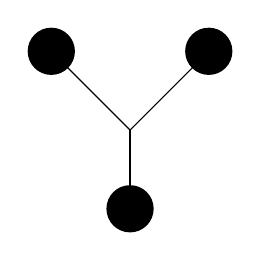
\begin{tikzpicture}
                 \fill[black] (1,1) circle (0.3 cm);
                 \fill[black] (-1,1) circle (0.3 cm);
                 \fill[black] (0,-1) circle (0.3 cm);
                 \draw (0,0) -- (1,1);
                 \draw (0,0) -- (-1,1);
                 \draw (0,0) -- (0,-1);
            \end{tikzpicture}
    \caption{Diagram for term (\ref{termogJ3}) of (\ref{Z_series}).}
    \label{tres}
\end{figure}\\

The number of sources and vertices in a diagram determine the order in $J$ and $g$ of the term in (\ref{Z_series}) that the graph represents.
To reconstruct a term from a diagram, we identify each element in the graph (lines, vertices, blobs), and associate to them the corresponding factor ($m^{-2}$, $g$ and $J$). The complete term is the multiplication of all the factors present in a diagram. As another example, the term linear both in $g$ and $J$ is
\begin{equation}
    \frac{1}{3!}g\qty(\dv{J})^3\times\frac{1}{2!}\qty(\frac{J^2}{2m^2})^2=\qty(\frac{1}{2m^2})^2\frac{4!}{2!}\frac{1}{3!}gJ,
    \label{termogJ}
\end{equation}
resulting from the product of the second term on the first bracket by the third term on the second one in (\ref{expansaozona}). A diagram for this term has one vertex, two propagators, and one source. As vertices must join three lines, one of the propagators must be in a \textit{loop}, as shown by Figure \ref{gJ}.
\begin{figure}[h]
    \centering
    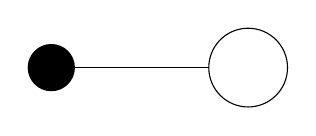
\begin{tikzpicture}
     \fill [black] (0,0) circle (0.3 cm);
    \draw (0,0) -- (2,0);
    \draw (2.5,0) circle (0.5 cm);
    \end{tikzpicture}
    \caption{Diagram for term (\ref{termogJ}) of (\ref{Z_series}) and for term (\ref{gJ_phi3}) of (\ref{Z_1})}
    \label{gJ}
\end{figure}

\section{Feynman diagrams for $\phi^3$ theory}
Integral (\ref{z_toy}) can be regarded as the path integral for a field theory in a single space  dimension (1+1).  Now we consider the usual 3+1 dimensions real scalar field theory. The interaction Lagrangian we will consider is $\mathcal{L}_1=\frac{1}{3!}g\phi^3$, which gives the so-called \textit{phi-cubed} theory. We assume the conditions we required for the validity of the LSZ formula are met, that is
\begin{equation}
 \vev{\phi(x)}=0\quad,\quad \bra{k}{\phi(x)}\ket{0}=e^{-ikx} 
\end{equation}
with one-particle states normalization
\begin{equation}
    \braket{k^\prime}{k}=(2\pi)^32k^0\delta^3(\vb{k}-\vb{k}^\prime).
\end{equation}
To satisfy these, the field can be scaled and shifted, resulting in the Lagrangian
\begin{equation}
    \mathcal{L}=-\frac{1}{2}Z_\phi\partial_\mu\phi\partial^\mu\phi-\frac{1}{2}Z_mm^2\phi^2+\frac{1}{3!}Z_gg\phi^3+Y\phi.
\end{equation}
The functional integral reads
\begin{equation}
    Z(J)=\braket{0}_J=\int\mathcal{D}\phi\,\exp[i\int\dd^4 x\,(\mathcal{L}_0(\phi,\partial_\mu\phi)+\mathcal{L}_1(\phi)+J(x)\phi)]
    \label{path_integral_interacting}
\end{equation}
where we split the Lagrangian as 
\begin{equation}
    \mathcal{L}_0=-\frac{1}{2}\partial_\mu\phi\partial^\mu\phi-\frac{1}{2}m^2\phi^2
    \label{L_0}
\end{equation}
\begin{equation}
    \mathcal{L}_1=\frac{1}{3!}Z_g g \phi^3 + \mathcal{L}_{\text{ct}}
\end{equation}
\begin{equation}
    \mathcal{L}_{\text{ct}}=-\frac{1}{2}(Z_\phi -1)\partial_\mu\phi\partial^\mu\phi-\frac{1}{2}(Z_m-1)m^2\phi^2+Y\phi
    \label{L_ct}
\end{equation}
in order to take advantage of the same procedure we did in (\ref{interac_out}) and our knowledge of the free theory path integral. $\mathcal{L}_{\text{ct}}$ stands for ``counterterm" Lagrangian. As in (\ref{interac_out}), we have
\begin{equation}
    Z(J)=\exp[i\int\dd^4x\,\mathcal{L}_1\qty(\frac{1}{i}\fdv{J(x)})]\int\mathcal{D}\phi\, \exp[i\int\dd^4 x\,(\mathcal{L}_0+J\phi)]
    \label{interac_out_functional}
\end{equation}
where, as we have seen in previous work
\begin{equation}
    Z_0=\int\mathcal{D}\phi\, \exp[i\int\dd^4 x\,(\mathcal{L}_0+J\phi)]=\exp[\frac{i}{2}\int\dd^4x\,\dd^4x^\prime\,J(x)\Delta(x-x^\prime)J(x^\prime)].
\end{equation}

We proceed to calculate (\ref{path_integral_interacting}) ignoring, for now, the counterterms, that is, with interaction Lagrangian being $\mathcal{L}_1=\frac{Z_gg}{3!}\phi^3(x)$ solely. We call this portion of the integral $Z_1$.
\begin{equation}
\begin{aligned}
      Z_1(J)&\propto\exp[\frac{iZ_gg}{3!}\int\dd^4x\,\qty(\frac{1}{i}\fdv{J(x)})^3]Z_0(J)\\
      &=\sum_{V=0}^\infty\frac{1}{V!}\qty[\frac{iZ_gg}{3!}\int\dd^4x\,\qty(\frac{1}{i}\fdv{J(x)})^3]^V\\&\times\sum_{P=0}^{\infty}\frac{1}{P!}\qty[\frac{i}{2}\int\dd^4x\,\dd^4x^\prime\,J(x)\Delta(x-x^\prime)J(x^\prime)]^P,
      \label{Z_1}
\end{aligned}
\end{equation}
which are analogous to (\ref{Z_exps}) and (\ref{Z_series}). Note we have a  proportionality rather than an equality since the $\epsilon$ trick \footnote{Recall we are considering $\mathcal{H}\to(1-i\epsilon)\mathcal{H}$} does not preserve normalization, which will be imposed by hand. Acting with the functional derivatives leaves $E=2P-3V$ sources remaining, and an overall phase of $i^{P-2V}=i^{V+E-P}$ in (\ref{Z_1}). For fixed $V$ and $P$, we have $3V$ functional derivatives acting in $2P$ sources, so there are $(2P)!/(2P-3V)!$ combinations for such arrangements. \\

To enumerate and reconstruct a term from (\ref{Z_1}) we introduce \textit{Feynman diagrams}, in a similar manner we did for our simpler example of last section. We associate:
\begin{itemize}
    \item a propagator $\frac{1}{i}\Delta(x-y)$ to a line connecting points $x$ and $y$;
    \item a source $i\int\dd^4 x\,J(x)$ to a blob at the end or beginning of a line;
    \item an amplitude $iZ_gg\int\dd^4x$ to a vertex joining three lines.
\end{itemize}

To get a sense of what we are doing when constructing these diagrams, we will calculate one term and build its corresponding diagram. We consider a diagram with one vertex and two propagators, that is, the term with $V=1$ and $P=2$ in (\ref{Z_1}), giving $E=2P-3V=1$ \textit{externals}, the remaining number of sources. Our task then is to expand 
\begin{equation}
    \frac{iZ_g g}{2!3!}\int\dd^4x\qty(\frac{1}{i}\fdv{J(x)})^3\qty[\frac{i}{2}\int\dd^4y\,\dd^4zJ(y)\Delta(y-z)J(z)]^2.
    \label{expanding_term}
\end{equation}
A laborious task which goes like this
%Tinha feito umas simplificações e a conta saiu com essas terminologias diferentes, vou arrumar. $\delta_x= \fdv{J(x)}$, $J_y=J(y)$ and $\Delta_{yz}=\Delta(y-z)$
\begin{equation}
    \begin{aligned}
          & = \frac{Z_g g}{2^22!3!}\int\dd^4x\, \qty(\fdv{J(x)})^3\int\dd^4y\,\dd^4z\,\dd^4w\,\dd^4 v J(y)\Delta(y-z)J(z)J(w)\Delta(w-v)J(v)\\
         &\vdots\\ &=\frac{Z_gg}{48}\int\dd^4x\,\dd^4y\,\dd^4z\,\dd^4w\,\dd^4v \Big[\delta^4(y-x)\Delta(y-z)\delta^4(z-x)\delta^4(w-x)\Delta(w-v)J(v)\\
         &\qquad+\delta^4(y-x)\Delta(y-z)\delta^4(z-x)J(w)\Delta(w-v)\delta^4(v-x)+\overbrace{\dots}^{\text{22 terms}}\Big]\\
         &=\frac{Z_gg}{48} \qty[\int\dd^4x\,\dd^4v\Delta(0)\Delta(x-v)J(v)+\int\dd^4x\,\dd^4w\,\Delta(0)J(w)\Delta(w-x)+\overbrace{\dots}^{\text{22 terms}}]
    \end{aligned}
\end{equation}
In the second equality, the other $22$ terms are  just like the ones indicated: all of them consist of three Delta functions, two propagators and one source, but with variables at which these objects are evaluated permuted. In the last line, integration simplify the Deltas in each term, and since the resulting 24 terms differ only by the dummy integration variables, we find
\begin{equation}
    \frac{Z_gg}{2} \int\dd^4x\,\dd^4v\Delta(0)\Delta(x-v)J(v)
    \label{gJ_phi3}.
\end{equation}
This term can be found from the following diagram: $\frac{1}{i}\Delta(0)$ corresponds to a propagator taking a point into itself: a loop. $\frac{1}{i}\Delta(x-y)$ corresponds to a line from $x$ to $y$ and a vertex accounts for $iZ_gg\int\dd^4x$, connecting three lines. We also need a source, which is attached to the free end of the $\Delta(x-y)$. The diagram is assembled as we connect the two ends of $\Delta(0)$ to $\Delta(x-y)$ propagator, being identical to diagram presented in Figure \ref{gJ}.\\

We see that the diagram accounts for everything except for the $1/2$ factor. We now focus on how to determine the numerical factors accompanying a term cast from a diagram. This is the problem of determining how many diagrams correspond to the same term in (\ref{Z_1}). To assess this issue, we note that in the first series of (\ref{Z_1}) (the one summing over $V$), for a given fixed $V$, we can rearrange the order of the three functional derivatives and the order of the $V$ vertices. The swap of derivatives (which effectively swaps the ends of propagators) gives $3!$ different diagrams per vertex, and the swap of vertices gives $V!$ different diagrams. This accounts for $(3!)^VV!$ diagrams to the same term, since these changes leave the diagram invariant. Similarly, in the second series (the one summing over $P$), we can rearrange the two sources and also the $P$ propagators themselves, so there are $(2!)^PP!$ diagrams for the same term. All these factors combined cancel the $((3!)^VV!(2!)^PP!)^{-1}$ factor in (\ref{Z_1}). \\
%some of these multiple rearrangements of sources and propagators give the same diagram then we have overcounted terms and the factors will not exactly cancel,

However, this reasoning can lead to an overcount in some situations. Sometimes the factors don't exactly cancel, just as in our example above (\ref{gJ_phi3}), where we got a $1/2$ left. The overcount in our enumeration considerations is related to some \textit{symmetry} property of a diagram.
%happening whenever rearrangement of propagators gives the same diagram as a rearrangement of sources. 
We must identify how much we have overcounted, so we can divide each term in the series by its corresponding diagram's \textit{symmetry factor}.
%We must be able to identify how many of these terms giving equivalent diagrams there are so we can divide each term in the series by its corresponding diagram's \textit{symmetry factor}, which indicates how much we overcounted that specific term.\\
If we take a look at diagram of Figure (\ref{gJ}) we see that swapping the ends of the loop is equivalent to swapping two legs of the vertex. So there are actually two diagrams corresponding to the same term, thus justifying the $1/2$ factor.\\

Diagram in Figure (\ref{tres}) can also represent a term in (\ref{Z_1}):
 \begin{equation}
     \frac{iZ_g g}{ 3!}\int\dd^4x\,\dd^4y\,\dd^4z\,\dd^4w\, J(y)\Delta(y-x)J(z)\Delta(z-x)J(w)\Delta(w-x).
 \end{equation}
 We have three propagators and any of the $3!$ rearrangements of them gives us the same diagram. This justifies the symmetry factor. Other examples of diagrams are the ones indicated in Figure (\ref{p3v2e0}), with their corresponding symmetry factor. We also highlight an important diagram we will need when dealing with scattering, which that of Figure (\ref{tree_diagramJ}). A complete list of diagrams in $\phi^3$ theory can be found in Chapter 9 of Srednicki \cite{srednicki2007quantum}.\\
 \begin{figure}[h]
    \begin{subfigure}[b]{0.45\textwidth}
    \centering
    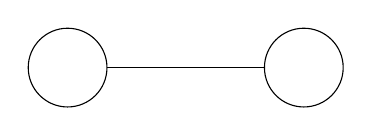
\begin{tikzpicture}
        \draw (1,1) circle (0.5 cm);
        \draw (4,1) circle (0.5 cm);
        \draw (1.5,1) -- (3.5,1); 
    \end{tikzpicture}
    \caption{$S=2^3$}
    \end{subfigure}
    ~ 
    \begin{subfigure}[b]{0.45\textwidth}
    \centering
    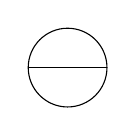
\begin{tikzpicture}
        \draw (1,1) circle (0.5 cm);
        \draw (0.5,1) -- (1.5,1); 
    \end{tikzpicture}
    \caption{$S=2\times 3!$}
    \end{subfigure}
    \caption{Diagrams with $P=3$, $V=2$, $E=0$.}
\label{p3v2e0}
\end{figure}
\begin{figure}
    \centering
                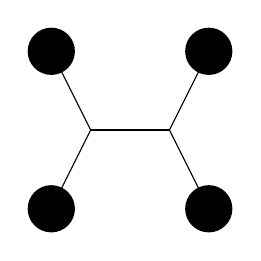
\begin{tikzpicture}
                \fill[black] (1,1) circle (0.3 cm);
                 \fill[black] (-1,1) circle (0.3 cm);
                 \fill[black] (-1,-1) circle (0.3cm);
                 \fill[black] (1,-1) circle (0.3 cm);
                 \draw (-0.5,0) -- (0.5,0);
                 \draw (-1,1) -- (-0.5,0);
                 \draw (1,1) -- (0.5,0);
                 \draw (-1,-1) -- (-0.5,0);
                 \draw (1,-1) -- (0.5,0);
            \end{tikzpicture}
    \caption{Diagram with $P=5$, $V=2$, $E=4$, and $S=2^3$.}
    \label{tree_diagramJ}
\end{figure}


\section{The path integral as the sum of connected diagrams}
Diagrams we dealt so far are all connected:  every two points can be connected by the trace of, say, a pen, continuously. However $Z(J)$ must include also other contributions arising from more general diagrams. The most general diagram $D$ is composed of the product of connected diagrams $C_I$
\begin{equation}
    D=\prod_{I}C_I^{n_I}
\end{equation}
where $C_I$ is the $I$-th connected diagram (with its symmetry factor included) and $n_I$ is the number of $C_I$'s present in $D$. However, since exchanges of propagators and vertices among different connected diagrams can result in the same diagrams, we must include an additional symmetry factor $S_D$. The exchanges that can leave the diagram unchanged are those performed between different but identical connected diagrams $C_I$. Since there are $n_I$ $C_I$'s in $D$, we can conclude that $S_D=\prod_I n_I!$, so that a general diagram reads
\begin{equation}
    D=\prod_{I}\frac{1}{n_I!}C_I^{n_I}
\end{equation}
Equation (\ref{Z_1}) tell us that $Z(J)$ is proportional to the sum over diagrams and, since diagrams are labeled by $n_I$, then
\begin{equation}
\begin{aligned}
        Z_1(J)\propto&\sum_{\{n_I\}}D\\=&\sum_{\{n_I\}}\prod_{I}\frac{1}{n_I!}C_I^{n_I}\\
        =&\sum_{n_1,n_2\dots}\frac{1}{n_1!}C_1^{n_1}\frac{1}{n_2!}C_2^{n_2}\dots\\
        =&\prod_I\sum_{n_I=0}^\infty\frac{1}{n_I!}C_I^{n_I}\\
        =&\prod_I\exp(C_I)\\
        =&\exp\sum_IC_I.
\end{aligned}
\end{equation}
A remarkable result, indicating that $Z_1(J)$ is proportional to the exponential of the sum of connected diagrams. This readily gives us a normalization criterion: if we wish $Z_1(0)=1$ we must omit \textit{vacuum diagrams} from the sum: those with no sources. With this convention we pretend vacuum diagrams don't even exist, we simply don't count them. Then, the sum of connected diagrams with no sources equals zero. We write
\begin{equation}
    Z_1(J)=\exp [iW_1(J)]
\end{equation}
where
\begin{equation}
    iW_1(J)=\sum_{I\neq\{0\}}C_I
\end{equation}
is the sum of connected diagrams omitting vacuum diagrams.\\
\section{Dealing with counterterms}
\subsection{Tadpoles}
So far we have been ignoring the other terms in the interaction Lagrangian. We analyze the consequences this leads to. The vacuum expectation value of the field is
\begin{equation}
\begin{aligned}
        \vev{\phi(x)}=&\frac{1}{i}\fdv{J(x)}Z_1(J)\eval_{J=0}\\
        =&\fdv{J(x)}W_1(J)\eval_{J=0}
\end{aligned}
\label{1Pcorrelation}
\end{equation}
In the last equality, the functional derivative removes a source from the sum of diagrams, and then, when we evaluate the derivative at $J=0$, we are left only with the diagrams that had a single source, but now have this source removed. One of these diagrams is the one shown in Figure (\ref{gJ}) with its source removed, adding the others:
\begin{equation}
    \begin{aligned}
        \vev{\phi(x)}&=
        \begin{gathered}
        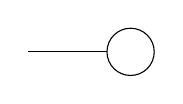
\begin{tikzpicture}
        \draw (0,0) -- (1,0);
        \draw (1.3,0) circle [radius=0.3cm];
        \end{tikzpicture}
        \end{gathered}+
        \begin{gathered}
        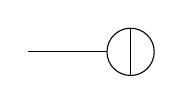
\begin{tikzpicture}
        \draw (0,0) -- (1,0);
        \draw (1.3,0) circle [radius=0.3cm];
        \draw (1.3,0.3) -- (1.3,-0.3);
        \end{tikzpicture}
        \end{gathered}+
        \begin{gathered}
        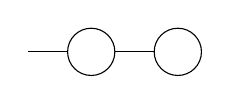
\begin{tikzpicture}
        \draw (0,0) -- (0.5,0);
        \draw (0.8,0) circle [radius=0.3cm];
        \draw (1.1,0) -- (1.6,0);
        \draw (1.9,0) circle [radius=0.3cm];
        \end{tikzpicture}
        \end{gathered}+       
        \begin{gathered}
        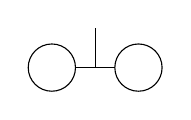
\begin{tikzpicture}
        \draw (1.35,0) -- (1.35,0.5);
        \draw (0.8,0) circle [radius=0.3cm];
        \draw (1.1,0) -- (1.6,0);
        \draw (1.9,0) circle [radius=0.3cm];
        \end{tikzpicture}
        \end{gathered}
    \\&=\frac{1}{2}iZ_gg\int\dd^4y\frac{1}{i}\Delta(x-y)\frac{1}{i}\Delta(0)+\order{g^3}.
    \end{aligned}
\end{equation}
In the last line we translated only the diagram linear in $g$. The point here is that $\vev{\phi(x)}$ is not zero, as  required by LSZ formula. This is no big news, since we are ignoring the other terms in the Lagrangian. To fix the expectation value, it's sufficient to consider the linear term $Y\phi$ from $\mathcal{L}_{\text{ct}}$, so that the interaction Lagrangian now reads
\begin{equation}
    \mathcal{L}_1=\frac{1}{3!}Z_gg\phi^3+Y\phi
\end{equation}
and (\ref{Z_1}) gets a new term
\begin{equation}
\begin{aligned}
        Z_Y(J)=&\exp\qty[\frac{1}{3!}iZ_gg\int\dd^4x\qty(\frac{1}{i}\fdv{J(x})^3+iY\int\dd^4x\, \frac{1}{i}\fdv{J(x)}]Z_0(J)\\
        =&\exp\qty[iY\int\dd^4x\, \frac{1}{i}\fdv{J(x)}]Z_1(J)\\
        =&\sum_{X=0}^\infty\frac{1}{X!}\qty[iY\int\dd^4x\, \frac{1}{i}\fdv{J(x)}]^XZ_1(J).
\end{aligned}
\label{ZY}
\end{equation}
This gives us a new series and introduce a new vertex to our diagrams: those corresponding to $iY\int\dd^4y$. The diagrams for the $X=0$ terms are all the previous diagrams we have been dealing so far. Since, for $P=2$ and $V=1$, we know the diagram for $Z_1$ linear in $g$ is that of Figure (\ref{gJ}) we built before. Now, if we consider $X=1$ in (\ref{ZY}) we get the term linear in $g$ and in $Y$:
\begin{equation}
\begin{aligned}
   Z_Y(J)&=iY \frac{Z_gg}{2}\int\dd^4x^\prime\frac{1}{i}\fdv{J(x^\prime)}
   \int\dd^4x\,\dd^4y\Delta(0)\Delta(x-y)J(y)+\order{g^3}\\
   &= \frac{YZ_gg}{2}\int\dd^4x^\prime
   \dd^4x\,\Delta(0)\Delta(x-x^\prime)+\order{g^3}
\end{aligned}
\end{equation}
which can be represented by the following diagram
\begin{equation}
    Z_Y(J)=
    \begin{gathered}
        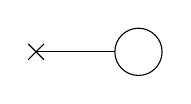
\begin{tikzpicture}
        \draw (0,0) -- (1,0);
        \draw (-0.1,-0.1) -- (0.1,0.1);
        \draw (-0.1,0.1) -- (0.1,-0.1);
        \draw (1.3,0) circle [radius=0.3cm];
        \end{tikzpicture}
        \end{gathered}
        \label{tadpole}
\end{equation}
where the line abruptly ending in a ``x" corresponds to our new vertex $iY\int\dd^4 y$. Other examples of connected diagrams with vertices from the linear counterterm are shown in Figure (\ref{diagramaX}).\\

\begin{figure}[h]
    \begin{subfigure}[]{0.2\textwidth}
    \centering
    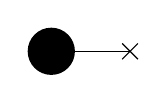
\begin{tikzpicture}
     \fill [black] (0,0) circle (0.3 cm);
    \draw (0,0) -- (1,0);
    \draw (0.9,-0.1) -- (1.1, 0.1);
    \draw (0.9,0.1) -- (1.1, -0.1);
    \end{tikzpicture}
%    \caption{$S=1$}
    \end{subfigure}
    ~ 
    \begin{subfigure}[]{0.3\textwidth}
    \centering
    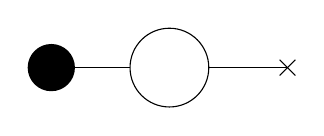
\begin{tikzpicture}
     \fill [black] (0,0) circle (0.3 cm);
    \draw (0,0) -- (1,0);
    \draw (1.5,0) circle (0.5 cm);
    \draw (2,0) -- (3,0);
    \draw (2.9,-0.1) -- (3.1, 0.1);
    \draw (2.9,0.1) -- (3.1, -0.1);
    \end{tikzpicture}
%    \caption{$S=2$}
        \end{subfigure}
    ~
    \begin{subfigure}[]{0.2\textwidth}
    \centering
    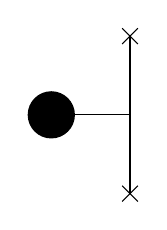
\begin{tikzpicture}
     \fill [black] (0,0) circle (0.3 cm);
    \draw (0,0) -- (1,0);
    \draw (1,-1) -- (1,1);
    \draw (0.9,-1.1) -- (1.1, -0.9);
    \draw (0.9,-0.9) -- (1.1, -1.1);
    \draw (0.9,1.1) -- (1.1, 0.9);
    \draw (0.9,0.9) -- (1.1, 1.1);
    \end{tikzpicture}
%    \caption{$S=2$}
    \end{subfigure}
    ~
    \begin{subfigure}[]{0.2\textwidth}
    \centering
    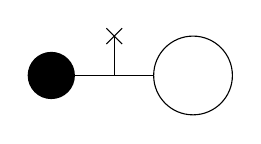
\begin{tikzpicture}
     \fill [black] (0,0) circle (0.3 cm);
    \draw (0,0) -- (1.3,0);
    \draw (1.8,0) circle (0.5 cm);
    \draw (0.8,0) -- (0.8,0.5);
    \draw (0.7,0.4) -- (0.9,0.6);
    \draw (0.7,0.6) -- (0.9,0.4);
    \end{tikzpicture}
%    \caption{$S=2$}
    \end{subfigure}
    \caption{Diagrams for (\ref{ZY}) with $E=1$, $X\geq1$}
\label{diagramaX}
\end{figure}

The same reasoning we did previously tells us that $Z_Y(J)$ equals the exponential of the sum of connected diagrams and, again, we omit vacuum diagrams (such as (\ref{tadpole})) to ensure normalization. When computing the VEV of (\ref{1Pcorrelation}), we again find it equal the sum of single source diagrams, with the sources removed. The difference now is that we include the diagrams with $X\neq 0$, such as the ones in Figure (\ref{diagramaX}). We assert that $Y=\order{g}$ and $Z_g=1+\order{g^2}$ \cite{srednicki2007quantum}, so, up to $\order{g}$, we consider $Z_g=1$ and the correlation reads
\begin{equation}
\begin{aligned}
   \vev{\phi(x)}&=
   \begin{gathered}
    \begin{tikzpicture}
    \draw (0,0) -- (1,0);
    \draw (0.9,-0.1) -- (1.1, 0.1);
    \draw (0.9,0.1) -- (1.1, -0.1);
    \end{tikzpicture}
   \end{gathered}+
   \begin{gathered}
        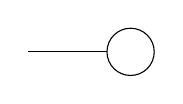
\begin{tikzpicture}
        \draw (0,0) -- (1,0);
        \draw (1.3,0) circle [radius=0.3cm];
        \end{tikzpicture}
    \end{gathered}+\order{g^3}\\
   &=\qty(iY+\frac{1}{2}i g\frac{1}{i}\Delta(0))\int\dd^4y\frac{1}{i}\Delta(x-y)+\order{g^3}.
\end{aligned}
\end{equation}
Therefore, to attain the LSZ condition, we need
\begin{equation}
    Y=\frac{1}{2}ig\Delta(0)+\order{g^3}
    \label{1pcoorelation_X}
\end{equation}
so that $\vev{\phi(x)}=0$. Being present in the Lagrangian, we know that $Y$ must be real so 
\begin{equation}
    \Delta(0)=\int\frac{\dd^4k}{(2\pi)^4}\frac{1}{k^2+m^2-i\epsilon}
\end{equation}
must be purely imaginary. The problem  is that this integral diverges, so we need to find a way to implement an ultraviolet cutoff. This cutoff is subtly implemented by considering 
\begin{equation}
    \Delta(x-y)=\int\frac{\dd^4k}{(2\pi)^4}\frac{e^{ik(x-y)}}{k^2+m^2-i\epsilon}\qty[\frac{\Lambda^2}{k^2+\Lambda^2-i\epsilon}]^2
\end{equation}
This way $\Delta(0)=i\Lambda^2/(16\pi^2)$, and we are in the position to take $\Lambda\to\infty$, making $Y\to\infty$ while $\vev{\phi(x)}=0$ \cite{srednicki2007quantum}. If we wish to calculate (\ref{1pcoorelation_X}) to higher order in $g$ we must consider the other diagrams of equation (\ref{1Pcorrelation}) and of Figure (\ref{diagramaX}).

Result (\ref{1pcoorelation_X}) indicates that the sum of diagrams of a single source, with that source removed, equals zero when considering the linear counterterm. The remarkable statement now is that if we replace that single source that gets removed by any other sub-diagram, the result still holds, the sum still vanishes. This is because if we replace the single source by the sub-diagram whose translation in terms of sources, propagators and vertices reads $\text{sub(x)}$, then the complete diagram, with a source replaced by $\text{sub(x)}$ reads $\int \dd^4x\,\text{sub(x)}\,\text{main}(x)$, where $\text{main}(x)$ is the sum of diagrams with a single source with that source removed, i.e. $\vev{\phi(x)}=0$. Thus $\int\dd^4x\,\text{sub(x)}\vev{\phi(x)}=0$. The diagrams responsible for this fact are those introduced by the linear counterterm. Diagrams cancelled with the linear counterterms are called \textit{tadpoles}. They are the ones that, when a single line is cut, leaves the diagram divided into two parts, one of which has no sources. Since they cancel with linear counterterms, we take as convention to simply ignore linear counterterms and the tadpoles altogether. \\
\subsection{Other counterterms}
We now focus on the remaining counterterms $-\frac{1}{2}(Z_\phi -1)\partial_\mu\phi\partial^\mu\phi-\frac{1}{2}(Z_m-1)m^2\phi^2$. We rename $A=Z_\phi-1$ and $B=Z_m-1$ (both of the order of $\order{g^2}$) so that the path integral reads
\begin{equation}
    Z(J)=\exp{-\frac{i}{2}\int\dd^4x\,\qty[A\partial^\mu\qty(\frac{1}{i}\fdv{j(x)})\partial_\mu\qty(\frac{1}{i}\fdv{J(x)})+\frac{1}{2}Bm^2\qty(\frac{1}{i}\fdv{J(x)})^2]}Z_Y.
\end{equation}
Integration by parts allows us to write
\begin{equation}
    Z(J)=\exp[-\frac{i}{2}\int\dd^4x\qty(\frac{1}{i}\fdv{J(x)})\qty(-A\partial^2+Bm^2)\qty(\frac{1}{i}\fdv{J(x)})]Z_Y
\end{equation}
This gives rise to a new vertex where two lines meet, for which we associate $-i\int\dd^4x(-A\partial^2+Bm^2)$. Since the lowest of these diagrams are already of the order of $g^2$, we won't be dealing with them. The diagrams we will be considering for the sum of connected diagrams $iW(J)$, thus, are the ones with or more sources, and we will ignore tadpoles and the ones arising from the linear counterterm. They are shown below, up to $g^4$. 
\begin{equation}
    \begin{aligned}
    iW(J)&=
       \begin{gathered}
            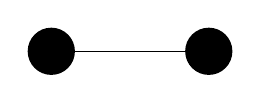
\begin{tikzpicture}
                \draw (0,0) -- (2,0);
                \fill [black] (0,0) circle (0.3 cm);
                \fill [black] (2,0) circle (0.3 cm);
            \end{tikzpicture}
       \end{gathered}
       +\begin{gathered}
            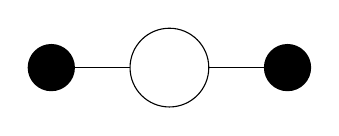
\begin{tikzpicture}
                \fill [black] (0,0) circle (0.3 cm);
                \draw (0,0) -- (1,0);
                \draw (1.5,0) circle (0.5 cm);
                \draw (2,0) -- (3,0);
                \fill [black] (3,0) circle (0.3 cm);
            \end{tikzpicture}
       \end{gathered}+
       \begin{gathered}
            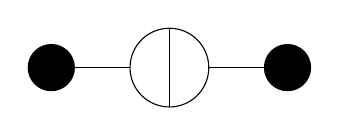
\begin{tikzpicture}
                \fill [black] (0,0) circle (0.3 cm);
                \draw (0,0) -- (1,0);
                \draw (1.5,0) circle (0.5 cm);
                \draw (2,0) -- (3,0);
                \fill [black] (3,0) circle (0.3 cm);
                \draw (1.5,0.5)--(1.5,-0.5);
            \end{tikzpicture}
       \end{gathered}\\
       &+\begin{gathered}
            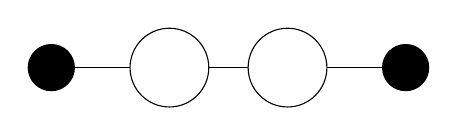
\begin{tikzpicture}
                \fill [black] (0,0) circle (0.3 cm);
                \draw (0,0) -- (1,0);
                \draw (1.5,0) circle (0.5 cm);
                \draw (2,0) -- (2.5,0);
                \draw (3,0) circle (0.5 cm);
                \draw (3.5,0) -- (4.5,0);
                \fill [black] (4.5,0) circle (0.3 cm);
            \end{tikzpicture}
       \end{gathered}+
       \begin{gathered}
            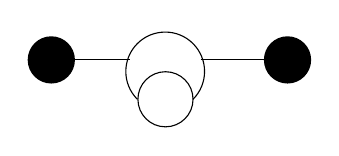
\begin{tikzpicture}
                \fill [black] (0,0) circle (0.3 cm);
                \draw (0,0) -- (1,0);
                \draw (1.8,-0.5) arc (-45:225:0.5);
                \draw (1.895,0) -- (3,0);
                \fill [black] (3,0) circle (0.3 cm);
                \draw (1.45,-0.5) circle (0.35);
            \end{tikzpicture}
       \end{gathered}\\
       &+
       \begin{gathered}
            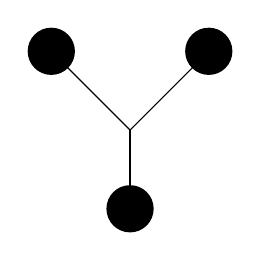
\begin{tikzpicture}
                 \fill[black] (1,1) circle (0.3 cm);
                 \fill[black] (-1,1) circle (0.3 cm);
                 \fill[black] (0,-1) circle (0.3 cm);
                 \draw (0,0) -- (1,1);
                 \draw (0,0) -- (-1,1);
                 \draw (0,0) -- (0,-1);
            \end{tikzpicture}
       \end{gathered}+
       \begin{gathered}
            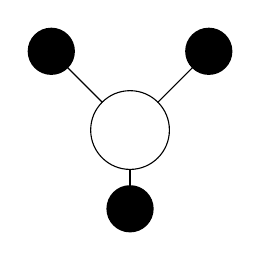
\begin{tikzpicture}
                 \fill[black] (1,1) circle (0.3 cm);
                 \fill[black] (-1,1) circle (0.3 cm);
                 \fill[black] (0,-1) circle (0.3 cm);
                 \draw (0.35,0.35) -- (1,1);
                 \draw (-0.35,0.35) -- (-1,1);
                 \draw (0,-0.5) -- (0,-1);
                 \draw (0,0) circle (0.5 cm);
            \end{tikzpicture}
       \end{gathered}+
       \begin{gathered}
            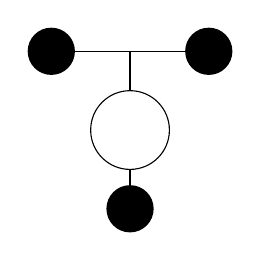
\begin{tikzpicture}
                \fill[black] (1,1) circle (0.3 cm);
                 \fill[black] (-1,1) circle (0.3 cm);
                 \fill[black] (0,-1) circle (0.3 cm);
                 \draw (-1,1) -- (1,1);
                 \draw (0,1) -- (0,0.5);
                 \draw (0,-0.5) -- (0,-1);
                 \draw (0,0) circle (0.5 cm);
            \end{tikzpicture}
       \end{gathered}+
       \begin{gathered}
            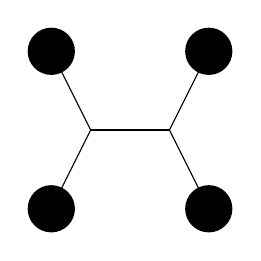
\begin{tikzpicture}
                \fill[black] (1,1) circle (0.3 cm);
                 \fill[black] (-1,1) circle (0.3 cm);
                 \fill[black] (-1,-1) circle (0.3cm);
                 \fill[black] (1,-1) circle (0.3 cm);
                 \draw (-0.5,0) -- (0.5,0);
                 \draw (-1,1) -- (-0.5,0);
                 \draw (1,1) -- (0.5,0);
                 \draw (-1,-1) -- (-0.5,0);
                 \draw (1,-1) -- (0.5,0);
            \end{tikzpicture}
       \end{gathered}\\
       &+\begin{gathered}
            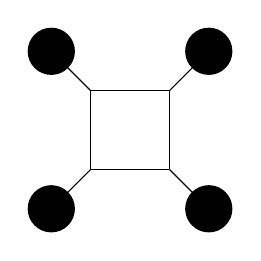
\begin{tikzpicture}
                \fill[black] (1,1) circle (0.3 cm);
                 \fill[black] (-1,1) circle (0.3 cm);
                 \fill[black] (-1,-1) circle (0.3cm);
                 \fill[black] (1,-1) circle (0.3 cm);
                 \draw (-0.5,0.5) -- (-0.5,0.5);
                 \draw (-0.5,-0.5) -- (-0.5,0.5);
                 \draw (-0.5,-0.5) -- (0.5,-0.5);
                 \draw (-0.5,0.5) -- (0.5,0.5);
                 \draw (0.5,0.5) -- (0.5,-0.5);
                 \draw (-1,1) -- (-0.5,0.5);
                 \draw (1,1) -- (0.5,0.5);
                 \draw (-1,-1) -- (-0.5,-0.5);
                 \draw (1,-1) -- (0.5,-0.5);
            \end{tikzpicture}
       \end{gathered}+
        \begin{gathered}
            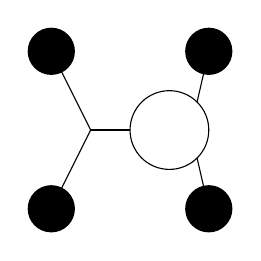
\begin{tikzpicture}
                \fill[black] (1,1) circle (0.3 cm);
                 \fill[black] (-1,1) circle (0.3 cm);
                 \fill[black] (-1,-1) circle (0.3cm);
                 \fill[black] (1,-1) circle (0.3 cm);
                 \draw (0.5,0) circle (0.5 cm);
                 \draw (-0.5,0) -- (0,0);
                 \draw (-1,1) -- (-0.5,0);
                 \draw (1,1) -- (0.85,0.35);
                 \draw (-1,-1) -- (-0.5,0);
                 \draw (1,-1) -- (0.85,-0.35);
            \end{tikzpicture}
       \end{gathered}+
        \begin{gathered}
            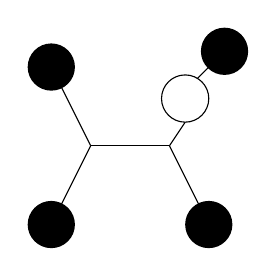
\begin{tikzpicture}
                \fill[black] (1.2,1.2) circle (0.3 cm);
                 \fill[black] (-1,1) circle (0.3 cm);
                 \fill[black] (-1,-1) circle (0.3cm);
                 \fill[black] (1,-1) circle (0.3 cm);
                 \draw (-0.5,0) -- (0.5,0);
                 \draw (-1,1) -- (-0.5,0);
                 \draw (0.7,0.3) -- (0.5,0);
                 \draw (-1,-1) -- (-0.5,0);
                 \draw (1,-1) -- (0.5,0);
                 \draw (0.85,0.85) -- (1.2,1.2);
                 \draw (0.7,0.6) circle (0.3cm);
            \end{tikzpicture}
       \end{gathered}+
       \begin{gathered}
            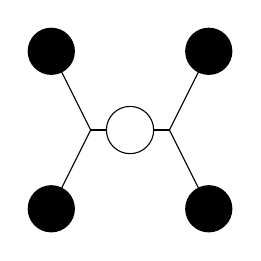
\begin{tikzpicture}
                \fill[black] (1,1) circle (0.3 cm);
                 \fill[black] (-1,1) circle (0.3 cm);
                 \fill[black] (-1,-1) circle (0.3cm);
                 \fill[black] (1,-1) circle (0.3 cm);
                 \draw (-0.5,0) -- (-0.3,0);
                 \draw (0.3,0) -- (0.5,0);
                 \draw (-1,1) -- (-0.5,0);
                 \draw (1,1) -- (0.5,0);
                 \draw (-1,-1) -- (-0.5,0);
                 \draw (1,-1) -- (0.5,0);
                 \draw (0,0) circle (0.3 cm);
            \end{tikzpicture}
       \end{gathered}+\order{g^5}
    \end{aligned}
    \label{iWphi3}
\end{equation}
\section{Feynman diagrams for $\phi^4$ theory}
For this theory, we consider the Lagrangian $\mathcal{L}=\mathcal{L}_0+\mathcal{L}_1$ where now
\begin{equation}
    \mathcal{L}_1=-\frac{1}{4!}Z_\lambda\lambda\phi^4(x)+\mathcal{L}_{\text{ct}},
\end{equation}
$\mathcal{L}_0$ and $\mathcal{L}_{\text{ct}}$ are as in (\ref{L_0}) and (\ref{L_ct}), respectively. Again, the functional integral takes the form of (\ref{interac_out_functional}). Ignoring counterterms, we have
\begin{equation}
    Z(J)=\sum_{V=0}^\infty\frac{1}{V!}\qty[\frac{iZ_\lambda\lambda}{4!}\int\dd^4x\qty(\frac{1}{i}\fdv{J(x)})^4]^V\sum_{P=0}^\infty\frac{1}{P!}\qty[\frac{i}{2}\int\dd^4x\,\dd^4y\,J(x)\Delta(x-y)J(y)]^P.
\end{equation}
The functional derivatives act on the propagators leaving $E=2P-4V$ sources remaining and an overall phase $i^{P-3V}=i^{E+V-P}$. Feynman diagrams are built according to these rules:
\begin{itemize}
    \item A vertex is where \textit{four lines} meet, and we associate $iZ_\lambda\lambda\int\dd^4x$ to it.
    \item A source is represented by a blob, and we associate $i\int\dd^4x\,J(x)$ for each one of them
    \item A line joining points $x$ and $y$ corresponds to the propagator $\frac{1}{i}\Delta(x-y)$
\end{itemize} 
The contributions to the sum of connected diagrams with $0<V\leq2$ and $0<E\leq4$ (omitting vacuum diagrams) are shown below.\\
\begin{equation}
    \begin{aligned}
    iW_1(J)&=
    \begin{gathered}
        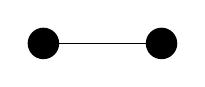
\begin{tikzpicture}
        \fill [black] (0,0) circle (0.2 cm);
        \draw (0,0) -- (1.5,0);
        \fill[black] (1.5,0) circle (0.2cm);
        \end{tikzpicture}
    \end{gathered}+
    \begin{gathered}
        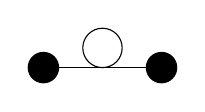
\begin{tikzpicture}
        \fill [black] (0,0) circle (0.2 cm);
        \draw (0,0) -- (1.5,0);
        \fill[black] (1.5,0) circle (0.2cm);
        \draw (0.75,0.25) circle (0.25 cm);
        \end{tikzpicture}
    \end{gathered}+
    \begin{gathered}
        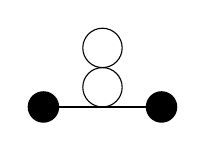
\begin{tikzpicture}
        \fill [black] (0,0) circle (0.2 cm);
        \draw (0,0) -- (1.5,0);
        \fill[black] (1.5,0) circle (0.2cm);
        \draw (0.75,0.25) circle (0.25 cm);
        \draw (0.75,0.75) circle (0.25 cm);
        \end{tikzpicture}
    \end{gathered}+
    \begin{gathered}
        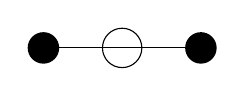
\begin{tikzpicture}
        \fill [black] (0,0) circle (0.2 cm);
        \draw (0,0) -- (2,0);
        \fill[black] (2,0) circle (0.2cm);
        \draw (1,0) circle (0.25 cm);
        \end{tikzpicture}
    \end{gathered}\\
    &+\begin{gathered}
        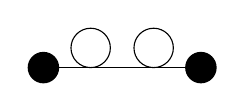
\begin{tikzpicture}
        \fill [black] (0,0) circle (0.2 cm);
        \draw (0,0) -- (2,0);
        \fill[black] (2,0) circle (0.2cm);
        \draw (0.6,0.25) circle (0.25 cm);
        \draw (1.4,0.25) circle (0.25 cm);
        \end{tikzpicture}
    \end{gathered}+
    \begin{gathered}
        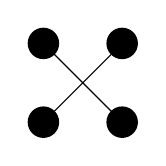
\begin{tikzpicture}
        \fill [black] (-0.5,-0.5) circle (0.2 cm);
        \fill [black] (-0.5,0.5) circle (0.2 cm);
        \fill [black] (0.5,0.5) circle (0.2 cm);
        \fill [black] (0.5,-0.5) circle (0.2 cm);
        \draw (-0.5,-0.5) -- (0.5,0.5);
        \draw (-0.5,0.5) -- (0.5,-0.5);
        \end{tikzpicture}
    \end{gathered}+
    \begin{gathered}
        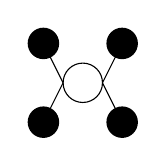
\begin{tikzpicture}
        \fill [black] (-0.5,-0.5) circle (0.2 cm);
        \fill [black] (-0.5,0.5) circle (0.2 cm);
        \fill [black] (0.5,0.5) circle (0.2 cm);
        \fill [black] (0.5,-0.5) circle (0.2 cm);
        \draw (0,0) circle (0.25 cm);
        \draw (-0.5,-0.5) -- (-0.25,0);
        \draw (-0.5,0.5) -- (-0.25,0);
        \draw (0.5,0.5) -- (0.25,0);
        \draw (0.5,-0.5) -- (0.25,0);
        \end{tikzpicture}
    \end{gathered}+
    \begin{gathered}
        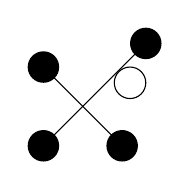
\begin{tikzpicture}
        \fill [black] (-0.5,-0.5) circle (0.2 cm);
        \fill [black] (-0.5,0.5) circle (0.2 cm);
        \fill [black] (0.8,0.8) circle (0.2 cm);
        \fill [black] (0.5,-0.5) circle (0.2 cm);
        \draw (-0.5,-0.5) -- (0.8,0.8);
        \draw (-0.5,0.5) -- (0.5,-0.5);
        \draw (0.6,0.3) circle (0.2 cm);
        \end{tikzpicture}
    \end{gathered}
    +\order{\lambda^3}
    \end{aligned}
    \label{W_phi4}
\end{equation}

We analyze the vacuum expectation value for the field in $\phi^4$ to check the consistency with the requirement from the LSZ formula:
\begin{equation}
    \vev{\phi(x)}=\frac{1}{i}\fdv{J(x)}Z_1(J)\eval_{J=0}
    \label{vevphi4}
\end{equation}
since $Z_1(J)=\exp[iW_1]$, (\ref{vevphi4}) is
\begin{equation}
    \vev{\phi(x)}=\fdv{J(x)}W_1\eval_{J=0}
\end{equation}
the sum of diagrams with a single source, with that source removed. As (\ref{W_phi4}) tells us, there are no diagrams of a single source contributing, so $\vev{\phi(x)}$ is precisely zero, and we are in good terms with the requirements from LSZ formula without having to introduce a linear counterterm. Ignoring also the other counterterms, we can take $iW(J)=iW_1(J)$ and $Z(J)=Z_1(J)$.



\chapter{Path Integrals for Interacting Complex Scalar Fields}
\section{The complex scalar field}
\subsection{Lagrangian, equations of motion, conjugate momenta and Hamiltonian}
So far we have worked solely with the real scalar field. Now we consider the Lagrangian density
\begin{equation}
\mathcal{L}=-\partial^{\mu} \phi^{\dagger} \partial_{\mu} \phi-{m}^{2} \phi^{\dagger} \phi+\Omega_{0}
\end{equation}
with the action being $S=\int\dd^4 x\, \mathcal{L}$. We treat $\phi$ and $\phi^\dagger$ as independent field variables and the equations of motion follow from the variational principle
\begin{equation}
    -\fdv{S}{\phi^\dagger}=-\pdv{\mathcal{L}}{\phi^\dagger}+\partial_\mu\pdv{\mathcal{L}}{(\partial_\mu\phi^\dagger)}=(-\partial^2+m^2)\phi=0
    \label{eom1}
\end{equation}
\begin{equation}
    -\fdv{S}{\phi}=-\pdv{\mathcal{L}}{\phi}+\partial_\mu\pdv{\mathcal{L}}{(\partial_\mu\phi)}=(-\partial^2+m^2)\phi^\dagger=0
    \label{eom2}
\end{equation}
so that both $\phi$ and $\phi^\dagger$ obey the Klein-Gordon equation. The conjugate momenta are
\begin{equation}
    \Pi(x)=\pdv{\mathcal{L}}{\dot{\phi}}=\dot{\phi}^\dagger
\end{equation}
\begin{equation}
    \Pi^\dagger(x)=\pdv{\mathcal{L}}{\dot{\phi}^\dagger}=\dot{\phi}
\end{equation}
so the Hamiltonian density $\mathcal{H}=\Pi(x) \dot{\phi}+\Pi^{\dagger}(x) \dot{\phi}^{\dagger}-\mathcal{L}$ reads
\begin{equation}
\mathcal{H}=\Pi^{\dagger}(x) \Pi(x)+\nabla \phi^{\dagger} \nabla \phi+m^{2} \phi^{\dagger} \phi-\Omega_{0}.
\end{equation}
From equations (\ref{eom1}) and (\ref{eom2}), the following mode expansion arises as a solution
\begin{equation}
     \phi(x)=\int\widetilde{\dd k}\, [a(\vb{k})e^{ikx}+b^\dagger(\vb{k})e^{-ikx}].
\end{equation}
multiplying this mode expansion by exponentials and integrating over space allows us to find
\begin{equation}
a(\mathbf{k})=\int \dd^{3} x\, e^{-i k x}\left(\omega \phi(x)+i \partial_{0} \phi(x)\right)
\label{azinho}
\end{equation}
\begin{equation}
b(\mathbf{k})=\int \dd^{3}x\, e^{-i k x}\left(\omega \phi^\dagger(x)+i \partial_{0} \phi^\dagger(x)\right)
\label{bzinho}
\end{equation}
With $a^\dagger$ and $b^\dagger$ following from hermitian conjugation. The relevant commutation relations at equal times are
\begin{equation}
\begin{aligned}
\comm{\phi(x)}{\Pi(x^\prime)}&=i\delta^3(\vb{x}-\vb{x}^\prime)\\
\comm{\phi^\dagger(x)}{\Pi^\dagger(x^\prime)}&=i\delta^3(\vb{x}-\vb{x}^\prime)
\end{aligned}
\end{equation}
with other possible combinations between $\phi$, $\Pi$, $\phi^\dagger$ and $\Pi^\dagger$ vanishing. From (\ref{azinho}) and (\ref{bzinho}) and their conjugates, we can check that
\begin{equation}
    \begin{aligned}
    \comm{a(\vb{k})}{a^\dagger(\vb{k}^\prime)}&=(2\pi)^3 2\omega \delta^3(\vb{k}-\vb{k}^\prime)\\
    \comm{b(\vb{k})}{b^\dagger(\vb{k}^\prime)}&=(2\pi)^3 2\omega \delta^3(\vb{k}-\vb{k}^\prime)
    \end{aligned}
\end{equation}
with other combinations  vanishing. $a^\dagger(\vb{k})$ and $b^\dagger(\vb{k})$ and their conjugates are creation and annihilation operators. This highlights that, in the case of the complex field, there are two types of particles: those created by $b^\dagger$ and those created by $a^\dagger$ when they act on the vacuum state $\ket{0}$, assumed to be normalized $\braket{0}=1$ and to vanish upon the action of annihilation operators $a(\vb{k})\ket{0}=b(\vb{k})\ket{0}=0$ for any $\vb{k}$.\\

Expressing the total Hamiltonian in terms of the creation and annihilation operators gives
\begin{equation}
H=-\Omega_{0} V+\int \widetilde{d k}\,\omega\left[a^{\dagger}(\vb{k}) a(\vb{k})+b^{\dagger}(\vb{k}) b(\vb{k})+(2 \pi)^{3} 2 \omega \delta^{3}(\vb{0})\right].
\end{equation}
Interpreting $(2\pi)^3\delta^3(\vb{0})$ as the volume of space and integrating the last term up to a cutoff gives
\begin{equation}
    H=(2\mathcal{E}_0-\Omega_0)V+\int \widetilde{d k}\,\omega\left[a^{\dagger}(\vb{k}) a(\vb{k})+b^{\dagger}(\vb{k}) b(\vb{k})\right]
\end{equation}
where $\mathcal{E}_0=\frac{1}{2(2\pi)^3}\int\dd^3 k\,\omega$ integrated up to a cutoff $\Lambda$ is the zero point energy density of the oscillators. We set $\Omega_0=2\mathcal{E}_0$ to make the Hamiltonian ground state equal to zero.
\subsection{The LSZ formula for the complex scalar field}
Since there are two types of particles in a complex theory, we can have different combinations of types of particles  when preparing initial and final states for the $\braket{f}{i}$ amplitude.
%When there is only one kind of particle involved in both the initial and final states, we use the the LSZ formula we already derived. 
Following similar steps we took when deriving the LSZ for the first time, it is easy to show that the LSZ formula, for initial and final states with $a$- and $b$-type particles, for instance, reads
\begin{equation}
\begin{aligned}
        \braket{f}{i}&=\vev{\text{T}a_{1^\prime}(+\infty)b_{2^\prime}(+\infty)a^\dagger_1(-\infty)b^\dagger_2(-\infty)}\\
        &=i^4\int \dd^4x_1\dd^4x_2\dd^4x_{1^\prime}\dd^4x_{2^\prime}e^{ik_1x_1}e^{ik_2x_2}e^{-ik_1^\prime x_{1^\prime}}e^{-ik_2^\prime x_{2^\prime}}\\
        &\qquad\times(-\partial^2_{1}+m^2_{1})(-\partial^2_{2}+m^2_{2})(-\partial^2_{1^\prime}+m^2_{1^\prime})(-\partial^2_{2^\prime}+m^2_{2^\prime})\\
        &\qquad\times\vev{\text{T}\phi(x_{1^\prime})\phi^\dagger(x_{2^\prime})\phi^\dagger(x_1)\phi(x_2)}
\end{aligned}
\end{equation}
where $a_i^\dagger$ or $b_i^\dagger$ are the wave-packet creation operators in the interacting theory, where they pick-up time dependence but behave as the free theory operators do if the field satisfy  conditions that can be imposed via re-scaling and shifting the field, as we have seen in more detail in previous work. For different configurations of particles in the initial and final states, the following replacements into the vacuum expectation value readily give the LSZ.
\begin{equation}
    \begin{aligned}
    a_{1}^{\dagger}(-\infty)& \rightarrow i \int \dd^{4} x_{1}\, e^{+i k_{1} x_{1}}\qty(-\partial_{1}^{2}+m^{2}) \phi^{\dagger}\left(x_{1}\right),\\
    a_{1^{\prime}}(+\infty)& \rightarrow i \int \dd^{4} x_{1^{\prime}}\, e^{-i k_{1}^{\prime} x_{1^{\prime}}}\qty(-\partial_{1^{\prime}}^{2}+m^{2}) \phi(x_{1^{\prime}}),\\
    b_{2}^{\dagger}(-\infty)&\rightarrow i \int\dd^{4} x_{2}\, e^{+i k_{2} x_{2}}\qty(-\partial_{2}^{2}+m^{2}) \phi(x_{2}),\\
    b_{2^{\prime}}(+\infty)&\rightarrow i \int \dd^{4} x_{2^{\prime}}\, e^{-i k_{2}^{\prime} x_{2^{\prime}}}\qty(-\partial_{2^{\prime}}^{2}+m^{2}) \phi^{\dagger}(x_{2^{\prime}}).\\
    \end{aligned}
\end{equation}
\section{Path integral for the complex scalar field}
The presence of sources in the equations of motion for $\phi$ and $\phi^\dagger$ can be incorporated with the addition of $J^\dagger\phi+J\phi^\dagger$ to the action, so that the functional integral reads
\begin{equation}
    Z_0(J,J^\dagger)=\int\mathcal{D}\phi\exp[i\int\dd^4 x\,\qty(-\partial^\mu\phi^\dagger\partial_\mu\phi-m^2\phi^\dagger\phi+J^\dagger\phi+J\phi^\dagger)].
\end{equation}
Fourier transforming the fields and sources gives the action
\begin{equation}
S_{0}=\int \frac{d^{4} k}{(2 \pi)^{4}}\left[-\widetilde{\phi}^{\dagger}(k)\left(k^{2}+m^{2}\right) \widetilde{\phi}(k)+\widetilde{J}^{\dagger}(k) \widetilde{\phi}(k)+\widetilde{\phi}^{\dagger}(k) \widetilde{J}(k)\right]
\end{equation}
for which the translation 
\begin{equation}
\widetilde{\chi}=\widetilde{\phi}-\frac{\widetilde{J}(k)}{k^{2}+m^{2}}
\end{equation}
reduces the action to
\begin{equation}
S_{0}=\int \frac{\dd^{4} k}{(2 \pi)^{4}}\left[-\widetilde{\chi}^{\dagger}\left(k^{2}+m^{2}\right) \widetilde{\chi}+\frac{\widetilde{J}^{\dagger}(k) \widetilde{J}(k)}{k^{2}+m^{2}}\right]
\end{equation}
and the functional integral to
\begin{equation}
Z_{0}(J,J^\dagger)=\int \mathcal{D} \widetilde{\chi} \exp[i\int \frac{\dd^{4} k}{(2 \pi)^{4}}\left(-\widetilde{\chi}^{\dagger}\left(k^{2}+m^{2}\right) \widetilde{\chi}+\frac{\widetilde{J}^{\dagger}(k) \widetilde{J}(k)}{k^{2}+m^{2}}\right)].
\end{equation}
The second term of the action can be factored out from the functional integral. Demanding $Z(0,0)=1$ reveals that the term within the functional integral must be equal to $1$, so that
\begin{equation}
\begin{aligned}
Z_{0}(J,J^\dagger)&=\exp[i \int \frac{\dd^{4} k}{(2 \pi)^{4}}\frac{\widetilde{J}^{\dagger}(k) \widetilde{J}(k)}{k^{2}+m^{2}}]\\
&=\exp[i\int \dd^{4} x \,\dd^{4} x^{\prime}\, J^{\dagger}(x) \Delta\left(x-x^{\prime}\right) J\left(x^{\prime}\right)]
\end{aligned}
\end{equation}
where the last equality follows from transforming back to spacetime domain and defining the propagator
 \begin{equation}
    \Delta(x-y)=\int\frac{\dd^4k}{(2\pi)^4}\frac{e^{ik(x-y)}}{k^2+m^2-i\epsilon}
\end{equation}
with $i\epsilon$ inserted to avoid possible poles.\\

To calculate correlation functions we define
 \begin{equation}
     \vev{\text{T}\phi(x_1)\dots\phi^\dagger(y_1)\dots}=\frac{1}{i}\fdv{J^\dagger(x_1)}\dots\frac{1}{i}\fdv{J(y_1)}\dots Z_0(J,J^\dagger)\eval_{J=J^\dagger=0}.
 \end{equation}
 Direct calculations reveals that
 \begin{equation}
     \vev{\text{T}\phi(x)\phi(y)}=\vev{\text{T}\phi^\dagger(x)\phi^\dagger(y)}=0
 \end{equation}
 \begin{equation}
     \vev{\text{T}\phi^\dagger(x)\phi(y)}=\frac{1}{i}\Delta(x-y)
 \end{equation}
 \section{Interacting complex scalar field}
 We consider the Lagrangian $\mathcal{L}=\mathcal{L}_0+\mathcal{L}_1$ where
 \begin{equation}
     \mathcal{L}_0=-\partial^{\mu} \phi^{\dagger} \partial_{\mu} \phi-{m}^{2} \phi^{\dagger} \phi
 \end{equation}
 \begin{equation}
     \mathcal{L}_1=-\frac{1}{4}Z_\lambda\lambda(\phi^\dagger\phi)^2+\mathcal{L}_{\text{ct}}
 \end{equation}
 \begin{equation}
     \mathcal{L}_{\text{ct}}=-(Z_\phi-1)\partial^{\mu}\phi^{\dagger}\partial_{\mu} \phi -(Z_m-1)m^2\phi^\dagger\phi
 \end{equation}
 The functional integral in this theory, ignoring the counterterms for now, is
\begin{equation}
\begin{aligned}
Z(J,J^\dagger)&\propto\sum_{V=0}^\infty\frac{1}{V!}\qty[-\frac{iZ_\lambda\lambda}{4}\int\dd^4x\qty(\frac{1}{i}\fdv{J(x)})^2\qty(\frac{1}{i}\fdv{J^\dagger(x)})^2]^V\\&\qquad\times\sum_{P=0}^\infty\frac{1}{P!}\qty[i\int\dd^4x\,\dd^4y\,J^\dagger(x)\Delta(x-y)J(y)]^P.
\end{aligned}
\end{equation}
which comes from similar considerations as those in (\ref{interac_out_functional}), and, subsequently, from a series expansion.\\

Since there are two types of sources, we distinguish them in our diagrams by attaching arrows in our propagators. Arrows pointing toward a source indicates that this source is a $J^\dagger$ one, and arrows pointing away from a source indicate that this source is a $J$. Vertices should include two lines with incoming arrows and two lines with outgoing arrows, and have a corresponding vertex factor of $-iZ_\lambda\lambda\int\dd^4x$, or $-i\lambda\int\dd^4x$ at $\order{\lambda}$, since $Z_\lambda\sim1+\order{\lambda^2}$. We present below the connected diagrams with $E=2$ and $E=4$ and $0\leq V\leq 2$ contributing $iW_1(J)$.
\begin{equation}
    \begin{aligned}
    iW_1(J)&=
    \begin{gathered}
        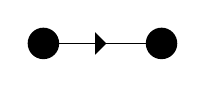
\begin{tikzpicture}
        \fill [black] (0,0) circle (0.2 cm);
        \draw (0,0) -- node {\midarrow} (1.5,0);
        \fill[black] (1.5,0) circle (0.2cm);
        \end{tikzpicture}
    \end{gathered}+
    \begin{gathered}
        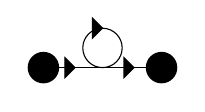
\begin{tikzpicture}
        \fill [black] (0,0) circle (0.2 cm);
        \draw (0,0) -- (1.5,0);
        \fill[black] (1.5,0) circle (0.2cm);
        \draw (0.75,0.25) circle (0.25 cm);
        \draw[-triangle 90] (0.4,0) -- (0.41,0);
        \draw[-triangle 90] (1.15,0) -- (1.16,0);
        \draw[-triangle 90] (0.75,0.5) -- (0.76,0.5);
        \end{tikzpicture}
    \end{gathered}+
    \begin{gathered}
        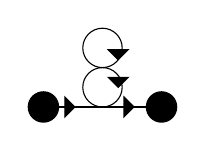
\begin{tikzpicture}
        \fill [black] (0,0) circle (0.2 cm);
        \draw (0,0) -- (1.5,0);
        \fill[black] (1.5,0) circle (0.2cm);
        \draw (0.75,0.25) circle (0.25 cm);
        \draw (0.75,0.75) circle (0.25 cm);
        \draw[-triangle 90] (0.4,0) -- (0.41,0);
        \draw[-triangle 90] (1.15,0) -- (1.16,0);
        \draw[-triangle 90] (0.95,0.25) -- (0.95,0.24);
        \draw[-triangle 90] (0.95,0.6) -- (0.95,0.59);
        \end{tikzpicture}
    \end{gathered}+
    \begin{gathered}
        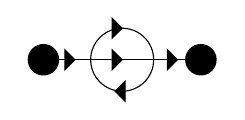
\begin{tikzpicture}
        \fill [black] (0,0) circle (0.2 cm);
        \draw (0,0) -- (2,0);
        \fill[black] (2,0) circle (0.2cm);
        \draw (1,0) circle (0.4 cm);
        \draw[-triangle 90] (0.4,0) -- (0.41,0);
        \draw[-triangle 90] (1.7,0) -- (1.71,0);
        \draw[-triangle 90] (1.,0) -- (1.01,0);
        \draw[-triangle 90] (1.,0.4) -- (1.01,0.4);
        \draw[-triangle 90] (1.,-0.4) -- (0.9,-0.4);
        \end{tikzpicture}
    \end{gathered}\\
    &+\begin{gathered}
        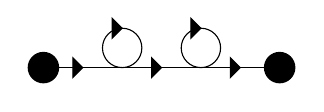
\begin{tikzpicture}
        \fill [black] (0,0) circle (0.2 cm);
        \draw (0,0) -- (3,0);
        \fill[black] (3,0) circle (0.2cm);
        \draw (1,0.25) circle (0.25 cm);
        \draw (2,0.25) circle (0.25 cm);
        \draw[-triangle 90] (0.5,0)--(0.51,0);
        \draw[-triangle 90] (1.5,0)--(1.51,0);
        \draw[-triangle 90] (2.5,0)--(2.51,0);
        \draw[-triangle 90] (1,0.5)--(1.01,0.5);
        \draw[-triangle 90] (2,0.5)--(2.01,0.5);
        \end{tikzpicture}
    \end{gathered}+
    \begin{gathered}
        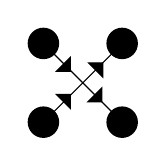
\begin{tikzpicture}
        \fill [black] (-0.5,-0.5) circle (0.2 cm);
        \fill [black] (-0.5,0.5) circle (0.2 cm);
        \fill [black] (0.5,0.5) circle (0.2 cm);
        \fill [black] (0.5,-0.5) circle (0.2 cm);
        \draw (-0.5,-0.5) -- (0.5,0.5);
        \draw (-0.5,0.5) -- (0.5,-0.5);
        \draw[-triangle 90] (0.25,0.25)--(0.26,0.26);
        \draw[-triangle 90] (-0.16,0.15)--(-0.15,0.14);
        \draw[-triangle 90] (-0.16,-0.15)--(-0.15,-0.14);
        \draw[-triangle 90] (0.15,-0.15)--(0.25,-0.25);
        \end{tikzpicture}
    \end{gathered}+
    \begin{gathered}
        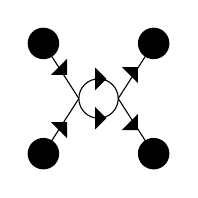
\begin{tikzpicture}
        \fill [black] (-0.7,-0.7) circle (0.2 cm);
        \fill [black] (-0.7,0.7) circle (0.2 cm);
        \fill [black] (0.7,0.7) circle (0.2 cm);
        \fill [black] (0.7,-0.7) circle (0.2 cm);
        \draw (0,0) circle (0.25 cm);
        \draw (-0.7,-0.7) -- (-0.25,0);
        \draw (-0.7,0.7) -- (-0.25,0);
        \draw (0.7,0.7) -- (0.25,0);
        \draw (0.7,-0.7) -- (0.25,0);
        \draw[-triangle 90] (-0.5,0.4)--(-0.4,0.3);
        \draw[-triangle 90] (-0.5,-0.4)--(-0.4,-0.3);
        \draw[-triangle 90] (0.4,0.3)--(0.5,0.4);
        \draw[-triangle 90] (0.4,-0.3)--(0.5,-0.4);
        \draw[-triangle 90] (0,0.25) -- (0.1,0.25);
        \draw[-triangle 90] (0,-0.25) -- (0.1,-0.25);
        \end{tikzpicture}
    \end{gathered}+
        \begin{gathered}
        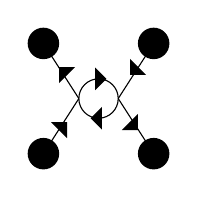
\begin{tikzpicture}
        \fill [black] (-0.7,-0.7) circle (0.2 cm);
        \fill [black] (-0.7,0.7) circle (0.2 cm);
        \fill [black] (0.7,0.7) circle (0.2 cm);
        \fill [black] (0.7,-0.7) circle (0.2 cm);
        \draw (0,0) circle (0.25 cm);
        \draw (-0.7,-0.7) -- (-0.25,0);
        \draw (-0.7,0.7) -- (-0.25,0);
        \draw (0.7,0.7) -- (0.25,0);
        \draw (0.7,-0.7) -- (0.25,0);
        \draw[-triangle 90] (-0.4,0.3)--(-0.5,0.4);
        \draw[-triangle 90] (-0.5,-0.4)--(-0.4,-0.3);
        \draw[-triangle 90] (0.5,0.4)--(0.4,0.3);
        \draw[-triangle 90] (0.4,-0.3)--(0.5,-0.4);
        \draw[-triangle 90] (0,0.25) -- (0.1,0.25);
        \draw[-triangle 90] (0,-0.25) -- (-0.1,-0.25);
        \end{tikzpicture}
    \end{gathered}+\\
    &\begin{gathered}
        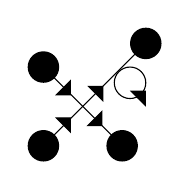
\begin{tikzpicture}
        \fill [black] (-0.5,-0.5) circle (0.2 cm);
        \fill [black] (-0.5,0.5) circle (0.2 cm);
        \fill [black] (0.8,0.8) circle (0.2 cm);
        \fill [black] (0.5,-0.5) circle (0.2 cm);
        \draw (-0.5,-0.5) -- (0.8,0.8);
        \draw (-0.5,0.5) -- (0.5,-0.5);
        \draw (0.6,0.3) circle (0.2 cm);
        \draw[-triangle 90] (0.25,0.25)--(0.26,0.26);
        \draw[-triangle 90] (-0.16,0.15)--(-0.15,0.14);
        \draw[-triangle 90] (-0.16,-0.15)--(-0.15,-0.14);
        \draw[-triangle 90] (0.15,-0.15)--(0.25,-0.25); 
        \draw[-triangle 90] (0.7,0.1)--(0.8,0.2); 
        \end{tikzpicture}
    \end{gathered}
    +\begin{gathered}
        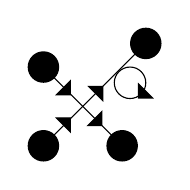
\begin{tikzpicture}
        \fill [black] (-0.5,-0.5) circle (0.2 cm);
        \fill [black] (-0.5,0.5) circle (0.2 cm);
        \fill [black] (0.8,0.8) circle (0.2 cm);
        \fill [black] (0.5,-0.5) circle (0.2 cm);
        \draw (-0.5,-0.5) -- (0.8,0.8);
        \draw (-0.5,0.5) -- (0.5,-0.5);
        \draw (0.6,0.3) circle (0.2 cm);
        \draw[-triangle 90] (0.25,0.25)--(0.26,0.26);
        \draw[-triangle 90] (-0.16,0.15)--(-0.15,0.14);
        \draw[-triangle 90] (-0.16,-0.15)--(-0.15,-0.14);
        \draw[-triangle 90] (0.15,-0.15)--(0.25,-0.25); 
        \draw[-triangle 90] (0.8,0.2)--(0.7,0.1); 
        \end{tikzpicture}
    \end{gathered}+\order{\lambda^3}
    \end{aligned}
    \label{W_phi4_complex}
\end{equation}
\chapter{Scattering Amplitudes}
In this chapter we derive Feynman's Rules for calculating scattering amplitudes in $\phi^3$ theory. Now that we know that $Z(J)=\exp i W(J)$ we can start to calculate correlation functions and get information from them. For instance, we can check for consistency by evaluating the familar result
\begin{equation}
    \frac{1}{i}\Delta(x_1-x_2)=\vev{\text{T}\phi(x_1)\phi(x_2)}.
\end{equation}
To clear the notation, we introduce $\delta_j=\frac{1}{i}\fdv{J(x_j)}$. Calculating the derivatives, recalling that $Z(0)=1$, gives
\begin{equation}
\begin{aligned}
     \vev{\text{T}\phi(x_1)\phi(x_2)}&= \delta_1\delta_2Z(J)\eval_{J=0}\\
     &=\delta_1[Z(J)\delta_2iW(J)]\eval_{J=0}\\
     &=\delta_1Z(J)\eval_{J=0}\delta_2 iW(J)\eval_{J=0}+Z(J)\delta_1\delta_2iW(J)\eval_{J=0}\\
     &=\delta_1iW(J)\eval_{J=0}\delta_2 iW(J)\eval_{J=0} + \delta_1\delta_2iW(J)\eval_{J=0}.
\end{aligned}
\end{equation}
Since $\delta_jiW(J)\eval_{J=0}=\vev{\phi(x_j)}=0$, then
\begin{equation}
    \vev{\text{T}\phi(x_1)\phi(x_2)}=\delta_1\delta_2iW(J)\eval_{J=0}
\end{equation}
which is the sum of connected diagrams with two sources, but with the two sources removed:
\begin{equation}
    \vev{\text{T}\phi(x_1)\phi(x_2)}=
    \begin{gathered}
       \begin{tikzpicture}
     \draw (0,0) -- (1,0.0);
    \end{tikzpicture}
    \end{gathered}
    +
     \begin{gathered}
       \begin{tikzpicture}
     \draw (0,0) -- (1,0);
     \draw (1.5,0) circle(0.5);
     \draw (2,0) -- (3,0);
    \end{tikzpicture}
    \end{gathered}
    +\order{g^4}
    % \begin{gathered}
     %  \begin{tikzpicture}
     %\draw (0,0) -- (1,0);
     %\draw (1.5,0) circle(0.5);
     %\draw (2,0) -- (3,0);
     %\draw (1.5,-0.5) -- (1.5,0.5);
    %\end{tikzpicture}
    %\end{gathered}
    \label{nao_conectados}
\end{equation}
Which agrees, up to $\order{g^2}$, with what we expected: $\vev{\text{T}\phi(x_1)\phi(x_2)}=\frac{1}{i}\Delta(x_1-x_2)$.\\

We now focus on the object we are most interested in, since it goes into the LSZ formula, the four-point correlation:
\begin{equation}
    \vev{\text{T}\phi(x_1)\phi(x_2)\phi(x_3)\phi(x_4)}=\delta_1\delta_2\delta_3\delta_4 Z(J)\eval_{J=0},
\end{equation}
for which the result is
\begin{equation}
\begin{aligned}
     \vev{\text{T}\phi(x_1)\phi(x_2)\phi(x_3)\phi(x_4)}&=\frac{1}{i}\Delta(x_{1^\prime}-x_2)\frac{1}{i}\Delta(x_{1}-x_{2^\prime})\\&+\frac{1}{i}\Delta(x_{1}-x_2)\frac{1}{i}\Delta(x_{1^\prime}-x_{2^\prime})\\&+\frac{1}{i}\Delta(x_1-x_{1^\prime})\frac{1}{i}\Delta(x_2-x_{2^\prime})\\&+\delta_1\delta_2\delta_3\delta_4 i W(J).
     \label{4pointW}
\end{aligned}
\end{equation}
We argue that only the last term is of any interest for scattering. Let's see why. Plugging any of the  terms consisting of products of propagators into the LSZ, say, the term in the next-to-last line in (\ref{4pointW}), we get
\begin{equation}
    \begin{aligned}
    &i^2\int\dd^4x_1\dd^4x_2\dd^4x_{1^\prime}\dd^4x_{2^\prime}e^{i(k_1x_1+k_2x_2-k^\prime_1x_{1^\prime}-k_{2}^\prime x_{2^\prime}})&\\&\times(-\partial_1^2+m^2)(-\partial_{1^\prime}^2+m^2)\Delta(x_1-x_{1^\prime})(-\partial_2^2+m^2)(-\partial^2_{2^\prime}+m^2)\Delta(x_2-x_{2^\prime}).
    \end{aligned}
    \label{produtoLSZ}
\end{equation}
Working on the first pair of Klein-Gordon differential operators (the other is completely analogous), we define the function $F(x_1-x_{1^\prime})=(-\partial_1^2+m^2)(-\partial_{1^\prime}^2+m^2)\Delta(x_1-x_{1^\prime})$. The product in (\ref{produtoLSZ}) involving this function and the variables it depends on is
\begin{equation}
    \int\dd^4x_1\dd^4x_{1^\prime}e^{i(k_1x_1-k^\prime_1x_{1^\prime})}F(x_1-x_{1^\prime}).
    \label{termoF}
\end{equation}
We change variables to $y=x_1-x_{1^\prime}$ and $z=\frac{1}{2}(x_1+x_{1^\prime})$, so that (\ref{termoF}) reads
\begin{equation}
    \int\abs{\pdv{(x_1,x_{1^\prime})}{(y,z)}}\dd^4y\,\dd^4z\,e^{i(k_1+k_1^\prime)y/2}e^{i(k_1-k_1^\prime)z}F(y)
\end{equation}
since the jacobian for such transformation of variables is $1$, we see that 
\begin{equation}
    \int\dd^4x_1\dd^4x_{1^\prime}e^{i(k_1x_1-k^\prime_1x_{1^\prime})}F(x_1-x_{1^\prime})
    =(2\pi)^4\delta^4(k_1-k_1^\prime)\widetilde{F}(\Bar{k}_{11})
\end{equation}
where $\widetilde{F}(\Bar{k}_{11})$ is the Fourier transform of $F(y)$ and $\bar{k}_{ij}=\frac{1}{2}(k_i+k_j^\prime)$.
Therefore, (\ref{produtoLSZ}) gives the following contribution to the amplitude
\begin{equation}
\braket{f}{i}=i^2(2\pi)^4\delta^4(k_1-k_{1^\prime})(2\pi)^4\delta^4(k_2-k_{2^\prime})\widetilde{F}(\bar{k}_{11})\widetilde{F}(\bar{k}_{22})
\end{equation}
which is a selection rule for processes in which the 4-momentum of the particles do not change in transitioning from the in and out states: they do not correspond to a scattering. We conclude then that terms involving the product of propagators in (\ref{4pointW}) do not contribute to scattering, either because of what we just presented or because they vanish, since some of them can involve $\delta^4(k_1+k_2)$ or $\delta^4(k_1^\prime+k_2^\prime)$. As a result, since the sum of energies is always positive, i.e. $k_1^0+k_2^0\geq2m>0$, we never reach the ``peak" of the Delta distribution: integrals involving these Deltas vanish.\\

Therefore, products of diagrams such as the ones in (\ref{nao_conectados}) do not contribute to scattering amplitudes. 
%The only term contributing is the last one in (\ref{4pointW})), which corresponds to the sum of connected diagrams with four sources, with those sources removed, that is ().
This motivates the definition of a \textit{fully connected correlation function} as the term that actually contributes to scattering
\begin{equation}
    \vev{\text{T}\phi(x_1)\dots\phi(x_E)}_{\text{C}}=\delta_1\delta_2\dots\delta_EiW(J)\eval_{J=0}.
\end{equation}
The term we are interested in, $\delta_1\delta_2\delta_3\delta_4 i W(J)$, when $J=0$, corresponds to the sum of diagrams with four sources, but with them removed. Up to $g^2$, we highlight the diagram of interest in (\ref{iWphi3}).
\begin{equation}
iW(J)=\dots+
\begin{gathered}
              \begin{tikzpicture}
                \fill[black] (1,1) circle (0.3 cm);
                 \fill[black] (-1,1) circle (0.3 cm);
                 \fill[black] (-1,-1) circle (0.3cm);
                 \fill[black] (1,-1) circle (0.3 cm);
                 \draw (-0.5,0) -- (0.5,0);
                 \draw (-1,1) -- (-0.5,0);
                 \draw (1,1) -- (0.5,0);
                 \draw (-1,-1) -- (-0.5,0);
                 \draw (1,-1) -- (0.5,0);
            \end{tikzpicture}
\end{gathered}+\order{g^4}
\label{tree_sources}
\end{equation}
This diagram with its sources removed will consist of different arrangements of labels $x_i$, due to the possible actions of the functional derivatives. There are $4!$ of such arrangements and they are exactly eight copies of the same three diagrams below, called \textit{tree diagrams}
\begin{equation}
\delta_1\delta_2\delta_3\delta_4 i W(J)=
\begin{gathered}
    \begin{tikzpicture}
     \feynmandiagram [small,horizontal=a to b] {
      i1 [particle=\(x_2\)] --  a --  i2 [particle=\(x_1\)],
      a --  b,
      f1 [particle=\(x_{2^\prime}\)] --  b --  f2 [particle=\(x_{1^\prime}\)],
    };
    \end{tikzpicture}
\end{gathered}+
\begin{gathered}
    \feynmandiagram [small,vertical=a to b] {
      i1 [particle=\(x_1\)] --  a --  i2 [particle=\(x_{1^\prime}\)],
      a --  b,
      f1 [particle=\(x_2\)] --  b --  f2 [particle=\(x_{2^\prime}\)],
    };
\end{gathered}+
\begin{gathered}
   \feynmandiagram [small,vertical=a to b] {
      i1 [particle=\(x_1\)] --  a --  i2 [particle=\(x_{2^\prime}\)],
      a --  b,
      f1 [particle=\(x_2\)] --  b --  f2 [particle=\(x_{1^\prime}\)],
    };
\end{gathered} +\order{g^4}
\label{trees}
\end{equation}
Since the diagram highlighted in (\ref{tree_sources}) has symmetry factor $S=8$, the eight copies of the three configurations cancel the symmetry factor. Tree-diagrams thus have this property: after removing the sources, we get $S=1$ for their symmetry factor. Translating (\ref{trees}) we find
\begin{equation}
\begin{aligned}
  \vev{\text{T}\phi(x_1)\phi(x_2)\phi(x_1^\prime)\phi(x_2^\prime)}_{\text{C}}&=(ig)^2\qty(\frac{1}{i})^5\int\dd^4 y\,\dd^4 z\, \Delta(y-z)\\
  &\times[\Delta(x_1-y)\Delta(x_2-y)\Delta(x_{1^\prime}-z)\Delta(x_{2^\prime}-z)\\
  &+\Delta(x_1-y)\Delta(x_{1^\prime}-y)\Delta(x_2-z)\Delta(x_{2^\prime}-z)\\
  &+\Delta(x_1-y)\Delta(x_{2^\prime}-y)\Delta(x_2-z)\Delta(x_{1^\prime}-z)]+\order{g^4}
\end{aligned}
\end{equation}
Plugging in the LSZ, bearing in mind that the propagator $\Delta(x-y)$ is the Green's Function for the Klein-Gordon differential operator $(-\partial^2+m^2)$, we have
\begin{equation}
\begin{aligned}
   \braket{f}{i}&=i^4\int\dd^4x_1\dd^4x_2\dd^4x_{1^\prime}\dd^4x_{2^\prime}\,e^{ik_1x_1}e^{ik_2x_2}e^{-ik_{1}^\prime x_{1^\prime}}e^{-ik_{2}^\prime x_{2^\prime}}\\&\qquad\quad\times(-\partial_1^2+m^2)(-\partial_2^2+m^2)
    \,(-\partial_{1^\prime}^2+m^2)(-\partial_{2^\prime}^2+m^2)\\&\qquad\quad\times\bra{0}\text{T}\phi(x_1)\phi(x_2)\phi(x_{1^\prime})\phi(x_{2^\prime})\ket{0}_{\text{C}}\\
    &=(ig)^2\frac{1}{i}\int\dd^4y\,\dd^4z\,\dd^4x_1\,\dd^4x_2\,\dd^4x_{1^\prime}\,\dd^4x_{2^\prime}\, e^{i(k_1x_1+k_2x_2-k_1^\prime x_{1^\prime} - k_2^\prime x_{2^\prime})}\Delta(y-z)\\
    &\qquad\quad\times\Big{[}\delta^4(x_1-y)\delta^4(x_2-y)\delta^4(x_{1^\prime}-z)\delta^4(x_{2^\prime}-z)\\
  &\qquad\quad+\delta^4(x_1-y)\delta^4(x_{1^\prime}-y)\delta^4(x_2-z)\delta^4(x_{2^\prime}-z)\\
  &\qquad\quad+\delta^4(x_1-y)\delta^4(x_{2^\prime}-y)\delta^4(x_2-z)\delta^4(x_{1^\prime}-z)\Big{]}+\order{g^4}\\
  &=ig^2\int\dd^4y\,\dd^4z\,\Delta(y-z)\Big{[}e^{i(k_1y+k_2y-k_1^\prime z -k_2^\prime z)}+e^{i(k_1y+k_2z-k_1^\prime y -k_2^\prime z)}  \\&\qquad\quad + e^{i(k_1y+k_2z-k_1^\prime z - k_2^\prime y)}\Big{]}+\order{g^4}.
\end{aligned}
\end{equation}
We use the definition of the propagator
\begin{equation}
    \Delta(y-z)=\int\frac{\dd ^4 k}{(2\pi)^4}\frac{e^{ik(y-z)}}{k^2+m^2-i\epsilon}
\end{equation}
and the Dirac Delta 
\begin{equation}
    \delta^4(w-v)=\int\frac{\dd^4 k}{(2\pi)^4}e^{i(w-v)k}
\end{equation}
so the amplitude reads
\begin{equation}
\begin{aligned}
   \braket{f}{i}=&ig^2\int\frac{\dd^4 k}{(2\pi)^4}\frac{1}{k^2+m^2-i\epsilon}\Big{[}(2\pi)^4\delta^4(k_1+k_2+k)(2\pi)^4\delta^4(k_1^\prime+k_2^\prime+k)\\
   &+(2\pi)^4\delta^4(k_1-k_1^\prime+k)(2\pi)^4\delta^4(k_2^\prime-k_2+k)\\&+(2\pi)^4\delta^4(k_1-k_2^\prime+k)(2\pi)^4\delta^4(k_1^\prime-k_2+k)\Big{]}+\order{g^4}
\end{aligned}
\end{equation}
and we finally arrive at
\begin{equation}
\begin{aligned}
    \braket{f}{i}=&ig^2(2\pi)^4\delta^4(k_1+k_2-k_1^\prime-k_2^\prime)\\
    &\times\qty[\frac{1}{(k_1+k_2)^2+m^2}+\frac{1}{(k_1-k_1^\prime)^2+m^2}+\frac{1}{(k_1-k_2^\prime)^2+m^2}]+\order{g^4}
    \label{fi_final},
\end{aligned}
\end{equation}
where we dropped the $i\epsilon$s since the denominators cannot vanish for physically allowed values of momenta. This result can be generalized as
\begin{equation}
    \braket{f}{i}=(2\pi)^4\delta^4(k_{\text{in}}-k_{\text{out}})i\mathcal{T}
    \label{scattering_amplitude}
\end{equation}
in which the $i\mathcal{T}$ will be determined according to \textit{Feynman's Rules}. These rules allow us to translate diagrams directly into scattering amplitudes, without repeating  the previous calculations we have done.
The Feynman Rules for $\phi^3$ theory are
\begin{itemize}
    \item We draw lines for incoming and outgoing particles. Time runs from left to right.
    \item One side of these incoming and outgoing lines must be free while the other must be joined to a \textit{vertex}. A vertex must join three lines. We must draw all the \textit{topologically nonequivalent} diagrams: those that cannot be transformed into another one by deformations.
    \item For each incoming line, draw an arrow pointing toward the vertex; for each outgoing line draw an arrow pointing outward the vertex; for internal lines draw an arrow with arbitrary direction.
    \item To each line, associate a 4-momentum. To external lines, this 4-momentum should be that of the particle the line represents
    \item Think of 4-momentum as a fluid flowing through the diagram and demand its conservation at the vertices.
    \item When translating into scattering amplitudes, external lines equals to $1$.
    \item Internal lines with 4-momentum $k$ correspond to $\frac{-i}{k^2+m^2-i\epsilon}$
    \item Vertices correspond to $iZ_gg$.
\end{itemize}
This way,  result (\ref{fi_final}) we found can be stated as (\ref{scattering_amplitude}) where
\begin{equation}
    i\mathcal{T}=
    \begin{gathered}
       \feynmandiagram [medium,horizontal=a to b] {
      i1 [particle=\(k_2\)] -- [fermion]  a -- [anti fermion] i2 [particle=\(k_1\)],
      a -- [momentum=\(k_1+k_2\)] b,
      f1 [particle=\(k_{1}^\prime\)] -- [anti fermion]  b -- [fermion]  f2 [particle=\(k_{2}^\prime\)],
    };
    \end{gathered}+
    \begin{gathered}
       \feynmandiagram [medium,vertical=a to b] {
      i1 [particle=\(k_1\)] -- [fermion]  a -- [fermion] i2 [particle=\(k_1^\prime\)],
      a -- [momentum=\(k_1-k_1^\prime\)] b,
      f1 [particle=\(k_{2}^\prime\)] -- [anti fermion]  b -- [anti fermion]  f2 [particle=\(k_{2}\)],
    };
    \end{gathered}+
    \begin{gathered}
       \feynmandiagram [medium,vertical=a to b] {
      i1 [particle=\(k_1\)] -- [fermion]  a -- [fermion] i2 [particle=\(k_2^\prime\)],
      a -- [momentum=\(k_1-k_2^\prime\)] b,
      f1 [particle=\(k_{1}^\prime\)] -- [anti fermion]  b -- [anti fermion]  f2 [particle=\(k_{2}\)],
    };
    \end{gathered}
\end{equation}


\chapter{Observables: Cross-sections and decay rates}
From scattering amplitudes we will obtain the most common observables of interest in high-energies: the cross-section and the decay rate. The first will contain information about the probability of collisions and the second will contain information about the probability of transmutation of one type of particle to another one or to a set of different particles.
\section{High-energy collisions in the Lab and CM frames}
We examine collisions in two different frames of reference. The first we consider is that lying in the center of mass (CM) of a two-particle system. Suppose we have two particles heading toward one another along the $z$ axis. We label their masses $m_1$ and $m_2$, their 3-momenta $\vb{k}_1$ and $\vb{k}_2$, and 4-momenta $k_1$ and $k_2$, normalized as $k_i^2=-m^2_i$. In this setup, the total 3-momentum vanishes: $\vb{k}_1+\vb{k}_2=0$. We define the invariant $s=-(k_1+k_2)^2$, which in the CM frame reduces to $s=(E_1+E_2)^2$. Bearing in mind the mass-shell relations
\begin{equation}
    \begin{aligned}
        E_1&=\sqrt{\vb{k}_1^2+m_1^2}\\
        E_2&=\sqrt{\vb{k}_2^2+m_2^2}
    \end{aligned}
\end{equation}
and that $\vb{k}_2=-\vb{k}_1$, then we can show that
\begin{equation}
    \abs{\vb{k}_1}=\frac{1}{2\sqrt{s}}\sqrt{s^2-2(m_1^2+m_2^2)s+(m_1^2-m_2^2)^2}.
    \label{k1}
\end{equation}
After the collision, in the CM frame we again have $\vb{k}_1^\prime+\vb{k}_2^\prime=0$ and $(E_1^\prime+E_2^\prime)^2=s$, so that
\begin{equation}
    \abs{\vb{k}_1^\prime}=\frac{1}{2\sqrt{s}}\sqrt{s^2-2(m_{1^\prime}^2+m_{2^\prime}^2)s+(m_{1^\prime}^2-m_{2^\prime}^2)^2}.
    \label{k1linha}
\end{equation}
To specify the angle $\theta$ between $\vb{k}_1$ and $\vb{k}_1^\prime$, we define another invariant $t=-(k_1-k_1^\prime)^2$
\begin{equation}
    t=m_1^2+m_{1^\prime}^2-2E_1E_{1^\prime}+2\abs{\vb{k}_1}\abs{\vb{k}_{1}^\prime}\cos\theta
    \label{tzinho}
\end{equation}
valid in any frame. The scalars $s$ and $t$ are two of the \textit{Mandelstam Variables}, defined by
\begin{equation}
    \begin{aligned}
        s=-(k_1+k_2)^2&=-(k_{1^\prime}+k_{2^\prime})^2\\
        t=-(k_1-k_{1^\prime})^2&=-(k_2-k_{2^\prime})^2\\
        u=-(k_1-k_{2^\prime})^2&=-(k_2-k_{1^\prime})^2
    \end{aligned}
    \label{mandelstam}
\end{equation}
and satisfying
\begin{equation}
    s+t+u=m_1^2+m_2^2+m_{1^\prime}^2+m_{2^\prime}^2.
    \label{soma_mandelstam}
\end{equation}
In terms of Mandelstam variables, the scattering amplitude we found in last section reads
\begin{equation}
    i\mathcal{T}=ig^2\qty[\frac{1}{m^2-s}+\frac{1}{m^2-t}+\frac{1}{m^2-u}].
\end{equation}

Now we consider a fixed target frame (FT), ie. the lab frame. A particle lies at rest $\vb{k_2}=0$ while the other hits it with 3-momentum $\vb{k}_1$ along a $z$ axis. In this case we can check that
\begin{equation}
    \abs{\vb{k}_1}=\frac{1}{2m_2}\sqrt{s^2-2(m_1^2+m_2^2)s+(m_1^2-m_2^2)^2}.
\end{equation}
That is, $m_2\abs{\vb{k}_1}_{\text{FT}}=\sqrt{s}\abs{\vb{k}_1}_{\text{CM}}$.
\section{The differential cross-section}
To get information about the probability of a scattering event between two incoming particles resulting in $n^\prime$ outgoing particles, we look for the \textit{cross-section}: a parameter with dimensions of area specifying the probability of a scattering event given the knowledge of the number of incoming particles and their velocities. \\

From the amplitude (\ref{scattering_amplitude}) we can construct first the \textit{differential cross-section}, which gives the total cross-section upon integration. To this end, we consider a system of particles enclosed in a large cubical box of sides $L$ and volume $V=L^3$, with the scattering event happening during an interval $T$ of time. Considering the amplitude (\ref{scattering_amplitude}), the probability of scattering is
\begin{equation}
    P=\frac{\abs{\braket{f}{i}}^2}{\braket{f}\braket{i}}.
\end{equation}
Now, since
\begin{equation}
    \abs{\braket{f}{i}}^2=(2\pi)^4\delta^4(k_{\text{in}}-k_{\text{out}})(2\pi)^4\delta^4(0)\abs{\mathcal{T}}^2
\end{equation}
and noting that
\begin{equation}
    (2\pi)^4\delta^4(0)=\int\dd^4x\, e^{i0x}=VT
\end{equation}
and that the initial and final states are normalized as $\braket{k}=(2\pi)^32k^0\delta^3(\vb{0})=2k^0V$, then we can see that for the incoming two-particle state we have
\begin{equation}
    \braket{i}=4E_1E_2V^2
\end{equation}
and for the $n^\prime$ outgoing ones 
\begin{equation}
    \braket{f}=\prod_{j=1}^{n^\prime}2k^{\prime0}_{j} V.
\end{equation}
Then, the scattering probability per unit time reads
\begin{equation}
    \dot{P}=\frac{(2\pi)^4\delta^4(k_{\text{in}}-k_{\text{out}})V\abs{\mathcal{T}}^2}{4E_1E_2V^2\prod_{j=1}^{n^\prime}2k_j^{\prime0}V}.
\end{equation}
We must sum over the momenta of outgoing particles $\vb{k}^\prime_j$. Imposing periodic boundary conditions to the box enclosing the system, momentum states will be discrete: $\vb{k}^\prime_j=\frac{2\pi}{L}\vb{n}_j^\prime$, with $\vb{n}_j^\prime$ being a vector with integer entries. In the limit $L\to\infty$, we replace the sum for an integral: $\sum_{\vb{n}_j^\prime}\to\frac{V}{(2\pi)^3}\int\dd^3k^\prime_j$. Therefore, the probability per unit time must be multiplied by the appropriate factor $\frac{V}{(2\pi)^3}\dd^3k^\prime_j$ for each outgoing particle so that it gives the correct answer upon integration (summation). That is
\begin{equation}
    \dot{P}=\frac{(2\pi)^4\delta^4(k_{\text{in}}-k_{\text{out}})\abs{\mathcal{T}}^2}{4E_1E_2V}\prod_{j=1}^{n^\prime}\widetilde{\dd k}^\prime_j
\end{equation}
where $\widetilde{\dd k}_j^\prime=\frac{\dd^3 k_{j}^\prime}{(2\pi)^32k^{\prime0}_j}$ is the Lorentz invariant measure. \\

The cross-section $\sigma$  expresses the proportionality between the number of observed scattering events and the incident flux of particles $J$. The differential cross-section $\dd \sigma$ is then equal to $\dot{P}/J$. The flux $J$ is the number of incoming particles per volume times their speed. Considering a single incoming particle with $E_1=m_1\gamma$, $\vb{k}_1=m_1\gamma\vb{v}_1$, in the FT frame with the second particle at rest, the incident flux is $\frac{1}{V}v=\frac{\abs{\vb{k}_1}}{E_1V}$, since there is only one particle and $v=\frac{\abs{\vb{k}_1}}{E_1}$ is its velocity. The differential cross-section $\dd\sigma=\frac{\dot{P}}{\abs{\vb{k}_1}/E_1V}$ reads
\begin{equation}
    \dd \sigma=\frac{(2\pi)^4\delta^4(k_{\text{in}}-k_{\text{out}})\abs{\mathcal{T}}^2}{4\abs{\vb{k}_1}E_2}\prod_{j=1}^{n^\prime}\widetilde{\dd k}^\prime_j.
\end{equation}
Recalling that, in the FT frame $E_2=m_2$, and that $\abs{\vb{k}_1}=\abs{\vb{k}_1}_{\text{FT}}=\frac{\sqrt{s}}{m_2}\abs{\vb{k}_1}_{\text{CM}}$, defining a Lorentz invariant phase-space integration measure for $n^\prime$ outgoing particle scattering by
\begin{equation}
    \dd \text{LIPS}_{n^\prime}(k)=(2\pi)^4\delta^4\qty(k-\sum_{i=1}^{n^\prime}k_i^\prime)\prod_{j=1}^{n^\prime}\widetilde{\dd k}_j^\prime
\end{equation}
then the differential cross-section reads
\begin{equation}
    \dd \sigma=\frac{1}{4\abs{\vb{k}_1}_{\text{CM}}\sqrt{s}}\abs{\mathcal{T}}^2\dd \text{LIPS}_{n^\prime}(k_1+k_2).
\end{equation}
For the special case of two outgoing particles in the CM frame: $\dd \text{LIPS}_{2}(k_1+k_2)=(2\pi)^4\delta^4(k_1+k_2-k_1^\prime-k_2^\prime)\widetilde{\dd k}_1^\prime\widetilde{\dd k}_2^\prime$, $\vb{k}_1+\vb{k}_2=0$ and $k^0_1+k^0_2=E_1+E_2=\sqrt{s}$ so 
\begin{equation}
    \begin{aligned}
        \dd \text{LIPS}_{2}(k_1+k_2)&=(2\pi)^4\delta(E_1^\prime+E_2^\prime-\sqrt{s})\delta^3(\vb{k}_1^\prime+\vb{k}_2^\prime)\frac{\dd^3k_1^\prime}{(2\pi)^32E_1^\prime}\frac{\dd^3k_2^\prime}{(2\pi)^32E_2^\prime}\\
        &=\frac{1}{4(2\pi)^2E_1^\prime E_2^\prime}\delta(E_1^\prime+E_2^\prime-\sqrt{s})\delta^3(\vb{k}_1^\prime+\vb{k}_2^\prime)\dd^3k_1^\prime\dd^3k_2^\prime.
    \end{aligned}
\end{equation}
Integration over $\dd^3 k_2^\prime$ sets $\vb{k}_2^\prime=-\vb{k}_1^\prime$ and $E_2^\prime=\sqrt{\vb{k}_1^{\prime2}+m_{2^\prime}^2}$. We change to spherical coordinates: $\dd^3k_1^\prime=\abs{\vb{k}_1^\prime}^2\dd \abs{\vb{k}_1^\prime}\dd \Omega_{\text{CM}}$, where $\dd\Omega_{\text{CM}}=\sin\theta\dd\theta\dd\phi$ is the solid angle element in the CM frame, $\theta$ being the angle between $\vb{k}_1$ (parallel to $z$) and $\vb{k}_1^\prime$. Next we integrate over $\dd \abs{\vb{k}_1^\prime}$ making use of the property
\begin{equation}
    \delta(f(x))=\sum_{\substack{x_i\\{f(x_i)=0}}}\frac{1}{\abs{f^\prime(x_i)}}\delta(x-x_i)
\end{equation}
being $x_i$ the zeroes of $f(x)$ and $f^\prime(x)$ its derivative. This means
\begin{equation}
    \begin{aligned}
        \int\abs{\vb{k}_1^\prime}^2\dd\abs{\vb{k}_1^\prime}\delta\qty(E_1^\prime+E_2^\prime-\sqrt{s})&=\abs{\vb{k}_1^\prime}^2\abs{\pdv{\abs{\vb{k}_1^\prime}}(E_1^\prime+E_2^\prime-\sqrt{s})}^{-1}\\
        &=\abs{\vb{k}_1^\prime}^2\abs{\frac{\abs{\vb{k}_1^\prime}}{E_1^\prime}+\frac{\abs{\vb{k}_1^\prime}}{E_2^\prime}}^{-1}\\
        &=\abs{\vb{k}_1^\prime}^2\frac{1}{\abs{\vb{k}_1^\prime}}\frac{E_1^\prime E_2^\prime}{E_1^\prime+E_2^\prime}\\
        &=\abs{\vb{k}_1^\prime}\frac{E_1^\prime E_2^\prime}{\sqrt{s}}
    \end{aligned}
\end{equation}
where $\abs{\vb{k}_1^\prime}$ is the solution to $E_1^\prime+E_2^\prime=\sqrt{s}$, given by (\ref{k1linha}). The phase space measure reads 
\begin{equation}
\dd \text{LIPS}_{2}(k_1+k_2)=\frac{\abs{\vb{k}_1^\prime}}{16\pi^2\sqrt{s}}\dd\Omega_{\text{CM}}   
\label{dlips2}
\end{equation}
and so the differential cross-section is
\begin{equation}
    \dv{\sigma}{\Omega_{\text{CM}}}=\frac{1}{64\pi^2s}\frac{\abs{\vb{k}_1^\prime}}{\abs{\vb{k}_1}}\abs{\mathcal{T}}^2
\end{equation}
with $\abs{\vb{k}_1}$ and $\abs{\vb{k}_1^\prime}$ evaluated at the CM frame, where they are given by (\ref{k1}) and (\ref{k1linha}). Also in CM frame, we note that (\ref{tzinho}) gives
\begin{equation}
    \dd t=2\abs{\vb{k}_1}\abs{\vb{k}_1^\prime}\dd \cos \theta=2\abs{\vb{k}_1}\abs{\vb{k}_1^\prime}\frac{\dd \Omega_{\text{CM}}}{2\pi}
\end{equation}
so we can write
\begin{equation}
    \dv{\sigma}{t}=\dv{\sigma}{\Omega_{\text{CM}}}\qty(\dv{t}{\Omega_{\text{CM}}})^{-1}=\frac{1}{64\pi s\abs{\vb{k}_1}^2}\abs{\mathcal{T}}^2
    \label{dsigmadt}
\end{equation}

Now, for the total cross-section $\sigma$, we must integrate the differential cross-section, but there is a subtle detail. If the outgoing particles are identical we must divide by a symmetry factor $S$
\begin{equation}
    \sigma=\frac{1}{S}\int\dd\sigma
\end{equation}
where 
\begin{equation}
    S=\prod_i n_i^\prime!
\end{equation}
This is because if there are identical particles, integration over outgoing momenta will treat them as distinguishable, leading to an over-count. In the case of 2 outgoing particles $S=1$ if the particles are distinguishable and $S=2$ if they are identical. Therefore
\begin{equation}
    \sigma=\frac{1}{S}\int\dv{\sigma}{\Omega_{\text{CM}}}\dd \Omega_{\text{CM}}=\frac{2\pi}{S}\int_{-1}^1\dv{\sigma}{\Omega_{\text{CM}}}\,\dd \cos \theta.
\end{equation}
To evaluate this integral, we must express $t$ and $u$ in terms of $s$ and $\theta$, since the differential cross-section presents dependence on these variables. Alternatively, we can make use of
\begin{equation}
    \sigma=\frac{1}{S}\int_{t_{\text{min}}}^{t_{\text{max}}}\dv{\sigma}{t}\dd t
    \label{total_cross_section}
\end{equation}
and express $u$ in terms of  $s$ and $t$ and integrate over $t$ at fixed $s$. The values of $t_{\text{min}}$ and $t_{\text{max}}$ are given by (\ref{tzinho}), when $\theta=\pi$ , for the minimum, and $\theta=0$, for the maximum.

\section{Cross-sections in $\phi^3$ theory}
We calculate, in $\phi^3$ theory, the cross-section for a scattering involving two incoming particles in the CM frame with equal masses $m$, yielding two outgoing particles. In this setup: $E_1=E_2=E=\sqrt{\vb{k}_1^2+m^2}$; $s=(E_1+E_2)^2=4E^2$; $\abs{\vb{k}_1}=\abs{\vb{k}_1^\prime}=\frac{1}{2}(s-4m^2)^{1/2}$, according to (\ref{k1}) and (\ref{k1linha}); $t=-\frac{1}{2}(s-4m^2)(1-\cos\theta)$, according to (\ref{tzinho}); and $s+t+u=4m^2$, according to (\ref{mandelstam}). So $u=-\frac{1}{2}(s-4m^2)(1+\cos\theta)$. Our task is to expand 
\begin{equation}
    \mathcal{T}=g^2\qty[\frac{1}{m^2-s}+\frac{1}{m^2-t}+\frac{1}{m^2-u}]+\order{g^4}.
\end{equation}
and integrate (\ref{total_cross_section}).\\

First, in the non-relativistic limit, where $\abs{\vb{k}_1}\ll m$, or, equivalently $s-4m^2\ll m^2$, $s\ll m^2$, binomial expansion gives
\begin{equation}
    \frac{1}{m^2-s}\approx\frac{1}{m^2}\qty[1+\frac{s}{m^2}+\frac{s^2}{m^4}\dots]
\end{equation}
\begin{equation}
    \frac{1}{m^2-t}\approx\frac{1}{m^2}\qty[1-\frac{1}{2m^2}(s-4m^2)(1-\cos\theta)+\frac{1}{4m^4}(s-4m^2)^2(1-\cos\theta)^2+\dots]
\end{equation}
\begin{equation}
    \frac{1}{m^2-u}\approx\frac{1}{m^2}\qty[1-\frac{1}{2m^2}(s-4m^2)(1+\cos\theta)+\frac{1}{4m^4}(s-4m^2)^2(1+\cos\theta)^2+\dots]
\end{equation}
Adding the terms and rearranging in powers of $(s-4m^2)/m^2$:
\begin{equation}
    \mathcal{T}=\frac{5g^2}{3m^2}\qty[1-\frac{8}{15}\qty(\frac{s-4m^2}{m^2})+\frac{5}{18}\qty(1+\frac{27}{25}\cos^2\theta)\qty(\frac{s-4m^2}{m^2})^2+\dots]+\order{g^4}
\end{equation}
which gives a nearly isotropic differential cross-section. In the extreme relativistic limit, where $\abs{\vb{k}_1}\gg m$, or, equivalently $s\gg m^2$, expansion in powers of $m^2/s$ gives :
\begin{equation}
\mathcal{T}=\frac{g^{2}}{s \sin ^{2} \theta}\left[3+\cos ^{2} \theta-\left(\frac{\left(3+\cos ^{2} \theta\right)^{2}}{\sin ^{2} \theta}-16\right) \frac{m^{2}}{s}+\ldots\right]+\order{g^4}
\end{equation}
which is peaked in $\theta=0$ and $\theta=\pi$. These results tell us that, in the non-relativistic limit, scatterings are equally likely in any direction while, in the relativistic limit, particles are more likely to scatter along the direction of the incident particle.\\

We can integrate (\ref{total_cross_section}) using (\ref{dsigmadt}). In this case $t_{\text{min}}=-(s-4m^2)$ and $t_{\text{max}}=0$. We are considering identical particles so $S=2$. The relation among Mandelstam variables gives $u=4m^2-s-t$. Integration over $t$ with fixed $s$ gives
\begin{equation}
\begin{aligned}
\sigma=&\frac{g^{4}}{32 \pi s\left(s-4 m^{2}\right)}\left[\frac{2}{m^{2}}+\frac{s-4 m^{2}}{\left(s-m^{2}\right)^{2}}-\frac{2}{s-3 m^{2}}\right.
\\
&\left.\qquad\qquad\qquad\qquad+\frac{4 m^{2}}{\left(s-m^{2}\right)\left(s-2 m^{2}\right)} \ln \left(\frac{s-3 m^{2}}{m^{2}}\right)\right]  
\end{aligned}{}
\end{equation}
\section{Decay rates}
Even though the LSZ formula demands incoming and outgoing states to be single-particle states, we can use it to consider the situation in which we have an incoming single-particle state and multiple particle outgoing states. The modification will be only to the initial state normalization: $\braket{i}{i}=2E_1V$. Then, the differential decay rate $\dd \Gamma$ reads
\begin{equation}
    \dd \Gamma =\frac{\abs{\mathcal{T}}^2}{2E_1}\dd\text{LIPS}_{n^\prime}(k_1)
\end{equation}
where $s=-k_1^2=E_1^2=m_1^2$, in the CM frame, which, in this case, is the rest frame of the particle. The total decay rate 
\begin{equation}
    \Gamma = \frac{1}{S}\int\dd \Gamma
\end{equation}
\section{Scalar-scalar decay rate}
As an example, we calculate the decay rate for scalar particles. We consider two scalar fields $A$ and $B$, with an interaction Lagrangian $\mathcal{L}_1=gAB^2$
\begin{equation}
    \mathcal{L}=-\frac{1}{2}\partial^\mu A\partial_\mu A - \frac{1}{2}m_A A^2-\frac{1}{2}\partial^\mu B\partial_\mu B - \frac{1}{2}m_B B^2+\mathcal{L}_1.
\end{equation}
where $m_A>m_B$. The functional integral reads
\begin{equation}
    Z(J_A,J_B)=\exp[ig\int\dd^4 x\qty(\frac{1}{i}\fdv{J_A(x)})\qty(\frac{1}{i}\fdv{J_B(x)})^2]Z_{0_A}Z_{0_B}
\end{equation}
where 
\begin{equation}
    Z_{0_I}(J_I)=\exp[-\frac{i}{2}\int\dd^4x\,\dd^4y\, J_I(x)\Delta_I(x-y)J_I(y)]
\end{equation}
and 
\begin{equation}
    \Delta_I(x-y)=\int\frac{\dd^4 k}{(2\pi)^4}\frac{e^{ik(x-y)}}{k^2+m^2_I-i\epsilon}
\end{equation}
for $I=A,B$. The functional integral is the exponential of the sum of connected diagrams with sources. For such diagrams, we distinguish the propagators by using solid and dashed lines. The vertex factor is $2ig\int\dd^4 x$  because the swap of $B$ propagators is the same as the swap of the $B$ functional integrals. We calculate the rate for particle $A$ to decay into two particles $B$. Into the LSZ, at tree level, we get the matrix element $i\mathcal{T}=2ig$, as diagram shows
\begin{equation}
\begin{aligned}
i\mathcal{T}=
\begin{gathered}
    \begin{tikzpicture}
    \draw (0,0) -- (1,0);
    \draw[densely dashed] (1,0)--(1.5,0.5);
    \draw[densely dashed] (1,0)--(1.5,-0.5);
    \end{tikzpicture}
\end{gathered}
\end{aligned}
\end{equation}
Next, we calculate 
\begin{equation}
    \Gamma=\frac{1}{S}\int\frac{\abs{\mathcal{T}}^2}{2E_1}\dd\text{LIPS}_2(k_1)
\end{equation}
for two identical outgoing $B$ particles, so $S=2$. Using (\ref{dlips2}) and (\ref{k1linha}) with $s=m_A^2=E_1^2$, $m_1=m_A$, $m_{1^\prime}=m_{2^\prime}=m_B$, plus $\mathcal{T}=2g$, then
\begin{equation}
    \begin{aligned}
    \Gamma&=\frac{1}{32\pi^2}\frac{g^2}{m_A}\sqrt{1-\frac{4m_B^2}{m_A^2}}\int\dd\Omega=\frac{1}{8\pi}\frac{g^2}{m_A}\sqrt{1-\frac{4m_B^2}{m_A^2}}
    \end{aligned}
\end{equation}
where everything has been evaluated in the CM frame. This is a general result for scalar-to-scalar decays.
\include{2chap4}
\part{Spinor Fields: Quantization and Yukawa Theory}
\chapter{Dirac and the Electron}
The early attempt at relativistic quantum mechanics was wave mechanics based on the Klein-Gordon equation \cite{weinberg1995quantum}. One major problem of the theory was the prediction of conserved ``probability density" and current \cite{weinberg1995quantum,alvarez2011invitation,lancaster2014quantum} 
\begin{equation}
    \begin{aligned}
    \rho&={i}\qty(\phi^*\pdv{\phi}{t}-\phi\pdv{\phi^*}{t}),\\
    \vb{j}&=-i(\phi^*\grad\phi-\phi\grad\phi^*).
    \end{aligned}
\end{equation}
Such that $\rho$ is not necessarily positive, ruining a probabilistic interpretation. The theory, though, had partial success when applied to the Hydrogen atom. It missed fine details of the energy spectrum, but, if a spin-orbit coupling is imposed \textit{ad hoc}, it yielded reasonable results \cite{weinberg1995quantum}. This coupling was another indicator that the electron had an internal structure -- spin, which was already known from the work of Uhlenbeck \& Goudsmith, and Pauli.\\

In 1928, Dirac published a work in which he tried to understand why nature chose this particular structure for the electron, instead of being content with a point-like model \cite{dirac28}. In other words, he wanted to know why does the electron have spin and why isn't a scalar description (supposedly Klein-Gordon wave mechanics) sufficient. In this work, Dirac recognized that the difficulty to find a positive probability density for the Klein-Gordon wave function lies in the fact that the Klein-Gordon equation is of second order in time. He then presents a wave equation
involving solely first order time derivatives. As a consequence, his theory predicted a four-component wave function consistent with a probabilistic interpretation. Furthermore, when coupled to an electromagnetic field, it automatically accounted for a spin-orbit coupling. We sketch the main line of reasoning in Dirac's work below.\\

The Klein-Gordon equation is the Schrödinger Equation $i\partial_t\ket{\psi}=H\ket{\psi}$ with a relativistic Hamiltonian $H=\sqrt{\vb{P}^2+m^2}$ (for a free particle). In the position representation, the momentum operator $\vb{P}$ has its representation as a differential operator, so taking its square root is problematic, since it demands a non-local series expansion \cite{srednicki2007quantum}. An alternative is to reiterate the Schrödinger equation $-\partial^2_t\ket{\psi}=H^2\ket{\psi}$, introducing the second-order derivative with respect to time.\\

Dirac's approach was to find the square root $\sqrt{\vb{P}^2+m^2}$ by other means. He searched for a Hamiltonian operator that, when reiterated, yielded $H^2=\vb{P}^2+m^2$. To this end, he considered 
\begin{equation}
    H=P_j\alpha^j+m\beta.
\end{equation}
Squaring the Hamiltonian gives
\begin{equation}
    H^2=P_jP_k\alpha^j\alpha^k+mP_j(\alpha^j\beta+\beta\alpha^j)+m^2\beta^2.
\end{equation}
Since $P_j$ and $P_k$ commute, $\alpha^j\alpha^k$ can be symmetrized: $\frac{1}{2}\pb{\alpha^j}{\alpha^k}$. To recover the Klein-Gordon Hamiltonian, Dirac recognized that $\alpha^j$ and $\beta$ must be matrices so that they can satisfy
\begin{equation}
    \begin{aligned}
    \pb{\alpha^j}{\alpha^k}&=2\delta^{jk},\\
    \pb{\alpha^j}{\beta}&=0,\\
    \beta^2&=I.
    \label{dirac_alphas_betas}
    \end{aligned}
\end{equation}
He also noted that these matrices must be at least $4\times4$ \cite{dirac28, srednicki2007quantum}. In the position basis, the Schrödinger equation with Dirac's Hamiltonian reads
\begin{equation}    
    i\pdv{\psi}{t}=(-i\boldsymbol{\alpha} \cdot \grad + \beta m)\psi,
\end{equation}
where $\boldsymbol{\alpha}=(\alpha^1,\alpha^2,\alpha^3)$. Since $\beta^2=I$, multiplying this equation by $\beta$ gives
\begin{equation}
    \qty(-i\gamma^\mu\partial_\mu+m)\psi(x)=0
\end{equation}
where $\gamma^\mu=(\beta,\beta\boldsymbol{\alpha})$, satisfying
\begin{equation}
    \pb{\gamma^\mu}{\gamma^\nu}=-2g^{\mu\nu}
\end{equation}
according to (\ref{dirac_alphas_betas}). A choice of matrices satisfying these relations are
\begin{equation}
\gamma^{0}=\left(\begin{array}{cc}
0 & I \\
I & 0
\end{array}\right), \quad \gamma^{i}=\left(\begin{array}{cc}
0 & \sigma^{i} \\
-\sigma^{i} & 0
\end{array}\right)
\end{equation}
where $I$ is the $2\times2$ identity and $\sigma^i$ are the Pauli matrices. The direct consequence of this method to ``take the square root" is that the wave function $\psi$ is now a four-component object.\\

Dirac's theory successfully accounted for the correct energy spectrum of the Hydrogen atom with no further \textit{ad hoc} assumptions. The theory was also friendly to a probabilistic interpretation, since it displayed the positive-definite probability density $\rho=\psi^\dagger\psi$ \cite{weinberg1995quantum}. Its shortcoming, though, was that, out of the four components of the wave function, two of them seemed to have negative energy. Since free particles would have $\psi\propto e^{-i(Et+\vb{p}\vdot\vb{x})}$ with $E=\pm\sqrt{\vb{p}^2+m^2}$, the two components with positive energy are recognized as the electron with spin $\pm\hbar/2$ respectively, but the other two negative energy components had no immediate interpretation \cite{weinberg1995quantum}.\\

In classical physics, we usually would neglect the negative solutions to $E=\pm\sqrt{\vb{p}^2+m^2}$ due to their lack of physical significance. Even if we admitted these negative states as legitimate, the energy spectrum would posses a gap in between $-m$ and $m$ and no classical continuous process could take a particle from a positive energy state to a negative one. Quantum mechanically, though, Dirac showed in 1928 that electrons could interact with photons and decay into a negative energy state \cite{dirac28}. This fact raised doubts about the stability of matter, after all, why don't all electrons decay into negative energies?\\

Dirac gives this puzzle an answer in 1930 \cite{dirac22}, when he presents his ``sea hypothesis". According to him, the stability of matter is rescued if we assume all the negative energy states are already filled and recall that electrons are subject to Pauli's exclusion principle. So electrons would be prohibited to decay into the lower states. The few empty states in this sea would behave as particles of positive charge and energy: they are ``holes". Dirac went further and guessed these holes were protons, but he abandoned this idea not much later. In some sense, though, his sea and holes hypothesis can be regarded as an early prediction of the positron, discovered in 1932 by Carl Anderson \cite{weinberg1995quantum}.\\

Notwithstanding its success, Dirac's theory could not be the final word for relativistic quantum mechanics. \textit{Klein's paradox} -- discussed in the previous report for the Klein-Gordon wave function -- is also observed for the Dirac wave function. In fact, it was originally discovered for solutions to the Dirac equation \cite{alvarez2011invitation}.  The paradox boils down to the prediction of a significant probability for transmission when a particle scatters off a step barrier, even when the particle has no sufficient energy to overcome the potential. The key insight there -- for both Klein-Gordon and Dirac wave functions -- is that the sudden discontinuity of the potential leads to abrupt localization of the wave packet within a spatial threshold sufficient for energy fluctuations to produce particle-antiparticle pairs \cite{padmanabhan2016quantum,alvarez2011invitation}. This is why there can be transmission. This is why the transmitted particle seems to have negative energy.\\

The correct treatment of this situation comes only through the lens of quantum field theory, and presents no paradoxical predictions \cite{alvarez2011invitation}. Within wave mechanics, we do not know how to interpret creation and annihilation of particles \cite{padmanabhan2016quantum}, and we do not know how to accommodate and describe anti-particles without an apparent negative energy \cite{lancaster2014quantum,alvarez2011invitation}. This is why there is a paradox if one sticks to wave mechanics.\\

Just as the Klein-Gordon equation, it turns out that the Dirac equation should not be viewed as the equation of motion for a relativistic wave function. It should be interpreted, instead, as the equation of motion of a field operator. In what follows next, we will find the Dirac equation as the equation of motion for Dirac and Majorana fields. These will be four-component fields made of left- and right-handed Weyl spinors, the simplest objects that can be Lorentz transformed\footnote{After scalars, which have the trivial identity as representation for transformations.}.

\chapter{The Lorentz Group and its Representations}
\section{Lorentz transformations}
Special relativity tells us  that the fundamental symmetry of spacetime is the \textit{spacetime interval}. For events separated by $\dd t$, $\dd x$ $\dd y$, $\dd z$, according to an observer, and by $\dd t^\prime$, $\dd x^\prime$ $\dd y^\prime$, $\dd z^\prime$, according to a different observer, we will always check
\begin{equation}
    \dd s^2 =  -\dd t^{2}+ \dd x^{2}+ \dd y^{ 2}+\dd z^{2} =-\dd t^{\prime 2}+ \dd x^{\prime2}+ \dd y^{\prime 2}+\dd z^{\prime2}=\dd s^{\prime2}.
\end{equation}
Introducing the metric tensor $g_{\mu\nu}$ we write the interval as
\begin{equation}
    \dd s^2=g_{\mu\nu}\dd x^\mu\dd x^\nu
\end{equation}
with an implicit sum and using $g_{\mu\nu}=\text{diag}(-1,+1,+1,+1)$. Transformations leaving the interval invariant are \textit{Lorentz Transformations}, with matrix representation $\Lambda^\mu_{\phantom{a}\nu}$. Under these, coordinates transform as 
\begin{equation}
    x^\mu\to x^{\prime\mu}=\Lambda^\mu_{\phantom{a}\nu} x^\nu
\end{equation}
and so does any other 4-vector, such as $\dd x^\mu$. Thus, the invariance of the interval is stated by
\begin{equation}
    \dd s^{\prime2}=g_{\mu\nu}\dd x^{\prime\mu}\dd x^{\prime\nu}=g_{\mu\nu}\Lambda^\mu_{\phantom{a}\rho} \Lambda^\nu_{\phantom{a}\sigma}\dd x^\rho x^\sigma= 
    g_{\rho\sigma}\dd x^\rho\dd x^\sigma=\dd s^2
\end{equation}
revealing that the transformations for which the interval is preserved are those satisfying
\begin{equation}
    g_{\mu\nu}\Lambda^\mu_{\phantom{a}\rho} \Lambda^\nu_{\phantom{a}\sigma}=
    g_{\rho\sigma}
    \label{condicao}
\end{equation}
or, in matrix notation,
\begin{equation}
    \Lambda^{\text{T}}g\Lambda=g.
    \label{condicao_matriz}
\end{equation}
Inverse transformations can be readily obtained from (\ref{condicao}). Allowing the metric to lower one of the indices, say, $\mu$ and then raising the other gives $g^{\rho\lambda}\Lambda_{\nu\rho}\Lambda^\nu_{\phantom{a}\sigma}=\Lambda_\nu^{\phantom{a}\lambda}\Lambda^\nu_{\phantom{a}\sigma}=g^{\rho\lambda}g_{\rho\sigma}=\delta^\lambda_\sigma$ telling that the inverse has components $(\Lambda^{-1})^\lambda_{\phantom{a}\nu}=\Lambda_\nu^{\phantom{a}\lambda}$, since multiplication of the latter with $\ten{\Lambda}{\nu}{\sigma}$ results in the identity matrix $\delta^\lambda_\sigma$.\\

Matrix condition (\ref{condicao_matriz}) indicates that $\det \Lambda=\pm1$, since $\det(\Lambda^{\text{T}}g\Lambda)=\det\Lambda^{\text{T}}\det g\det\Lambda=(\det \Lambda)^2\det g=\det g$. Transformations with $\det\Lambda=-1$ correspond to reflections and can be attained by defining a discrete parity transformation. We restrict ourselves to those with $\det\Lambda=+1$, which define the \textit{proper sector} of Lorentz Group. If we further restrict ourselves to transformations with $\ten{\Lambda}{0}{0}\geq +1$, we will be dealing with the \textit{proper and orthochronous} sector of the Lorentz Group. The general group satisfying (\ref{condicao_matriz}) is called O(1,3) and can be recast from the proper and orthochronous Lorentz Group SO(1,3) with the aid of time and parity inversion transformations. Proper and orthochronous transformations are the ones we are interested, since they can be obtained by successive compounding of infinitesimal transformations: those arbitrarily close to the identity transformation. When referring to the Lorentz Group, from now on, we are referring to proper and orthochronous sector.\\

An infinitesimal Lorentz transformation reads
\begin{equation}
    \ten{\Lambda}{\mu}{\nu}=\ten{\delta}{\mu}{\nu}+\ten{\delta\omega}{\mu}{\nu}
\end{equation}
where $\ten{\delta\omega}{\mu}{\nu}$ is must be antisymmetric in order to preserve the interval. Transformations affecting only space components are rotations. A rotation by an angle $\delta\theta$ about a unit vector $\vu{n}$ is generated by
\begin{equation}
    \delta\omega_{ij}=-\epsilon_{ijk}n_k\delta\theta
\end{equation}
where $\epsilon_{ijk}$ is the Levi-Civita antisymmetric symbol, and $n_k$ are the components of $\vu{n}$. On the other hand, proper orthochronous transformations mixing space and time components are caleed \textit{boosts}. A boost along $\vu{n}$ by an amount $\delta\eta$ is generated by
\begin{equation}
    \delta\omega_{i0}=n_i\delta\eta
\end{equation}
where, again, $n_i$ are the components of $\vu{n}$.
\section{Lorentz group representations}
In quantum theory, transformations in coordinates induce unitary and linear transformations to states and fields \cite{weinberg1995quantum}. These are labeled $U(\Lambda)$ and satisfy $U^\dagger=U^{-1}$, i.e, are unitary. They must also be closed under association: $U(\Lambda^\prime\Lambda)=U(\Lambda^\prime)U(\Lambda)$. Infinitesimal transformations are implemented by hermitian generators $M^{\mu\nu}$ via
\begin{equation}
   U(1+\delta\omega)=I+\frac{i}{2}\delta\omega_{\mu\nu}M^{\mu\nu}.
   \label{infinitesimalU}
\end{equation}
The antisymmetry of $\delta\omega_{\mu\nu}$ leads to the antisymmetry of $M^{\mu\nu}$ too, ie $M^{\mu\nu}=-M^{\nu\mu}$. The associative property tells us that
\begin{equation}
    U^{-1}(\Lambda)U(\Lambda^\prime)U(\Lambda)=U(\Lambda^{-1}\Lambda^\prime\Lambda).
    \label{associative}
\end{equation}
Expanding $\Lambda^\prime$ as an infinitesimal transformation and keeping terms linear in $\delta\omega_{\mu\nu}$  gives
\begin{equation}
    U^{-1}(\Lambda)M^{\mu\nu}U(\Lambda)=\ten{\Lambda}{\mu}{\rho}\ten{\Lambda}{\nu}{\sigma}M^{\rho\sigma}
    \label{transform_tensor}
\end{equation}
indicating that the generators transform as tensors. For a vector, such as $P^\mu$, we expect
\begin{equation}
    U^{-1}(\Lambda)P^{\mu}U(\Lambda)=\ten{\Lambda}{\mu}{\nu}P^\nu.
    \label{transform_vector}
\end{equation}
Further expanding $\Lambda=1+\delta\omega$ in (\ref{transform_tensor}), we find
\begin{equation}
    \comm{M^{\mu\nu}}{M^{\rho\sigma}}=i[(g^{\mu\rho}M^{\nu\sigma}-g^{\nu\rho}M^{\mu\sigma})-(g^{\mu\sigma}M^{\nu\rho}-g^{\nu\sigma}M^{\mu\rho})]
    \label{Lorentz_algebra_M}
\end{equation}
defining the algebra of the Lorentz Group. Introducing 
\begin{equation}
    \begin{aligned}
    J_i&=\frac{1}{2}\epsilon_{ijk}M^{jk}\\
    K_i&=M^{i0}
    \end{aligned}
\end{equation}
equation (\ref{Lorentz_algebra_M}) is satisfied if so these are
\begin{equation}
    \begin{aligned}
    \comm{J_i}{J_j}&=i\epsilon_{ijk}J_k\\
    \comm{J_i}{K_j}&=i\epsilon_{ijk}K_k\\
    \comm{K_i}{K_j}&=-i\epsilon_{ijk}J_k.
    \end{aligned}
    \label{lorentz_algebra_JK}
\end{equation}
For (\ref{transform_vector}) expansion $\Lambda=1+\delta\omega$ leads to
\begin{equation}
    \comm{P^\mu}{M^{\rho\sigma}}=i(g^{\mu\sigma}P^\rho-g^{\mu\rho}P^\sigma).
\end{equation}
Since $P^\mu=(H,\vb{P})$ this algebra can be broken down to
\begin{equation}
\begin{aligned}
\left[J_{i}, H\right] &=0 \\
\left[J_{i}, P_{j}\right] &=i \epsilon_{i j k} P_{k} \\
\left[K_{i}, H\right] &=i  P_{i} \\
\left[K_{i}, P_{j}\right] &=i \delta_{i j} H .
\end{aligned}
\end{equation}
These plus the commutation relation of the components of $P^\mu$ with itself
\begin{equation}
\begin{array}{l}
{\left[P_{i}, P_{j}\right]=0,} \\
{\left[P_{i}, H\right]=0 .}
\end{array}
\end{equation}
give the algebra of \textit{Poincaré Group}, for which the generators are the generators of Lorentz transformations and the generator of translations $P^\mu$. The Poincaré group, therefore, encodes the symmetries of spacetime.\\

For a scalar field $\phi$ with a vacuum state $\ket{0}$, Lorentz invariance gives
\begin{equation}
    \vev{\phi(x)}=\ev{\phi(\Lambda x)}{\Lambda 0}=\vev{U^{-1}\phi(\Lambda x)U}
\end{equation}
Meaning $\phi(x)=U^{-1}\phi(\Lambda x)U$, or, equivalently, changing who we call $x$
\begin{equation}
    U^{-1}(\Lambda)\phi(x)U(\Lambda)=\phi(\Lambda^{-1}x).
    \label{transfor_scalar}
\end{equation}
Equations (\ref{transform_tensor}) and (\ref{transform_vector}) show how tensors and vectors transforms, and (\ref{transfor_scalar}) tell us how scalars do.\\

We now consider a general group representation matrix $\tend{L}{A}{B}$  to act on a field $\phi_B$ with arbitrary number of components. Infinitesimal transformations are implemented by generators $\tend{(S^{\mu\nu})}{A}{B}$ via
\begin{equation}
    \tend{L}{A}{B}(I+\delta\omega)=\tend{\delta}{A}{B}+\frac{i}{2}\delta_{\mu\nu}\omega\tend{(S^{\mu\nu})}{A}{B}.
\end{equation}
Then, inspired by (\ref{transform_tensor}), (\ref{transform_vector}) and (\ref{transfor_scalar}), the transformation of a field reads
\begin{equation}
    U^{-1}(\Lambda)\phi_A U(\Lambda)=\tend{L}{A}{B}\phi_B(x)(\Lambda^{-1}x).
    \label{infinitesimalL}
\end{equation}
Expanding both sides of this relation as infinitesimal transformations, using (\ref{infinitesimalU}) for $U(\Lambda)$ and  (\ref{infinitesimalL}) for $\tend{L}{A}{B}$, collecting terms up to first order in $\delta\omega_{\mu\nu}$ gives
\begin{equation}
    \comm{\phi_A(x)}{M^{\mu\nu}}=\mathcal{L}^{\mu\nu}\phi_A(x)+\tend{(S^{\mu\nu})}{A}{B}\phi_B(x)
    \label{commuta_generator}
\end{equation}
where $\mathcal{L}^{\mu\nu}=\frac{1}{i}(x^\mu\partial^\nu-x^\nu\partial^\mu)$ is the generator of orbital angular momentum. Both $\mathcal{L}^{\mu\nu}$ and $\tend{(S^{\mu\nu})}{A}{B}$ have the same commutation relation as the generator $M^{\mu\nu}$ in (\ref{Lorentz_algebra_M}) \cite{srednicki2007quantum, maggiore2005modern}.

The task of identifying the matrices $\tend{(S^{\mu\nu})}{A}{B}$ is the task of determining matrices 
\begin{equation}
    \begin{aligned}
        \tend{(J_i)}{A}{B}&=\frac{1}{2}\epsilon_{ijk}\tend{(S^{jk})}{A}{B}\\
        \tend{(K_i)}{A}{B}&=\tend{(S^{i0})}{A}{B}
    \end{aligned}
\end{equation}
with commutation relations (\ref{lorentz_algebra_JK}). Knowing the generators of a representation we can reconstruct the transformation by compounding (exponentiation). We know from the theory of angular momentum that we can find matrices $(2j+1)\times(2j+1)$  $\mathcal{T}_1$, $\mathcal{T}_2$, and $\mathcal{T}_3$, with eigenvalues of $\mathcal{T}_3$ being $-j,-j+1,\dots,j-1,j$, where $j=0,\frac{1}{2},1,\dots$ satisfying the first relation in (\ref{lorentz_algebra_JK}). Each representation of these matrices is labeled by $j$, and act over $(2j+1)$ dimensional vector spaces. These are the \textit{irreducible} (cannot be made block diagonal) and \textit{inequivalent} (not related by unitary transformations) representations of the Lie Algebra of SO(3), the group of rotations in three dimensions. SO(3) has the same Lie Algebra as SU(2), the group of the unit quaternions or $2\times2$ unitary matrices with unit determinant. For half integer $j$, though, the representations of the Lie algebra are not representations of SO(3) group, since states pick-up a minus sign from a $2\pi$ rotation. On the other hand, half integer representations of algebra SU(2) are actually representations of the group SU(2) and we say that SU(2) is the double cover of SO(3) \cite{schwichtenberg2017physics}.
What we see next is that by considering the complexification of the algebra of SO(1,3), we arrive at two irreducible representations of SU(2) and these will be the representations of the covering group of the Lorentz group \cite{schwichtenberg2017physics}. We define
\begin{equation}
    N_i=\frac{1}{2}(J_i-iK_i),
    \label{Ni}
\end{equation}
\begin{equation}
    N_i^\dagger=\frac{1}{2}(J_i+iK_i),
    \label{Nidagger}
\end{equation}
then algebra (\ref{lorentz_algebra_JK})  becomes
\begin{equation}
    \comm*{N_i}{N_j}=i\epsilon_{ijk}N_k
\end{equation}
\begin{equation}
    \comm*{N_i^\dagger}{N_j^\dagger}=i\epsilon_{ijk}N_k^\dagger
\end{equation}
\begin{equation}
    \comm*{N_i}{N_j^\dagger}=0
\end{equation}
These are two SU(2) algebras, differing by hermitian conjugation. So the representations of SL(2,$\mathbb{C}$), the covering group of SO(1,3) in four spacetime dimensions, are specified by two integers or half-integers $n$ and $n^\prime$ specifying the two SU(2) representations. These are labeled by $(2n+1,2n^\prime+1)$. Alternatively, since $J_i=N_i+N_i^\dagger$, our knowledge of angular momentum addition tell us that $j$ must be constrained to assume $j=\abs{n-n^\prime},\dots,n+n^\prime$, so we can specify the representations also by the highest $j$ they accommodate. We have the following representations for the covering group of the Lorentz Group
\begin{itemize}
    \item Scalar or singlet representation $(2n+1,2n^\prime+1)=(1,1)$: Trivial generators acting on a one-dimensional vector space of single-component scalars
    \item Left-handed spinor representation $(2,1)$: Generators acting on two-dimensional vector space of two-components spinors
    \item Right-handed spinor representation $(1,2)$ :
    Generators acting on two-dimensional vector space of two-components spinors
    \item Vector representation $(2,2)$:
    Generators acting on four-dimensional vector space of 4-component vectors.
\end{itemize}

\chapter{Spinor Fields}
Of the representations of the Lorentz Group, we are already familiarized with the scalars, from our treatment of scalar fields. Now we deal with Weyl spinor fields: fields living in the vector spaces of the $(2,1)$ and $(1,2)$ representations.
\section{Left-handed spinors}
The $({2},1)$ representation of the Lorentz Group consists of $2\times2$ Lorentz transformation matrices acting on a 2-dimensional vector space of fields $\psi_a(x)$, where the spinor index $a$ can take two values.
Lorentz transformations for these spinors read
\begin{equation}
    U^{-1}(\Lambda)\psi_a(x)U(\Lambda)=\tend{L}{a}{b}\psi_b(\Lambda^{-1}x)
\end{equation}
with $\tend{L}{a}{b}(\Lambda)$ being a representation for finite Lorentz transformations, closed under association. Infinitesimal Lorentz transformations are implemented by generators $\tend{(S^{\mu\nu}_L)}{a}{b}$ via
\begin{equation}
    \tend{L}{a}{b}(1+\delta\omega)=\tend{\delta}{a}{b}+\frac{i}{2}\delta\omega_{\mu\nu}\tend{(S^{\mu\nu}_L)}{a}{b}
\end{equation}
where $\tend{(S^{ij}_L)}{a}{b}=\frac{1}{2}\epsilon^{ijk}\sigma_k$ and $\tend{(S^{k0}_L)}{a}{b}=\frac{i}{2}\sigma_k$, $\sigma_k$ being the Pauli Matrices.
\begin{equation}
\sigma_{1}=\left(\begin{array}{ll}
0 & 1 \\
1 & 0
\end{array}\right), \quad \sigma_{2}=\left(\begin{array}{cc}
0 & -i \\
i & 0
\end{array}\right), \quad \sigma_{3}=\left(\begin{array}{cc}
1 & 0 \\
0 & -1
\end{array}\right).
\end{equation}

To justify these claims, we note that (\ref{commuta_generator}) for the spinor generators at the origin (thus neglecting orbital angular momentum) reads
\begin{equation}
    \comm{\psi_A(0)}{M^{\mu\nu}}=\tend{(S^{\mu\nu}_L)}{a}{b}\psi_b(0).
    \label{defining_spinors}
\end{equation}
Recalling that $M^{ij}=\epsilon^{ijk}J_k$, that $(2,1)$ representation has the highest $j$ given by $j=\frac{1}{2}+0=\frac{1}{2}$, and that, in this case, the representation for $J_k$ is $J_k=\frac{1}{2}\sigma_k$, then $\tend{(S^{ij}_L)}{a}{b}=\frac{1}{2}\epsilon^{ijk}\sigma_k$  follows. Noting that in the $(2,1)$ representation $n^\prime=0$, so $N_k^\dagger$ has the trivial scalar representation $N_k^\dagger=0$, then, from (\ref{Ni}) and (\ref{Nidagger}), $K_k=i(N_k-N_k^\dagger)=iN_k=iJ_k$, thus justifying that $\tend{(S^{k0}_L)}{a}{b}=\frac{i}{2}\sigma_k$.
\section{Right-handed spinors}
Hermitian conjugation of a left-handed spinor $(\psi_a)^\dagger$ takes us from the $(2,1)$ representation to the $(1,2)$ representation: that of the right-handed spinors $\psi^\dagger_{\dot{a}}$, signaled by the ``dagger" and the use of dotted indices.
Lorentz transformations for these spinors read
\begin{equation}
    U^{-1}(\Lambda)\psi^\dagger_{\dot{a}}(x)U(\Lambda)=\tend{R}{\dot{a}}{\dot{b}}\psi^\dagger_{\dot{b}}(\Lambda^{-1}x)
\end{equation}
with $\tend{R}{\dot{a}}{\dot{b}}(\Lambda)$ being a representation for finite Lorentz transformations in the $(1,2)$ representation, closed under association.
Infinitesimal Lorentz transformations are implemented by generators $\tend{(S^{\mu\nu}_R)}{\dot{a}}{\dot{b}}$ via
\begin{equation}
    \tend{R}{\dot{a}}{\dot{b}}(1+\delta\omega)=\tend{\delta}{\dot{a}}{\dot{b}}+\frac{i}{2}\delta\omega_{\mu\nu}\tend{(S^{\mu\nu}_R)}{\dot{a}}{\dot{b}}
\end{equation}
where the generator $\tend{(S^{\mu\nu}_R)}{\dot{a}}{\dot{b}}$ is related to $\tend{(S^{\mu\nu}_L)}{a}{b}$ by
\begin{equation}
    \tend{(S^{\mu\nu}_R)}{\dot{a}}{\dot{b}}=-\qty[\tend{(S^{\mu\nu}_L)}{{a}}{{b}}]^*
\end{equation}
as can be seen from hermitian conjugation of (\ref{defining_spinors}).
\section{Two-spinor indices fields}
We now consider fields living in the vector space of the $(2,1)\otimes(2,1)$ representation. From our knowledge of angular momentum addition, we know that $(2,1)\otimes(2,1)=(1,1)\oplus(3,1)$ where the $(1,1)$ is the antisymmetric scalar (singlet) representation and $(3,1)$ is the symmetric triplet representation. This allows the decomposition
\begin{equation}
    C_{ab}(x)=\epsilon_{ab}D(x)+G_{ab}(x)
    \label{decompo}
\end{equation}
where $D(x)$ is a scalar, $\epsilon_{ab}=-\epsilon_{ba}$ is the two-dimensional antisymmetric Levi-Civita symbol, and $G_{ab}$ is a symmetric field.
The fact that $D(x)$ is a scalar implies that $\epsilon_{ab}$ is a Lorentz invariant symbol, since transformation of (\ref{decompo}) will lead to $\tend{L}{a}{c}(\Lambda)\tend{L}{b}{d}(\Lambda)\epsilon_{cd}=\epsilon_{ab}$. \\
%Expansion of the latter expression in infinitesimal transformations reveal the antisymmetry of the generators ${(S_L^{\mu\nu})}_{ab}$ and ${(S_R^{\mu\nu})}_{\dot{a}\dot{b}}$ \cite{srednicki2007quantum}.\\

Similarly, if we consider the representation $(1,2)\otimes(1,2)=(1,1)\oplus(1,3)$, we can have the decomposition of fields
\begin{equation}
    C_{\dot{a}\dot{b}}(x)=\epsilon_{\dot{a}\dot{b}}D(x)+G_{\dot{a}\dot{b}}(x)
\end{equation}
where, again $G_{\dot{a}\dot{b}}(x)$ is symmetric, $D(x)$ is a scalar and $\epsilon_{\dot{a}\dot{b}}=-\epsilon_{\dot{b}\dot{a}}$ is the invariant antisymmetric Levi-Civita symbol, with dotted indices this time. The invariant Levi-Civita symbol is analogous to the metric tensor. The metric allows the connection between vectors and their duals, that is, allows the lowering or raising of indices. Similarly, the Levi-Civita symbol allows to write
\begin{equation}
    \begin{aligned}
    \psi_a&=\epsilon_{ab}\psi^b\\
    \psi^a&=\epsilon^{ab}\psi_b
    \end{aligned}
\end{equation}
and
\begin{equation}
    \begin{aligned}
    \psi_{\dot{a}}&=\epsilon_{\dot{a}\dot{b}}\psi^{\dot{b}}\\
    \psi^{\dot{a}}&=\epsilon^{\dot{a}\dot{b}}\psi_{\dot{b}}.
    \end{aligned}
\end{equation}
The difference from the usual contraction, though, is that with spinors we can contract on the second index only. For consistency, we must have
\begin{equation}
    \begin{aligned}
    \epsilon^{{1}{2}}&=\epsilon_{{2}{1}}=1\\
    \epsilon^{{2}{1}}&=\epsilon_{{1}{2}}=-1
    \end{aligned}
\end{equation}
\begin{equation}
    \begin{aligned}
    \epsilon^{\dot{1}\dot{2}}&=\epsilon_{\dot{2}\dot{1}}=1\\
    \epsilon^{\dot{2}\dot{1}}&=\epsilon_{\dot{1}\dot{2}}=-1
    \end{aligned}
\end{equation}
and also
\begin{equation}
\begin{aligned}
\epsilon_{ab}\epsilon^{bc}&=\delta_a^c\\
\epsilon^{ab}\epsilon_{bc}&=\delta^a_c
\end{aligned}
\end{equation}
valid also for dotted indices.\\

We now turn to fields with two spinor indices, one of them undotted and the other dotted. These are the fields living in the vector space of the $(2,1)\otimes(1,2)\otimes(2,2)$ representation. This is the vector representation and the decomposition of vectors into irreducible spinor representations induces the existence of an invariant symbol connecting two-spinor indices  fields and the four-vectors 
\begin{equation}
    A_{a\dot{a}}=\sigma^\mu_{a\dot{a}}A_\mu.
\end{equation}
This invariant symbol, with our conventions, is
\begin{equation}
    \sigma^\mu_{a\dot{a}}=(I,\va{\sigma})
    \label{sigma1}
\end{equation}
being $I$ the $2\times2$ identity matrix and $\va{\sigma}=(\sigma_1,\sigma_2,\sigma_3)$, where $\sigma_k$ are the Pauli matrices \cite{srednicki2007quantum}.
Important relations satisfied by this invariant symbol are
\begin{equation}
    \sigma^\mu_{a\dot{a}}\sigma_{\mu b\dot{b}}=-2\epsilon_{ab}\epsilon_{\dot{a}\dot{b}}
\end{equation}
\begin{equation}
    \epsilon^{ab}\epsilon^{\dot{a}\dot{b}}\sigma^\mu_{a\dot{a}}\sigma^\nu_{b\dot{b}}=-2g^{\mu\nu}
\end{equation}
which can be verified by inspection.
Raising spinor indices of the invariant symbol gives
\begin{equation}
    \bar{\sigma}^{\mu\dot{a}a}\equiv\epsilon^{ab}\epsilon^{\dot{a}\dot{b}}\sigma^\mu_{b\dot{b}}=(I,-\va{\sigma}).
    \label{sigma2}
\end{equation}
Lorentz invariance of $\sigma^\mu_{a\dot{a}}$ means that
\begin{equation}
    \sigma^\mu_{a\dot{a}}=\ten{\Lambda}{\mu}{\nu}\tend{L}{a}{b}(\Lambda)\tend{R}{\dot{a}}{\dot{b}}(\Lambda)\sigma^\nu_{b\dot{b}}
\end{equation}
with each index undergoing a transformation matrix according to its representation. Expansion of this expression in terms of infinitesimal transformations leads to \cite{srednicki2007quantum}
\begin{equation}
    \tend{(S^{\mu\nu}_L)}{a}{b}=\frac{i}{4}\tend{(\sigma^\mu\bar{\sigma}^\nu-\sigma^\nu\bar{\sigma}^\mu)}{a}{b}.
    \label{SL}
\end{equation}
and
\begin{equation}
    \ten{(S^{\mu\nu}_R)}{\dot{a}}{\dot{b}}=-\frac{i}{4}\ten{(\bar{\sigma}^\mu{\sigma}^\nu-\bar{\sigma}^\nu{\sigma}^\mu)}{\dot{a}}{\dot{b}}.
    \label{SR}
\end{equation}
where pairs of contracted spinor indices are omitted, a convention we adopt from now on. The missing pairs of contracted undotted indices must be interpreted as $\ten{\phantom{A}}{c}{c}$, while as $\tend{\phantom{A}}{\dot{c}}{\dot{c}}$  for the dotted indices, that is: $\xi\psi=\xi^a\psi_a$ and $\xi^\dagger\psi^\dagger=\xi^\dagger_{\dot{a}}\psi^{\dagger\dot{a}}$

\section{Lagrangians and equations of motion for spinor fields}
When looking for Lagrangians for spinor fields, we would like them to be Hermitian, Lorentz invariant and quadratic so their equations of motion are linear, thus accommodating plane-wave solutions needed to describe free particles. A candidate is
\begin{equation}
    \mathcal{L}=i\psi^\dagger\bar{\sigma}^\mu\partial_\mu\psi-\frac{1}{2}m\psi\psi-\frac{1}{2}m\psi^\dagger\psi^\dagger.
\end{equation}
where the first term is not strictly hermitian, but its hermitian conjugate differs from the term itself only by a 4-divergence, which can be made to vanish with appropriate boundary conditions. With an action $S=\int\dd^4x\,\mathcal{L}$, the equations of motion follow from the variational principle
\begin{equation}
    -\fdv{S}{\psi^\dagger}=-i\bar{\sigma}^\mu\partial_\mu\psi+m\psi^\dagger=0
\end{equation}
\begin{equation}
    -\fdv{S}{\psi}=-i{\sigma}^\mu\partial_\mu\psi^\dagger+m\psi=0
\end{equation}
which can be condensed by
\begin{equation}
\left(\begin{array}{cc}
m \delta_{a}^{\phantom{a}c} & -i \sigma_{a \dot{c}}^{\mu} \partial_{\mu} \\
-i \bar{\sigma}^{\mu \dot{a} c} \partial_{\mu} & m \delta^{\dot{a}}_{\phantom{a}\dot{c}}
\end{array}\right)\left(\begin{array}{c}
\psi_{c} \\
\psi^{\dagger \dot{c}}
\end{array}\right)=0.
\label{dirac_equation_matrix}
\end{equation}
Introducing the \textit{gamma matrices}
\begin{equation}
\gamma^{\mu} \equiv\left(\begin{array}{cc}
0 & \sigma_{a \dot{c}}^{\mu} \\
\bar{\sigma}^{\mu \dot{a} c} & 0
\end{array}\right)
\end{equation}
and the \textit{Majorana Field}
\begin{equation}
\Psi \equiv\left(\begin{array}{c}
\psi_{c} \\
\psi^{\dagger \dot{c}}
\end{array}\right)
\end{equation}
equation (\ref{dirac_equation_matrix}) is recognized as the \textit{Dirac Equation}
\begin{equation}
    (-i\gamma^\mu\partial_\mu+m)\Psi=0.
\end{equation}
From the relations among the $\sigma$ matrices
\begin{equation}
\begin{array}{l}
\left(\sigma^{\mu} \bar{\sigma}^{\nu}+\sigma^{\nu} \bar{\sigma}^{\mu}\right)_{a}^{\phantom{a}c}=-2 g^{\mu \nu} \delta_{a}^{\phantom{a}c} \\
\left(\bar{\sigma}^{\mu} \sigma^{\nu}+\bar{\sigma}^{\nu} \sigma^{\mu}\right)^{\dot{a}}_{\phantom{a}\dot{c}}=-2 g^{\mu \nu} \delta^{\dot{a}}_{\phantom{a}\dot{c}}
\end{array}
\end{equation}
which can be verified using (\ref{sigma1}) and (\ref{sigma2}), follows that the $\gamma$ matrices satisfy
\begin{equation}
    \pb{\gamma^\mu}{\gamma^\nu}=-2g^{\mu\nu}I
\end{equation}
where $\pb{\gamma^\mu}{\gamma^\nu}=\gamma^\mu\gamma^\nu+\gamma^\nu\gamma^\mu$ is the anti-commutator and $I$ is the $4\times4$ identity matrix.\\

If we now consider the Lagrangian for two spinor fields $\psi_1$ and $\psi_2$
\begin{equation}
    \mathcal{L}=i\psi^\dagger_i\bar{\sigma}^\mu\partial_\mu\psi_i-\frac{1}{2}m\psi_i\psi_i-\frac{1}{2}m\psi_i^\dagger\psi_i^\dagger
\end{equation}
we can see that this Lagrangian is SO(2) invariant, that is, upon the transformation
\begin{equation}
\left(\begin{array}{l}
\psi_{1} \\
\psi_{2}
\end{array}\right) \rightarrow\left(\begin{array}{rr}
\cos \alpha & \sin \alpha \\
-\sin \alpha & \cos \alpha
\end{array}\right)\left(\begin{array}{l}
\psi_{1} \\
\psi_{2}
\end{array}\right) .
\end{equation}
we see that $\mathcal{L}\to\mathcal{L}$. This rotation invariance can be also highlighted by defining 
\begin{equation}
    \begin{aligned}
    \chi&=\frac{1}{\sqrt{2}}(\psi_1+i\psi_2)\\
    \xi&=\frac{1}{\sqrt{2}}(\psi_1-i\psi_2)
    \end{aligned}
\end{equation}
and expressing the Lagrangian as
\begin{equation}
    \mathcal{L}=i\chi^\dagger\bar{\sigma}^\mu\partial_\mu\chi+i\xi^\dagger\bar{\sigma}^\mu\partial_\mu\xi-m\chi\xi-m\chi^\dagger\xi^\dagger
    \label{dirac_lagrangian_weyl}
\end{equation}
with a manifestly U(1) invariance
\begin{equation}
    \begin{aligned}
    \chi&\to e^{-i\alpha}\chi\\
    \xi&\to e^{i\alpha}\xi\\
    \mathcal{L}&\to\mathcal{L}.
    \end{aligned}
\end{equation}
The equations of motion for fields $\chi$ and $\xi$ are
\begin{equation}
\left(\begin{array}{cc}
m \delta_{a}^{\phantom{a}c} & -i \sigma_{a \dot{c}}^{\mu} \partial_{\mu} \\
-i \bar{\sigma}^{\mu \dot{a} c} \partial_{\mu} & m \delta^{\dot{a}}_{\phantom{a}\dot{c}}
\end{array}\right)\left(\begin{array}{c}
\chi_{c} \\
\xi^{\dagger \dot{c}}
\end{array}\right)=0.
\end{equation}
Defining the \textit{Dirac Field}
\begin{equation}
\Psi \equiv\left(\begin{array}{c}
\chi_{c} \\
\xi^{\dagger \dot{c}}
\end{array}\right)
\end{equation}
again we have the Dirac equation as the equation of motion
\begin{equation}
    (-i\gamma^\mu\partial_\mu+m)\Psi(x)=0.
\end{equation}

The Lagrangian for the Dirac Field can be cast in terms of the Dirac Field itself, rather than in terms of its Weyl right-handed and left-handed spinor components. It reads
\begin{equation}
    \mathcal{L}=i\bar{\Psi}\gamma^\mu\partial_\mu\Psi-m\bar{\Psi}\Psi
    \label{dirac_lagrangian}
\end{equation}
where we introduced
\begin{equation}
    \bar{\Psi}=\Psi^\dagger\beta
\end{equation}
being $\Psi^\dagger=(\chi^\dagger_{\dot{a}}\,,\,\xi^a)$ and $\beta$ the matrix
\begin{equation}
\beta \equiv\left(\begin{array}{cc}
0 & \delta^{\dot{a}}{ }_{\dot{c}} \\
\delta_{a}^{\phantom{a}c} & 0
\end{array}\right)
\end{equation}
which is numerically equal to $\gamma^0$, but different in spinor indices placement. This means
\begin{equation}
\bar{\Psi}=(\xi^a,\chi^\dagger_{\dot{a}}).    
\end{equation}
Strictly speaking, (\ref{dirac_lagrangian}) differs from (\ref{dirac_lagrangian_weyl}) by a 4-divergence, which can be made to vanish for appropriate boundary conditions. Lagrangian (\ref{dirac_lagrangian}) also manifests U(1) invariance, that is
\begin{equation}
    \begin{aligned}
    \Psi&\to e^{-i\alpha}\Psi\\
    \bar{\Psi}&\to e^{i\alpha}\bar{\Psi}
    \end{aligned}
\end{equation}
leaves the Lagrangian invariant. This means there is a conserved Noether current
\begin{equation}
    j^\mu=\bar{\Psi}\gamma^\mu\Psi=\chi^\dagger\bar{\sigma}^\mu\chi-\xi^\dagger\bar{\sigma}^\mu\xi.
\end{equation}

%We can recover the Weyl spinor components from the Dirac or %majorana fields by defining the matrix
%\begin{equation}
%\gamma_5\equiv\left(\begin{array}{cc}
% -\delta_{a}^{\phantom{a}c} & 0\\
%0 &  \delta^{\dot{a}}_{\phantom{a}\dot{c}}
%\end{array}\right)
%\end{equation}
%and the projection operators
%\begin{equation}
%P_L=\frac{1}{2}(I-\gamma_5)=\left(\begin{array}{cc}
% \delta_{a}^{\phantom{a}c} & 0\\
%0 &  0
%\end{array}\right)
%\end{equation}
%\begin{equation}
%P_R=\frac{1}{2}(I+\gamma_5)=\left(\begin{array}{cc}
% 0 & 0\\
%0 &  \delta^{\dot{a}}_{\phantom{a}\dot{c}}
%\end{array}\right)
%\end{equation}

Since the Dirac and Majorana fields are made of Weyl Fields, according to (\ref{SL}) and (\ref{SR}) we can write the Lorentz transformation generator for $\Psi$ as
\begin{equation}
 S^{\mu \nu}\equiv\frac{i}{4}\left[\gamma^{\mu}, \gamma^{\nu}\right]=\left(\begin{array}{cc}
+\left(S_{{L}}^{\mu \nu}\right)_{a}^{\phantom{a}c}& 0 \\
0 & -\left(S_{{R}}^{\mu \nu}\right)^{\dot{a}}_{\phantom{a}\dot{c}}
\end{array}\right) 
\end{equation}
then infinitesimal transformations read
\begin{equation}
D(1+\delta \omega)=1+\frac{i}{2} \delta \omega_{\mu \nu} S^{\mu \nu}
\end{equation}
and finite ones given by
\begin{equation}
U^{-1}(\Lambda) \Psi(x) U(\Lambda)=D(\Lambda) \Psi\left(\Lambda^{-1} x\right).
\end{equation}

\chapter{Canonical Quantization of the Dirac Field}
\section{Conjugate momenta and canonical anti-comutation relations}
Now we canonically quantize the Dirac Field. We calculate the conjugate momentum
\begin{equation}
    \Pi^\beta=\pdv{\mathcal{L}}{(\partial_0\Psi_\beta)}
\end{equation}
from the Dirac Field Lagrangian (\ref{dirac_lagrangian}) $$\mathcal{L}=i\Bar{\Psi}\gamma^\mu\partial_\mu\Psi-m\Bar{\Psi}\Psi$$
and get
\begin{equation}
    \Pi^\beta=i\Bar{\Psi}_\delta(\gamma^0)^{\delta\beta}.
    \label{can_mom_dirac}
\end{equation}
The canonical anti-commutation relations 
\begin{equation*}
    \begin{aligned}
        \pb{\Psi_\alpha(t,\vb{x})}{\Psi_\beta(t,\vb{y})}&=0\\
        \pb{\Psi_\alpha(t,\vb{x})}{\Pi^\beta(t,\vb{y})}&=i\delta_\alpha^\beta\delta^3(\vb{x}-\vb{y})
    \end{aligned}
\end{equation*}
with canonical momentum (\ref{can_mom_dirac}) and bearing in mind that $(\gamma^0)^2=I$ read
\begin{equation}
    \begin{aligned}
        \pb{\Psi_\alpha(t,\vb{x})}{\Psi_\beta(t,\vb{y})}&=0\\
        \pb{\Psi_\alpha(t,\vb{x})}{\Bar{\Psi}_\beta(t,\vb{y})}&=(\gamma^0)_{\alpha\beta}\delta^3(\vb{x}-\vb{y})
    \end{aligned}
    \label{anticomm_dirac}
\end{equation}
\section{The Dirac field mode expansion}
Now we focus on solving the equation of motion, the Dirac Equation:
\begin{equation*}
    (-i\slashed{\partial}+m)\Psi=0.
\end{equation*}
Where we are introducing the \textit{Feynman slash} notation to indicate scalar products between 4-vectors and gamma matrices, that is, $\slashed{\partial}=\gamma^\mu\partial_\mu$. To get insight about the solutions to the Dirac equation, note that acting with $(i\slashed{\partial}+m)$ on it gives
\begin{equation}
    \begin{aligned}
        (\slashed{\partial}\slashed{\partial}+m^2)\Psi=0.
    \end{aligned}
    \label{dirac_reit}
\end{equation}
Now, since $\slashed{\partial}\slashed{\partial}=\gamma^\mu\gamma^\nu\partial_\mu\partial_\nu$ and $\partial_\mu$ and $\partial_\nu$ commute, we can replace $\gamma^\mu\gamma^\nu$ by its symmetric part $\frac{1}{2}\pb{\gamma^\mu}{\gamma^\nu}=-g^{\mu\nu}$. So $\slashed{\partial}\slashed{\partial}=- \partial^2$  and (\ref{dirac_reit}) is nothing but the Klein-Gordon equation. This tells us that $\Psi$ is also a solution to the Klein-Gordon equation, so it can be expanded in terms of plane-wave modes
\begin{equation}
    \Psi(x)=u(\vb{p})e^{ipx}+v(\vb{p})e^{-ipx}
\end{equation}
where $u(\vb{p})$ and $v(\vb{p})$ are four-component constant bispinors. Plugging this ansatz into the Dirac Equaton gives $(\slashed{p}+m)u(\vb{p})e^{ipx}+(-\slashed{p}+m)v(\vb{p})e^{-ipx}=0$ so we must simultaneously satisfy
\begin{equation}
\begin{aligned}
     (\slashed{p}+m)u(\vb{p})&=0\\
     (-\slashed{p}+m)v(\vb{p})&=0.
\end{aligned}
\label{uv}
\end{equation}
These two equations have two linearly independent solutions $u_{\pm}(\vb{p})$ and $v_{\pm}(\vb{p})$ so the mode expansion for the Dirac field must be
\begin{equation}
    \Psi(x)=\sum_{s=\pm}\int\widetilde{\dd p}\qty[b_s(\vb{p})u_s(\vb{p})e^{ipx}+d^\dagger_s(\vb{p})v_s(\vb{p})e^{-ipx}]
    \label{dirac_mode_expansion}
\end{equation}
where, as usual, $\widetilde{\dd p}=\frac{\dd^3 p}{(2\pi)^3 2\omega}$ is the Lorentz Invariant integration measure, $\omega=\sqrt{\vb{p}^2+m^2}$, $b_s(\vb{p})$ and $d^\dagger_s(\vb{p})$ are coefficients to be interpreted as creation and annihilation operators upon quantization.\\

As for the solutions to (\ref{uv}), we label them in the rest frame $\vb{p}=\vb{0}$ by $u_{\pm}(\vb{0})$ and $v_{\pm}(\vb{0})$, and we distinguish  them by their spin along the $z$-axis, indicated by their eigenvalues upon the action of $S_z$
\begin{equation}
S_{z}=\frac{i}{4}\left[\gamma^{1}, \gamma^{2}\right]=\frac{i}{2} \gamma^{1} \gamma^{2}=\left(\begin{array}{cc}
\frac{1}{2} \sigma_{3} & 0 \\
0 & \frac{1}{2} \sigma_{3}
\end{array}\right).
\end{equation}
We require 
\begin{equation}
    \begin{aligned}
         S_z u_{\pm}(\vb{0})&=\pm\frac{1}{2}u_{\pm}(\vb{0})\\
         S_z v_{\pm}(\vb{0})&=\mp\frac{1}{2}v_{\pm}(\vb{0}).
    \end{aligned}
\end{equation}
A choice that guarantees that both $b^\dagger_{+}$ and $d^\dagger_{+}$ create spin up particles along the $z$-axis \cite{srednicki2007quantum}. In the rest frame $\slashed{p}=p_\mu\gamma^\mu=p_0\gamma^0=-m\gamma^0$ so equations (\ref{uv}) reduce to
\begin{equation}
\begin{aligned}
    m(-\gamma^0+I_4)u_s(\vb{0})&=m\left(\begin{array}{cc}
I_2 & -I_2 \\
-I_2 & I_2
\end{array}\right)u_s(\vb{0})=0\\
    m(\gamma^0+I_4)v_s(\vb{0})&=m\left(\begin{array}{cc}
I_2 & I_2 \\
I_2 & I_2
\end{array}\right)u_s(\vb{0})=0
\end{aligned}
\end{equation}
where $I_n$ is the $n\times n$ identity matrix. The solutions are
\begin{equation}
\begin{aligned}
    u_{+}(\mathbf{0})=\sqrt{m}\left(\begin{array}{l}
1 \\
0 \\
1 \\
0
\end{array}\right)\qquad & u_{-}(\mathbf{0})=\sqrt{m}\left(\begin{array}{c}
0 \\
1 \\
0 \\
1
\end{array}\right) \\
v_{+}(\mathbf{0})=\sqrt{m}\left(\begin{array}{c}
0 \\
1 \\
0 \\
-1
\end{array}\right) \qquad & v_{-}(\mathbf{0})=\sqrt{m}\left(\begin{array}{c}
-1 \\
0 \\
1 \\
0
\end{array}\right) .
\end{aligned}
\label{uv_columm}
\end{equation}
As for the Barred spinors
\begin{equation}
\begin{aligned}
    \Bar{u}_s(\vb{p})=&u_s^\dagger(\vb{p})\beta\\
    \Bar{v}_s(\vb{p})=&v_s^\dagger(\vb{p})\beta,
\end{aligned}
\end{equation}
we have
\begin{equation}
    \begin{aligned}
        \Bar{u}_{+}(\vb{0})&=\sqrt{m}(1,0,1,0)\\
        \Bar{u}_{-}(\vb{0})&=\sqrt{m}(0,1,0,1)\\
        \Bar{v}_{+}(\vb{0})&=\sqrt{m}(0, -1, 0,1)\\
        \Bar{v}_{-}(\vb{0})&=\sqrt{m}(1 , 0 , -1 , 0).
    \end{aligned}
    \label{uv_row}
\end{equation}
Which are the solutions to the barred (\ref{uv}) equations
\begin{equation}
    \begin{aligned}
        \Bar{u}_s(\vb{p})(\slashed{p}+m)&=0\\
        \Bar{v}_s(\vb{p})(-\slashed{p}+m)&=0
    \end{aligned}
    \label{uv_bar}
\end{equation}
since $\overline{(\slashed{p}+m)u_s(\vb{p})}=[u_s^\dagger(\vb{p})(\slashed{p}+m)]\beta=u_s^\dagger(\vb{p})\beta\beta^{-1}(\slashed{p}+m)\beta=\bar{u}_s(\vb{p})\beta(\slashed{p}+m)\beta=\Bar{u}_s(\vb{p})(\slashed{p}+m)$ where we recall that $\beta^{\text{T}}=\beta^\dagger=\beta^{-1}=\beta$ and highlight that for a general combination of gamma matrices $A$, $\Bar{A}=\beta A^\dagger\beta$.
\section{Important spinor relations}
Knowing $u_s(\vb{0})$ and $v_s(\vb{0})$, we can obtain $u_s(\vb{p})$ and $v_s(\vb{p})$ using a boost in the direction $\vu{p}=\vb{p}/\abs{\vb{p}}$, with rapidity $\eta=\abs{\vb{p}}/m$. Given the boost generator $K^j=\frac{i}{2}\gamma^j\gamma^0$, we consider the transformation
\begin{equation}
    D(\Lambda)=\exp(i\eta\vu{p}\cdot\vb{K})
\end{equation}
to act on $u_s(\vb{0})$ and $v_s(\vb{0}):$
\begin{equation}
    \begin{aligned}
        u_s(\vb{p})&=\exp(i\eta\vu{p}\cdot \vb{K})u_s(\vb{0})\\
        v_s(\vb{p})&=\exp(i\eta\vu{p}\cdot \vb{K})v_s(\vb{0}).
    \end{aligned}
\end{equation}
Barring these gives
\begin{equation}
    \begin{aligned}
        \bar{u}_s(\vb{p})&=\bar{u}_s(0)\exp(-i\eta\vu{p}\cdot \vb{K})\\
        \bar{v}_s(\vb{p})&=\bar{v}_s(0)\exp(-i\eta\vu{p}\cdot \vb{K}).
    \end{aligned}
\end{equation}
So, from these results and from (\ref{uv_columm}) and (\ref{uv_row}), we can check that
\begin{equation}
\begin{array}{l}
\bar{u}_{s^{\prime}}(\mathbf{p}) u_{s}(\mathbf{p})=+2 m \delta_{s^{\prime} s} \\
\bar{v}_{s^{\prime}}(\mathbf{p}) v_{s}(\mathbf{p})=-2 m \delta_{s^{\prime} s} \\
\bar{u}_{s^{\prime}}(\mathbf{p}) v_{s}(\mathbf{p})=0 \\
\bar{v}_{s^{\prime}}(\mathbf{p}) u_{s}(\mathbf{p})=0.
\end{array}
\end{equation}

Also, noting that
\begin{equation}
    \begin{aligned}
        \gamma^\mu\slashed{p}&=\frac{1}{2}\pb{\gamma^\mu}{\slashed{p}}+\frac{1}{2}\comm{\gamma^\mu}{\slashed{p}}=-p^\mu-2iS^{\mu\nu}p_\nu\\
        \slashed{p}^\prime\gamma^\mu&=\frac{1}{2}\pb{\gamma^\mu}{\slashed{p}^\prime}-\frac{1}{2}\comm{\gamma^\mu}{\slashed{p}^\prime}=-p^{\prime\mu}+2iS^{\mu\nu}p^\prime_\nu,
    \end{aligned}
\end{equation}
adding the first to the second, sandwiching them between $\bar{u}_{s^\prime}(\vb{p}^\prime)$ and $u_s(\vb{p})$, noting from (\ref{uv}) that $\slashed{p}u_s(\vb{p})=-mu_s(\vb{p})$ and from (\ref{uv_bar}) that $\bar{u}_{s^\prime}(\vb{p}^\prime)\slashed{p}=-\bar{u}_{s^\prime}(\vb{p}^\prime)m$, we find
\begin{equation}
2 m \bar{u}_{s^{\prime}}\left(\mathbf{p}^{\prime}\right) \gamma^{\mu} u_{s}(\mathbf{p})=\bar{u}_{s^{\prime}}\left(\mathbf{p}^{\prime}\right)\left[\left(p^{\prime}+p\right)^{\mu}-2 i S^{\mu \nu}\left(p^{\prime}-p\right)_{\nu}\right] u_{s}(\mathbf{p}).
\end{equation}
Sandwiching instead between $\bar{v}_{s^\prime}(\vb{p}^\prime)$ and $v_s(\vb{p})$, referring again to (\ref{uv}) and (\ref{uv_bar}) gives
\begin{equation}
-2 m \bar{v}_{s^{\prime}}\left(\mathbf{p}^{\prime}\right) \gamma^{\mu} v_{s}(\mathbf{p})=\bar{v}_{s^{\prime}}\left(\mathbf{p}^{\prime}\right)\qty[\left(p^{\prime}+p\right)^{\mu}-2 i S^{\mu \nu}\left(p^{\prime}-p\right)_{\nu}] v_{s}(\mathbf{p}).
\end{equation}
These are known as \textit{Gordon Identities}. A special case is that of $p^\prime=p$:
\begin{equation}
\begin{aligned}
\bar{u}_{s^{\prime}}(\mathbf{p}) \gamma^{\mu} u_{s}(\mathbf{p})&=2 p^{\mu} \delta_{s^{\prime} s} \\
\bar{v}_{s^{\prime}}(\mathbf{p}) \gamma^{\mu} v_{s}(\mathbf{p})&=2 p^{\mu} \delta_{s^{\prime} s}
\end{aligned}
\label{special_gordon_id}
\end{equation}
And we can also show \cite{srednicki2007quantum} that
\begin{equation}
\begin{aligned}
\bar{u}_{s^{\prime}}(\mathbf{p}) \gamma^{0} v_{s}(-\mathbf{p})&=0 \\
\bar{v}_{s^{\prime}}(\mathbf{p}) \gamma^{0} u_{s}(-\mathbf{p})&=0.
\end{aligned}
\label{special_gordon_id_negative}
\end{equation}

As for spin sums, we have
\begin{equation}
\begin{aligned}
\sum_{s=\pm} u_{s}(\mathbf{p}) \bar{u}_{s}(\mathbf{p})&=-\slashed{p}+m \\
\sum_{s=\pm} v_{s}(\mathbf{p}) \bar{v}_{s}(\mathbf{p})&=-\slashed{p}-m
\end{aligned}
\label{spin_sum}
\end{equation}
extrapolated from the rest frame case, where these reduce to  $\sum_{s=\pm} u_{s}(\mathbf{0}) \bar{u}_{s}(\mathbf{0})=m \gamma^{0}+m$ and $\sum_{s=\pm} v_{s}(\mathbf{0}) \bar{v}_{s}(\mathbf{0})=m \gamma^{0}-m$, which we can verify from relations (\ref{uv_columm}) and (\ref{uv_row}).
\section{Creation and annihilation operators}
To express the creation/annihilation operators in terms of the Dirac field we note from (\ref{dirac_mode_expansion}) that   
\begin{equation}
\int \dd^{3} x\, e^{-i p x} \Psi(x)=\sum_{s^{\prime}=\pm}\left[\frac{1}{2 \omega} b_{s^{\prime}}(\mathbf{p}) u_{s^{\prime}}(\mathbf{p})+\frac{1}{2 \omega} e^{2 i \omega t} d_{s^{\prime}}^{\dagger}(-\mathbf{p}) v_{s^{\prime}}(-\mathbf{p})\right].
\end{equation}
We multiply on the left by $\bar{u}_s(\vb{p})\gamma^0$ and use the first relation from  (\ref{special_gordon_id}) and the first relation from (\ref{special_gordon_id_negative}), getting
\begin{equation}
b_{s}(\mathbf{p})=\int \dd^{3} x\, e^{-i p x} \bar{u}_{s}(\mathbf{p}) \gamma^{0} \Psi(x).
\end{equation}
Hermitian conjugation gives $b^\dagger_s(\vb{p})$. Noting that $[\bar{u}_s(\vb{p})\gamma^0\Psi(x)]^\dagger=\Psi^\dagger\gamma^0\bar{u}_s^\dagger(\vb{p})=\bar{\Psi}\beta\gamma^0\beta u_s(\vb{p})=\bar{\Psi}(x)\gamma^0u_s(\vb{p})$ we find
\begin{equation}
b_{s}^\dagger(\mathbf{p})=\int \dd^{3} x\, e^{i p x} \bar{\Psi}(x)\gamma^0u_s(\mathbf{p})
\label{bdagger_psi}
\end{equation}
Similarly, calculating $\int \dd^{3} x\, e^{i p x} \Psi(x)$, multiplying in the left by $\bar{v}_s(\vb{p})\gamma^0$ using the second relation from (\ref{special_gordon_id}) and the second relation from (\ref{special_gordon_id_negative}) gives
\begin{equation}
d^\dagger_{s}(\mathbf{p})=\int \dd^{3} x\, e^{i p x} \bar{v}_{s}(\mathbf{p}) \gamma^{0} \Psi(x),
\end{equation}
and upon hermitian conjugation, we find
\begin{equation}
d_{s}(\mathbf{p})=\int \dd^{3} x\, e^{-i p x} \bar{\Psi}(x)\gamma^0v_s(\mathbf{p}).
\end{equation}

Now we turn to the anti-commutation relations the creation and annihilation operators must satisfy. It is clear from (\ref{anticomm_dirac}) that
\begin{equation}
\begin{array}{l}
\left\{b_{s}(\mathbf{p}), b_{s^{\prime}}\left(\mathbf{p}^{\prime}\right)\right\}=0 \\
\left\{d_{s}(\mathbf{p}), d_{s^{\prime}}\left(\mathbf{p}^{\prime}\right)\right\}=0 \\
\{b_{s}(\mathbf{p}), d_{s^{\prime}}^{\dagger}\left(\mathbf{p}^{\prime}\right)\}=0.
\end{array}
\end{equation}
Hermitian conjugation of these give
\begin{equation}
\begin{aligned}
\{b_{s}^{\dagger}(\mathbf{p}), b_{s^{\prime}}^{\dagger}\left(\mathbf{p}^{\prime}\right)\}&=0 \\
\{d_{s}^{\dagger}(\mathbf{p}), d_{s^{\prime}}^{\dagger}\left(\mathbf{p}^{\prime}\right)\}&=0 \\
\{b_{s}^{\dagger}(\mathbf{p}), d_{s^{\prime}}\left(\mathbf{p}^{\prime}\right)\}&=0.
\end{aligned}
\end{equation}
Now, making use of $(\gamma^0)^2=1$, relations (\ref{special_gordon_id}) and  (\ref{special_gordon_id_negative}) and the canonical anti-commutation relations (\ref{anticomm_dirac}), we find
\begin{equation}
    \begin{aligned}
    \{b_{s}(\mathbf{p}), b^\dagger_{s^{\prime}}\left(\mathbf{p}^{\prime}\right)\}&=(2\pi)^3\delta^3(\vb{p}-\vb{p}^\prime)2\omega\delta_{ss^\prime} \\
    \{d^\dagger_{s}(\mathbf{p}), d_{s^{\prime}}\left(\mathbf{p}^{\prime}\right)\}&=(2\pi)^3\delta^3(\vb{p}-\vb{p}^\prime)2\omega\delta_{ss^\prime}\\
    \{b_{s}(\mathbf{p}), d_{s^{\prime}}\left(\mathbf{p}^{\prime}\right)\}&=0.
    \end{aligned}
    \label{coef_anticomm}
\end{equation}
These are the anti-commutation relations for fermion creation and annihilation operators. We have two types $b$-type fermions and $d$-type fermions and they will be distinguished by their charges and recognized as the electron and the positron, respectively, if $\Psi$ is used as the electron field.
\section{The Dirac field Hamiltonian}
Now we calculate the Hamiltonian density for the Dirac Field
\begin{equation}
    \mathcal{H}=\pdv{\mathcal{L}}{(\partial_0\Psi)}\partial_0\Psi+\pdv{\mathcal{L}}{(\partial_0\bar{\Psi})}\partial_0\bar{\Psi}-\mathcal{L}=-i\bar{\Psi}\gamma^j\partial_j\Psi+m\bar{\Psi}\Psi.
\end{equation}
The total Hamiltonian is
\begin{equation}
    H=\int\dd^3 x\, \Bar{\Psi}(-i\gamma^j\partial_j+m)\Psi
\end{equation}
Noting that
\begin{equation}
    (-i\gamma^j\partial_j+m)\Psi=\sum_{\pm}\int\widetilde{\dd p}\qty[b_s(\vb{p})(\gamma^jp_j+m)u_s(\vb{p})e^{ipx}+d^\dagger_{s}(\vb{p})(-\gamma^jp_j+m)v_s(\vb{p})e^{-ipx}],
\end{equation}
that $(\gamma^jp_j+m)=(\gamma^\mu p_\mu+m-\gamma^0p_0)$, and using (\ref{uv}) gives
\begin{equation}
    (-i\gamma^j\partial_j+m)\Psi=\sum_{\pm}\int\widetilde{\dd p}\qty[b_s(\vb{p})\gamma^0\omega u_s(\vb{p})e^{ipx}-d^\dagger_{s}(\vb{p})\gamma^0\omega v_s(\vb{p})e^{-ipx}].
\end{equation}
Therefore
\begin{equation}
\begin{aligned}
     H&=\sum_{s,s^\prime=\pm}\int\widetilde{\dd p}\,\widetilde{\dd p}^\prime\dd^3 x \qty(b^\dagger_{s^\prime}(\vb{p}^\prime)\bar{u}_{s^\prime}(\vb{p}^\prime)e^{-ip^\prime x}+d_{s^\prime}(\vb{p}^\prime)\bar{v}_{s^\prime}(\vb{p}^\prime)e^{ip^\prime x})\\&\qquad\qquad\times\omega\qty(b_s(\vb{p})\gamma^0 u_s(\vb{p})e^{ipx}-d^\dagger_{s}(\vb{p})\gamma^0 v_s(\vb{p})e^{-ipx})
\end{aligned}
\end{equation}
Working this out gives
\begin{equation}
    \begin{aligned}
        H&=\frac{1}{2}\sum_{s,s^\prime=\pm}\int\widetilde{\dd p}\Big{[}b^\dagger_{s^\prime}(\vb{p})b_s(\vb{p})\overbrace{\bar{u}_{s^\prime}(\vb{p})\gamma^0 u_s(\vb{p})}^{2\omega}
        -b^\dagger_{s^\prime}(-\vb{p})d^\dagger_s(\vb{p})\overbrace{\bar{u}_{s^\prime}(-\vb{p})\gamma^0 v_s(\vb{p})}^{0}e^{2i\omega t}\\
        &\qquad+ d_{s^\prime}(-\vb{p})b_s(\vb{p})\underbrace{\bar{v}_{s^\prime}(-\vb{p})\gamma^0u_s(\vb{p})}_{0}e^{-2i\omega t} -d_{s^\prime}(\vb{p})d^\dagger_s(\vb{p})\underbrace{\bar{v}_{s^\prime}(\vb{p})\gamma^0v_s(\vb{p})}_{2\omega}\Big{]}\\
        &=\sum_s\int\widetilde{\dd p}\,\omega\Big{[}b_s^\dagger(\vb{p})b_s(\vb{p})-d_s(\vb{p})d_s^\dagger(\vb{p})\Big{]}   
    \end{aligned}
\end{equation}
where the over- and under-braces come from (\ref{special_gordon_id}) and (\ref{special_gordon_id_negative}). Using the second anti-commutation relation of (\ref{coef_anticomm}), we find
\begin{equation}
    H=\sum_{s=\pm}\int\widetilde{\dd p}\,\omega\qty[b_s^\dagger(\vb{p})b_s(\vb{p})+d_s^\dagger(\vb{p})d_s(\vb{p})]-4\mathcal{E}_0V
\end{equation}
where $\mathcal{E}_0=\frac{1}{2}\frac{1}{(2\pi)^3}\int\dd^3 k\, \omega$ is the zero point energy and $V=(2\pi)^3\delta^3(\vb{0})$ is the volume of space. To make the ground state energy equal to zero we add $\Omega_0=-4\mathcal{E}_0$ to the Lagrangian $\mathcal{L}$ so that the Hamiltonian is simply\begin{equation}
    H=\sum_{s=\pm}\int\widetilde{\dd p}\,\omega\qty[b_s^\dagger(\vb{p})b_s(\vb{p})+d_s^\dagger(\vb{p})d_s(\vb{p})].
\end{equation}
The Hamiltonian ground state vanishes upon the action of $b$- and $d$-type annihilation operators: $b_s(\vb{p})\ket{0}=d_s(\vb{p})\ket{0}=0$. While  $b^\dagger_s(\vb{p})$ creates an electron with $S_z$ eigenvalue $\frac{1}{2}s$ and $d^\dagger_s(\vb{p})$ creates a positron with $S_z$ eigenvalue $\frac{1}{2}s$. Similarly to the Hamiltonian, we can express the Noether charge in terms of the $b$ and $d$ operators, up to a constant term:
\begin{equation}
    Q=\int\dd^3 x\, \bar{\Psi}\gamma^0\Psi=\sum_{s=\pm}\int\widetilde{\dd p}\qty[b_s^\dagger(\vb{p})b_s(\vb{p})-d_s^\dagger(\vb{p})d_s(\vb{p})]
\end{equation}




\chapter{Yukawa Theory: Interacting Spinor and Scalar Fields}
In the previous chapters we have described the Free Dirac Field. We arrived at it from the U(1) invariant Lagrangian for two Weyl spinors, we quantized it, solved its equations of motion in terms of a mode expansion and extracted the creation and annihilation operators. Now we focus on interacting theory of the Dirac Field. We construct its LSZ formula to calculate scattering amplitudes, and find the Dirac Field Propagator and Path Integral to calculate correlation functions. At last, we consider Yukawa theory: the theory of interactions between Dirac Fields and scalar fields.
\section{LSZ reduction formula for fermions}
We consider one-particle states 
\begin{equation}
    \begin{split}
    \ket{p,s,+}&=b^\dagger_s(\vb{p})\ket{0}\\
    \ket{p,s,-}&=d^\dagger_s(\vb{p})\ket{0}
    \end{split}
\end{equation}
where the label $\pm$ in the state kets refers to their U(1) charge eigenvalue : $b$-type particles are electrons with $+1$ U(1) charge and $d$-type are positrons with $-1$ U(1) charge. We consider the Lorentz invariant normalization of one-particle states
\begin{equation}
    \braket{p,s,q}{p^\prime,s^\prime,q^\prime}=(2\pi)^32\omega\delta^3(\vb{p}-\vb{p}^\prime)\delta_{ss^\prime}\delta_{qq^\prime}
\end{equation}
and the mass-shell relation $\omega=\sqrt{\vb{p}^2+m^2}$. We introduce wave-packet creation operators, such as
\begin{equation}
    b^\dagger_1\equiv\int\dd^3 p\,ḱ f_1(\vb{p})b^\dagger_{s_1}(\vb{p})
\end{equation}
creating a particle (electron) with spin $s_1$ spread around 3-momentum $\vb{p}_1$ with a gaussian envelope $f_1(\vb{p})\propto\exp[-(\vb{p}-\vb{p}_1)^2/4\sigma^2]$. The initial state with two particles reads
\begin{equation}
    \ket{i}=b_1^\dagger b_2^\dagger\ket{0}.
\end{equation}
As time goes by, the packets spread and separate. In the infinite past, they correspond to widely separated particle states. As usual, these are considerations in free theory. In the interacting theory, creation operators pick up time dependence, but as long as the field obeys certain conditions, we can take
\begin{equation}
    \ket{i}=\lim _{t\to-\infty}b_1^\dagger(t) b_2^\dagger(t)\ket{0}
\end{equation}
\begin{equation}
    \ket{f}=\lim _{t\to\infty}b_{1^\prime}^\dagger(t) b_{2^\prime}^\dagger(t)\ket{0}
\end{equation}
as initial and final two-particle states, and consder the amplitude $\braket{f}{i}$ for scattering.
With appropriate normalization of $f_i(\vb{p})$ we can make $\braket{f}=\braket{i}=1$. To get the amplitude $\braket{f}{i}=\vev{\,b_{2^\prime}(+\infty)b_{1^\prime}(+\infty)b_1^\dagger(-\infty)b_2^\dagger(-\infty)}$ we consider, as we did for the scalar field, the difference
\begin{equation}
    \begin{aligned}
    b_1^\dagger(-\infty)-b_1^\dagger(+\infty)=&-\int_{-\infty}^{+\infty}\dd t\,\partial_0b_1^\dagger(t)\\
    &=-\int\dd^3 p\, f_1(\vb{p})\int \dd^4 x\,\partial_0\qty(e^{ipx}\Bar{\Psi}(x)\gamma^0u_{s_1}(\vb{p}))\\
    &=-\int\dd^3 p\, f_1(\vb{p})\int \dd^4x\,\Bar{\Psi}(\gamma^0\overleftarrow{\partial}_0-i\overbrace{\gamma^0p^0}^{\gamma^jp^j+m})u_{s_1}(\vb{p})e^{ipx}\\
    &=-\int\dd^3 p\, f_1(\vb{p})\int \dd^4x\,\Bar{\Psi}(\gamma^0\overleftarrow{\partial}_0-\gamma^j\overrightarrow{\partial}_j-im)u_{s_1}(\vb{p})e^{ipx}\\
    &=-\int\dd^3 p\, f_1(\vb{p})\int \dd^4x\,\Bar{\Psi}(\gamma^0\overleftarrow{\partial}_0+\gamma^j\overleftarrow{\partial}_j-im)u_{s_1}(\vb{p})e^{ipx}\\
    &=i\int\dd^3 p\, f_1(\vb{p})\int \dd^4x\,\Bar{\Psi}(i\gamma^0\overleftarrow{\partial}_0+i\gamma^j\overleftarrow{\partial}_j+m)u_{s_1}(\vb{p})e^{ipx}\\
    &=i\int\dd^3 p\, f_1(\vb{p})\int \dd^4x\,\Bar{\Psi}(+i\overleftarrow{\slashed{\partial}}+m)u_{s_1}(\vb{p})e^{ipx}\\
    \end{aligned}
    \label{b1_spinor}
\end{equation}
The first line is the fundamental theorem of calculus; the second comes from (\ref{bdagger_psi}), expressing the creation operator in terms of the Dirac field; the third comes from distributing the derivative, and the over-brace expression indicates that the action of $\gamma^0p^0$ on $u_{s_1}$ equals that of $\gamma^jp^j+m$ on it, according to (\ref{uv}). The fourth line comes from replacing $ip^j$ for the derivative to act on $e^{ipx}$. The fifth comes from realizing that $\Bar{\Psi}\gamma^j\partial_je^{ipx}=\gamma^j\partial_j(\Bar{\Psi} e^{ipx})-(\gamma^j\partial_j\Bar{\Psi})e^{ipx}$ and that the first term is a surface term that can be made to vanish as long as $f_1(\vb{p})$ goes to zero fast enough (this is the role of $f_1(\vb{p})$ in our considerations). The sixth equality comes from factoring out the $i$ and the seventh from recognizing the slashed derivative. Hermitian conjugation gives 
\begin{equation}
    b_1(+\infty)-b_1(-\infty)=i\int\dd^3p\,f_1(\vb{p})\int\dd^4x\,e^{-ipx}\bar{u}_{s_1}(\vb{p})(-i\slashed{\partial}+m)\Psi(x),
    \label{b1}
\end{equation}
And similar considerations lead to
\begin{equation}
    d^\dagger_1(+\infty)-d^\dagger_1(-\infty)=i\int\dd^3p\,f_1(\vb{p})\int\dd^4x\,e^{ipx}\bar{v}_{s_1}(\vb{p})(-i\slashed{\partial}+m)\Psi(x),
    \label{d1dagger}
\end{equation}
\begin{equation}
     d_1(+\infty)-d_1(-\infty)=-i\int\dd^3 p\, f_1(\vb{p})\int \dd^4x\,\Bar{\Psi}(x)(+i\overleftarrow{\slashed{\partial}}+m)v_{s_1}(\vb{p})e^{-ipx}.
     \label{d1}
\end{equation}
Back to the amplitude, we insert a time-ordering symbol
\begin{equation}
    \braket{f}{i}=\vev{\text{T}\,b_{2^\prime}(+\infty)b_{1^\prime}(+\infty)b_1^\dagger(-\infty)b_2^\dagger(-\infty)}
    \label{fi911}
\end{equation}
and take the limit $\sigma\to0$, which makes $f_1(\vb{p})\to\delta^3(\vb{p}-\vb{p}_1)$. Distributing the products using what we found in (\ref{b1_spinor}) and (\ref{b1})
\begin{equation}
\begin{aligned}
\braket{f}{i}&=i^4\int\dd^4x_1\dd^4x_2\dd^4x_{1^\prime}\dd^4x_{2^\prime}e^{ip_1x_{1}}e^{ip_2x_{2}}e^{-ip^\prime_1x_{1^\prime}}e^{-ip^\prime_2x_{2^\prime}}\\
&\qquad\times[\bar{u}_{s_1^\prime}(\vb{p}_1^\prime)(-i\slashed{\partial}_{{1^\prime}}+m)]_{\alpha_1^\prime}[\bar{u}_{s_2^\prime}(\vb{p}_2^\prime)(-i\slashed{\partial}_{{2^\prime}}+m)]_{\alpha_2^\prime}\\
&\qquad\times\vev{\text{T}\,\Psi_{\alpha^\prime_2}(x_{2^\prime})\Psi_{\alpha^\prime_1}(x_{1^\prime})\bar{\Psi}_{\alpha_1}(x_1)\bar{\Psi}_{\alpha_2}(x_2)}
\\&\qquad\times[(i\overleftarrow{\slashed{\partial}}_{1}+m)u_{s_1}(\vb{p}_1)]_{\alpha_1}[(i\overleftarrow{\slashed{\partial}}_{2}+m)u_{s_2}(\vb{p}_2)]_{\alpha_2}
\end{aligned}
\end{equation}
since the time-ordering moves annihilation operators to the right, where they annihilate $\ket{0}$ and creation operators to the left, where they annihilate $\bra{0}$.
This is the amplitude for electron-electron scattering, since both the initial and final states consist of electron states. We can consider different processes by constructing different particle states. Substitution of eqs (\ref{b1_spinor})-(\ref{d1}) into $\braket{f}{i}$, distribution of products and the effect of time-ordering can be obtained with the direct replacements of creation and annihilation operators into $\braket{f}{i}$ in (\ref{fi911})
\begin{equation}
    b^\dagger_s(\vb{p})_{\text{in}}\to i\int\dd^4x\,\bar{\Psi}(x)(i\overleftarrow{\slashed{\partial}}+m)u_s(\vb{p})e^{ipx}
\end{equation}
\begin{equation}
    b_s(\vb{p})_{\text{out}}\to i\int\dd^4x\,e^{-ipx}\bar{u}_s(\vb{p})(-i{\slashed{\partial}}+m)\Psi(x)
\end{equation}
\begin{equation}
    d^\dagger_s(\vb{p})_{\text{in}}\to -i\int\dd^4x\,e^{ipx}\bar{v}_s(\vb{p})(-i{\slashed{\partial}}+m)\Psi(x)
\end{equation}
\begin{equation}
    d_s(\vb{p})_{\text{out}}\to -i\int\dd^4x\,\bar{\Psi}(x)(i\overleftarrow{\slashed{\partial}}+m)v_s(\vb{p})e^{-ipx}
\end{equation}
where ``in" and ``out" refer to $t=-\infty$ and $t=+\infty$ respectively.\\

Now, as for the requirements for validity of the previous considerations,  we need the field in the interacting theory to work comparably to how it does in the free theory. More specifically, we need it to satisfy
\begin{equation}
    \vev{\Psi(x)}=0
\end{equation}
which states Lorentz invariance, since, considering the commutator
\begin{equation}
    \comm{\Psi(0)}{M^{\mu\nu}}=S^{\mu\nu}\Psi(0).
\end{equation}
the Lorentz invariant vacuum states satisfy $M^{\mu\nu}\ket{0}=0$, so the former expression tells that $S^{\mu\nu}\vev{\Psi(0)}=0$. From translation invariance, we need $\vev{\Psi(x)}=0$ so everthing is consistent with Lorentz invariance. Besides this condition, we also need
\begin{equation}
    \bra{p,s,+}\Psi(x)\ket{0}=0
    \label{charge_cond1}
\end{equation}
\begin{equation}
    \bra{p,s,-}\bar{\Psi}(x)\ket{0}=0.
    \label{charge_cond2}
\end{equation}
which comes from the fact that
\begin{equation}
    \comm{\Psi(x)}{Q}=+\Psi(x)
    \label{charge_condition1}
\end{equation}
\begin{equation}
    \comm{Q}{\bar{\Psi}(x)}=+\bar{\Psi}(x)
    \label{charge_condition2}
\end{equation}
which can be verified by recalling that $Q=\int\dd^3 x \bar{\Psi}\gamma^0\Psi$ and by using the field anti-commutation relations (\ref{anticomm_dirac}). Taking the matrix element by multiplying by $\bra{p,s,\pm}$ on the left and by $\ket{0}$ on the right on both sides of (\ref{charge_condition1}) and (\ref{charge_condition2}), bearing in mind that $Q\ket{0}=0$, leads to (\ref{charge_cond1}) and (\ref{charge_cond2}), which state charge conservation. At last, considering the mode expansion (\ref{dirac_mode_expansion}) and the anti-commutation relations (\ref{anticomm_dirac}), we also need 
\begin{equation}
    \bra{p,s,-}\Psi(x)\ket{0}=v_s(\vb{p})e^{-ipx}
\end{equation}
\begin{equation}
    \bra{p,s,+}\bar{\Psi}(x)\ket{0}=\bar{u}_s(\vb{p})e^{-ipx}.
\end{equation}
To meet all these requirements, we can re-scale and shift the Dirac field, so that its equations of motion follow effectively from a rescaled Lagrangian, as, for instance,
\begin{equation}
    \mathcal{L}=iZ\bar{\Psi}\slashed{\partial}\Psi-Z_mm\bar{\Psi}\Psi-\frac{1}{4}Z_gg(\bar{\Psi}\Psi)^2.
\end{equation}
As usual, $Z_mm$ is fixed to correspond to the particle's mass, $Z_g g$ fixed to reproduce a particular scattering cross-section, and $Z$ is fixed by making the field consistent with the conditions we just highlighted.
\section{Free propagator for the Dirac field}
As in the scalar field case, we are interested in the Dirac differential operator Green's function, as a first step toward building more elaborate correlation functions and also to be able to evaluate the free Dirac Field functional integral. We consider Dirac Fields $\Psi(x)$ and $\bar{\Psi}(y)$ and their mode expansion. We define the \textit{Feynman Propagator} for the Dirac Field as
\begin{equation}
    S_{\alpha\beta}(x-y)\equiv i\vev{\text{T}\,\Psi_\alpha(x)\bar{\Psi}_\beta(y)}
\end{equation}
Where $\text{T}$ stands for the \textit{time ordering symbol}, which implements the time ordering of the fields according to
\begin{equation}
    \text{T}\Psi_\alpha(x)\bar{\Psi}_\beta(y)=\theta(x^0-y^0)\Psi_\alpha(x)\bar{\Psi}_\beta(y)-\theta(y^0-x^0)\bar{\Psi}_\beta(y)\Psi_\alpha(x)
\end{equation}
where $\theta(x)$ is the unit step function, defined to be $0$ for $x\leq0$ and $1$ for $x>0$. Note that the minus sign in the second term comes in due to the anticommutation of the fields. Evaluating the vacuum expected value of $\vev{\Psi_\alpha(x)\bar{\Psi}_\beta(y)}$ using the mode expansion (\ref{dirac_mode_expansion}), the first anti-commutation relation of (\ref{coef_anticomm}) and the first relation of (\ref{spin_sum}) for spin sums of products of $u_s(\vb{p)}$ and $\bar{u}_s(\vb{p})$ gives
\begin{equation}
    \vev{\Psi_\alpha(x)\bar{\Psi}_\beta(y)}=\int\widetilde{\dd p}\,e^{ip(x-y)}(-\slashed{p}+m)_{\alpha\beta}.
\end{equation}
Similarly, using barred (\ref{dirac_mode_expansion}), the second anti-commutation relation of \ref{coef_anticomm}) and the second of (\ref{spin_sum}) for spin sums gives 
\begin{equation}
    \vev{\bar{\Psi}_\beta(y)\Psi_\alpha(x)}=\int\widetilde{\dd p}\,e^{-ip(x-y)}(-\slashed{p}-m)_{\alpha\beta}.
\end{equation}
Noting that, for a polynomial function of $p$, say $f(p)$, evaluation of the time integral in the following Fourier transform gives
\begin{equation}
\begin{aligned}
\int\frac{\dd^4p}{(2\pi)^4}\frac{e^{ip(x-y)}f(p)}{p^2+m^2-i\epsilon}&=i\theta(x^0-y^0)\int\widetilde{\dd p}\,e^{ip(x-y)}f(p)\\&\qquad+ i \theta(y^0-x^0)\int\widetilde{\dd p}\,e^{-ip(x-y)}f(-p),
\end{aligned}
\end{equation}
then
\begin{equation}
    \vev{\text{T}\Psi_\alpha(x)\bar{\Psi}_\beta(y)}=\frac{1}{i}\int\frac{\dd^4 p}{(2\pi)^4}\frac{e^{ip(x-y)}(-\slashed{p}+m)_{\alpha\beta}}{p^2+m^2-i\epsilon}.
\end{equation}
So we conclude that the Feynman propagator for the Dirac Field is
\begin{equation}
    S_{\alpha\beta}(x-y)=\int\frac{\dd^4 p}{(2\pi)^4}\frac{e^{ip(x-y)}(-\slashed{p}+m)_{\alpha\beta}}{p^2+m^2-i\epsilon},
    \label{dirac_free_prop}
\end{equation}
which is the Green's function for the Dirac operator
\begin{equation}
\begin{aligned}
    (-i\slashed{\partial}_x+m)_{\alpha\beta}S_{\beta\gamma}(x-y)&=\int\frac{\dd^4 p}{(2\pi)^4}\frac{e^{ip(x-y)}(\slashed{p}+m)_{\alpha\beta}(-\slashed{p}+m)_{\beta\gamma}}{p^2+m^2-i\epsilon}\\
    &=\int\frac{\dd^4 p}{(2\pi)^4}\frac{e^{ip(x-y)}(p^2+m^2)\delta_{\alpha\gamma}}{p^2+m^2-i\epsilon}\\
    &\underbrace{=}_{\epsilon\to0}\quad\delta^4(x-y)\delta_{\alpha\gamma}
\end{aligned}
\end{equation}
similarly, we have
\begin{equation}
    S_{\alpha\beta}(x-y)(+i\overleftarrow{\slashed{\partial}}_y+m)_{\beta\gamma}=\delta^4(x-y)\delta_{\alpha\gamma}.
\end{equation}
At last we note that
\begin{equation}
    \vev{\text{T}\Psi_\alpha(x)\Psi_\beta(y)}=0
\end{equation}
\begin{equation}
    \vev{\text{T}\bar{\Psi}_\alpha(x)\bar{\Psi}_\beta(y)}=0
\end{equation}
since the fields anticomute. 
\section{Path integral for the Dirac field}
To study the functional integral for the Dirac field, we need to define anti-commuting sources $\eta(x)$ and $\bar{\eta}(x)$ so that the following are satisfied
\begin{equation}
    \fdv{\eta(x)}\int\dd^4 y \qty[\bar{\eta}(y)\Psi(y)+\bar{\Psi}(y)\eta(y)]=-\bar{\Psi}(x),
    \label{anticom_source}
\end{equation}
\begin{equation}
    \fdv{\bar{\eta}(x)}\int\dd^4 y \qty[\bar{\eta}(y)\Psi(y)+\bar{\Psi}(y)\eta(y)]={\Psi}(x).
\end{equation}
This way, we consider the free Lagrangian for the Field
\begin{equation*}
    \mathcal{L}_0=-\bar{\Psi}(-i\slashed{\partial}+m)\Psi
\end{equation*}
and add source terms to the action in the functional integral
\begin{equation}
    Z_0(\bar{\eta},\eta)=\int\mathcal{D}\Psi\mathcal{D}\bar{\Psi}\,\exp[i\int\dd^4x(\mathcal{L}_0+\bar{\eta}\Psi+\bar{\Psi}\eta)].
\end{equation}
In analogy with the complex scalar field, we expect this integral to be expressed in terms of the free propagator
\begin{equation}
    Z_0(\bar{\eta},\eta)=\exp[i\int\dd^4x\,\dd^4 y\,\bar{\eta}(x)S(x-y)\eta(y)].
    \label{Z_0_dirac}
\end{equation}
Where $S(x-y)$ is given by (\ref{dirac_free_prop}) (we have omitted the bispinor indices). The choice of normalization is $Z(0,0)=1$, since the vacuum-vacuum amplitude must remain unchanged in the absence of sources.\\

Still in analogy with the complex scalar field, we calculate correlation functions with
\begin{equation}
    \vev{\text{T}\Psi_{\alpha_1}(x_1)\dots\bar{\Psi}_{\beta_1}(y_1)}\dots\equiv\frac{1}{i}\fdv{\bar{\eta}_{\alpha_1}(x_1)}\dots i\fdv{\eta_{\beta_1}(y_1)}\dots Z_0(\bar{\eta},\eta)\eval_{\eta=\bar{\eta}=0}
\end{equation}
Notice the factor $i$ instead of $\frac{1}{i}$ accompanying derivatives with respect to $\eta$ This is because of the anti-commutativity of sources, as (\ref{anticom_source}) shows.
\section{Yukawa theory}
In interacting field theory, we have
\begin{equation}
    Z(\bar{\eta},\eta)\propto\exp[i\int\dd^4x\,\mathcal{L}_1\qty(i\fdv{\eta(x)},\frac{1}{i}\fdv{\bar{\eta}(x)})]Z_0(\bar{\eta},\eta)
\end{equation}
where $\mathcal{L}_1$ is the interaction Lagrangian. We will consider now \textit{Yukawa Theory}: the theory of interaction between the Dirac field and a scalar field. This is the theory of electrons and positrons interacting with scalar particles. The interaction Lagrangian is
\begin{equation}
    \mathcal{L}_1=g\phi\bar{\Psi}\Psi
    \label{yukawa_lagrangian}
\end{equation}
where the Dirac field corresponds to fermions with mass $m$ and the scalar field corresponds to scalars with mass $M$ (we are considering a \textit{real} scalar field). $g$ is a coupling constant. Notice that this Lagrangian is U(1) invariant, so its addition to the free Lagrangian does not break the U(1) invariance the free theory of fermions presents. This means Yukawa theory preserves the U(1) charge and thus the number of electrons minus the number of positrons.\\

Considering the interaction Lagrangian (\ref{yukawa_lagrangian}), the functional integral reads
\begin{equation}
Z(\bar{\eta}, \eta, J) \propto \exp \left[i g \int d^{4} x\left(\frac{1}{i} \frac{\delta}{\delta J(x)}\right)\left(i \frac{\delta}{\delta \eta_{\alpha}(x)}\right)\left(\frac{1}{i} \frac{\delta}{\delta \bar{\eta}_{\alpha}(x)}\right)\right] Z_{0}(\bar{\eta}, \eta, J)
\label{yukawa_Z}
\end{equation}
where the $Z_0$ reads
\begin{equation}
\begin{aligned}
Z_{0}(\bar{\eta}, \eta, J)&= \exp \left[i \int \dd^{4} x\, \dd^{4} y\, \bar{\eta}(x) S(x-y) \eta(y)\right] \\ &\qquad\times
\exp \left[\frac{i}{2} \int \dd^{4} x\, \dd^{4} y\, J(x) \Delta(x-y) J(y)\right].
\end{aligned}
\end{equation}

Series expansion of (\ref{yukawa_Z}) and introduction of Feynman Diagrams again allows us to write
\begin{equation}
    Z(\bar{\eta},\eta,J)=\exp iW(\bar{\eta},\eta,J)
\end{equation}
where $iW(\bar{\eta},\eta,J)$ is the sum of connected diagrams with sources, ignoring tadpoles. \\

In these diagrams, we use dashed lines for scalar propagators $\frac{1}{i}\Delta(x-y)$ and solid lines for fermion propagators $\frac{1}{i}S(x-y)$. The vertex is where two fermion propagators and one scalar propagator meet and has the corresponding factor of $ig\int\dd^4x$. Sources are the blobs at the end of lines and are identified as scalar sources if they rest at the end of scalar lines or as fermion sources if they rest at the end of fermion lines. Since the fermion field accommodates charges we need an arrow rule, just as in the complex scalar field case. Arrows pointing away from the source indicate that such source corresponds to  $i\int\dd^4 x\,\eta(x)$ while  arrows pointing toward a source indicate that such source correspond to $i\int\dd^4x\,\bar{\eta}(x)$. To ensure charge conservation, each vertex must have one arrow pointing toward the vertex, and one arrow pointing away from it. Some diagrams contributing up $g^2$ are shown.
\begin{figure}[h]

    \begin{subfigure}[]{0.2\textwidth}
    \centering
    \begin{tikzpicture}
    \fill [black] (0,0) circle (0.2 cm);
    \draw (0,0) -- node {\midarrow} (1,0);
    \fill [black] (1,0) circle (0.2 cm);
    \fill [black] (0,1) circle (0.2 cm);
    \draw (0,1)[densely dotted] --  (1,1);
    \fill [black] (1,1) circle (0.2 cm);
    \end{tikzpicture}
   \caption{$S=2$}
    \end{subfigure}
    ~ 
    \begin{subfigure}[]{0.2\textwidth}
    \centering
    \begin{tikzpicture}
     \fill [black] (0,0) circle (0.2 cm);
    \draw (0,0) -- node {\midarrow} (1,0);
    \draw (1,0) -- node {\midarrow} (2,0);
    \fill [black] (2,0) circle (0.2 cm);
    \draw (1,0)[densely dotted] --  (1,-1);
    \fill [black] (1,-1) circle (0.2 cm);
    \end{tikzpicture}
    \caption{$S=1$}
    \end{subfigure}
    ~ 
    \begin{subfigure}[]{0.3\textwidth}
    \centering
    \begin{tikzpicture}
     \fill [black] (0,0) circle (0.2 cm);
    \draw (0,0) -- node {\midarrow} (1,0);
    \draw (1,0) -- node {\midarrow} (2,0);
    \draw (2,0) -- node {\midarrow} (3,0);
    \fill [black] (2,-1) circle (0.2 cm);
    \draw (2,0)[densely dotted] --  (2,-1);
    \fill [black] (3,0) circle (0.2 cm);
    \draw (1,0)[densely dotted] --  (1,-1);
    \fill [black] (1,-1) circle (0.2 cm);
    \end{tikzpicture}
    \caption{$S=1$}
    \end{subfigure}
     ~ 
    \begin{subfigure}[]{0.2\textwidth}
    \centering
    \begin{tikzpicture}
    \fill [black] (0,0) circle (0.2 cm);
    \draw (0,0) -- node {\midarrow} (1,0);
    \draw (1,0) -- node {\midarrow} (2,0);
    \fill [black] (2,0) circle (0.2 cm);
    \draw (1,0)[densely dotted] --  (1,-1);
    \fill [black] (0,0) circle (0.2 cm);
    \draw (0,-1) -- node {\midarrow} (1,-1);
    \draw (1,-1) -- node {\midarrow} (2,-1);
    \fill [black] (2,-1) circle (0.2 cm);
    \fill [black] (0,-1) circle (0.2 cm);
    \end{tikzpicture}
    \caption{$S=2$}
    \end{subfigure}
    \caption{ Diagrams contributing to (\ref{yukawa_Z})}
    \label{yukawa_diag}
\end{figure}
 
\subsection{Scattering amplitude for $e^-\phi\to e^-\phi$}
We prepare initial and final states containing an electron and a scalar, and calculate the amplitude for scattering
\begin{equation}
    \braket{f}{i}=\vev{\text{T}a(\vb{k}^\prime)_{\text{out}}b_{s^\prime}(\vb{p}^\prime)_{\text{out}}b^\dagger_{s}(\vb{p})_{\text{in}}a^\dagger(\vb{k})_{\text{in}}}.
\end{equation}
To this end, we consider (\ref{b1_spinor}) and (\ref{b1}) for $b_{s^\prime}(\vb{p}^\prime)_{\text{out}}$ and $b^\dagger_{s}(\vb{p})_{\text{in}}$, and 
\begin{equation}
    a^\dagger(\vb{k})_{\text{in}}\to i\int\dd^4 z_1 e^{ikz_1}(-\partial^2_{z_1}+M^2)\phi(z_1)
    \label{ain}
\end{equation}
\begin{equation}
    a(\vb{k}^\prime)_{\text{out}}\to i\int\dd^4 z_2 e^{-ik^\prime z_2}(-\partial^2_{z_2}+M^2)\phi(z_2)
    \label{aout}
\end{equation}
So that
\begin{equation}
\begin{aligned}
\braket{f}{i}&=i^4\int\dd^4z_2\,\dd^4x\,\dd^4y\,\dd^4z_1\,e^{-ik^\prime z_2}e^{-ip^\prime x}e^{ipy}e^{ikz_1}(-\partial^2_{z_1}+M^2)(-\partial^2_{z_2}+M^2)\\&\qquad\times \bar{u}_{s^\prime}(\vb{p}^\prime)(-i\slashed{\partial}_x+m)\vev{\text{T}\phi(z_2)\Psi(x)\bar{\Psi}(y)\phi(z_1)}(i\overleftarrow{\slashed{\partial}}_y+m)u_s(\vb{p}).
\end{aligned}
\end{equation}
The fully connected correlation function for such scattering is the sum of connected diagrams with two scalar sources and two fermion sources (Figure \ref{yukawa_diag}-(c)), but with these sources removed
\begin{equation}
\begin{aligned}
\vev{\text{T}\Psi(x)\bar{\Psi}(y)\phi(z_1)\phi(z_2)}&=\frac{1}{i}\fdv{\bar{\eta}(x)}i\fdv{\eta(y)}\frac{1}{i}\fdv{J(z_1)}\frac{1}{i}\fdv{J(z_2)}iW(\bar{\eta},\eta,J)\eval_{\bar{\eta}=\eta=J=0}\\&=
\begin{gathered}
  \begin{tikzpicture}
    \draw (0,0) -- node {\midarrow} (1,0);
    \draw (1,0) -- node {\midarrow} (2,0);
    \draw (2,0) -- node {\midarrow} (3,0);
    \draw (2,0)[densely dotted] --  (2,-1);
    \draw (1,0)[densely dotted] --  (1,-1);
    \node at (-0.2,0.2){$y$};
    \node at (1,0.2){$w_1$};
    \node at (2,0.2){$w_2$};
    \node at (3.2,0.2){$x$};
    \node at (1,-1.2){$z_1$};
    \node at (2,-1.2){$z_2$};
    \end{tikzpicture}
\end{gathered}+
\begin{gathered}
  \begin{tikzpicture}
    \draw (0,0) -- node {\midarrow} (1,0);
    \draw (1,0) -- node {\midarrow} (2,0);
    \draw (2,0) -- node {\midarrow} (3,0);
    \draw (2,0)[densely dotted] --  (2,-1);
    \draw (1,0)[densely dotted] --  (1,-1);
    \node at (-0.2,0.2){$y$};
    \node at (1,0.2){$w_1$};
    \node at (2,0.2){$w_2$};
    \node at (3.2,0.2){$x$};
    \node at (1,-1.2){$z_2$};
    \node at (2,-1.2){$z_1$};
    \end{tikzpicture}
\end{gathered}\\
&=\qty(\frac{1}{i})^5(ig)^2\int\dd^4w_1\,\dd^4w_2\,\\
&\qquad\qquad\qquad\times S(x-w_2)S(w_2-w_1)S(w_1-y)\\&\qquad\qquad\qquad\times\Delta(z_1-w_1)\Delta(z_2-w_2)\\&\qquad\qquad\qquad+(z_1 \leftrightarrow z_2)+\order{g^4}.
\end{aligned}
\end{equation}
Where the scalar fields can be rearranged because they commute with the spinor fields.
Plugging into the LSZ gives
\begin{equation}
    \braket{f}{i}=(2\pi)^4\delta^4(p+k-p^\prime-k^\prime)ig^2\,\bar{u}_{s^{\prime}}\left(\mathbf{p}^{\prime}\right)\left[\frac{-\slashed{p}-\slashed{k}+m}{-s+m^{2}}+\frac{- \slashed{p}+\slashed{k}^{\prime}+m}{-u+m^{2}}\right] u_{s}(\mathbf{p}),
\end{equation}
where  $s=-(p+k)^2$ and $u=-(p-k^\prime)^2$. The $i\epsilon$s were dropped since we have no risk of getting a pole for physically significant values of $s$ and $u$. This result highlights the scattering amplitude for $e^-\phi\to e^-\phi$
\begin{equation}
    i\mathcal{T}_{e^-\phi\to e^-\phi}=ig^2\bar{u}_{s^{\prime}}\left(\mathbf{p}^{\prime}\right)\left[\frac{-\slashed{p}-\slashed{k}+m}{-s+m^{2}}+\frac{- \slashed{p}+\slashed{k}^{\prime}+m}{-u+m^{2}}\right] u_{s}(\mathbf{p}).
    \label{electron_scalar}
\end{equation}
\subsection{Scattering amplitude for $e^+\phi\to e^+\phi$}
For this process, we need to calculate the amplitude
\begin{equation}
    \braket{f}{i}=\vev{\text{T}\,a(\vb{k}^\prime)_{\text{out}}d_{s^\prime}(\vb{p}^\prime)_{\text{out}}d^\dagger_{s}(\vb{p})_{\text{in}}a^\dagger(\vb{k})_{\text{in}}}.
\end{equation}
We use (\ref{d1dagger}) and (\ref{d1}) for $d^\dagger_s(\vb{p})_{\text{in}}$ and $d_{s^\prime}(\vb{p}^\prime)_{\text{out}}$ and (\ref{ain}) and (\ref{aout}) for $a^\dagger(\vb{k})_{\text{in}}$ and $a(\vb{k}^\prime)_{\text{out}}$. This gives us
\begin{equation}
\begin{aligned}
\braket{f}{i}&=i^4\int\dd^4z_2\dd^4x\dd^4y\dd^4z_1e^{-ik^\prime z_2}e^{-ip^\prime y}e^{ipx}e^{ikz_1}(-\partial^2_{z_1}+M^2)(-\partial^2_{z_2}+M^2)\\&\times \bar{v}_{s}(\vb{p})(-i\slashed{\partial}_x+m)\vev{\text{T}\phi(z_2)\bar{\Psi}(y)\Psi(x)\phi(z_1)}(i\overleftarrow{\slashed{\partial}}_y+m)v_{s^\prime}(\vb{p}^\prime)
\end{aligned}
\end{equation}
The fully connected correlation function ends up being equal to that of the previous process, but with an overall minus sign due to the exchange of spinor fields. This has no physical effect since we will be interested in squares of absolute values of $\braket{f}{i}$
\begin{equation}
\begin{aligned}
\vev{\text{T}\bar{\Psi}(y)\Psi(x)\phi(z_1)\phi(z_2)}&=i\fdv{\eta(y)}\frac{1}{i}\fdv{\bar{\eta}(x)}\frac{1}{i}\fdv{J(z_1)}\frac{1}{i}\fdv{J(z_2)}iW(\bar{\eta},\eta,J)\eval_{\bar{\eta}=\eta=J=0}\\
&=-\qty(\frac{1}{i})^5(ig)^2\int\dd^4w_1\,\dd^4w_2\,\\
&\qquad\qquad\qquad\times S(x-w_2)S(w_2-w_1)S(w_1-y)\\&\qquad\qquad\qquad\times\Delta(z_1-w_1)\Delta(z_2-w_2)\\&\qquad\qquad\qquad+(z_1 \leftrightarrow z_2)+\order{g^4}.
\end{aligned}
\end{equation}
Plugging in the LSZ gives
\begin{equation}
    \braket{f}{i}=(2\pi)^4\delta^4(p+k-p^\prime-k^\prime)ig^2\bar{v}_s(\vb{p})\qty[\frac{\slashed{p}+\slashed{k}+m}{-s+m^2}+\frac{\slashed{p}-\slashed{k}^\prime+m}{-u+m^2}]v_{s^\prime}(\vb{p}^\prime)
\end{equation}
meaning we have a scattering amplitude of
\begin{equation}
    i\mathcal{T}_{e^+\phi\to e^+\phi}=ig^2\bar{v}_s(\vb{p})\qty[\frac{\slashed{p}+\slashed{k}+m}{-s+m^2}+\frac{\slashed{p}-\slashed{k}^\prime+m}{-u+m^2}]v_{s^\prime}(\vb{p}^\prime)
    \label{positron_scalar}
\end{equation}
These two scattering amplitudes we calculated  from the LSZ and the correlation functions can be cast directly from momentum-space Feynman Diagrams.
\subsection{Feynman rules for Yukawa theory}
Below are the \textit{Feynman Rules for Yukawa Theory} to find $i\mathcal{T}$ from momentum-space diagrams
\begin{itemize}
    \item Incoming electrons correspond to solid lines with arrows pointing toward the vertex and are labeled with momentum $p_i$;
    \item Outgoing electrons correspond to solid lines with arrows pointing away from the vertex, and are labeled with momentum $p^\prime_i$;
    \item Incoming positrons correspond to solid lines with arrows pointing away from the vertex and are labeled with momentum $-p_i$;
    \item Outgoing positrons correspond to solid lines with arrows pointing toward the vertex and labeled with momentum $-p_i^\prime$
    \item Incoming scalars correspond to dashed lines with arrows pointing toward the vertex and are labeled with momentum $k_i$
    \item Outgoing scalars correspond to dashed lines with arrows pointing away from the vertex and are labeled with momentum $k^\prime_i$;
    \item The vertex is where two solid fermion lines and one dashed scalar line meet. One fermion arrow must point toward the vertex and the other must point away from it. Scalar lines can point in either directions;
    \item With these rules, draw all the topologically inequivalent diagrams-- those that cannot be transformed into others by a deformation of lines-- by joining external lines and adding internal lines if needed;
    \item Think of momentum as a fluid flowing along the arrows and demand its conservation at the vertices. To each internal line, assign a 4-momentum from this conservation requirement;
    \item Incoming or outgoing scalar lines translate to  the factor 1;
    \item Incoming electron lines translate to the factor $u_{s_i}(\vb{p}_i)$;
    \item Outgoing electron lines  translate to $\bar{u}_{s_i^\prime}(\vb{p}^\prime_i)$;
    \item Incoming positron lines translate to $\bar{v}_{s_i}(\vb{p}_i)$;
    \item Outgoing positron lines translate to $v_{s_i^\prime}(\vb{p}_i^\prime)$;
    \item Vertices translate to $ig$;
    \item Internal scalar lines with momentum $k$ translate to $\frac{-i}{k^2+M^2-i\epsilon}$;
    \item Internal fermion lines with momentum $p$ translate to $\frac{-i(-\slashed{p}+m)}{p^2+m^2-i\epsilon}$;
    \item The rule for contraction of spinor indices: locate an external fermion line corresponding either to $\bar{u}$ or $\bar{v}$; go back along that line following the arrows backwards; write the vertices and/or propagators from left-to-right as you encounter them; the last factor should be either $u$ or $v$.
    \item The rule for the sign of a tree-diagram: when drawing tree-diagrams, draw all fermion lines horizontally with a fixed configuration of labels at the endpoints. Next, build the different combinations by switching labels. This will give a permutation of the right endpoints of fermion lines: even permutations give a positive overall sign to the diagram while odd permutations give it a minus sign.
    \item To find $i\mathcal{T}$ translate the diagrams and sum over diagrams 
\end{itemize}
To see the origin of the sign rule, consider the fully connected correlation function
\begin{equation}
\begin{aligned}
\vev{\text{T}\,\Psi(x)\bar{\Psi}(y)\Psi(z)\bar{\Psi}(w)}&=\frac{1}{i}\fdv{\bar{\eta}(x)}i\fdv{\eta(y)}\frac{1}{i}\fdv{\bar{\eta}(z)}i\fdv{\eta(w)}iW(\bar{\eta},\eta,J)\eval_{\bar{\eta}=\eta=J=0}\\
&=\begin{gathered}
  \begin{tikzpicture}
    \draw (0,0) -- node {\midarrow} (1,0);
    \draw (1,0) -- node {\midarrow} (2,0);
    \draw (0,-1) -- node {\midarrow} (1,-1);
    \draw (1,-1) -- node {\midarrow} (2,-1);
    \draw (1,0)[densely dotted] --  (1,-1);
    \node at (-0.2,0.2){$y_1$};
    \node at (1,0.2){$w_1$};
    \node at (2,0.2){$x_1$};
    \node at (1,-1.3){$w_2$};
    \node at (-0.2,-1.3){$y_2$};
    \node at (2,-1.3){$x_2$};
    \end{tikzpicture}
\end{gathered}-
\begin{gathered}
  \begin{tikzpicture}
    \draw (0,0) -- node {\midarrow} (1,0);
    \draw (1,0) -- node {\midarrow} (2,0);
    \draw (0,-1) -- node {\midarrow} (1,-1);
    \draw (1,-1) -- node {\midarrow} (2,-1);
    \draw (1,0)[densely dotted] --  (1,-1);
    \node at (-0.2,0.2){$y_1$};
    \node at (1,0.2){$w_1$};
    \node at (2,0.2){$x_2$};
    \node at (1,-1.3){$w_2$};
    \node at (-0.2,-1.3){$y_2$};
    \node at (2,-1.3){$x_1$};
    \end{tikzpicture}
\end{gathered},
\end{aligned}
\end{equation}
that is, this correlation function is the sum of connected diagrams with 4 fermion sources (Figure \ref{yukawa_diag}-(d)) but with those sources removed. The symmetry factor for this diagram is $S=2$ but since the two $\eta$ derivatives and the two $\bar{\eta}$ derivatives can act on the diagram in two different ways each, we have four terms. Of these four, two of them are duplicates of the other two (those shown in the diagram), thus canceling the symmetry factor and leaving $S=1$ for the tree diagrams.  The minus sign comes from the swap of the derivatives to act at the right side, justifying the sign rule.\\

With these Feynman Rules, results (\ref{electron_scalar}) and (\ref{positron_scalar}) can be represented as
\begin{equation}
    i\mathcal{T}_{e^-\phi\to e^-\phi}=
    \begin{gathered}
  \begin{tikzpicture}
    \draw (0,0) -- node {\midarrow} (1,0);
    \draw (1,0) -- node {\midarrow} (2,0);
    \draw (2,0) -- node {\midarrow} (3,0);
    \draw (2,0)[densely dotted] --  (2,-1);
    \draw (1,0)[densely dotted] --  (1,-1);
    \node at (0,0.4){$p$};
    \node at (1.5,0.5){$p+k$};
    \node at (2.8,0.5){$p^\prime$};
    \node at (0.6,-0.5){$k$};
    \node at (2.4,-0.5){$k^\prime$};
    \draw[-triangle 90] (1,-0.5) -- (1,-0.4);
    \draw[-triangle 90] (2,-0.4) -- (2,-0.5);
    \end{tikzpicture}
\end{gathered}+
\begin{gathered}
  \begin{tikzpicture}
    \draw (0,0) -- node {\midarrow} (1,0);
    \draw (1,0) -- node {\midarrow} (2,0);
    \draw (2,0) -- node {\midarrow} (3,0);
    \draw (2,0)[densely dotted] --  (2,-1);
    \draw (1,0)[densely dotted] --  (1,-1);
    \node at (0,0.4){$p$};
    \node at (1.5,0.5){$p-k^\prime$};
    \node at (2.8,0.5){$p^\prime$};
    \node at (0.6,-0.5){$k^\prime$};
    \node at (2.4,-0.5){$k$};
    \draw[-triangle 90] (2,-0.5) -- (2,-0.4);
    \draw[-triangle 90] (1,-0.4) -- (1,-0.5);
    \end{tikzpicture}
\end{gathered}
\end{equation}
\begin{equation}
    i\mathcal{T}_{e^+\phi\to e^+\phi}=
    \begin{gathered}
  \begin{tikzpicture}
    \draw (0,0) -- node {\midarrowleft} (1,0);
    \draw (1,0) -- node {\midarrowleft} (2,0);
    \draw (2,0) -- node {\midarrowleft} (3,0);
    \draw (2,0)[densely dotted] --  (2,-1);
    \draw (1,0)[densely dotted] --  (1,-1);
    \node at (0,0.4){$-p$};
    \node at (1.5,0.5){$-p-k$};
    \node at (2.8,0.5){$-p^\prime$};
    \node at (0.6,-0.5){$k$};
    \node at (2.4,-0.5){$k^\prime$};
    \draw[-triangle 90] (1,-0.5) -- (1,-0.4);
    \draw[-triangle 90] (2,-0.4) -- (2,-0.5);
    \end{tikzpicture}
\end{gathered}+
\begin{gathered}
  \begin{tikzpicture}
    \draw (0,0) -- node {\midarrowleft} (1,0);
    \draw (1,0) -- node {\midarrowleft} (2,0);
    \draw (2,0) -- node {\midarrowleft} (3,0);
    \draw (2,0)[densely dotted] --  (2,-1);
    \draw (1,0)[densely dotted] --  (1,-1);
    \node at (0,0.4){$-p$};
    \node at (1.5,0.5){$-p+k^\prime$};
    \node at (2.8,0.5){$-p^\prime$};
    \node at (0.6,-0.5){$k^\prime$};
    \node at (2.4,-0.5){$k$};
    \draw[-triangle 90] (2,-0.5) -- (2,-0.4);
    \draw[-triangle 90] (1,-0.4) -- (1  ,-0.5);
    \end{tikzpicture}
\end{gathered}
\end{equation}
and scattering amplitudes for other processes can be easily found, as the examples below show
\begin{equation}
\begin{aligned}
 i\mathcal{T}_{e^+e^-\to\phi\phi}&=\begin{gathered}
  \begin{tikzpicture}
    \draw (0,0) -- node {\midarrow} (1,0);
    \draw (1,0)[densely dotted] -- node {\midarrow} (2,0);
    \draw (0,-1) -- node {\midarrowleft} (1,-1);
    \draw (1,-1)[densely dotted] -- node {\midarrow} (2,-1);
    \draw[-triangle 90] (1,-0.4)--(1,-0.5);
    \draw (1,0) --  (1,-1);
    \node at (-0.2,0.2){$p_1$};
    \node at (2,0.2){$k_1^\prime$};
    \node at (2,-0.5){$p_1-k_1^\prime$};
    \node at (-0.2,-1.3){$-p_2$};
    \node at (2,-1.3){$k_2^\prime$};
    \end{tikzpicture}
\end{gathered}+
\begin{gathered}
  \begin{tikzpicture}
    \draw (0,0) -- node {\midarrow} (1,0);
    \draw (1,0)[densely dotted] -- node {\midarrow} (2,0);
    \draw (0,-1) -- node {\midarrowleft} (1,-1);
    \draw (1,-1)[densely dotted] -- node {\midarrow} (2,-1);
    \draw[-triangle 90] (1,-0.4)--(1,-0.5);
    \draw (1,0) --  (1,-1);
    \node at (-0.2,0.2){$p_1$};
    \node at (2,0.2){$k_2^\prime$};
    \node at (2,-0.5){$p_1-k_2^\prime$};
    \node at (-0.2,-1.3){$-p_2$};
    \node at (2,-1.3){$k_1^\prime$};
    \end{tikzpicture}
\end{gathered}\\
&=ig^2\bar{v}_{s_2}(\vb{p}_2)\qty[\frac{-\slashed{p}_1+\slashed{k}^\prime_1+m}{-t+m^2}+\frac{-\slashed{p}_1+\slashed{k}^\prime_2+m}{-u+m^2}]u_{s_1}(\vb{p}_1),
\end{aligned}
\end{equation}
where $t=-(p_1-k_1^\prime)^2$ and $u=-(p_1-k_2^\prime)^2$.
\begin{equation}
\begin{aligned}
 i\mathcal{T}_{e^-e^-\to e^-e^-}&=\begin{gathered}
  \begin{tikzpicture}
    \draw (0,0) -- node {\midarrow} (1,0);
    \draw (1,0) -- node {\midarrow} (2,0);
    \draw (0,-1) -- node {\midarrow} (1,-1);
    \draw (1,-1) -- node {\midarrow} (2,-1);
    \draw[-triangle 90] (1,-0.4)--(1,-0.5);
    \draw (1,0)[densely dotted] --  (1,-1);
    \node at (-0.2,0.2){$p_1$};
    \node at (2.2,0.3){$p_1^\prime$};
    \node at (2,-0.5){$p_1-p_1^\prime$};
    \node at (-0.2,-1.2){$p_2$};
    \node at (2.2,-1.2){$p_2^\prime$};
    \end{tikzpicture}
\end{gathered}-
\begin{gathered}
  \begin{tikzpicture}
    \draw (0,0) -- node {\midarrow} (1,0);
    \draw (1,0) -- node {\midarrow} (2,0);
    \draw (0,-1) -- node {\midarrow} (1,-1);
    \draw (1,-1) -- node {\midarrow} (2,-1);
    \draw[-triangle 90] (1,-0.4)--(1,-0.5);
    \draw (1,0)[densely dotted] --  (1,-1);
    \node at (-0.2,0.2){$p_1$};
    \node at (2.2,0.3){$p_2^\prime$};
    \node at (2,-0.5){$p_1-p_2^\prime$};
    \node at (-0.2,-1.2){$p_2$};
    \node at (2.2,-1.2){$p_1^\prime$};
    \end{tikzpicture}
\end{gathered}\\
    &=ig^2\qty[\frac{\bar{u}_{s^\prime_1}(\vb{p}_1^\prime)u_{s_1}(\vb{p}_1)\bar{u}_{s^\prime_2}(\vb{p}_2^\prime)u_{s_2}(\vb{p}_2)}{-t+M^2}-\frac{\bar{u}_{s^\prime_2}(\vb{p}_2^\prime)u_{s_1}(\vb{p}_1)\bar{u}_{s^\prime_1}(\vb{p}_1^\prime)u_{s_2}(\vb{p}_2)}{-u+M^2}],
\end{aligned}
\end{equation}
\begin{equation}
\begin{aligned}
 i\mathcal{T}_{e^+e^+\to e^+e^+}&=\begin{gathered}
  \begin{tikzpicture}
    \draw (0,0) -- node {\midarrowleft} (1,0);
    \draw (1,0) -- node {\midarrowleft} (2,0);
    \draw (0,-1) -- node {\midarrowleft} (1,-1);
    \draw (1,-1) -- node {\midarrowleft} (2,-1);
    \draw[-triangle 90] (1,-0.4)--(1,-0.5);
    \draw (1,0)[densely dotted] --  (1,-1);
    \node at (-0.2,0.2){$-p_1$};
    \node at (2.2,0.3){$-p_1^\prime$};
    \node at (2,-0.5){$p_1-p_1^\prime$};
    \node at (-0.2,-1.2){$-p_2$};
    \node at (2.2,-1.2){$-p_2^\prime$};
    \end{tikzpicture}
\end{gathered}-
\begin{gathered}
  \begin{tikzpicture}
    \draw (0,0) -- node {\midarrowleft} (1,0);
    \draw (1,0) -- node {\midarrowleft} (2,0);
    \draw (0,-1) -- node {\midarrowleft} (1,-1);
    \draw (1,-1) -- node {\midarrowleft} (2,-1);
    \draw[-triangle 90] (1,-0.4)--(1,-0.5);
    \draw (1,0)[densely dotted] --  (1,-1);
    \node at (-0.2,0.2){$-p_1$};
    \node at (2.2,0.3){$-p_2^\prime$};
    \node at (2,-0.5){$p_1-p_2^\prime$};
    \node at (-0.2,-1.2){$-p_2$};
    \node at (2.2,-1.2){$-p_1^\prime$};
    \end{tikzpicture}
\end{gathered}\\
    &=ig^2\qty[\frac{\bar{v}_{s_1}(\vb{p}_1)v_{s^\prime_1}(\vb{p}_1^\prime)\bar{v}_{s_2}(\vb{p}_2)v_{s^\prime_2}(\vb{p}_2^\prime)}{-t+M^2}-\frac{\bar{v}_{s_1}(\vb{p}_1)v_{s^\prime_2}(\vb{p}_2^\prime)\bar{v}_{s_2}(\vb{p}_2)v_{s^\prime_1}(\vb{p}_1^\prime)}{-u+M^2}],
\end{aligned}
\end{equation}
\begin{equation}
\begin{aligned}
 i\mathcal{T}_{e^+e^-\to e^+e^-}&=\begin{gathered}
  \begin{tikzpicture}
    \draw (0,0) -- node {\midarrow} (1,0);
    \draw (1,0) -- node {\midarrow} (2,0);
    \draw (0,-1) -- node {\midarrowleft} (1,-1);
    \draw (1,-1) -- node {\midarrowleft} (2,-1);
    \draw[-triangle 90] (1,-0.4)--(1,-0.5);
    \draw (1,0)[densely dotted] --  (1,-1);
    \node at (-0.2,0.25){$p_1$};
    \node at (2.2,0.3){$p_1^\prime$};
    \node at (2,-0.5){$p_1-p_1^\prime$};
    \node at (-0.2,-1.2){$-p_2$};
    \node at (2.2,-1.2){$-p_2^\prime$};
    \end{tikzpicture}
\end{gathered}-
\begin{gathered}
  \begin{tikzpicture}
    \draw[densely dotted] (0,0) -- node{\midarrow} (1.5,0);
    \node at (0.75,0.5){$p_1+p_2$};
    \draw (-1,0.5) -- node{\midarrow} (0,0);
    \draw (-1,-0.5) -- node{\midarrowleft} (0,0);
    \draw (2.5,0.5) -- node{\midarrow} (1.5,0);
    \draw (2.5,-0.5) -- node{\midarrowleft} (1.5,0);
    \node at (-1,0.7) {$p_1$};
    \node at (-1,-0.7) {$-p_2$};
    \node at (2.5,0.7) {$p_1^\prime$};
    \node at (2.5,-0.7) {$-p_2^\prime$};
    
    \end{tikzpicture}
\end{gathered}\\
    &=ig^2\qty[\frac{\bar{u}_{s^\prime_1}(\vb{p}_1^\prime)u_{s_1}(\vb{p}_1)\bar{v}_{s_2}(\vb{p}_2)v_{s^\prime_2}(\vb{p}_2^\prime)}{-t+M^2}-\frac{\bar{v}_{s_2}(\vb{p}_2)u_{s_1}(\vb{p}_1)\bar{u}_{s^\prime_1}(\vb{p}_1^\prime)v_{s^\prime_2}(\vb{p}_2^\prime)}{-s+M^2}],
\end{aligned}
\end{equation}
where, in the three cases, $s=-(p_1+p_2)^2$, $t=-(p_1-p_1^\prime)^2$ and $u=-(p_1-p_2^\prime)^2$.
%\include{non_rel_yukawa}
\part{Electromagnetic Field: Quantization and QED}
\chapter{Covariant Electrodynamics in the Coulomb Gauge}
\section{Electromagnetic potentials}
A point charge $q$ moving with velocity $\vb{v}$ responds to electric and magnetic fields $\vb{E}$ and $\vb{B}$ according to the Lorentz formula
\begin{equation}
    \vb{F}=q(\vb{E}+\vb{v}\cross\vb{B}).
\end{equation}
The behavior of $\vb{E}$ and $\vb{B}$ themselves is dictated by Maxwell's equations. In Heaviside-Lorentz units with $c=1$, they read
\begin{equation}
    \div{\vb{E}}=\rho,
    \label{gauss}
\end{equation}
\begin{equation}
    \curl\vb{B}-\pdv{\vb{E}}{t}=\vb{J},
    \label{amperemaxwell}
\end{equation}
\begin{equation}
    \curl\vb{E}+\pdv{\vb{B}}{t}=0,
    \label{faraday}
\end{equation}
\begin{equation}
    \div\vb{B}=0.
    \label{nomono}
\end{equation}
The fact that $\vb{B}$ is a divergence-free field, according to (\ref{nomono}), motivates the introduction of a vector potential $\vb{A}$ such that
\begin{equation}
    \vb{B}=\curl\vb{A}.
\end{equation}
Faraday's law, (\ref{faraday}), then tell us that, by consistence, $\vb{E}+\pdv{\vb{A}}{t}$ must be  curl-free, motivating the introduction of a scalar potential $\Phi$ such that
\begin{equation}
    \vb{E}=-\grad\Phi-\pdv{\vb{A}}{t}.
    \label{E_phi_A}
\end{equation}

A choice of potentials $\Phi$ and $\vb{A}$ uniquely define the fields but the fields do not uniquely define the potentials, since \textit{gauge transformations} to the potentials
\begin{equation}
\begin{aligned}
    \Phi\to&\Phi+\pdv{\Gamma}{t}\\
    \vb{A}\to&\vb{A}-\grad\Gamma
    \label{gauge}
\end{aligned}
\end{equation}
leave the fields invariant.
\section{Manifestly covariant notation}
Next we introduce a notation in which electrodynamics is manifestly Lorentz covariant. We introduce the \textit{four-potential}
\begin{equation}
    A^\mu=(\Phi,\vb{A}),
\end{equation}
and the 2nd rank antisymmetric \textit{Faraday tensor}, or \textit{electromagnetic strength tensor}
\begin{equation}
  F^{\mu\nu}=\partial^\mu A^\nu-\partial^\nu A^\mu.
\end{equation}
Equation (\ref{E_phi_A}) in component form reads
\begin{equation}
\begin{aligned}
    E_i=E^i&=-\partial_i\Phi-\partial_0A_i\\
    &=-\partial_iA^0-\partial_0 A^i\\
    &=\partial^0A^i-\partial^i A^0\\
    &=F^{0i}=-F^{i0}.
\end{aligned}
\end{equation}
The defining condition of the vector potential, $\vb{B}=\curl\vb{A}$, in component form tells us that
\begin{equation}
\begin{aligned}
    B_l&=\boldsymbol{\epsilon}_l^{\phantom{i}mn}\partial_mA_n\\
    \boldsymbol{\epsilon}^{ijl}B_l&=\boldsymbol{\epsilon}^{ijl}\boldsymbol{\epsilon}_l^{\phantom{i}mn}\partial_mA_n\\
    \boldsymbol{\epsilon}^{ijl}B_l&=(\delta^{im}\delta^{jn}-\delta^{in}\delta^{jm})\partial_mA_n\\
    \boldsymbol{\epsilon}^{ijl}B_l&=\partial_i A_j-\partial_j A_i\\
    \boldsymbol{\epsilon}^{ijl}B_l&=\partial^i A^j-\partial^j A^i\\
    \boldsymbol{\epsilon}^{ijl}B_l&=F^{ij}=-F^{ji}.
\end{aligned}
\end{equation}
These two observations allow us to write the components of the field tensor 
\begin{equation}
\left(F^{\mu\nu}\right)=\left(\begin{array}{cccc}
0 & E_{x} & E_{y} & E_{z} \\
-E_{x} & 0 & B_{z} & -B_{y} \\
-E_{y} & -B_{z} & 0 & B_{x} \\
-E_{z} & B_{y} & -B_{x} & 0
\end{array}\right).
\end{equation}


To see how can we write Maxwell's equations in terms of the field tensor we examine the component form of equations (\ref{gauss}) - (\ref{nomono}). Starting with the \textit{source equations}, Gauss's Law (\ref{gauss}) reads
\begin{equation}
    \partial_iE^i=\rho,
\end{equation}
or, introducing the four-current $J^\mu=(\rho,\vb{J})$,
\begin{equation}
    \partial_iF^{0i}=J^0.
    \label{gauss_covariant}
\end{equation}
Ampère-Maxwell's Law (\ref{amperemaxwell}) reads
\begin{equation}
    \begin{aligned}
        \boldsymbol{\epsilon}^{ijk}\partial_jB_k-\partial_0E^i=&J^i\\
        \partial_jF^{ij}+\partial_0 F^{i0}=&J^i.
        \label{amperemaxwellcovariant}
    \end{aligned}
\end{equation}
(\ref{gauss_covariant}) and (\ref{amperemaxwellcovariant}) can be jointly condensed by
\begin{equation}
    \partial_\nu F^{\mu\nu}=J^\mu,
    \label{sources}
\end{equation}
which also encodes the continuity equation for charges, since $\partial_\mu\partial_\nu F^{\mu\nu}=\partial_\mu J^\mu$, partial derivatives commute and $F^{\mu\nu}$ is anti-symmetric, yielding $\partial_\mu J^\mu=0$.\\

As for the other two equations, the \textit{homogeneous equations}, (\ref{nomono}) reads, 
\begin{equation}
    \div \vb{B}=\partial^iB_i=\partial^1B_1+\partial^2B_2+\partial^3B_3=\partial^1F^{23}+\partial^2F^{31}+\partial^3F^{12}=0.
\end{equation}
and (\ref{faraday}), for the $x$-component, for instance, reads
\begin{equation}
\begin{aligned}
    \qty(\curl{\vb{E}}+\pdv{\vb{B}}{t})_1&=\partial_2E_3-\partial_3E_2+\partial_0B_1=\partial^2F^{03}-\partial_3F^{02}+\partial_0F^{23}\\
    &=\partial^2F^{03}+\partial^3F^{20}+\partial^0F^{32}=0.
\end{aligned}
\end{equation}
Both equations can be expressed by 
\begin{equation}
    \partial^\rho F^{\nu\sigma}+\partial^\nu F^{\sigma\rho}+\partial^\sigma F^{\rho\nu}=0,
\end{equation}
or
\begin{equation}
    \boldsymbol{\epsilon}_{\mu\nu\rho\sigma}\partial^{\rho}F^{\mu\nu}=0.
    \label{homogeneous}
\end{equation}
\section{Lagrangian for the electromagnetic field}
Maxwell's equations with sources can be deduced from the Lagrangian density
\begin{equation}
    \mathcal{L}=-\frac{1}{4}F^{\mu\nu}F_{\mu\nu}+A_\mu J^\mu .
    \label{lagrangian_F}
\end{equation}
With an action $S[A]=\int\dd^4x\,\mathcal{L}$, the source equations (\ref{sources}) follow from the variational principle $\delta S=0$ 
\begin{equation}
    \fdv{S}{A_\mu}=\pdv{\mathcal{L}}{A_\mu}-\partial_\nu\pdv{\mathcal{L}}{(\partial_\nu A_\mu)}=J^\mu-\partial_\nu F^{\mu\nu}=0.
\end{equation}
The homogeneous equations (\ref{homogeneous}) follow directly from the construction of $F^{\mu\nu}$ in terms of the four-potential, and are automatically satisfied independently from dynamics. 
\section{The Coulomb gauge}
Gauge invariance allows us to choose a function $\Gamma(x)$ in (\ref{gauge}) so that the scalar and vector potentials satisfy relations that simplify calculations or formulas in a given context. This is called gauge fixing. In our treatment, we adopt the so-called \textit{Coulomb Gauge}, or \textit{Radiation Gauge}.\\

Explicitly working out the Lagrangian (\ref{lagrangian_F}),
\begin{equation}
    \mathcal{L}=\frac{1}{2}\dot{A}_i\dot{A}_i-\frac{1}{2}\partial_jA_i\partial_jA_i+J_iA_i+\frac{1}{2}\partial_iA_j\partial_jA_i+\dot{A}_i\partial_i\Phi+\frac{1}{2}\partial_i\Phi\partial_i\Phi-\rho\Phi,
    \label{explicit_lagrangian}
\end{equation}
we note that it can be simplified by fixing a gauge in which the vector potential satisfies
\begin{equation}
    \div\vb{A}=0.
    \label{coulomb_gauge}
\end{equation}
 Because, if this is the case, then $\partial_iA_j\partial_jA_i=\partial_i(A_j\partial_j A_i)-A_j\partial_i\partial_jA_i=\partial_i(A_j\partial_j A_i)-A_j\partial_j\partial_iA_i$, the first term being a surface term that can be made to vanish at infinity and the second term vanishing by virtue of the gauge condition $\partial_iA_i=0$; then we can neglect the $\partial_iA_j\partial_jA_i$ term in the Lagrangian. By the same token, $\dot{A}_i\partial_i\Phi=\partial_i(\dot{A}_i\Phi)-(\partial_i\dot{A}_i)\Phi=\partial_i(\dot{A}_i\Phi)-(\partial_0\partial_i{A}_i)\Phi$. Again a surface term and a vanishing term due the gauge condition and we can neglect the $\dot{A}_i\partial_i\Phi$ term as well.

To impose gauge condition (\ref{coulomb_gauge}) to the vector potential, we define a projection operator with the following effect over its components
\begin{equation}
    A_i(x)\to\qty(\delta_{ij}-\frac{\partial_i\partial_j}{\laplacian})A_j.
    \label{projection_op}
\end{equation}
If dealing with arbitrary coordinate systems, $\partial_i$ should be replaced by the corresponding component of the gradient operator $\grad_i$. We will work in cartesians so we stick to $\partial_i$. The implementation of the projection operator is understood to happen in momentum space, i.e. we transform the Fourier components of potential as
\begin{equation}
    \widetilde{A}_i(k)\to\qty(\delta_{ij}-\frac{k_ik_j}{\vb{k}^2})\widetilde{A}_j(k)
\end{equation}
then we apply the inverse transform to recover $A_i(x)$. It is then clear that $\partial_iA_i=0$, which reads $k_i\widetilde{A}_i=k_i(\delta_{ij}-k_ik_j/\vb{k}^2)\widetilde{A}_j=(k_j-\vb{k}^2k_j/\vb{k}^2)\widetilde{A}_j=0$ in momentum space. From now on, it is understood that $A_i(x)$ refers to the projected potential $(\delta_{ij}-\partial_i\partial_j/\laplacian)A_j(x)$. So, in every equation where the former appears, read the latter.
\section{Potentials in the Coulomb gauge}
Now we focus on solving the equation of motion for the electromagnetic field in the Coulomb Gauge. Varying $\Phi$ while $\delta S=0$ leads to
\begin{equation}
    \fdv{S}{\Phi}=-\laplacian\Phi-\rho=0\to \laplacian\Phi=-\rho
\end{equation}
which is Poisson's equation. The solution for boundary conditions in which $\Phi$ and $\rho$ both vanish at infinity is
\begin{equation}
    \Phi(t,\vb{x})=\int\dd^3 y\frac{\rho(t,\vb{y})}{4\pi\abs{\vb{x-y}}}.
    \label{scalar_potential}
\end{equation}
Integration by parts reveals that the $\partial_i\Phi\partial_i\Phi$ term in Lagrangian (\ref{explicit_lagrangian}) equals to $-\Phi\laplacian\Phi=\rho\Phi$ plus a surface term. We introduce
\begin{equation}
    \mathcal{L}_{\text{Coul}}=-\frac{1}{2}\rho\Phi=-\frac{1}{2}\int\dd^3 y \frac{\rho(t,\vb{x})\rho(t,\vb{y})}{4\pi\abs{\vb{x}-\vb{y}}}
\end{equation}
and replace $\partial_i\Phi\partial_i\Phi$ by $\mathcal{L}_{\text{Coul}}$ in (\ref{explicit_lagrangian}). The Lagrangian in the Coulomb Gauge thus reads
\begin{equation}
    \mathcal{L}=\frac{1}{2}\dot{A}_i\dot{A}_i-\frac{1}{2}\partial_jA_i\partial_jA_i+J_iA_i+\mathcal{L}_{\text{Coul}}.
\end{equation}
Now, varying $A_i$ while $\delta S=0$ gives
\begin{equation}
    \begin{aligned}
        \fdv{S}{A_i}=\pdv{\mathcal{L}}{A_i}-\partial_0\pdv{\mathcal{L}}{(\partial_0A_i)}-\partial_j\pdv{\mathcal{L}}{(\partial_jA_i)}=        \qty(\delta_{ij}-\frac{\partial_i\partial_j}{\laplacian})J_i-\partial_0^2A_i+\laplacian A_i=0
\end{aligned}
\end{equation}
revealing the massless Klein-Gordon equation, with the projected current as a source\footnote{Recall that the projection operator is there because $A_i$ actually corresponds to the projected potential, according to (\ref{projection_op})}
\begin{equation}
        -\partial^2A_i=\qty(\delta_{ij}-\frac{\partial_i\partial_j}{\laplacian})J_i
\end{equation}
For $J_i=0$, the solution is
\begin{equation}
    \vb{A}(x)=\sum_{\lambda=\pm}\int\widetilde{\dd k}\qty[\boldsymbol{\epsilon}^*_\lambda(\vb{k})a_\lambda(\vb{k})e^{ikx}+\boldsymbol{\epsilon}_\lambda(\vb{k})a_\lambda^\dagger(\vb{k})e^{-ikx}],
    \label{vector_mode_expansion}
\end{equation}
where $\widetilde{\dd k}=\frac{\dd ^3 k}{(2\pi)^32\omega}$ is the Lorentz invariant measure, $\omega=k^0=\abs{\vb{k}}$,  $\boldsymbol{\epsilon}_\pm$ and $\boldsymbol{\epsilon}^*_\pm$ are polarization vectors. The gauge condition $\div\vb{A}=0$ requires $\vb{k}\vdot\vb{A}=0$ and thus $\vb{k}\vdot \boldsymbol{\epsilon}_\lambda(\vb{k})=0$. With $\vb{k}=(0,0,k)$, we choose right-handed $\boldsymbol{\epsilon}_+(\vb{k})=\frac{1}{\sqrt{2}}(1,-i,0)$ and left-handed $\boldsymbol{\epsilon}_-(\vb{k})=\frac{1}{\sqrt{2}}(1,i,0)$ circular polarization vectors. Thus indeed we check
\begin{equation}
    \vb{k}\vdot\boldsymbol{\epsilon}_\lambda(\vb{k})=0.
\end{equation}
Also, the polarization vectors are orthonormal 
\begin{equation}
    \boldsymbol{\epsilon}_{\lambda^\prime}(\vb{k})\vdot\boldsymbol{\epsilon}^*_{\lambda}(\vb{k})=\delta_{\lambda^\prime\lambda},
\end{equation}
and complete:
\begin{equation}
    \sum_{\lambda=\pm}{\epsilon}^*_{i\,\lambda}(\vb{k}){\epsilon}_{j\,\lambda}(\vb{k})=\delta_{ij}-\frac{k_ik_j}{\vb{k}^2}.
\end{equation}
As we did for scalars and fermions, we can extract the coefficients 
\begin{equation}
    a_\lambda(\vb{k})=+i\boldsymbol{\epsilon}_\lambda(\vb{k})\vdot\int\dd^3 x\, e^{-ikx}\overleftrightarrow{\partial}_0\vb{A}(x),
    \label{a_photon}
\end{equation}
\begin{equation}
    a^\dagger_\lambda(\vb{k})=-i\boldsymbol{\epsilon}^*_\lambda(\vb{k})\vdot\int\dd^3 x\, e^{ikx}\overleftrightarrow{\partial}_0\vb{A}(x).
    \label{adagger_photon}
\end{equation}

\section{Conjugate momenta, commutation relations and Hamiltonian}
The time component of the four-potential has no dynamics, thus the canonical momentum has only space components
\begin{equation}
    \Pi_i=\pdv{\mathcal{L}}{\dot{A}_i}=\dot{A}_i.
\end{equation}
The gauge condition $\partial_iA_i=0$ leads to $\partial_i\Pi_i=0$, since the derivatives commute. The hamiltonian density $\mathcal{H}=\Pi_i\dot{A}_i-\mathcal{L}$ reads
\begin{equation}
   \mathcal{H}= \frac{1}{2}\Pi_i\Pi_i+\frac{1}{2}\partial_j A_i\partial_j A_i-J_iA_i+\mathcal{H}_{\text{Coul}}
\end{equation}
where $\mathcal{H}_{\text{Coul}}=-\mathcal{L}_{\text{Coul}}$.\\

The canonical commutation relations are
\begin{equation}
    \comm{A_i(t,\vb{x})}{\Pi_j(t,\vb{y})}=i\qty(\delta_{ij}-\frac{\partial_i\partial_j}{\laplacian})\delta^3(\vb{x}-\vb{y})=i\int\frac{\dd^3 k}{(2\pi)^3}e^{i\vb{k}\vdot(\vb{x}-\vb{y})}\qty(\delta_{ij}-\frac{k_ik_j}{\vb{k}^2}),
\end{equation}
\begin{equation}
    \comm{A_i(t,\vb{x})}{A_j(t,\vb{y})}=0,
\end{equation}
\begin{equation}
    \comm{\Pi_i(t,\vb{x})}{\Pi_j(t,\vb{y})}=0.
\end{equation}
And, for the coefficients,
\begin{equation}
    \comm{a_\lambda(\vb{k})}{a_{\lambda^\prime}(\vb{k}^\prime)}=0,
    \label{comm_photon1}
\end{equation}
\begin{equation}
    \comm{a^\dagger_\lambda(\vb{k})}{a^\dagger_{\lambda^\prime}(\vb{k}^\prime)}=0,
\end{equation}
\begin{equation}
    \comm*{a_\lambda(\vb{k})}{a^\dagger_{\lambda^\prime}(\vb{k}^\prime)}=(2\pi)^32\omega\delta^3(\vb{k}-\vb{k}^\prime)\delta_{\lambda\lambda^\prime}.
    \label{comm_photon2}
\end{equation}
$a^\dagger_\lambda(\vb{k})$ and $a_\lambda(\vb{k})$ are creation and annihilaton operators for photons with definite helicity. Helicity, simply put, is $+1$ for right-circular polarization and positive $\vb{k}$, and $-1$ for left-circular polarization and positive $\vb{k}$.\\

Considering the mode expansion (\ref{vector_mode_expansion}) and the commutation relations (\ref{comm_photon1})-(\ref{comm_photon2}), the total Hamiltonian reads
\begin{equation}
    H=\sum_{\lambda=\pm}\int\widetilde{\dd k}\, \omega\, a^\dagger_{\lambda}(\vb{k})a_\lambda(\vb{k})+2\mathcal{E}_0V-\int\dd^3x\, \vb{J}\vdot\vb{A}+H_{\text{Coul}}
\end{equation}
where $\mathcal{E}_0=\frac{1}{2(2\pi)^3}\int\dd^3 k\,\omega$ is the zero point energy (which can be cancelled by introducing $\Omega_0=2\mathcal{E}_0$) to the Lagrangian density and $H_{\text{Coul}}$ is the space integral of $\mathcal{H}_{\text{Coul}}$.
\chapter{Introduction to Quantum Electrodynamics}
\section{LSZ formula for photons}
%Using creation operator () we create initial and final photon states. We will be interested in the amplitude for transition among states with different polarizarions
%\begin{equation}
%    \braket{f}{i}=\vev{a_\lambda(\vb{k})_{\text%{out}}a_\lambda^\dagger(\vb{k)_{\text{in}}}}
%\end{equation}
%where the ``in" and ``out" sates and the effect of time-ordering are obtained in the LSZ with the replacements 
When dealing with processes involving photons, the LSZ formula can be found with the direct replacements
\begin{equation}
    a^\dagger_\lambda(\vb{k})_{\text{in}}\to i\epsilon^{\mu*}_{\lambda}(\vb{k})\int\dd^4x\, e^{ikx}(-\partial^2)A_\mu(x)
\end{equation}
\begin{equation}
    a_\lambda(\vb{k})_{\text{out}}\to i\epsilon^{\mu}_{\lambda}(\vb{k})\int\dd^4x\, e^{-ikx}(-\partial^2)A_\mu(x)
\end{equation}
into the amplitude $\braket{f}{i}$, involving also the replacements for the other fields. Here, we consider $\epsilon^0_\lambda(\vb{k})=0$ to recover (\ref{adagger_photon}) and (\ref{a_photon}). As usual, the LSZ will be valid in the interacting theory as long as the field behaves similarly to the free field
\begin{equation}
    \vev{A^i(x)}=0,
\end{equation}
\begin{equation}
    \bra{k,\lambda}A^i(x)\ket{0}=\epsilon_\lambda^i(\vb{k})e^{-ikx}
\end{equation}
where $\ket{k,\lambda}=a^\dagger_\lambda(\vb{k})\ket{0}$ is the single photon state, with normalization
\begin{equation}
    \braket{k^\prime,\lambda^\prime}{k,\lambda}=(2\pi)^32\omega\delta^3(\vb{k}^\prime-\vb{k})\delta_{\lambda\lambda^\prime}.
\end{equation}
To satisfy these conditions, the field can be rescaled and shifted.
\section{Propagator for free photons}
The electromagnetic field is very similar to the scalar field, so its free propagator comes almost free as
\begin{equation}
    \Delta^{ij}(x-y)=i\vev{\text{T}A^i(x)A^j(y)}
\end{equation}
where
\begin{equation}
    \Delta^{ij}(x-y)=\sum_{\lambda=\pm}\int\frac{\dd^4 k}{(2\pi)^4}\frac{e^{ik(x-y)}}{k^2-i\varepsilon}\epsilon^{i*}_\lambda(\vb{k})\epsilon^{j}_\lambda(\vb{k})
\end{equation}
As for the correlation functions: odd correlations vanish and even correlations are pair-wise summed according to \textit{Wick's Theorem}.
\section{The path integral for the electromagnetic field}
We consider $Z_0(J)=\braket{0}$
\begin{equation}
    Z_0(J)=\int\mathcal{D}A\exp[i\int\dd^4x\,\qty(-\frac{1}{4}F^{\mu\nu}F_{\mu\nu}+J^\mu A_\mu)]
\end{equation}
To evaluate the functional integral, we work with Fourier transformed field components and current in the action integral
\begin{equation}
    A_\mu(x)=\int\frac{\dd^4 k}{(2\pi)^4}e^{ikx}\widetilde{A}_\mu(k),
\end{equation}
\begin{equation}
    J_\mu(x)=\int\frac{\dd^4 k}{(2\pi)^4}e^{ikx}\widetilde{J}_\mu(k),
\end{equation}
\begin{equation}
    F^{\mu\nu}(x)=\partial^\mu A^\nu-\partial^\nu A^\mu=\int\frac{\dd^4 k}{(2\pi)^4}e^{ikx}\qty(k^\mu\widetilde{A}^\nu(k)-k^\nu\widetilde{A}^\mu(k)).
\end{equation}
Substitution into the action $S_0=\int\dd^4x\, (-\frac{1}{4}F^{\mu\nu}F_{\mu\nu}+J^\mu A_\mu) $ leads to
\begin{equation}
    S_0=\frac{1}{2}\int\frac{\dd^4 k}{(2\pi)^4}\qty[-\widetilde{A}_\mu(k)k^2P^{\mu\nu}(k)\widetilde{A}_\nu(-k)+\widetilde{J}^\mu(k)\widetilde{A}_\mu(-k)+\widetilde{J}^\mu(-k)\widetilde{A}_\mu(k)]
\end{equation}
where 
\begin{equation}
    P^{\mu\nu}=g^{\mu\nu}-\frac{k^\mu k^\nu}{{k}^2}
\end{equation} is a \textit{projection operator}. It is idempotent, $P^{\mu\nu}P_{\nu}^{\phantom{a}\sigma}=P^{\mu\sigma}$, so it has $0$ or $1$ as eigenvalues. Since $g_{\mu\nu}P^{\mu\nu}(k)=3$, it has a diagonal representation $\text{diag}(0,1,1,1)$. It is, therefore, non-invertible, which brings difficulty in our traditional procedure of ``completing the square" to evaluate the path integral. But there is one way out of this. We decompose $\widetilde{A}_\mu(k)$ in a set of independent vectors, one of which belongs to the kernel of $P^{\mu\nu}$, say $k^\nu$. Since the quadratic term in the action involves $k^2P^{\mu\nu}$ and $P^{\mu\nu}k_\nu=0$, the components  $\widetilde{A}_\mu(k)$ of the field parallel to the kernel vector do not contribute. Also, the linear terms in the action involve $ \widetilde{J}_\mu \widetilde{A}^\mu$ and the component parallel to the kernel vector does not contribute since $k^\mu \widetilde{J}_\mu$ vanish due to conservation of the current $\partial^\mu J_\mu=0$. This component of the field, therefore, does not contribute to the action at all and we will ignore it. Since $P^{\mu\nu}$ is a projection operator into a 3-dimensional subspace and we are ignoring the dimension mapped into its kernel, in its 3-dimensional range subspace it corresponds to the identity, where we can safely invert $k^2P^{\mu\nu}$ with $\frac{1}{k^2}P^{\mu\nu}$. Therefore, we perform the change of variables
\begin{equation}
    \widetilde{\mathcal{A}}_\mu(k)=\widetilde{A}_\mu(k)-\frac{P_{\mu\nu}}{k^2}\widetilde{J}^\nu(k)
\end{equation}
for which we get the action
\begin{equation}
    S_0=\frac{1}{2}\int\frac{\dd^4 k}{(2\pi)^4}\qty[-\widetilde{\mathcal{A}}_\mu(k)k^2P^{\mu\nu}(k)\widetilde{\mathcal{A}}_\nu(-k)+\widetilde{J}_\mu(k)\frac{P^{\mu\nu}}{k^2}\widetilde{J}_\nu(-k)].
\end{equation}
 With $\mathcal{DA}=\mathcal{D}A$, the functional integral reads
\begin{equation}
\begin{aligned}
    Z_0(J)&=\exp[\frac{i}{2}\int\frac{\dd^4 k}{(2\pi)^4}\widetilde{J}_\mu(k)\frac{P^{\mu\nu}}{k^2-i\varepsilon}\widetilde{J}_\nu(-k)]\\
    &\qquad\times\int\mathcal{DA}\exp[-\frac{i}{2}\int\frac{\dd^4 k}{(2\pi)^4}\widetilde{\mathcal{A}}_\mu(k)k^2P^{\mu\nu}(k)\widetilde{\mathcal{A}}_\nu(-k)]
\end{aligned}
\end{equation}
when $J=0$, $Z_0=1$, so the second term, the path integral over $\mathcal{A}$, equals to one, and $Z_0$ equals the first term solely. In spacetime domain, we have
\begin{equation}
    Z_0(J)=\exp[\frac{i}{2}\int\dd^4x \,\dd^4 y\, J_\mu(x)\Delta^{\mu\nu}(x-y)J_\nu(y)]
    \label{Z_0_photon}
\end{equation}
where 
\begin{equation}
    \Delta^{\mu\nu}(x-y)=\int\frac{\dd^4k}{(2\pi)^4}\frac{e^{ik(x-y)}P^{\mu\nu}}{k^2-i\varepsilon}.
\end{equation}
Since the currents are conserved, the $k^\mu k^\nu$ terms of the $P^{\mu\nu}$ projector do not contribute, so we can consider solely
\begin{equation}
    \Delta^{\mu\nu}(x-y)=\int\frac{\dd^4k}{(2\pi)^4}\frac{e^{ik(x-y)}g^{\mu\nu}}{k^2-i\varepsilon}.
\end{equation}
\section{Feynman rules for spinor electrodynamics}
We now consider the interaction between electromagnetic fields and spinor fields. To this end, the Lagrangian must contain dynamics of both fields and their coupling. The current coupling to the electromagnetic potential will be the Dirac field U(1) current, scaled by the fermion charge $e$
\begin{equation}
    j^\mu(x)=e\Bar{\Psi}(x)\gamma^\mu\Psi(x),
\end{equation}
and the Lagrangian we will consider is
\begin{equation}
    \mathcal{L}=-\frac{1}{4}F^{\mu\nu}F_{\mu\nu}-\Bar{\Psi}(-i\slashed{\partial}+m)\Psi+e\Bar{\Psi}\gamma^\mu\Psi A_\mu.
\end{equation}
We introduce the \textit{gauge covariant derivative} $D_\mu\equiv\partial_\mu-ieA_\mu$ so that the Lagrangian reads
\begin{equation}
    \mathcal{L}=-\frac{1}{4}F^{\mu\nu}F_{\mu\nu}+i\Bar{\Psi}\slashed{D}\Psi-m\Bar{\Psi}\Psi.
\end{equation}
This Lagrangian is \textit{gauge invariant}, as long as we accept an extended definition of gauge transformations, so it encompasses the changes to the Dirac field too
\begin{equation}
    \begin{aligned}
        A^\mu(x)&\to A^\mu-\partial^\mu\Gamma(x),\\
        \Psi(x)&\to e^{-ie\Gamma(x)}\Psi(x),\\
        \bar{\Psi}(x)&\to e^{ie\Gamma(x)}\bar{\Psi}(x).
    \end{aligned}
\end{equation}
%these are necessary to ensure the vector potential transforms as Lorentz vector
%because in our previous considerations, specifically when deriving the photon path propagator, we have taken the conservation of the current for granted, whereas the Noether current due to U(1) symmetry is conserved only on-shell. With such transformations, we promoted the \textit{global} U(1) symmetry to a \textit{local} U(1) symmetry. The theory is said to be gauged.\\

%In the previous section, we argued that integration over the component parallel to the kernel of the projection operator could be ignored since it did not contribute to the terms in the action. Now, we argue that this integration is \textit{redundant}, since the fermionic path integral encompasses all the fields configurations, thus all .\\

The path integral for spinor electrodynamics reads
\begin{equation}
    Z(\bar{\eta},\eta,J)\propto \exp[ie\int\dd^4 x \qty(\frac{1}{i}\fdv{J^\mu(x)})\qty(i\fdv{{\eta}_\alpha(x)})(\gamma^\mu)_{\alpha\beta}\qty(\frac{1}{i}\fdv{\bar{\eta}_\beta(x)})]Z_0(\bar{\eta},\eta,J)
\end{equation}
where, according to (\ref{Z_0_dirac}) and (\ref{Z_0_photon}), 
\begin{equation}
\begin{aligned}
    Z_0(\bar{\eta},\eta,J)&=\exp[i\int\dd^4x\,\dd^4 y\, \bar{\eta}(x)S(x-y)\eta(y)]\\&\quad\times\exp[\frac{i}{2}\int\dd^4x\,\dd^4y J^\mu(x)\Delta_{\mu\nu}(x-y)J^\nu(y)],
\end{aligned}
\end{equation}
with the fermion and photon propagators
\begin{equation}
    S(x-y)=\int\frac{\dd^4 p}{(2\pi)^4}\frac{-\slashed{p}+m}{p^2+m^2-i\epsilon}e^{ip(x-y)},
\end{equation}
\begin{equation}
    \Delta_{\mu\nu}(x-y)=\int\frac{\dd^4 k}{(2\pi)^4}\frac{g_{\mu\nu}}{k^2-i\epsilon}e^{ik(x-y)}.
\end{equation}
The normalization condition is $Z(0,0,0)=1$; the path integral equals the exponential of the sum of connected diagrams with sources $Z(\bar{\eta},\eta,J)=\exp iW(\bar{\eta},\eta,J)$. In momentum space, the diagrams give us scattering amplitudes if we follow the Feynman Rules below:
\begin{itemize}
    \item Just as in Yukawa Theory, incoming electrons and outgoing positrons are represented by solid lines with arrows pointing toward the vertex. Electrons are labeled with momentum $p$ and positrons $-p^\prime$
    \item Just as in Yukawa Theory, outgoing electrons and incoming positrons are represented by solid lines with arrows pointing away from the vertex. Electrons are labeled with momentum $p^\prime$ and positrons $-p$
    \item Incoming photons are represented by wavy lines with arrows pointing toward the vertex and are labeled with momentum $k$
    \item Outgoing photons have arrows pointing away from the vertex and are labeled with momentum $k^\prime$
    \item The allowed vertex must have two solid fermion lines and one wavy photon line. At least one fermion line should point toward the vertex and while the other points away from it. Photons can point whichever direction. 
    \item We assign each internal line its four-momentum and think of it as a fluid flowing along the lines, being conserved at the vertices.
    \item Incoming photons translate to $\epsilon^{\mu*}_{\lambda_i}(\vb{k}_i)$
    \item Outgoing photons translate to $\epsilon^{\mu}_{\lambda_{i}^\prime}(\vb{k}_i^\prime)$
    \item Incoming electrons translate to $u_{s_i}(\vb{p}_i)$
    \item Outgoing electrons translate to $\bar{u}_{s_{i}^\prime}(\vb{p}_i^\prime)$
    \item Incoming positrons translate to $\bar{v}_{s_{i}}(\vb{p}_i)$
    \item Outgoing positrons translate to ${v}_{s_{i}^\prime}(\vb{p}_i^\prime)$
    \item The vertex factor is $ie\gamma^\mu$
    \item Internal Photons with momentum $k$ translate to $\frac{-ig^{\mu\nu}}{k^2-i\varepsilon}$
    \item Internal Fermions with momentum $p$ translate to
    $\frac{-i(-\slashed{p}+m)}{p^2+m^2-i\varepsilon}$
    \item The rule for contraction of spinor indices: locate an external fermion line corresponding either to $\bar{u}$ or $\bar{v}$; go back along that line following the arrows backwards; write the vertices and/or propagators from left-to-right as you encounter them; the last factor should be either $u$ or $v$.
    \item The rule for the sign of a tree-diagram: when drawing tree-diagrams, draw all fermion lines horizontally with a fixed configuration of labels at the endpoints. Next, build the different combinations by switching labels. This will give a permutation of the right endpoints of fermion lines: even permutations give a positive overall sign to the diagram while odd permutations give it a minus sign.
    \item Vector index on each vertex should be contracted with the vector index on the photon propagator or with polarization vectors.
    \item We draw all the topologically inequivalent diagrams, translate them according to the previous rules, and add them to find the matrix element $i\mathcal{T}$.
 \end{itemize}
 \section{Scattering amplitudes in spinor QED}
 Next, we build the relevant tree diagrams for some processes and find the corresponding scattering amplitude. First we consider the electron-positron annihilation $e^+e^-\to\gamma\gamma$:
 \begin{equation}
 \begin{aligned}
      i\mathcal{T}_{e^+e^-\to\gamma\gamma}=&
      \begin{gathered}
      \feynmandiagram[layered layout,horizontal=a to b] { 
      i1 [particle=\(p_1\)]
      -- [fermion] a
      -- [photon, momentum=\(k^\prime_1\)] b,
      i2 [particle=\(-p_2\)]
      -- [anti fermion] c
      -- [photon, momentum=\(k^\prime_2\)] d ,
      { [  same layer] a -- [fermion,edge label=\(p_1-k^\prime_1\)] c },
      };
      \end{gathered}+
      \begin{gathered}
      \feynmandiagram[layered layout,horizontal=a to b] { 
      i1 [particle=\(p_1\)]
      -- [fermion] a
      -- [photon, momentum=\(k^\prime_2\)] b,
      i2 [particle=\(-p_2\)]
      -- [anti fermion] c
      -- [photon, momentum=\(k^\prime_1\)] d ,
      { [  same layer] a -- [fermion,edge label=\(p_1-k^\prime_2\)] c },
      };
      \end{gathered}\\
  &=ie^2\epsilon_{1^\prime}^\mu\epsilon_{2^\prime}^\nu \bar{v}_2\qty[\gamma_\nu\qty(\frac{-\slashed{p}_1+\slashed{k}_1^\prime+m}{-t+m^2})\gamma_\mu+\gamma_\mu\qty(\frac{-\slashed{p}_1+\slashed{k}_2^\prime+m}{-u+m^2})\gamma_\nu]u_1
 \end{aligned}
 \end{equation}
 where $\epsilon_{i^\prime}^\mu=\epsilon^\mu_{\lambda^\prime_i}(\vb{k}_i^\prime)$, $\bar{v}_2=\bar{v}_{s_2}(\vb{p}_2)$ and $u_1=u_{s_1}(\vb{p}_1)$. The Mandelstam variables are $t=-(p_1-k_1^\prime)^2=-(p_2-k_2^\prime)^2$, $u=-(p_1-k_2^\prime)^2=-(p_2-k_1^\prime)^2$. \\
 
 Next we consider Compton Scattering $e^-\gamma\to e^-\gamma$:
 \begin{equation}
 \begin{aligned}
      i\mathcal{T}_{e^-\gamma \to e^-\gamma}=&
      \begin{gathered}
      \feynmandiagram[horizontal=a to b]{
      i1 -- [photon, momentum=\(k_2\)]
      a -- [anti fermion] i2 [particle=\(p_1\)],
      a -- [fermion, edge label=\(p_1+k_2\)] b,
      f1 [particle=\(p_1^\prime\)] -- [anti fermion] b -- [photon, momentum=\(k_2^\prime\)] f2
      };
      \end{gathered}+
      \begin{gathered}
      \feynmandiagram[horizontal=a to b]{
      i1 -- [photon, reversed momentum=\(k_2^\prime\)]
      a -- [anti fermion] i2 [particle=\(p_1\)],
      a -- [fermion, edge label=\(p_1-k_2^\prime\)] b,
      f1 [particle=\(p_1^\prime\)] -- [anti fermion] b -- [photon, reversed momentum=\(k_2\)] f2
      };
      \end{gathered}\\
      &=ie^2\epsilon^{\mu*}_2\epsilon^\nu_{2^\prime}\bar{u}_1^\prime\qty[\gamma_\nu\qty(\frac{-\slashed{p}_1-\slashed{k}_2+m}{-s+m^2})\gamma_\mu+\gamma_\mu\qty(\frac{-\slashed{p}_1+\slashed{k}_2^\prime+m}{-u+m^2})\gamma_\nu]u_1
 \end{aligned}
 \end{equation}
 where we again used the shorthand notation for polarization vectors and spinors, so that $\bar{u}_1^\prime=\bar{u}_{s_1^\prime}(\vb{p}_1^\prime)$. Also, $s=-(p_1+k_2)^2$ and $u=-(p_2-k_1^\prime)^2$. \\
 
 For Bhabha scattering $e^+e^-\to e^+e^-$, we have
 \begin{equation}
     \begin{aligned}
      i\mathcal{T}_{e^+e^-\to e^+e^-}=&
      \begin{gathered}
      \feynmandiagram[layered layout,horizontal=a to b] { 
      i1 [particle=\(p_1\)]
      -- [fermion] a
      -- [fermion] b [particle=\(p^\prime_1\)],
      i2 [particle=\(-p_2\)]
      -- [anti fermion] c
      -- [anti fermion] d [particle=\(-p^\prime_2\)] ,
      { [  same layer] a -- [photon,momentum=\(p_1-p^\prime_1\)] c },
      };
      \end{gathered}-
      \begin{gathered}
      \feynmandiagram[layered layout,horizontal=a to b] { 
      i1 [particle=\(p_1\)]
      -- [fermion] a
      -- [fermion] b [particle=\(-p_2\)],
      i2 [particle=\(-p_2^\prime\)]
      -- [fermion] c
      -- [fermion] d [particle=\(p^\prime_1\)] ,
      { [  same layer] a -- [photon,momentum=\(p_1+p_2\)] c },
      };
      \end{gathered}\\
      &=ie^2\qty[\frac{(\bar{u}_1^\prime\gamma^\mu u_1)(\bar{v}_2\gamma_\mu v^\prime_2)}{-t}-\frac{(\bar{v}_2\gamma^\mu u_1)(\bar{u}_1^\prime\gamma_\mu v_2^\prime)}{-s}]
     \end{aligned}
 \end{equation}
 where $t=-(p_1-p_1^\prime)^2$ and $s=-(p_1+p_2)^2$.\\
 
 As a last example, Moller Scattering $e^- e^-\to e^-e^-$:
 \begin{equation}
     \begin{aligned}
      i\mathcal{T}_{e^-e^-\to e^-e^-}&=
      \begin{gathered}
      \feynmandiagram[layered layout,horizontal=a to b] { 
      i1 [particle=\(p_1\)]
      -- [fermion] a
      -- [fermion] b [particle=\(p^\prime_1\)],
      i2 [particle=\(p_2\)]
      -- [fermion] c
      -- [fermion] d [particle=\(p^\prime_2\)] ,
      { [  same layer] a -- [photon,momentum=\(p_1-p^\prime_1\)] c },
      };
      \end{gathered}-
      \begin{gathered}
      \feynmandiagram[layered layout,horizontal=a to b] { 
      i1 [particle=\(p_1\)]
      -- [fermion] a
      -- [fermion] b [particle=\(p_2^\prime\)],
      i2 [particle=\(p_2\)]
      -- [fermion] c
      -- [fermion] d [particle=\(p^\prime_1\)] ,
      { [same layer] a -- [photon,momentum=\(p_1-p^\prime_2\)]c},};
      \end{gathered}\\
      &=ie^2\qty[\frac{(\bar{u}_1^\prime\gamma^\mu u_1)(\bar{u}_2^\prime\gamma_\mu u_2)}{-t}-\frac{(\bar{u}^\prime_2\gamma^\mu u_1)(\bar{u}_1^\prime\gamma_\mu u_2)}{-u}]
     \end{aligned}
 \end{equation}
 where $t=-(p_1-p_1^\prime)^2$ $u=-(p_1-p_2^\prime)^2.$
\bibliographystyle{unsrt}
\bibliography{ref}
\nocite{*}

\end{document}
